% This template was initially provided by Dulip Withanage.
% Modifications 
% were made by Conny Junghans and Jannik Strötgen
% and Sascha Hunold
% !TeX TXS-program:bibliography = txs:///biber


\documentclass[
     12pt,                    % font size
     a4paper,             % paper format
     BCOR=10mm,     % binding correction
     DIV=14,                 % stripe size for margin calculation
     listof=totoc,                    % table listing in toc
     bibliography=totoc,       % bibliography in toc
     index=totoc,              % index in toc
%     parskip            % paragraph skip instead of paragraph indent
     twoside,
     headsepline
     ]{scrreprt}
%%%%%%%%%%%%%%%%%%%%%%%%%%%%%%%%%%%%%%%%%%%%%%%%%%%%%%%%%%%%


% PACKAGES:

% Use German :
% make sure texlive-lang-german is installed (for TexLive)
\usepackage[english]{babel}
% Input encoding
\usepackage[utf8]{inputenc}
% Font encoding
\usepackage[T1]{fontenc}
% Index-generation
\usepackage{makeidx}
% Einbinden von URLs:
\usepackage{url}
% Special \LaTex symbols (e.g. \BibTeX):
\usepackage{doc}
% Include Graphic-files:
\usepackage{graphicx}
% Fuer anderthalbzeiligen Textsatz
\usepackage{setspace}
\usepackage{physics}
\usepackage{csquotes}

\usepackage{subcaption}
\usepackage{amssymb,amsmath,amsthm}
\newtheorem{theorem}{Theorem}
\usepackage{mathtools}
\usepackage{dsfont}
\usepackage{algorithm}
\usepackage{algpseudocode}

\usepackage[minnames=5, maxnames=10, backend=biber,style=numeric,sorting=none]{biblatex}
\addbibresource{ref.bib}

% hyperrefs in the documents
\usepackage[bookmarks=true,colorlinks,pdfpagelabels,pdfstartview = FitH,bookmarksopen = true,bookmarksnumbered = true,linkcolor = black,plainpages = false,hypertexnames = false,citecolor = black,urlcolor=black]{hyperref} 
\usepackage[noabbrev,]{cleveref}



\usepackage{tikz}
\usetikzlibrary{arrows,shapes,trees,backgrounds,positioning}
%Colors-----------------------------------------------------
\usepackage{xcolor}
\definecolor{dark-cyan}{RGB}{72,158,158}

%%%%%%%%%%%%%%%%%%%%%%%%%%%%%%%%%%%%%%%%%%%%%%%%%%%%%%%%%%%%

% OTHER SETTINGS:

% Pagestyle:

\pagestyle{headings}

% Choose language
\newcommand{\setlang}[1]{\selectlanguage{#1}\nonfrenchspacing}


\begin{document}

% TITLE:
\pagenumbering{roman} 


%% Titelintro
\thispagestyle{empty}
\begin{center}
  \renewcommand{\baselinestretch}{2.00}
  \Large\sffamily
  Fakult\"{a}t f\"{u}r Physik und Astronomie\\
  \large
  Ruprecht-Karls-Universit\"{a}t Heidelberg
  \par\vfill\normalfont
  Masterarbeit\\
  Im Studiengang Physik\\
  vorgelegt von\\
  Ander Artola\\
  geboren in Alicante, Spanien \\
  2024\\
\end{center}
\newpage

%% Titelseite
\thispagestyle{empty}
\begin{center}
  \renewcommand{\baselinestretch}{2.00}
  \Large\bfseries\sffamily
  Signature of warm dark matter in the
  cosmological density fields extracted using
  Machine Learning
  \par
  \vfill
  \large\normalfont
  Die Masterarbeit wurde von Ander Artola\\
  ausgef\"{u}hrt am\\
  Institut f\"{u}r Theoretische Physik\\
  unter der Betreuung von\\
  Dr. Sarah Bosman
  %% Bei externen Masterarbeiten hier noch den zweiten Betreuer einfügen
  %% und den vspace in Z. 45 entsprechend reduzieren
\end{center}\par
\vspace{5\baselineskip}

% Zeilenabstand zurücksetzen
\renewcommand{\baselinestretch}{1.00}\normalsize

\onehalfspacing

\thispagestyle{empty}

\vspace*{100pt}
\noindent
Ich versichere, dass ich diese Master-Arbeit selbstständig verfasst und nur die angegebenen
Quellen und Hilfsmittel verwendet habe.

\vspace*{50pt}

\noindent
Heidelberg, 20.09.2024
\cleardoublepage

\section*{Zusammenfassung}

Dies ist eine Zusammenfassung der Arbeit.

\section*{Abstract}

This is the abstract.

\cleardoublepage

\tableofcontents
\cleardoublepage
\pagenumbering{arabic} 


\cleardoublepage

%%%%%%%%%%%%%%%%%%%%%%%%%%%%%%%%%%%%%%%%%%%%%%%%%%%%%%%%%%%
\chapter{Introduction}\label{chapter:intro}


\section{Cosmological preliminaries}
The currently accepted cosmological model describes space-time as a 4-dimensional Lorentzian manifold equipped with the Robertson-Walker metric \cite{carroll}
\begin{equation}\label{eq_ch1:RW_metric}
    \differential s^2=c^2\differential t^2-a(t)^2\left( \frac{\differential r^2}{1-kr^2}+r^2 \differential \Omega^2 \right),
\end{equation}
with $c$ the speed of light in vacuum, $a$ the scale factor, $k$ a curvature parameter and  $\differential \Omega$ the angular volume element in spherical coordinates. The scale factor is taken to be unity at present. At time $t$, a physical (proper) distance $l_\text{phy}$ is then related to a comoving distance $l_\text{com}$ by 
\begin{equation}\label{eq_ch1:phy_com_dis}
    l_\text{phy}=a(t)l_\text{cov}.
\end{equation}
The physical distance at time $t$ between an observer at $r=0$ and a point at $r$ is then
\begin{equation}\label{eq_ch1:def_com_len}
    l_\text{phy}=a(t)\int_0^r \frac{\differential r}{\sqrt{1-kr^2}}=a(t)\chi(r).
\end{equation}
The Robertson-Walker metric implies that for a radial luminous signal emitted at time $t_e$ and received at time $t_0$, we have
\begin{equation}
    \differential s^2=0 \implies \frac{\differential t_0}{a(t_0)}=\frac{\differential t_e}{a(t_e)}.
\end{equation}
As a consequence, the received frequency is redshifted according to
\begin{equation}
    1+z=\frac{\lambda_0}{\lambda_e}=\frac{\nu_e}{\nu_0}=\frac{a(t_0)}{a(t_e)},
\end{equation}
where $z$ is the redshift.

The time-dependence of physical distances in Equation \ref{eq_ch1:phy_com_dis} implies that an object whose comoving distance $\chi$ to an observer is constant recedes by following the Hubble flow according to
\begin{equation}\label{eq_ch1:hubble_law}
    v(t)=\dot{a}(t)\chi=\frac{\dot{a}}{a}a\chi=H(t)l_\text{phy},
\end{equation}
where $H(t)$ is known as the Hubble factor. Equation \ref{eq_ch1:hubble_law} is known as Hubble's law. At present time, $H(t_0)=H_0$ is referred to as Hubble'2 constant. For historical reasons, it is common to work with the reduced Hubble constant $h=H_0 [\text{km/s/Mpc}]/100$.
Note that, according to Equation \ref{eq_ch1:def_com_len}, and using the Robertson-Walker metric for a radial light signal, we obtain
\begin{equation}
    \differential \chi=\frac{c\differential t}{a}\implies \chi=\int_a^1\frac{\differential a}{a \dot{a}}=\int_0^z\frac{c \differential z}{H(z)}.
\end{equation}
As a consequence, the proper line element satisfies
\begin{equation}\label{eq_ch1:dl_over_dz}
    \differential \chi =\frac{c\differential z}{H(z)}=\frac{dl}{a(t)} \implies \frac{\differential l}{\differential z}=\frac{c}{(1+z)H(z)},
\end{equation}
which will be useful when integrating quantities along a line of sight. When working with such sightlines in spectroscopy, it is often advantageous to work with velocity units instead of redshifts (or proper distances). Differentiating Equation \ref{eq_ch1:hubble_law} and considering a slow varying Hubble factor around a mean redshift $\overline{z}$, we obtain the following useful expression:
\begin{equation}
    \differential v=H(\overline{z})\differential l=H(\overline{z})\frac{c\differential z}{(1+\overline{z})H(\overline{z})}=\frac{c\differential z}{1+\overline{z}}.
\end{equation}

The evolution of the scale factor (and hence of the redshift) with time is completely determined by the energy content of the universe through Einstein's field equation, which is known as Friedmann's equation in this context
\begin{equation}
    H^2=H_0^2\left( \Omega_\text{M} (1+z)^3+\Omega_\text{R} (1+z)^3 +\Omega_\Lambda + \Omega_K (1+z)^2 \right)=H_0^2E(z)^2,
\end{equation}
where the density parameters $\Omega$ are related to the physical densities of the components according to
\begin{equation}\label{eq_ch1:density_params}
    \begin{aligned}&\Omega_\text{M}&&=\quad\frac{8\pi G}{3H_0^2}\rho_{M0}\\&\Omega_\text{R}&&=\quad\frac{8\pi G}{3H_0^2}\rho_{R0}\\&\Omega_{\Lambda}&&=\quad\frac{8\pi G}{3H_0^2}\rho_{\Lambda}\\&\Omega_\text{K}&&=\quad-\frac k{H_0^2}\end{aligned}
\end{equation}
In Equation \ref{eq_ch1:density_params}, $\rho_\text{M}$ denotes the matter density of the universe, $\rho_\text{R}$ the radiation density, and $\rho_\Lambda$ the dark energy component. In the following, the values used for the cosmological parameters are $\Omega_m=0.308,\Omega_\Lambda=0.692,h=0.678,\Omega_b=0.0482,\sigma_8=0.829\mathrm{~and~}n=0.961, \Omega_\text{K}\approx 0$, as obtained from CMB measurements by the Planck Collaboration \cite{planck2014}. As we will discuss in Section \ref{sec:DM}, the current cosmological model $\Lambda$CDM include a cold dark matter component that dominates over baryonic matter. With the previous cosmological parameters, the matter and cosmological constant are equal when
\begin{equation}
    \Omega_\text{M}(1+z)^3=\Omega_\Lambda \implies z\approx 0.3.
\end{equation}
In consequence, at the redshift of interest for this work, $z\sim 4-5$, the universe is well-described as a matter-dominated universe.








\section{The intergalactic medium}\label{sec:IGM}
As the name suggests, the intergalactic medium (IGM) is the low-density part of the Universe content that permeates the space between halos and galaxies \cite{Mo2010}. The history of the IGM is closely related to the formation and evolution of galaxies, with multiple feedback mechanisms. For instance, IGM gas can aggregate and provide material to be captured by halos, while the radiation emitted by stars and quasars affects the state of the IGM. At sufficiently early times, all baryons were by definition part of the IGM, so the IGM represents the primordial material for galaxy formation. Since the IGM has very low densities, its properties are typically probed by the absorption of light coming from background sources, such as quasars. To give a rough overview of the properties of the IGM, its typical temperature is $\sim 10^4$ K, with peculiar velocities of $\sim 10-100$ km/s and neutral hydrogen column densities of $\sim 10^{12-17}$ cm$^{-2}$.

One of the most relevant processes in the IGM is ionisation. Consider the hydrogen recombination process:
$$p^+ + e^- \xleftrightarrow \ H +\gamma$$
The ionisation process has two main contributions: collisional ionisation and photo-ionisation.

Collisional ionisation tends to be non-dominant and is due to the collision of an energetic electron with a neutral hydrogen atom. Let $\Gamma_c$ be the collisional rate, so that the number of collisional ionisation per unit volume per unit time is $\Gamma_c n_{e^-}n_{HI}$. Photo-ionization is the dominant process and arises from an energetic photon colliding with a neutral hydrogen atom. Let $J$ be the flux of ionizing photons, then the number of photo-ionizations per volume per time is $\Gamma_i n_{HI}$ where 
\begin{equation}
    \Gamma_i=\int_{\nu_\mathrm{t}}^\infty\frac{4\pi J(\nu)}{ch_\mathrm{P}\nu}c\sigma(\nu)\operatorname{d}\nu
\end{equation}
and $\nu_t$ is the threshold frequency for ionizing photons (so, the Rydberg energy). If $\alpha$ is the recombination rate, the number of recombinations per time per volume is $\alpha n_{p^+}n_{e^-}$.
The equilibrium equation is the
\begin{equation}
    \alpha n_{p^+}n_{e^-}=\Gamma_i n_{HI}+\Gamma_cn_{e^-}n_{HI}  
\end{equation}
And so, the neutral hydrogen number density at equilibrium must be:
\begin{equation}
    n_{HI}=\frac{\alpha n_{p^+}n_{e^-}}{\Gamma_c n_{e^-}+\Gamma_i}
\end{equation}
Note that here $n_{p^+}$ is the density of free protons. If the gas is highly ionized we can take $n_{e^-}=n_{HI}+n_{p^+}\approx n_{p^+}$ and so, neglecting the collision part:
\begin{equation}
    n_{HI}=\frac{\alpha n_{p^+}^2}{\Gamma_i}
\end{equation}
In a dynamic universe, the equilibrium holds provided that the reaction rates are sufficiently large compared to the expansion time-scale $H^{-1}$. Since photo-ionization dominates, this can be expressed as 
\begin{equation}
    H^{-1}(z)<< \Gamma_i,
\end{equation}
where $\Gamma_i$ depends on the ionizing photon flux, and so depends on redshift.
















Considering that the IGM is made out of fully ionized hydrogen and helium, we have that:

\begin{equation}
    n_p=n_H+2n_{He} \hspace{2cm} n_n=2n_{He}
\end{equation}

The helium weight fraction is then defined as
\begin{eqnarray}
    Y=\frac{m_{He}}{m_{He}+m_H}\approx \frac{4n_{He}}{4n_{He}+n_H}=\frac{2n_n}{n_n+n_p}=\frac{2 n_n/n_p}{1+n_n/n_p}\approx 0.25 
\end{eqnarray}
The IGM also contains helium and a small fraction of metals, that contribute to its absorption properties.

We are generally interested in matter fluctuations of the IGM. Hence, we define the following quantity of interest, called the \emph{baryonic overdensity} field, as 
\begin{equation}
    \Delta =\frac{\rho}{\bar{\rho}}
\end{equation}
where $\rho(\bar{\rho})$ is the (mean) baryonic density. Let us recover the hydrogen density $n_H$ from the baryonic overdensity $\Delta$, the redshift $z$ and the density parameter $\Omega_b$.
First, suppose there is no overdensity so that $\Delta=1$ and the comoving density is homogeneous. Recall from the mean molecular weight section that
\begin{equation}
    \mu_H=\frac{1}{1-Y}=\frac{4}{3}=\frac{\rho_b}{m_pn_H}
\end{equation}
and that
\begin{equation}
    \rho_b=\frac{3H^2}{8\pi G}\Omega_b
\end{equation}
so that
\begin{equation}
    n_H=\frac{9H^2 \Omega_b}{32m_p\pi G} 
\end{equation}
Now, in a matter-dominated universe (for the redshifts we are interested in), the Friedmann equation states $H^2=H_0^2(1+z)^3$.
So, we obtain,
\begin{equation}
    n_H=\frac{9}{32m_p\pi G}H_0^2\Omega_b (1+z)^3
\end{equation}
and substituting values,
\begin{equation}
    n_H=1.7\cdot 10^{-7}(1+z)^3 cm^{-3}
\end{equation}
Now if, the hydrogen density is not homogeneous (that is, $\Delta \neq 1$), $n_H$ will be locally modulated by $\Delta$, so that
\begin{equation}\label{eq: delta and hydrogen density}
    n_H=1.7\cdot 10^{-7}(1+z)^3 \Delta \mathrm{cm}^{-3} .
\end{equation}
Since cosmological simulations typically produce as output the baryonic over density $\Delta$, we can use Equation \ref{eq: delta and hydrogen density} to recover the corresponding hydrogen density. The Lyman-$\alpha$ opacity can then be used to estimate the average neutral hydrogen fraction $x_\text{HI}$. The evolution of the observed Lyman-$\alpha$ optical depth indicates that the IGM is highly ionized at $z\lessapprox 5.5$, \cite{Becker_2001_GP_trough}, \cite{Ian_model_inde_reio}. The two main sources of UV ionising photons are believed to be young galaxies and quasars.




















Let us now describe how an intergalactic cloud (with no peculiar velocity) along the line of sight of a quasar affects its spectrum, allowing for a powerful probing mechanism of the IGM. Consider the situation illustrated in Figure \ref{fig_ch1:Lyman_alpha_diagram}, where a QSO at redshift $z_\text{QSO}$ emits photons, and consider the propagation of an emitted photon with rest-frame frequency $\nu_e$. Those photons are redshifted and are absorbed in $z_\alpha$ by a neutral hydrogen absorber with local number density $n(z_\alpha)$ producing an absorption feature in the flux at the rest-frame Lyman-$\alpha$ resonance $\lambda_\alpha \approx 1215$\r{A}. The unabsorbed photons are then redshifted and are detected by an observer at $z=0$ and a frequency $\nu_o$. The relationship between the frequencies mentioned above is then:
\begin{equation}
    \nu_o=\frac{\nu_e}{1+z_e}=\frac{\nu_\alpha}{1+z_\alpha} 
\end{equation}

\begin{figure}[t]
    \centering
    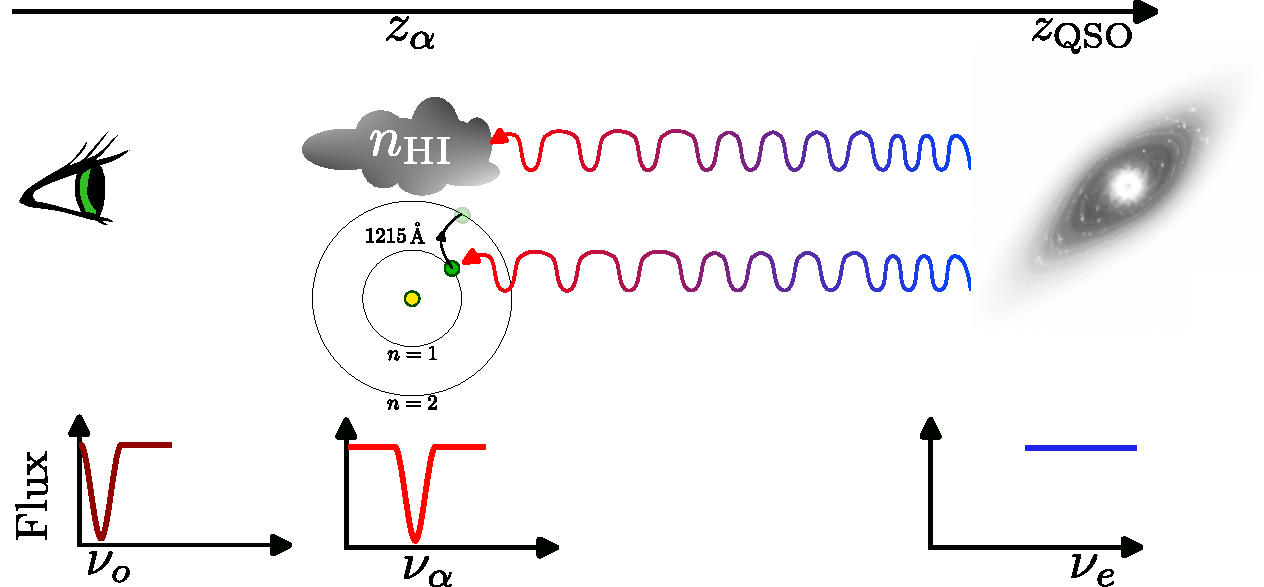
\includegraphics[width=1\linewidth]{img/lyman-alpha.pdf}
    \caption{Illustration of the Lyman-$\alpha$ absorption by neutral hydrogen at $z=z_\alpha$ in the line of sight of a QSO at $z=z_{\text{QSO}}$. In the observer's rest frame, the observed frequency is $\nu_o$. The associated frequency emitted by the QSO is $\nu_e$. }
    \label{fig_ch1:Lyman_alpha_diagram}
\end{figure}
We are interested in studying the effect of the Lyman-$\alpha$ absorbed at $z_\alpha$. The observed flux attenuation at the observed frequency $\nu_0$ is then expressed as $\exp(-\tau_\alpha)$, with $\tau_\alpha$ the Lyman-$\alpha$ opacity at the observed frequency, which depends on the observer's density and the Lyman-$\alpha$ cross-section $\sigma_\alpha(\nu)$. Observe now that since the Lyman-$\alpha$ cross-section is strongly peaked at the resonance $\nu_\alpha$, but can have a non-zero width, a nearby neutral hydrogen cloud might absorb photons at a redshift different to $z_\alpha$ that would have contributed to the observed flux at frequency $\nu_o$. With this consideration, we integrate over the line of sight to obtain the Lyman-$\alpha$ opacity at the observed frequency

\begin{equation}\label{eq_ch1:GP_integral}
    \tau_\alpha(\nu_o)=\int_o^{z_\text{QSO}} n_\text{HI}(z) \sigma_\alpha[\nu_o(1+z)] \differential z.
\end{equation}
If we now take $\sigma_\alpha(\nu)$ to be a Dirac delta centered at the resonance $\nu_\alpha$, and we integrate Equation \ref{eq_ch1:GP_integral} by using \ref{eq_ch1:dl_over_dz} we obtain

\begin{equation}\label{eq_ch1:GP_approx}
    \tau_\alpha(\nu_o)\approx \frac{cn_\text{HI}(z_\alpha)\sigma_\alpha}{H_0\Omega_\text{m}^{1/2} (1+z)^{1/3}},
\end{equation}
where now $\sigma_\alpha=4.5 \times 10^{-18}$cm$^2$ is to total Lyman-$\alpha$ cross-section.
Equation \ref{eq_ch1:GP_approx} is known as the Gunn-Peterson approximation for the Lyman-$\alpha$ opacity of the IGM \cite{GunnPeterson}. Equation \ref{eq_ch1:GP_approx} demonstrates that quasar spectra are a useful probe of the intergalactic neutral hydrogen density.





A more precise analysis of Equation \ref{eq_ch1:GP_integral} can be done if we do not approximate $\sigma_\alpha$ as a Dirac delta. Instead, we can include the two main broadening effects in the absorption cross-section: the natural broadening and the thermal broadening. The natural broadening is a result of quantum processes and generates a Lorentzian profile, while the thermal one is due to the microscopic Doppler effect of thermal motion and generates a Gaussian profile. The resulting combination of both the Lorentzian and Gaussian profiles is known as a Voigt profile. It is a non-analytical function with a Gaussian-like shape but heavier tails:
\begin{equation}\label{eq: Voigt}
    V(x,y)=\frac{Y}{\pi}\int_{-\infty}^{\infty}\frac{e^{-t^2}}{(x-t)^2+y^2} dt.
\end{equation}
The Lyman-$\alpha$ absorption cross-section described by the Voigt profile is then
\begin{equation}
    \sigma_\alpha(\nu)=\frac{cI_\alpha}{b\sqrt{\pi}} V\left(\frac{x(\nu-\nu_\alpha)}{b\nu_\alpha}, \alpha  \right),
\end{equation}
where $b=\frac{\sqrt{2k_BT}}{m_p}$ is the Doppler parameter at temperature $T$, $\nu_\alpha \approx 2.47\times 10^{15}$ Hz is the $Lyman-\alpha$ frequency, $I_\alpha \approx 4.45\times 10^{-18}$ cm$^{-2}$ is the total absorption cross-section \cite{Mo2010} and $\alpha$ is the recombination coefficient, which also depends on the temperature.
The Lyman-$\alpha$ cross-section is then peaked at the resonant frequency, and broadened by the temperature and the recombination rate. Now, consider a sightline of gas absorbing Lyman-$\alpha$ photons. Peculiar bulk velocities $v$ of the gas will add an additional Doppler effect in the cross-section as
\begin{equation}\label{eq:cross section}
    \sigma_\alpha(\nu)=\frac{cI_\alpha}{b\sqrt{\pi}} V\left(\frac{x(\nu-\nu_\alpha)}{b\nu_\alpha} +\frac{v}{b}, \alpha  \right).
\end{equation}
We can now integrate Equation \ref{eq:cross section} along the sightline to obtain the Lyman-$\alpha$ opacity $\tau$ as
\begin{equation}
    \tau = \int n(t)\sigma_\alpha(\nu_\alpha a(t_0)/a(t)) dt,
\end{equation}
where $n$ is the neutral hydrogen density and $t_0$ the emisison time.
Recalling that the comoving distance $x$ is related to redshift and time as 
\begin{equation}
    dx=\frac{c}{H(z)}dz=c(1+z)dt,
\end{equation}
we get that the Lyman-$\alpha$ optical depth $\tau$ can be obtained from the neutral hydrogen gas properties along the sightline as follows:
\begin{equation}\label{eq:lyman opacity}
    \begin{aligned}\tau(z_0)&=\frac{cI_\alpha}{\sqrt{\pi}}\int dx\frac{n_{\mathrm{H}}[x,z(x)]}{b[x,z(x)][1+z(x)]}\times V\left\{\frac{c[z(x)-z_0]}{b[x,z(x)](1+z_0)}+\frac{v[x,z(x)]}{b[x,z(x)]},\alpha\right\}\end{aligned}
\end{equation} 
where $n_\text{H}$ is the neutral hydrogen density, $b=\sqrt{\frac{2k_BT}{m_p}}$, $v$ is the peculiar velocity along the sightline, $m_p$ is the proton mass, $k_B$ is Boltzmann's constant, $\alpha$ is the recombination coefficient, $c$ is the speed of light, $I_\alpha$ is the total cross-section for Lyman-$\alpha$ absorption and $V$ is the Voigt function \cite{Choudhury_2001}. Since the Lyman-$\alpha$ flux $F=e^{-\tau}$ field depends on the properties of the absorbing gas, it contains information about the state of the IGM. The set of Lyman-$\alpha$ absorption features on the spectrum of a quasar is known as the Lyman-$\alpha$ forest. In Figure \ref{fig:forest} we show the spectrum of the quasar 1422+23, taken with the Keck HIRES instrument, and featuring a Lyman-$\alpha$ forest.

\begin{figure}[ht]
    \centering
    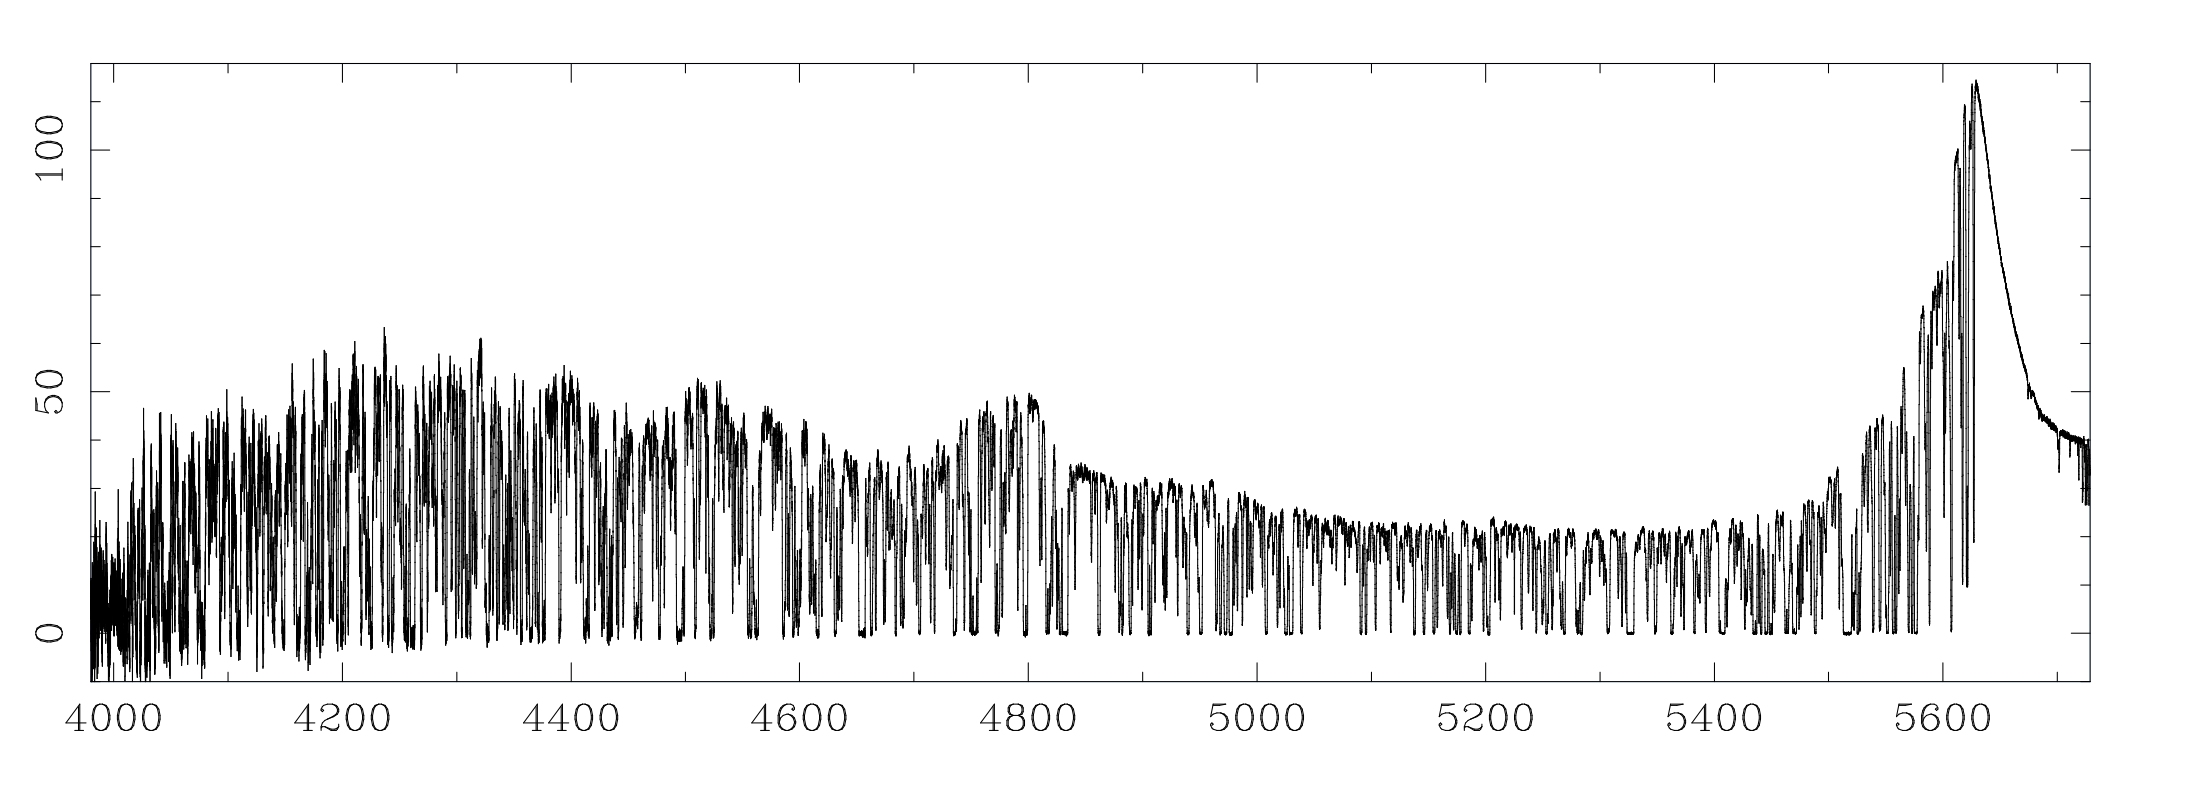
\includegraphics[width=1\linewidth]{img/ML/forest.png}
    \caption{High resolution (FWHM $\sim$ 6.6 km/s) spectrum of the $z = 3.62$ quasar 1422+23, taken with the Keck HIRES (signal-to-noise ratio $\sim$ 150 per resolution element, exposure time 25000 s). The horizontal axis is in units of observed wavelength in angstroms. Extracted from \cite{Rauch_1998}}
    \label{fig:forest}
\end{figure}

\section{Dark matter}\label{sec:DM}

Many aspects of the large-scale structure of the Universe can be understood by including a \emph{cold dark matter} (CDM) component that represents $\sim 26 \%$ of the critical density \cite{planck2014}. In the standard cosmological model, $\Lambda$CDM, dark matter is an important ingredient for structure formation in the Early Universe. However, its precise nature remains an outstanding problem both in cosmology and particle physics. With more exotic DM candidates, such as primordial black holes, heavily constrained, it is likely that DM consists of some undiscovered elementary particle(s) produced early in the history of the universe \cite{Villanueva_Domingo_2021}. There are multiple pieces of evidence supporting the CDM model, including the rotation curves of spiral galaxies and the kinematics of colliding clusters such as the Bullet cluster \cite{Navarro1996}, \cite{de_Blok_2008}.

According to the current paradigm \cite{Mo2010}, dark matter halos are the structures that host galaxies. They form through the gravitational collapse of non-linear perturbations in the primordial density field that serve as the first seeds for the formation of structures. Dark matter halos then grow by accreting material from their surrounding (such as the IGM). The properties of dark matter have then a direct influence on the properties of galaxies (formation, clustering, merging, etc.) and in the general distribution of matter in the Universe.

The evolution of the primordial fluctuations is not only determined by the gravitational clumping of matter but also by
the effect of random particle motions, which leads to a damping of the density peaks and perturbations. The scale at which this happens is set by the free-streaming length defined as the comoving distance travelled by a particle before a time $t$:
\begin{equation}
    \lambda_\mathrm{FS}=\int_0^t\frac{v(t')}{a(t')}dt'.
\end{equation}
$\Lambda$CDM models dark matter as pressureless and only interacting through gravity. Moreover, CDM decouples from the primordial plasma when it is already non-relativistic.
As a consequence, CDM has no significant amount of free-streaming, and (thermal)pressure does not hinder its clustering, which enables the formation of large hallos that can be as massive as $10^15$ M$_\odot$.

On large scales, the predictions of $\Lambda$CDM have been amply tested and are in good agreement with observations \cite{Dalal2002}, \cite{VanWaerbeke2004}, \cite{Eisenstein2005}. In contrast, on scales smaller than $\sim 10$ kpc, potential tensions between CDM predictions and observations might exist, including the ``core-cusp" problem related to the DM density profile in halos, or the ``too big to fail" problem linked to the number density of high-luminosity satellites in sub-halos \cite{Moore1994}, \cite{Boylan_Kolchin_2011}, \cite{Weinberg_2015}. Even if the inclusion of complex baryonic feedback processes can alleviate the aforementioned potential discrepancies, alternative models to CDM are worth exploring \cite{Vogelsberger2014}.  

As a consequence of these possible tensions, there have been a multitude of DM candidates to CDM. Such variations have included self-interactions \cite{Spergel2000} and fuzzy DM which leads to wave-like features in the density fields \cite{Hu2000}. Most alternative models retain the success of CDM on large scales while reproducing the desired features on smaller scales. Simulating how variations of CDM affect the evolution of structures in the Universe is highly non-trivial. Perhaps the simplest models that are viable to explore are warm(hot) dark matter WDM (HDM). Such candidates are usually classified according to their free-streaming scales. While for CDM particles $\Lambda_\mathrm{FS}$ is negligible at the scales of cosmological structure formation, for HDM models, such as light neutrinos, $\Lambda_\mathrm{FS}$ smooths out gravitational clustering even at galaxy cluster scales, leading to tight constraints on such models \cite{Hannestad_2004}. In between HDM and CDM, WDM offers an intermediate range of free-streaming scales that could potentially be compatible with the observed evolution of the Universe. In this work we focus on thermal relic WDM models, which include potential particles such as gravitinos or sterile neutrinos that were coupled to the original plasma in the Early Universe \cite{Viel_2005}. For such models, WDM is a particle of mass in the scale of the KeV. A WDM particle with a mass of $1$ KeV would have a free-streaming scale of $\Lambda_\mathrm{FS} \sim 0.3 Mpc$. In general, more massive particles are associated with smaller velocities and hence smaller $\Lambda_\mathrm{FS}$. The nature of WDM suppresses the total matter power spectrum on scales smaller than their free-streaming. That is, the less massive a WDM model is, the more the power spectrum is suppressed at small scales, and the more the density features of the density field are smoothed out.
To illustrate this process, consider Figure \ref{fig:villasenor_wdm}, which shows a simulated density field of the IGM as a function of redshift, and the WDM model mass. On the horizontal axis, the time evolution shows how gravity collapses dense regions into structures. On the vertical axis, the WDM free-streaming length suppresses small-scale clustering. 

\begin{figure}[ht]
    \centering
    \includegraphics[width=\textwidth]{img/ML/villa_wdm.png}
    \caption{Baryonic density plot of the IGM as a function of redshift, and the WDM model mass. On the horizontal axis, the time evolution shows how gravity collapses dense regions into structures. On the vertical axis, the WDM free-streaming length suppresses small-scale clustering. Extracted from \cite{Villasenor_2023}.}
    \label{fig:villasenor_wdm}
\end{figure}

Constraining WDM in the cosmological context involves understanding and determining which WDM model masses are compatible with the Universe we observe. Since the effect of WDM on structure formation is too complex, this process typically involves comparing simulations with observations: cosmological simulations are run for multiple WDM models, and the resulting properties are statistically compared to observations to rule out a certain range of masses. In Section \ref{chap:sherwood} we discuss how such simulations work and how WDM models are included in them.

Observations that have been used to constrain DM models include gravitational lensing \cite{Massey_2010} or the study of dwarf galaxies \cite{Calore_2018}. In this work, we focus on the Lyman-$\alpha$ forest that was introduced in Section \ref{sec:IGM}. As we have discussed, the properties of the Lyman-$\alpha$ forest depend on the properties of the IGM, and in particular on its matter distribution, which is directly linked with the WDM particle mass. Many efforts have been made to constrain WDM by comparing the Lyman-$\alpha$ forest generated by WDM models to the observed one in quasar spectra\cite{sherwood_wdm}, \cite{Villasenor_2023}, \cite{Viel_2005}.

\section{Structure of this work}
Building on previous efforts in the literature (most notably \cite{nasir2024deep}), in this work we explore the possibility of reconstructing the neutral hydrogen density field directly from the Lyman-$\alpha$ forest and whether such information can be used to constrain WDM. This reconstruction step involves careful analysis and represents a challenge at the frontier of the current efforts by the community. While the current state-of-the-art techniques extract information from the Lyman-$\alpha$ forest by using summary statistics, recovering the
non-observable physical fields of relevance would allow for the extraction of all the richness of information present in the forest. In particular, such techniques would allow for the mapping of the neutral hydrogen distribution in the Universe at the scales and redshifts where the forest is observable.

We begin in Section \ref{chap:sherwood} by exploring how WDM models affect the Lyman-$\alpha$ forest and the underlying neutral hydrogen field. For that purpose, we introduce a set of cosmological simulations that will be at the core of this work, the \texttt{SHERWOOD} simulation suite. We discuss the main aspects of such simulated data, including the cosmological code used in them. We conclude Section \ref{chap:sherwood} with a statistical analysis of the Lyman-$\alpha$ forest. Section \ref{chap: deep learning} is devoted to introducing the deep learning machinery used to reconstruct the neutral hydrogen density field from the Lyman-$\alpha$ forest flux. We begin by motivating the use of machine learning techniques and describing the basic concepts related and implementations related to such tools. Next, we discuss the motivation, architecture and implementation of the Bayesian neural network used in this regression task. We describe how we train the model using simulated data, evaluate its performance and robustness, and discuss some relevant questions about its internal dynamics. Armed with a machine learning pipeline that can reconstruct the neutral hydrogen density field from observed Lyman-$\alpha$ skewers, we are set to use this information in Section \ref{sec: inference pipeline} to constrain WDM. We discuss and implement a statistical pipeline to convert the recovered neutral hydrogen density field into WDM constraints. We extensively test this pipeline first on simulated data, from which we know the DM model used. Then, we turn our attention to real observational data and apply our technique to a set of quasar sightlines obtained from state-of-the-art spectrographs. We compare our results with the most up-to-date constraints in the literature, both in terms of tightness and efficiency in data usage.


\chapter{Simulating the Lyman-alpha forest} \label{chap:sherwood}
In Section \ref{chapter:intro} we discussed how the Lyman-$\alpha$ forest is sentive to multiple physical parameters, such as the low-gas temperatures, velocities, densities, etc. Each possible state of the IGM's ionized low-density gas can lead to different absorption spectra and different forms of the forest. Hydrogen reionisation finishes at $z<5.3$ \cite{Bosman_2022}. Hence, at low redshift, there is no neutral hydrogren to produce absoprtion features, and we have complete transmission of the Lyman-$\alpha$ flux withput features, which means we cannot extract information about the IGM through this process. On the other end, at high redshifts, $z>6$, the hydrogren is not sufficiently ionized and total absoprtion of quasar continuum by neutral hydrogen generates long Gunn-Peterson troughs.
Hence, the Lyman-$\alpha$ forest at $2<z<5$ is a powerful probe of the state of the IGM at scales and redshifts not accessible by any other observable \cite{Hernquist__1996}. As a consequence, simulations of the Lyman-$\alpha$ forest are typically carried out at said redshift range.














\section{The Sherwood simulation suite}\label{sec:sherwood suite}
Lyman-$\alpha$ simulations are typically based on cosmological simulation codes.
In this work, we will mainly focus on the \texttt{SHERWOOD} simulation suite\footnote{\url{https://www.nottingham.ac.uk/astronomy/sherwood/}} \cite{Bolton_2016}, which are based on the \texttt{GADGET-2} developped by Volker Springel \cite{Springel_2005}. \texttt{GADGET-2} uses the Lagrangian formulation of fluid dynamics to trace the evolution of fluid particles.


\texttt{GADGET-2} traces non-interacting dark matter (as described by the collisionless Boltzmann equation) by sampling phase space with a finite number of particles and solving their dynamics. The dynamics of such particles are subject to the Hamiltonian

\begin{equation}
        H=\sum_i\frac{\boldsymbol{p}_i^2}{2 m_i a(t)^2}+\frac12\sum_{ij}\frac{m_im_j \varphi(\boldsymbol{x}_i-\boldsymbol{x}_j)}{a(t)},
\end{equation}
where $\boldsymbol{x}$ are the comoving positions, $a$ the scale factor, $\boldsymbol{p}$ the canonical momenta and $m$ the particle masses.

On the other hand the gas particles are traced using Smoothed Particle hydrodynamics (SPH). SPH describes a fluid by means of a finite set of tracer particles that sample the local state of the fluid. Then, smooth quantities are obtained by using a smoothing kernel to interpolate between the tracer's properties. The equation of motion for the SPH particles is then
\begin{equation}
        \frac{\mathrm{d}\boldsymbol{v}_i}{\mathrm{d}t}=-\sum_{j=1}^Nm_j\left[f_i\frac{P_i}{\rho_i^2}\nabla_iW_{ij}(h_i)+f_j\frac{P_j}{\rho_j^2}\nabla_iW_{ij}(h_j)\right],
\end{equation}
with
\begin{equation}
        f_i=\left[1+\frac{h_i}{3\rho_i}\frac{\partial\rho_i}{\partial h_i}\right]^{-1}.
\end{equation}
Here, $W$ is the smoothing kernel, $h_i$ are smoothing lengths parameters, $P_i$ are the pressures associated with the particles and $\rho_i$ their densities. For more details see the original paper \cite{Springel_2005}.



Gravity is the driving force for strucuture formation in the Universe, but its long-range nature makes it challenging to implement efficiently. \texttt{GADGET-2} implements a gravitational algorithm that ensure sufficient spatical adaptability by using a hierarchical multipole expansion. By using a tree-like approach, we can compute the force applied to a particle in compelcity $\mathcal{O}(log(N))$ instead of $\mathcal{O}(N)$, where $N$ is the number of particles. The algorithm works by subdividing the space into octants, such that each leaf contains a single particle. The net force on a particle is then calculated by traversing the octree and replacing distant cell by a single body, thus reducing the number of needed terms. This process is also called the \emph{Barnes-Hut} algorithm, see Figure \ref{fig: 2D Barnes Hut} for an Illustration of it.

\begin{figure}
        \centering
        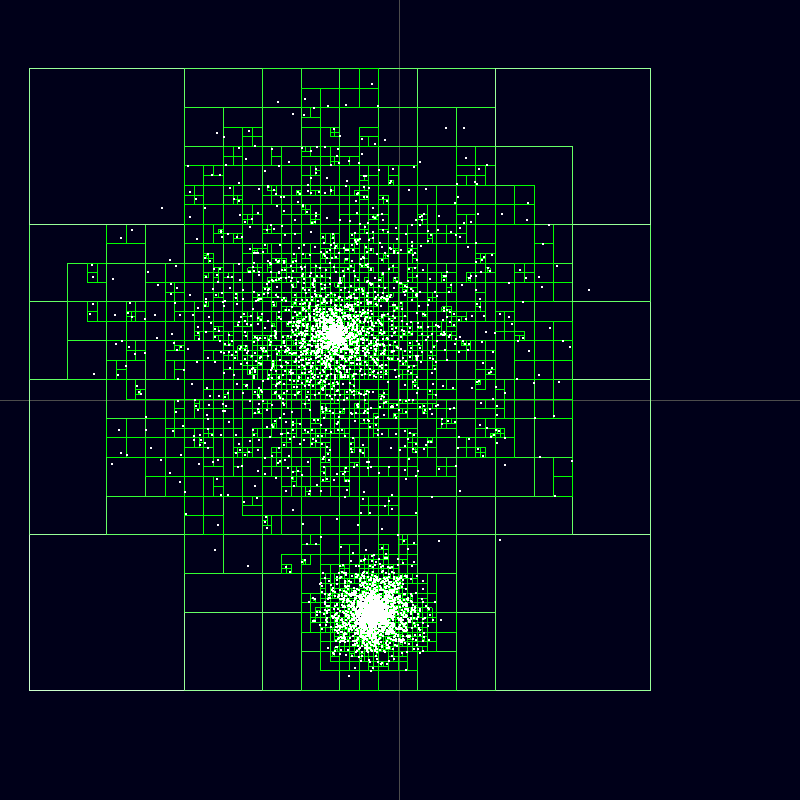
\includegraphics[width=0.5\textwidth]{img/ML/Barnes_hut_tree.png}
        \caption{An octree generated using the Barnes-Hut algorithm for a set of particles (in white) in a 2D space.}
        \label{fig: 2D Barnes Hut}     
\end{figure}

The  dynamics of the system are then governed by the interaction potential
\begin{equation}
        \nabla^2\varPhi(x)=4\pi G(\rho-\overline{\rho}).
\end{equation}

The \texttt{SHERWOOD} suite implements the effect of WDM by suppressing the initial power spectrum as described in \cite{Viel_2005}. In this approach, the effects of the warm dark matter free-streaming length on the matter distribution are described by a transfer function $T(k)$

\begin{equation}
        T(k)^2=\frac{P(k)_{\Lambda\mathrm{WDM}}}{P(k)_{\Lambda\mathrm{CDM}}},
\end{equation}
where $P(k)$ is the matter power spectrum (see Section \ref{sec:statistics sher} for more details). For pure thermal WDM models, as the ones we consider in this work, the transfer function can be approximated by:

\begin{equation}
        T(k)=[1+(\alpha k)^{2\nu}]^{-5/\nu},
\end{equation}
where $\nu\approx 1.12$ and $\alpha$ is related to the WDM particle mass by
\begin{equation}
        \alpha \propto \left( \frac{m_\mathrm{WDM}}{1 \mathrm{KeV}} \right)^{-1.11}.
\end{equation}
The initial coniditons are then generated at $z=99$ using the matter power spectrum, see \cite{Bolton_2016} for more details.

On top of the hydrodynamics and gravity, the Sherwood code implements a variety of relevant physical process that contribute to the state of the IGM and the Lyman-$\alpha$ forest. The simulations calculate the photo-ionisation and photo-heating for the gas (assumed to be in ionisation equilibrium) by using a uniform ionising UV backgorund as described in \cite{Haardt2012}. Instead of following the star formation process, dense and cold gas particles ($\Delta>1000$ and $T<10^5$K) are converted into collisionless particles. The runs discussed here do not include AGN feedback, which has a small effect on the Lyman-$\alpha$ forest at high redshift.

In our work, we use a subset of the \texttt{SHERWOOD} suite described in \cite{sherwood_wdm}. All boxes are of size 20h$^{-1}$cMpc, with $2\times 1024^3$ particles. The mass for gas and dark matter particles is, respectively, $5.37\times 10^5h^{-1}M_\odot$ and $9.97\times 10^4h^{-1}M_\odot$. In Table \ref{tab: Sherwood} we summarise the runs used in this work.


\begin{table}
        \caption[]{List of the \texttt{SHERWOOD} runs used in the work.
        All box sizes are 20h$^{-1}$. The table shows the mean temperature of the IGM $T_0$ at redshift $z=4.4$, the redshift of reionisation, and the set of WDM masses included. We work with the inverse WDM mass and consider 0 to correspond to the CDM reference run.}
           \label{tab: Sherwood}
       $$ 
           \begin{array}{p{0.3\linewidth}ccc}
              \hline
              \noalign{\smallskip}
              Run      &  T_0 {[\mathrm{K}]}\ (z=4.4) &z_\mathrm{rei}^\mathrm{end}& \mathrm{WDM} [\mathrm{KeV}^{-1}] \\ 
              \noalign{\smallskip}
              \hline
              \noalign{\smallskip}
              L20-ref & 10556 &6.00&\{0,\frac{1}{2}, \frac{1}{3}, \frac{1}{4}, \frac{1}{8}, \frac{1}{12} \}     \\
              L20-ref-hot           & 12161&6.01  &\texttt{"}\\
              L20-ref-cold     & 9862  &5.98&       \texttt{"}     \\
              \noalign{\smallskip}
              \hline
           \end{array}
       $$ 
     \end{table}
The reference run is L20-ref. We will refer to the dataset consisting on this run as \texttt{SHERWOOD} in what follows. We also use two runs with varied thermal parameters L20-ref-hot and L20-ref-cold. The dataset consisting on all 3 runs will be denoted as \texttt{SHERWOOD THERMAL} in this work.

We conclude this section by visually inspecting the \texttt{SHERWOOD} data, to give a broad intuition of how the IGM fields behave. In Figure \ref{fig: 2D density image} we show a 2D neutral hydrogren overdensity field generated using the \texttt{SHERWOOD} suite at $z=4.2$ for multiple WDM models. The simulation size is 20h$^{-1}$cMpc. On the horizontal axis, we linearly interpolate the density field for the WDM models to show the effect or multiple DM candidates on the density field.
\begin{figure}[ht]
        \centering
        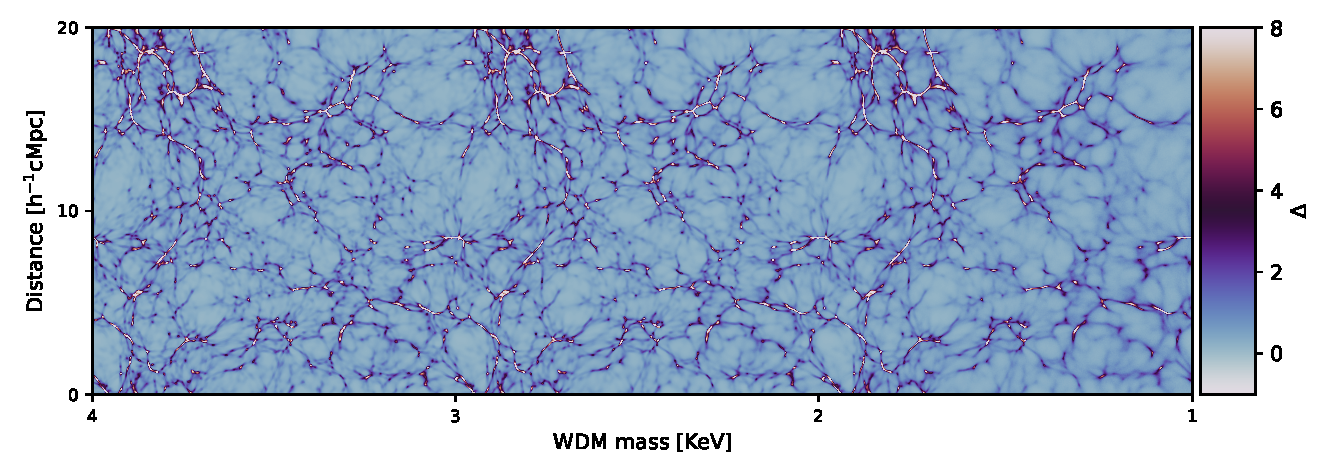
\includegraphics[width=0.99\textwidth]{img/ML/density_image_wdm.pdf}
        \caption{A 2D neutral hydrogren overdensity field generated using the \texttt{SHERWOOD} suite at $z=4.2$ for multiple WDM models. The simulation size is 20h$^{-1}$cMpc. On the horizontal axis, we linearly interpolate the density field for the WDM models to show the effect or multiple DM candidates on the density field.}
        \label{fig: 2D density image}     
\end{figure}
In Figure \ref{fig: 1D density skewer} we show a  1D neutral hydrogren overdensity field at $z=4.4$ along a 20h$^{-1}$cMpc Sherwood skewer for the CDM model run. Note how the density field is periodic, since the Sherwood simulations implement periodic boundary conditions. Most of the gas is close to the mean density $\Delta \sim 1$, with local overdensities that can generate $\Delta \sim 20$ corresponding to regions where there is a positive flow of gas.
\begin{figure}
        \centering
        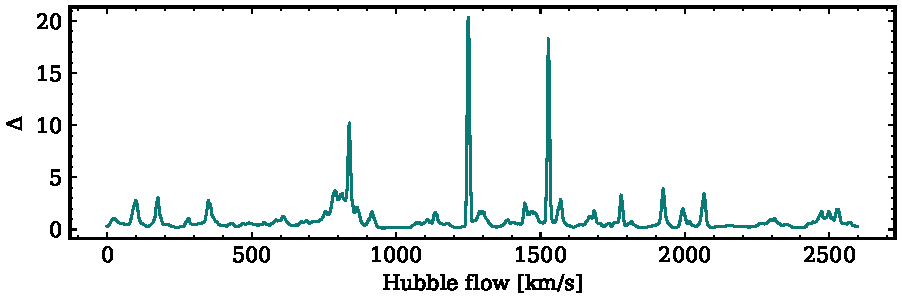
\includegraphics[width=0.99\textwidth]{img/ML/Skewer_density.pdf}
        \caption{A 1D neutral hydrogren overdensity field at $z=4.4$ along a 20h$^{-1}$cMpc Sherwood skewer for the CDM model run.}
        \label{fig: 1D density skewer}     
\end{figure}










\section{Obtaining mock Lyman-alpha skewers from cosmological simulations}
The \texttt{SHERWOOD} simulation suite described in Section \ref{sec:sherwood suite} generates as output the low-density IGM's overdensity, hydrogen neutral fraction, sightline velocity, temperature and the redshift of every pixel. For each run, recall that those fields form a $(5000,2048)$ array for all 5000 sightlines. From such data, we can use Equation \ref{eq:lyman opacity} to compute the simulated Lyman-$\alpha$ sightlines. We implement the code in Python and descritise the integral in Equation \ref{eq:lyman opacity} to sum over all 2048 pixel in the skewer. We use the values for the recombination coefficient in \cite{Luki__2014}.

In our code, we consider two different implementations for the Voigt profile, which is non-analitical. Firstly, we exploit the relationship with the Faddeeva function. The Faddeeva function is implemented in Scipy under \texttt{scipy.special.wofz} for optimized computation. Let us prove a relationship between the Faddeeva function and the Voigt function. Let $z=x+iy$.
The Faddeeva function $w(z)$ is defined as

\begin{equation}
    w(z)=\frac{i}{\pi} \int_{-\infty}^{\infty} \frac{e^{-t^2}}{z-t}dt
\end{equation}
and we have 
\begin{equation}\label{eq:FAD}
    Re \left( w(z=x+iy) \right)=V(x,y)
\end{equation}
The proof is trivial:
\begin{equation}
    \begin{split}
        Re\ i \int_{-\infty}^{\infty} \frac{e^{-t^2}}{z-t}dt
        &= Re\ i \int_{-\infty}^{\infty} \frac{e^{-t^2} (x-t-iy)}{(x-t)^2+y^2}dt\\
        &=y\int_{-\infty}^{\infty} \frac{e^{-t^2}}{(x-t)^2+y^2}dt
    \end{split}
\end{equation}

We consider a second implementation of the Voigt function by leveraging a power series expansion known as the Tepper-Garcia approximation \cite{Tepper_Garc_a_2006}. The Tepper-Garcia approximation is
\begin{equation}\label{eq:Tepper}
        V(x,y)\approx e^{-x^2}\left( 1-\frac{2y}{\sqrt{\pi}} K(x) \right),
\end{equation}
with
\begin{equation}
        K(x)=\frac1{2x^2}\left[(4x^2+3)\left(x^2+1\right)\mathrm{e}^{-x^2}-\frac1{x^2}(2x^2+3)\sinh x^2\right].
\end{equation}
As can be seen from the Tepper-Garcia approximation, the Voigt function is a modified Gaussian function. Figure \ref{fig: VOIGT APPROX} shows a comparison between the Faddeeva and Tepper-Garcia implementations of the Voigt function for multiple values of the $y$ parameter. Since in our problem typical recombination coefficients are of order $10^{-10}$cm$^3$s$^{-1}$, both implementations are essentially equivalent.

\begin{figure}[ht]
        \centering
        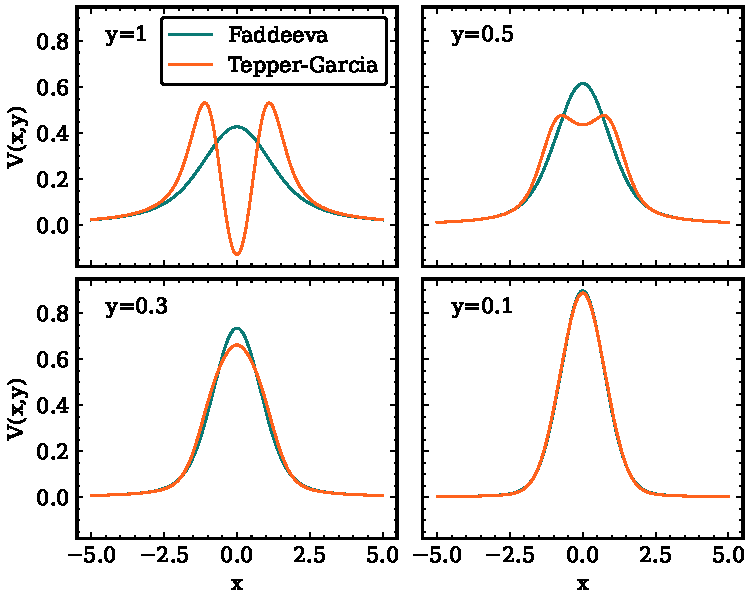
\includegraphics[width=0.8\textwidth]{img/ML/TP-FA.pdf}
        \caption{Comparison of the Voigt function $V(x,y)$ that is included in Equation \ref{eq:lyman opacity} implemented using the relation with the Faddeeva function in Equation \ref{eq:FAD} and the Tepper-Garcia approximation in Equation \ref{eq:Tepper}.}
        \label{fig: VOIGT APPROX}     
\end{figure}

An important aspect when simulating Lyman-$\alpha$ sightlines is boundary conditions. In fact, the simulation boxes in the \texttt{SHERWOOD} suite and other cosmological codes implement periodic boundary conditions. This means that a physical quantity $Q$ satisfies
\begin{eqnarray}
        Q(0)=Q(L),
\end{eqnarray}
where $L$ is the length of the simulation box. This condition also applies to the density field, temperature field, etc. Periodic boundary conditions allow implementing relevant physical conditions, such as conserved quantities, in the simulation volume. As a consequence, we would like the optical depth fields generated using the \texttt{SHERWOOD} data to also implement periodic boundary conditions. This will be the case if every pixel in the sightline has the approxmiate same environment has a translational by the skewer length. To achieve this in a computationally efficient manner, observe that in Equation \ref{eq:lyman opacity}, for $\alpha\to 0$, the amplitude of the Voight profile is set by $b(T)\sim 10$ km/s for $T\sim 10^4$. Since the pixel scale is $\sim 1$ km/s, the Voigt profiles only influence neaby pixels. As such, let us fix a pixel $i$ on which we wish to calculate the optical depth. Then, we iterate over all pixels $j$ and evaluate the condition $|z[i]-z[j]| < L/2$. If this condition is true, we use Equation \ref{eq:lyman opacity} to compute the contribution. If the condition is false, then we use the pixel at $z[j]\pm L/2$ that is closer to $z[i]$. This allows us to in include (approximately) periodic boundary conditions with a complexity $\mathcal{O}(N^2)$ where $N$ is the number of pixels. For reference, see the optical depth field in Figure \ref{fig: skewer sherwood}, where we have applied this procedure.



\section{Peculiar velocities and optical depth-weighted quantities}\label{sec: optical depth weighted}
Equation \ref{eq:lyman opacity} relates properties of the low-density hydrogen in the IGM to the Lyman-$\alpha$ flux field. Each density pixel contributes to the optical depth at any fixed pixel by a quantity proportinal to its density and to the absoprtion profile. However, note that the velocity contributes by shifting the center of the absoprtion profile. As a consequence, the small-scale peculiar velocities of the absorbers due to structure formation wash out the correlation between the overdensity $\Delta$ and $\tau$ fields. A second undesirable effect of the velocity is that it can create potential degeneracies between the gas properties and the flux. In fact, The effect of the velocity field can be captured by considering a shifted density field generating the same flux field. These two problems mean that it is not feasible to recover the real $\Delta$ from the flux. To better correlate the flux features with the density and temperature features and neglect the effects of peculiar velocities, it is common in the literature to work with optical depth-weighted quantities \cite{_oltinsk__2021}. Such quantites allow for a better identification of the gas associated with a certain absoption profile. Optical depth quantities are highly correlated to real quantities and act as a proxy for the latter \cite{Schaye1999}.

We define the optical depth-weighted overdensity field, $\Delta_\tau$, as
\begin{equation}\label{eq: OD weighted}
        \Delta_{\tau,i}=\sum_j \tau_{ij} \Delta_j /\tau_i,
\end{equation}
where $\tau_{ij}$ is the contribution to optical depth at pixel $i$ by pixel $j$. Equation \ref{eq: OD weighted} can also be used to compute the optical depth-weighted temperature. Figure \ref{fig: skewer sherwood} shows a 20h$^{-1}$cMpc \texttt{SHERWOOD} CDM skewer at $z=4.4$ with 2048 pixels. We show the hydrogen overdensity $\Delta$, temperature $T$ and velocity along the sightline $V$, Lyman-$\alpha$ optical depth and flux computed according to \ref{eq:lyman opacity}. We also show the optical depth-weighted overdensity and temperature, computed according to \ref{eq: OD weighted}. Note how optical depth-weighted fields smooth out fluctuations in the small scales, since Equation \ref{eq: OD weighted} is essentially a weighted convolution. The main effect of optical depth-weighted fields is that they are highly correlated to the flux field, with a limited shifting effect due to local velocities. For instance, consider the optical depth peak at $\sim$880 km/s, which is assocaited with a real $\Delta$ peak at $\sim$840 km/s due to peculiar velocty effects. However, the $\Delta_\tau$ peak closely follows to optical depth peak.

\begin{figure}
        \centering
        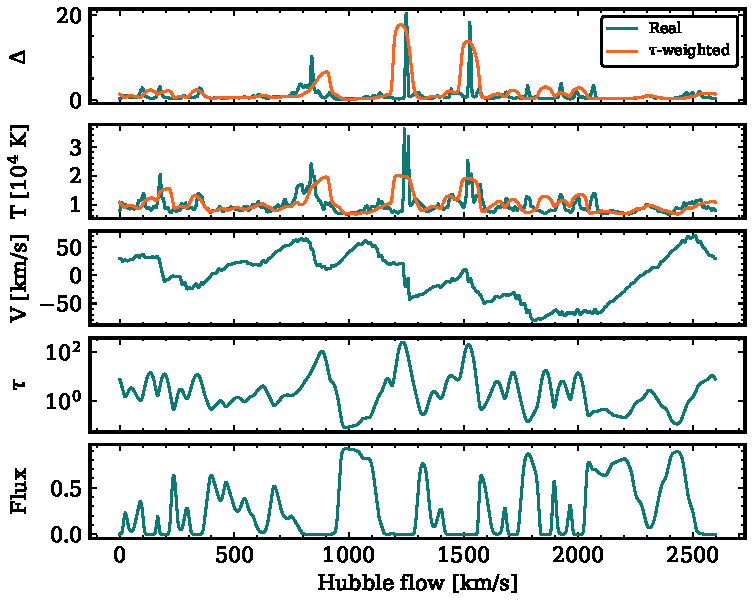
\includegraphics[width=0.95\textwidth]{img/ML/Skewer_OD_quantities.pdf}
        \caption{A 20h$^{-1}$cMpc \texttt{SHERWOOD} CDM skewer at $z=4.4$ with 2048 pixels. We show the hydrogen overdensity $\Delta$, temperature $T$ and velocity along the sightline $V$, Lyman-$\alpha$ optical depth and flux computed according to \ref{eq:lyman opacity}. We also show the optical depth-weighted overdensity and temperature, computed according to \ref{eq: OD weighted}}
        \label{fig: skewer sherwood}     
\end{figure}













\section{Statistical analysis of the effect of dark matter in the flux and density fields}\label{sec:statistics sher}


In Section \ref{sec:sherwood suite} we have presented the \texttt{SHERWOOD THERMAL} simulation suite, which include runs with the same initial seed but different thermal parameters and WDM particle masses. Naturally, challenging such parameters modify the IGM and Lyman-$\alpha$ forest properties. In this section, we explore how the density field and the Lyman-$\alpha$ forest are modified by such parameters within the \texttt{SHERWOOD} suite. In Figure \ref{fig: skewer delta flux} we show an example of this process. The figure shows the $\Delta$ overdensity and flux for 3 different WDM models in ther \texttt{SHERWOOD} suite at $z=4.4$. Note how the CDM skewers shows more fluctuations and pronounced features than the WDM models.

\begin{figure}[ht]
        \centering
            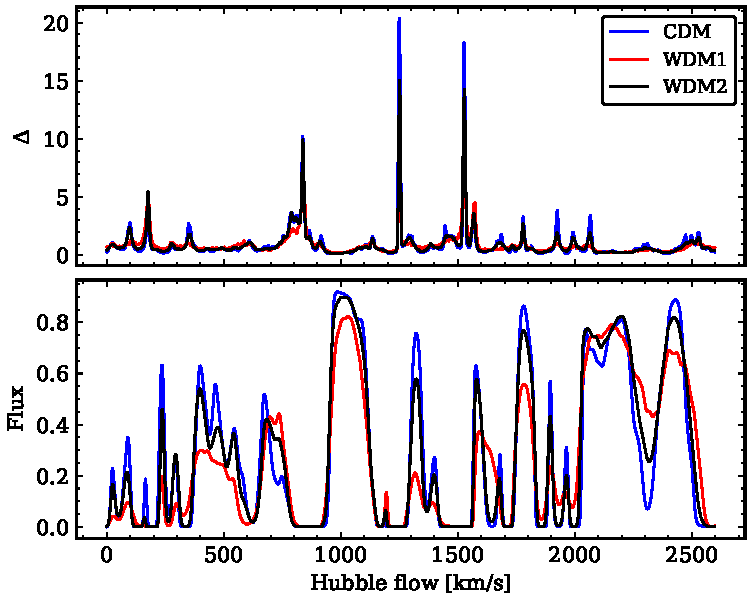
\includegraphics[width=0.99\textwidth]{img/ML/skewer_delta_flux.pdf}
            \caption{The $\Delta$ overdensity and flux for 3 different WDM models in ther \texttt{SHERWOOD} suite at $z=4.4$. Note how the CDM skewers shows more fluctuations and pronounced features than the WDM models.}
            \label{fig: skewer delta flux}
\end{figure}
To quantify this in a more robust and precise way, we leverage two summary statistics, the Probability Distribution Function (PDF) and the Power Spectrum (PS), that aggregate multiple skewers to produce quantities that only depend on the statistical proeprties of the fields, and not on the specific simulation seed for the sightline.

For a given set of sightlines, the PDF of a field is the histogram of values for such field on the array obtained concatenating the skewers. We use Numpy's \texttt{numpy.histogram} to compute it and Rice's rule to obtain the number of bins. According to this rule, for $N$ observed values, the number of bins in the histogram should be $\sim 2N^{1/3}$ \cite{Freedman1981}. For data with 2048 pixels, we use 21 bins. Since in this section we are only interested in quantifying the statistics for every model, we refer to Section \ref{sec:recovered statistics} for a discussion of the uncertainty estimation in field statistics.


\begin{figure}[ht]
        \centering
            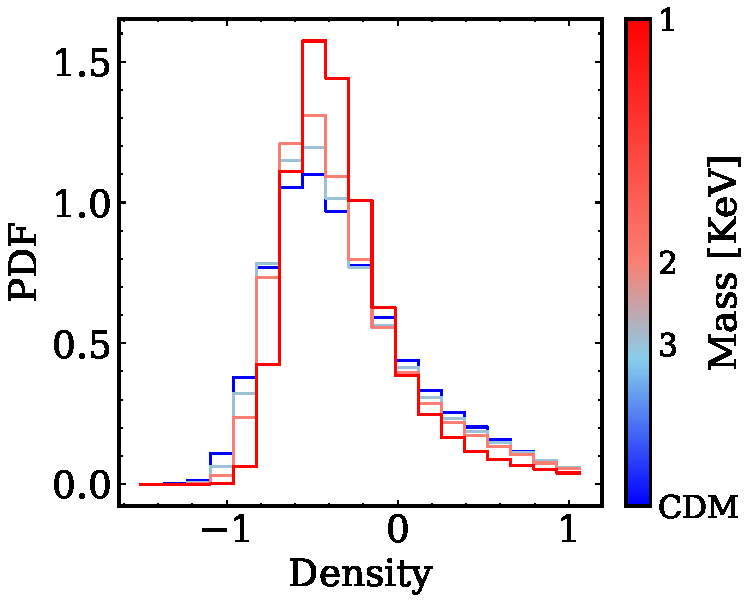
\includegraphics[width=0.8\textwidth]{img/ML/pdf_density_sherwood.pdf}
            \caption{The $\Delta_\tau$ probability distriburion function (PDF) for different WDM models in the \texttt{SHERWOOD} suite.}
            \label{fig: exact density PDF}
\end{figure}


In Figure \ref{fig: exact density PDF} we show the $\Delta_\tau$ PDF at $z=4.4$ for different WDM particle masses in the \texttt{SHERWOOD} suite. Note how low mass models tend to have a more localised distribution near the mean, which reflects the observation from Figure \ref{fig: skewer delta flux} that such models have smoother fields. In contrast, the CDM model has a greater variance, reflecting the fact that more pronounced features occur, which leads to more extreme values for the fields. 

The PDF quantifyies how often a certain value occurs, but not the correlations in the field. To study the oscilattions in the fields it is common in the literature to use the Power Spectrum (PS) \cite{McDonald_2006,Ravoux_2023}. The PS is defined in Fourier space of the relevant field, up to a normalisation factor. Here, we focus on the Lyman-$\alpha$ flux field, $F$, since it has been measured from multiple quasar samples. Since we are only interested in how $F$ oscilates, we consider the flux contrast

\begin{equation}\label{eq: flux contrast}
        \delta F=\frac{F}{\overline{F}} -1,
\end{equation}
where $\overline{F}$ is the mean value of the field. The power spectrum $P_k$ is defined as the modulus of the normalised Fourier transform of $\delta F$:

\begin{equation}\label{eq: PS def}
        P_k = \left| \mathcal{F}(\frac{1}{N} F)  \right| ^2,
\end{equation}
where $N$ is the number of pixels on a sightline (2048 for \texttt{SHERWOOD}) and $\mathcal{F}$ denotes the (Fast) Fourier Transform operator. Note that, by the Wiener-Khinchin theorem, the power spectrum is just the Fourier transform of the autocorrelation function of the $\delta F$. We compute the PS using Numpy's \texttt{numpy.fft} class. The wavenumber $k$ are binned in log space, with a spacing of $\Delta log(k)=0.1$ in the same manner as \cite{Boera_2019}. The compare the PS from the \texttt{SHERWOOD} data to real observations, we normalise the flux field to match the mean observed flux in \cite{Becker_mean_flux}. We do this by introducing a factor $a$ in the optical depth such that $F=e^{-a\tau}$ matches the mean observed flux at every redshift. Figure \ref{fig: sherwood exact PS} shows the Lyman-$\alpha$ flux power spectrum for different WDM models in the \texttt{SHERWOOD} simulation suite, compared to the observed PS by \cite{Boera_2019}. We begin by observing that WDM models have to effect of supressing structure only in the small scales (high $k$ values). At large scales, all WDM models have a similar power spectrum. Lower masses suppress the PS more than WDM models close to CDM.
In Figure \ref{fig: sherwood exact PS}, we observe a systematic bias where the Sherwood CDM power spectrum underestimates the observed power spectrum in \cite{Boera_2019}. In the original Sherwood publication \cite{Bolton_2016}, a continuous bias correction factor is applied to the flux in order to forward model the skewers, in addition to matching the observed effective optical depth. This bias correction, which has not been incorporated in this work, could be the origin of the differences observed in the figure. In the rest of the work, we will use the PDF statistic when constraining WDM, so that this PS bias will not be a concern.

\begin{figure}[ht]
        \centering
        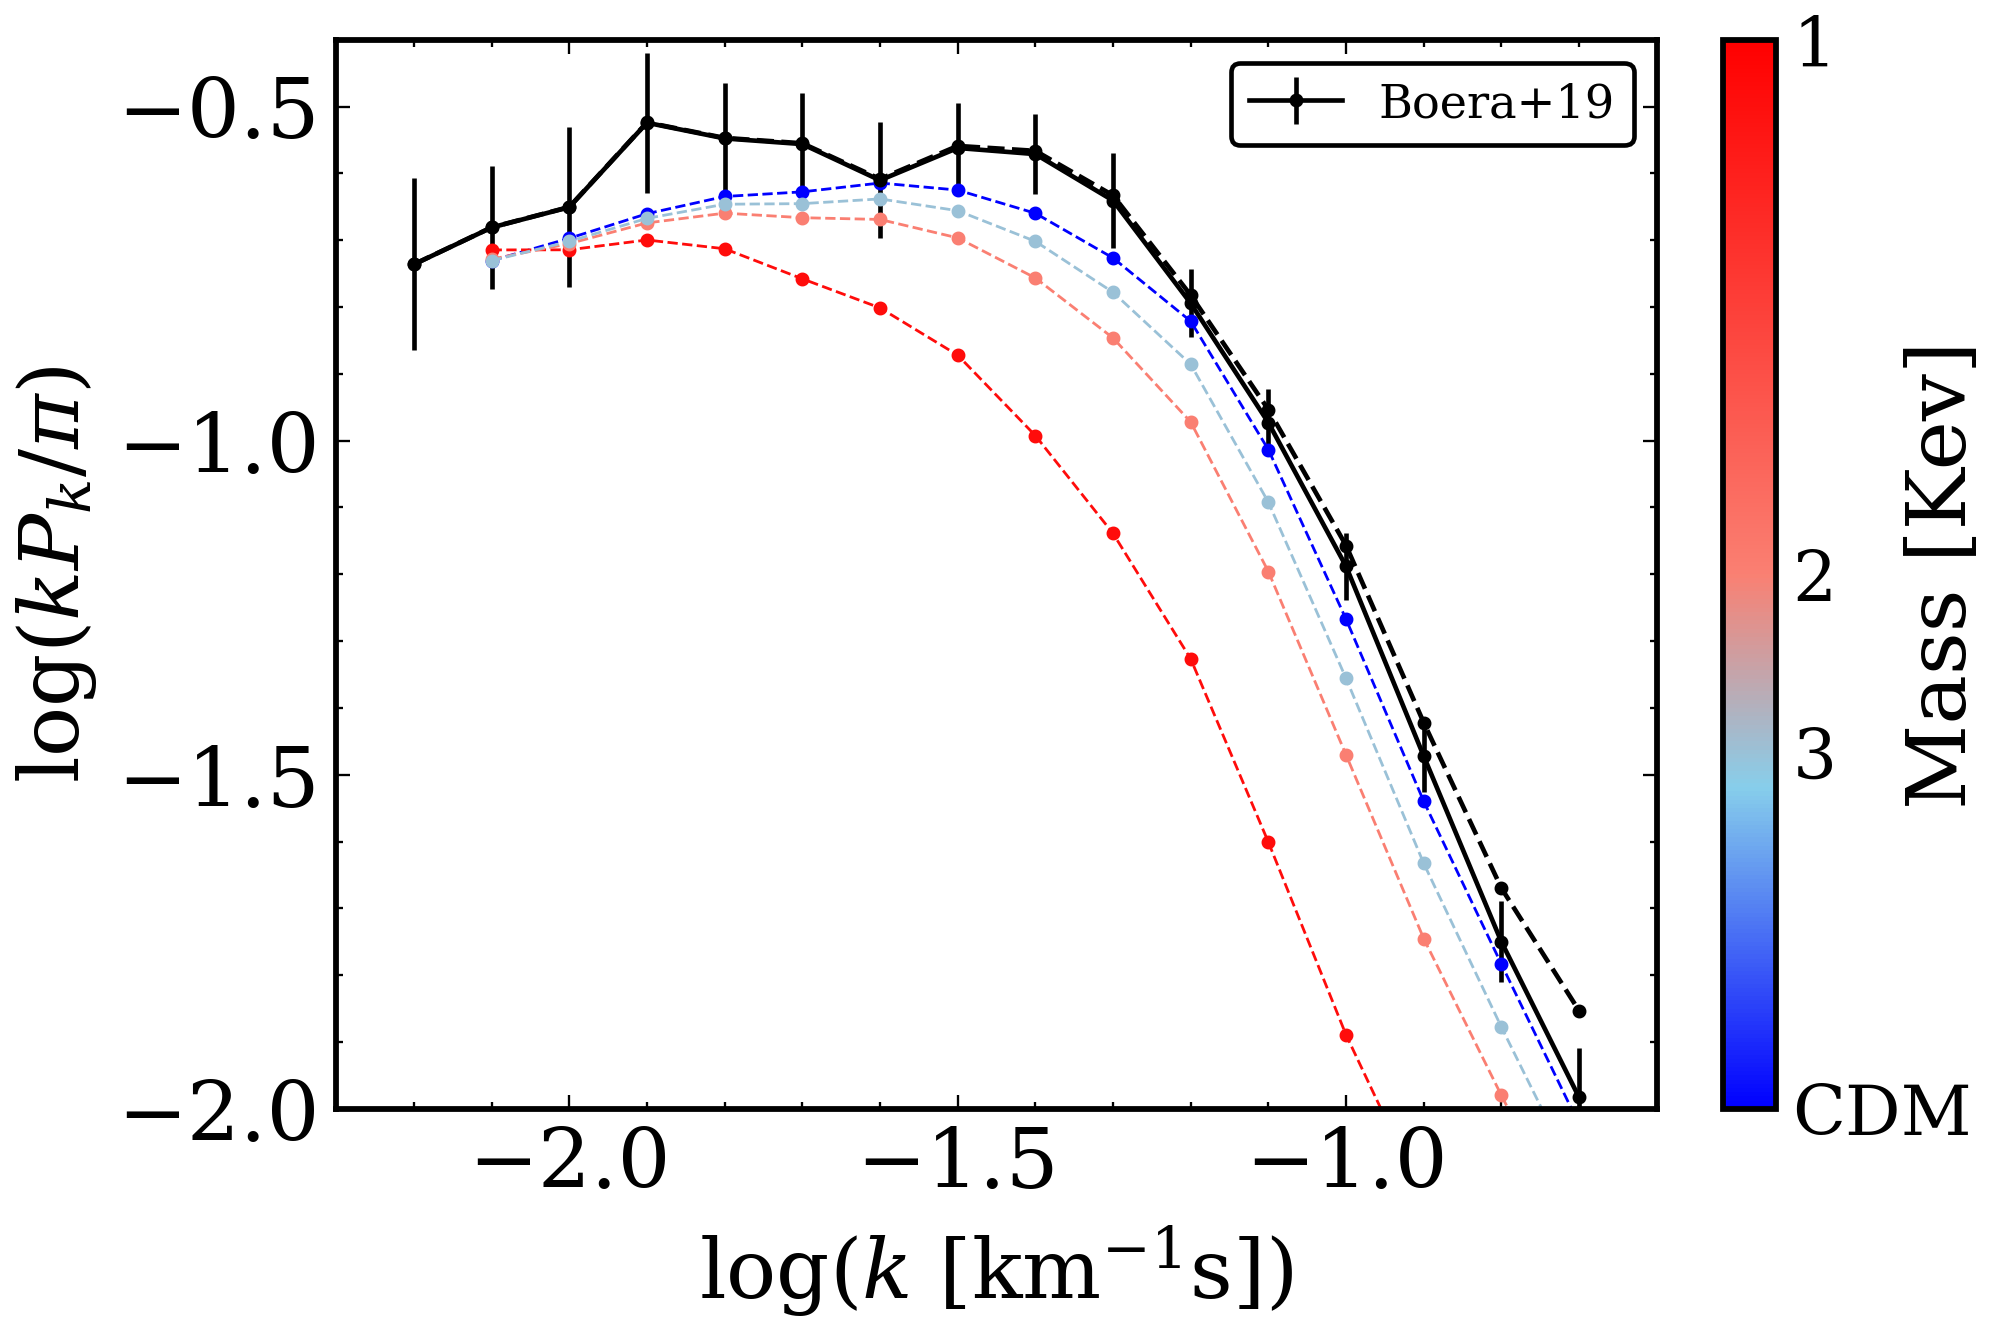
\includegraphics[width=0.99\textwidth]{img/ML/PS_sherwood.png}
        \caption{The Lyman-$\alpha$ flux power spectrum for different WDM models in the \texttt{SHERWOOD} simulation suite. For reference, we also plot the observed PS by \cite{Boera_2019}.}
        \label{fig: sherwood exact PS}     
\end{figure}


Since both the thermal state of the IGM and the WDM particle mass affect the Lyman-$\alpha$ forest, we could ask whether those two effects are degenerate. In fact, a hotter IGM means that the Voigt absoprtion profiles are wider, which smoothes out the forest at small scales, similarly to the effect how low WDM masses. If those two effects are completely degenerate, a smoother Lyman-$\alpha$ forest would not allow discriminating betweent a hotter IGM and a smalleer WDM particle mass. In Figure \ref{fig: PS thermal vs WDM} we show a comparison at $z=4.4$ of the effect of WDM models and thermal models within the \texttt{SHERWOOD THERMAL} suite on the Lyman-$\alpha$ flux power spectrum. Note that both effects are not completely degenerate. WDM models only suppress the power spectrum at small scales, while hotter models modify the power spectrum in the whole wavenumber range. As a consequence, the Lyman-$\alpha$ forest breaks the degeneracy between thermawl and WDM models.

\begin{figure}[ht]
        \centering
            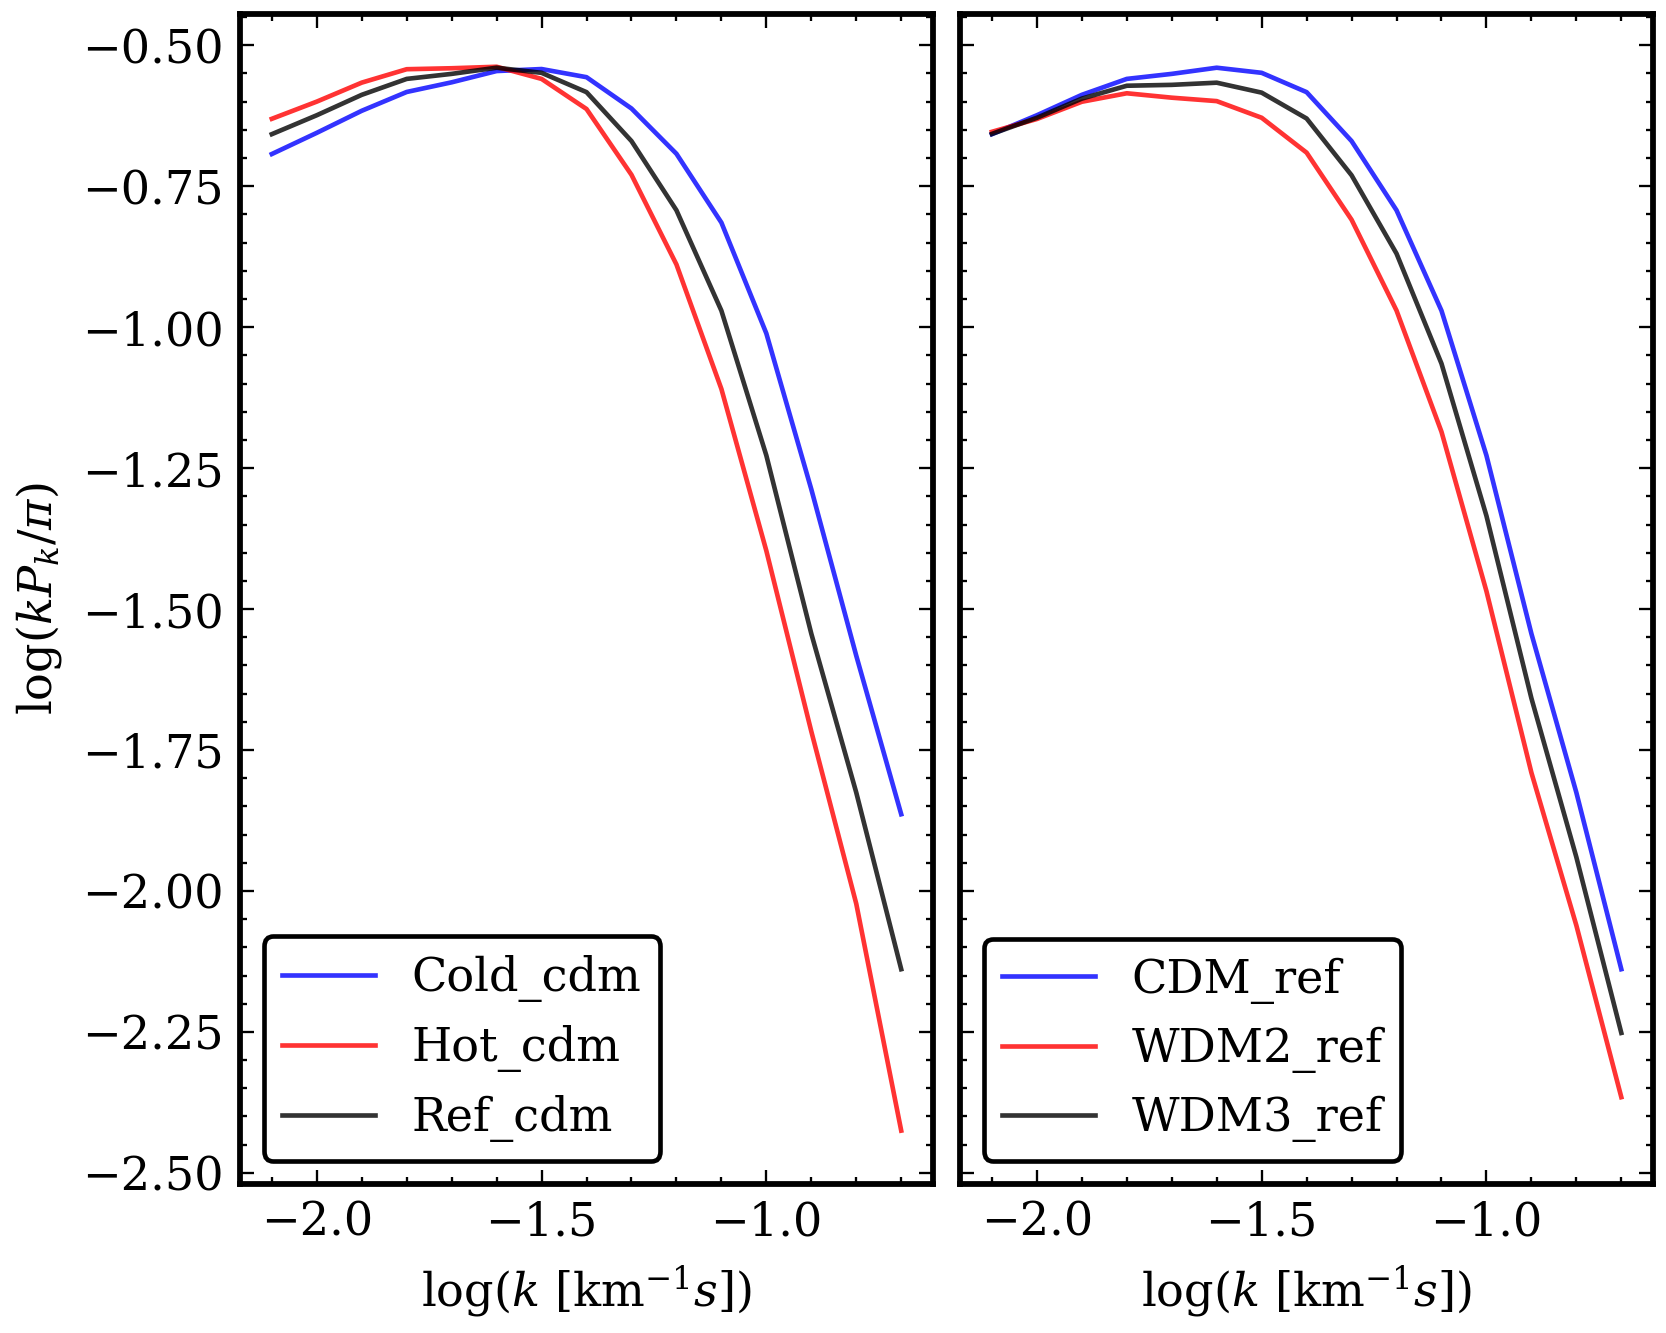
\includegraphics[width=0.8\textwidth]{img/ML/PS_thermal_vs_wdm.png}
            \caption{A comparison at $z=4.4$ of the effect of WDM models and thermal models within the \texttt{SHERWOOD} suite on the Lyman-$\alpha$ flux power spectrum. Note that both effects are not completely degenerate. WDM models only suppress the power spectrum at small scales, while hotter models modify the power spectrum in the whole wavenumber range.}
            \label{fig: PS thermal vs WDM}
\end{figure}   






\chapter{Deep Learning the Lyman-alpha forest}
\label{chap: deep learning}




\section{Introduction and motivation for the use of Deep Learning}
\label{sec:motiv_ml}


Fundamentally, a neural network is a directed and acyclic computational graph \cite{LeCun2015}. It represents a set of operations that transform input data input an output. In the simplest case of a fully connected network, the nodes of this graph are represented by neurons. Neurons are organized on successive layers, making the information flow from a layer to the following one. In the most basic scenario, the neurons in a given layer are linearly connected to the neurons in the previous layer. Each neuron then adds a bias to the result of the computation and applies a non-linear function to the result, which determines the activation state of the neuron. Consider the graph shown in \cref{fig:MLP}, where the input neuron has a value $x$ and the output neuron has a value $y(x)$. The intermediate layers have values
\begin{equation}
    \begin{dcases}
        x_1=\sigma(\alpha_1 x+\beta_1)\\
        x_2=\sigma(\alpha_2 x+\beta_2)
    \end{dcases},
\end{equation}
where $\alpha_i$ are the linear weights, $\beta_i$ the biases, and $\sigma$ is a non-linear activation function. Typical choices include $\tanh{}$ on ReLU (Rectifier Linear Unit) given by RELu$(x)=\max(0,x)$. Graphs such as the one shown in \cref{fig:MLP} as know as \emph{fully connected layers}. Much more complex architectures have of course been investigated. Depending on the specific problem and dataset, we can incorporate a priori knowledge of the problem in the design of the network. For instance, in Computer Vision, the use of \emph{convolutional layers} especially target at identifying key features in images has proven to be extremely successful \cite{CNN_rev}. In the analysis of time series, Long short-term memory (LSTM) neurons allow the network to ``remember" information from previous inputs \cite{LSTM_rev}. 




From the theoretical standpoint, neural networks are universal approximations (for sufficiently well-behaved functions), which makes them especially appealing in the modelling of complex systems. A concrete results is as follows \cite{universal_aprox}:

\begin{theorem}[Universal approximation theorem]\label{th:aprox}

    If $f\colon \mathbb{R}^n \to \mathbb{R}^m$ is a Lebesgue p-integrable function and $\varepsilon>0$, then there exists a fully connected ReLU network $F\colon \mathbb{R}^n \to \mathbb{R}^m$ such that
    $$
        \int_{\mathbf{R}^n}||f(x)-F(x) ||^p\ \differential x <\varepsilon.
    $$
\end{theorem}
Theorem \ref{th:aprox} can be expanded to include tight bounds on the depth or width of the network, which then depend on $n$ and $m$. Note that all the complexity of a fully connected neural network is generated by the non-linear activation function. With a linear activation function, a fully connected networks would be an affine transformation, which cannot approximate arbitrary non-linear functions.

\begin{figure}
    \centering
    \begin{subfigure}[b]{0.45\textwidth}
        \centering
                    \begin{tikzpicture}[scale=0.2]


                    \node (in) [circle, fill=white, draw=black, ultra thick, minimum size=1.3cm] {$x$};
                    
                    
                    \node (neu1) [circle, fill=orange, draw=black, ultra thick, below=of in , minimum size=1.3cm, xshift=2cm] {$x_1$};
                    
                    
                    \node (neu2) [circle, fill=orange, draw=black, ultra thick, below=of in , minimum size=1.3cm, xshift=-2cm] {$x_2$};
                    
                    
                    
                    \node (out) [circle, fill=dark-cyan, draw=black, ultra thick, below=of in , minimum size=1.3cm, yshift=-2cm] {$y(x)$};
                    
                    \draw [->,ultra thick] (in) -- (neu1);
                    \draw [->,ultra thick] (in) -- (neu2);
                    \draw [->,ultra thick] (neu1) -- (out);
                    \draw [->,ultra thick] (neu2) -- (out);
                    
                    \end{tikzpicture}
        \caption{Graph for a simple MLP with a hidden layer (in orange) and an output neuron (in cyan).}
        \label{fig:MLP}
    \end{subfigure}
    \hfill
    \begin{subfigure}[b]{0.45\textwidth}
        \centering
        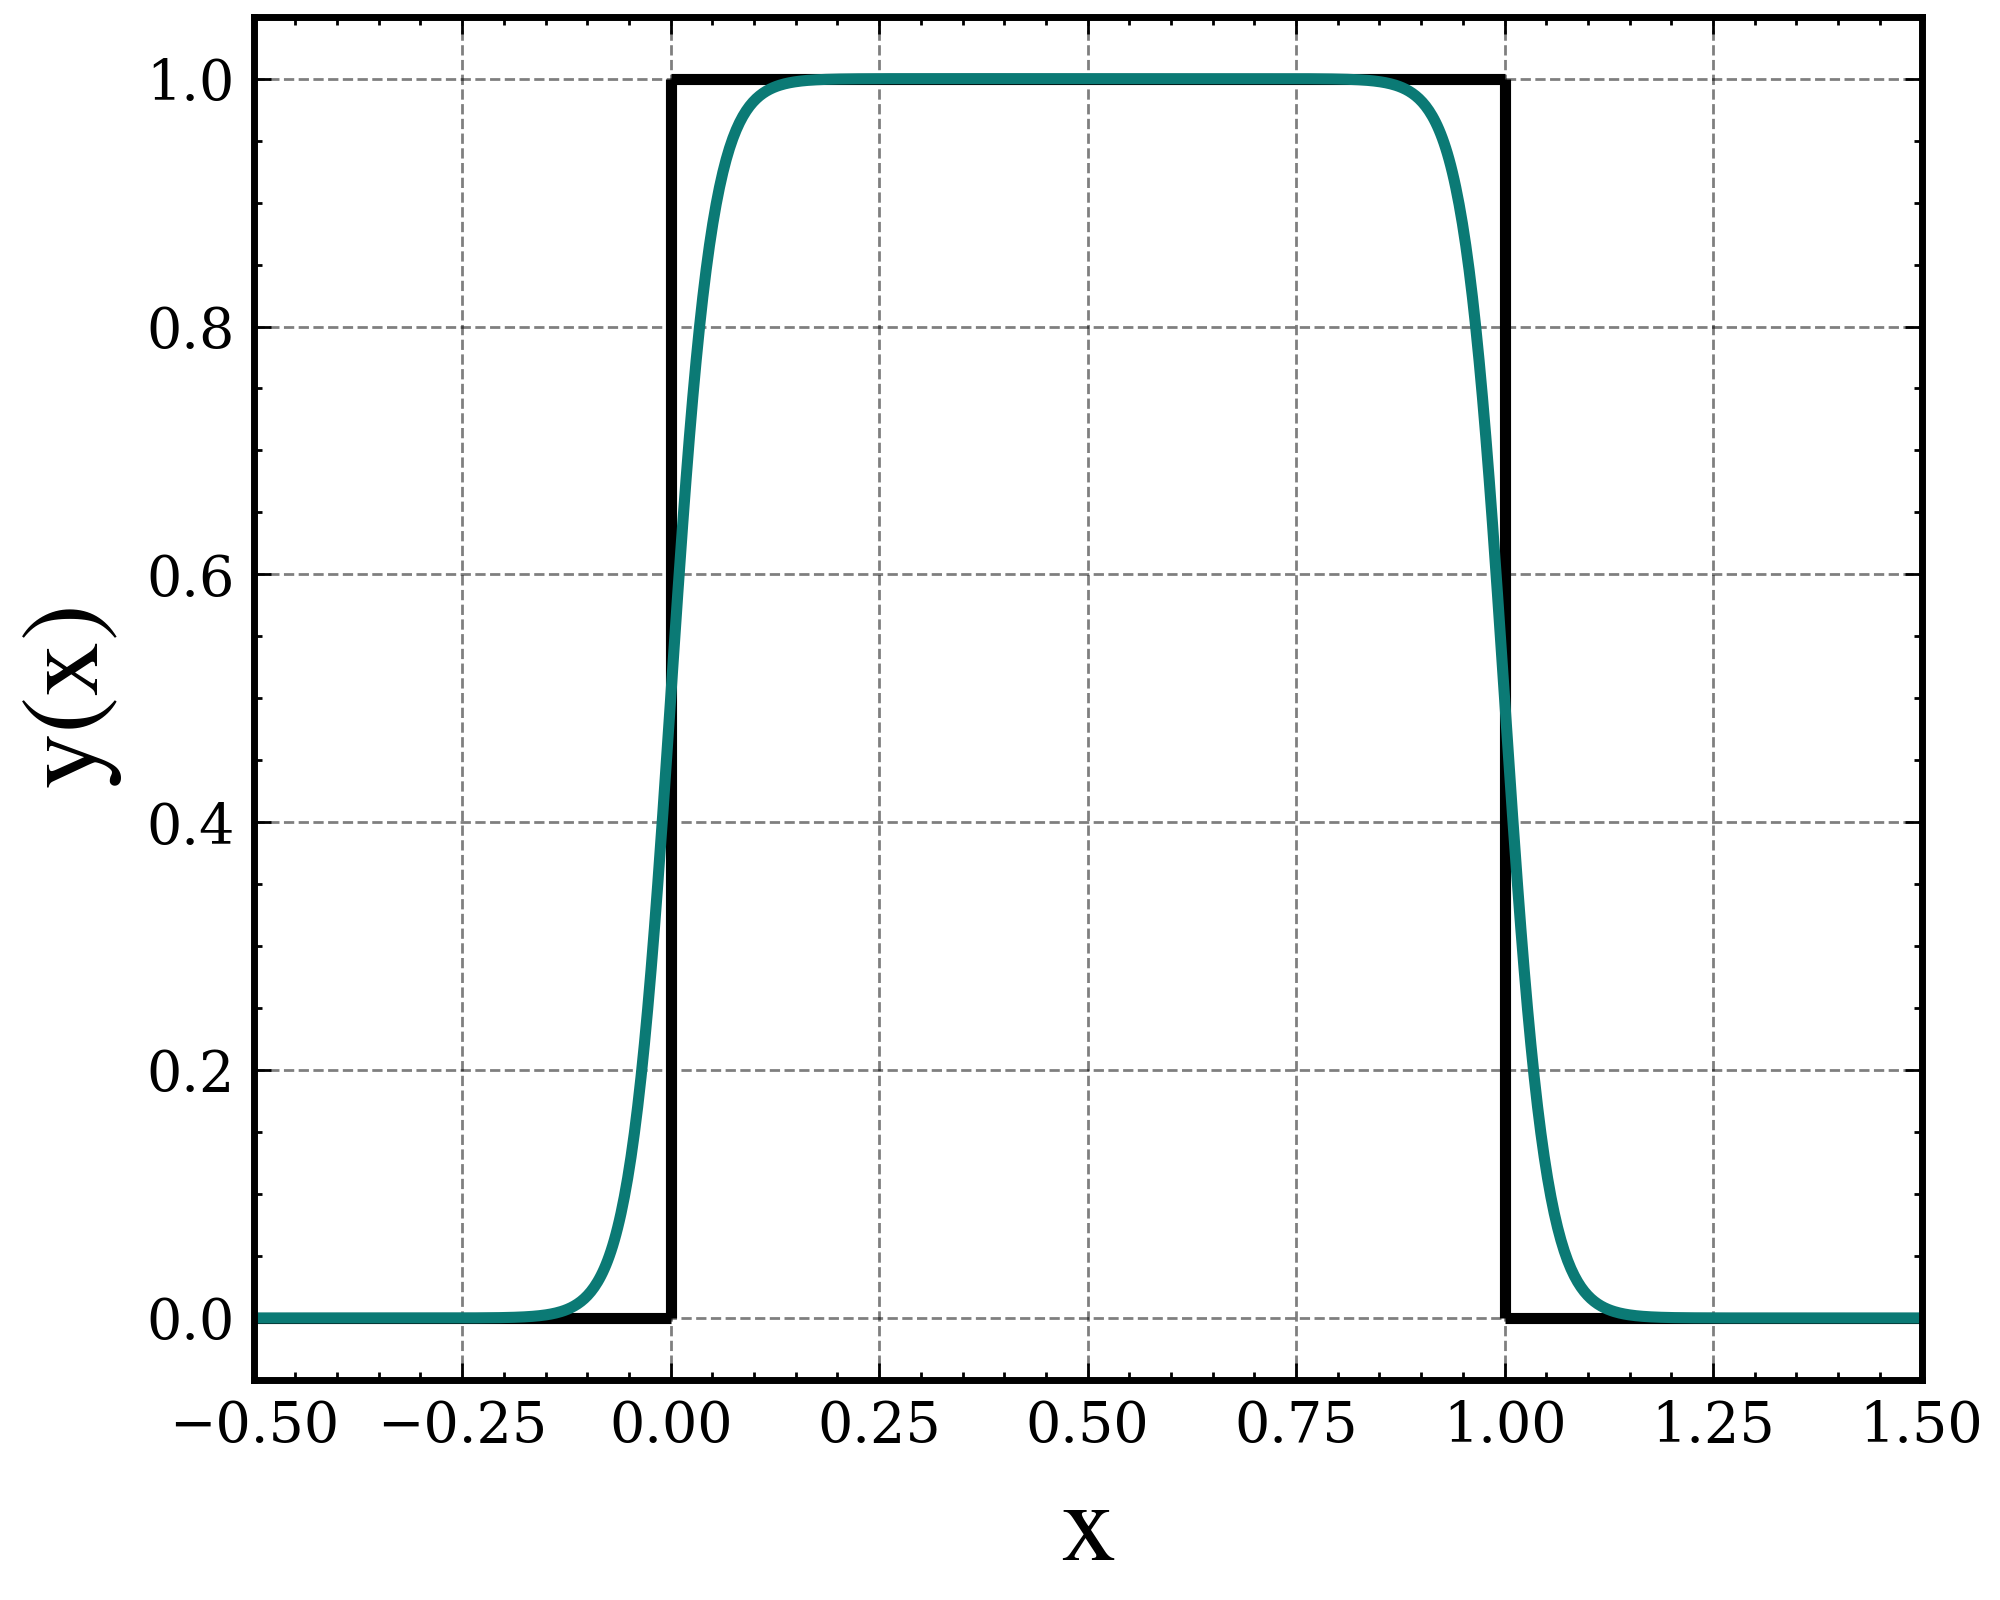
\includegraphics[width=1\textwidth]{img/ML/MLP_unit_impulse.png}
        \caption{Unit impulse (in black) and the output of the MLP shown in cyan approximating the impulse. }
        \label{fig:MLP_approx}
    \end{subfigure}
        \caption{A simple multilayer perceptron (MLP) with a single hidden layer and a $\tanh{}$ activation function is able to approximate a unit pulse function. From left to right and top to bottom, the three biases are $\{0, 20, 0\}$ and the four weights are $\{20, -20, 1/2, 1/2\}$.}
        \label{fig:ML MLP approx}
\end{figure}

This theoretical result can be easily visualized be understanding how a simple fully connected network (a multilayer perceptron, MLP) can approximate a unit impulse function. It is then enough to recall that a linear combinations of step functions can approximate any integrable function. In \cref{fig:MLP} we show a MLP consisting of an input neuron, and output neuron and a hidden layer with two neurons with a $\tanh{}$ activation function.
From left to right and top to bottom, we set the three biases as $\{0, 20, 0\}$ and the four weights as $\{20, -20, 1/2, 1/2\}$. The resulting MLP then produces the approximation shown in \cref{fig:MLP_approx} of the unit impulse over $[0,1]$. By expanding the number of neurons in the hidden layer we could approximate impulse functions of arbitrary width and height and centered at every arbitrary value. The high degree of expressivity of neural networks makes them particularly suited to parametrically approximate complex non-linear relationships between variables that would otherwise be intractable.

\begin{figure}
    \centering
    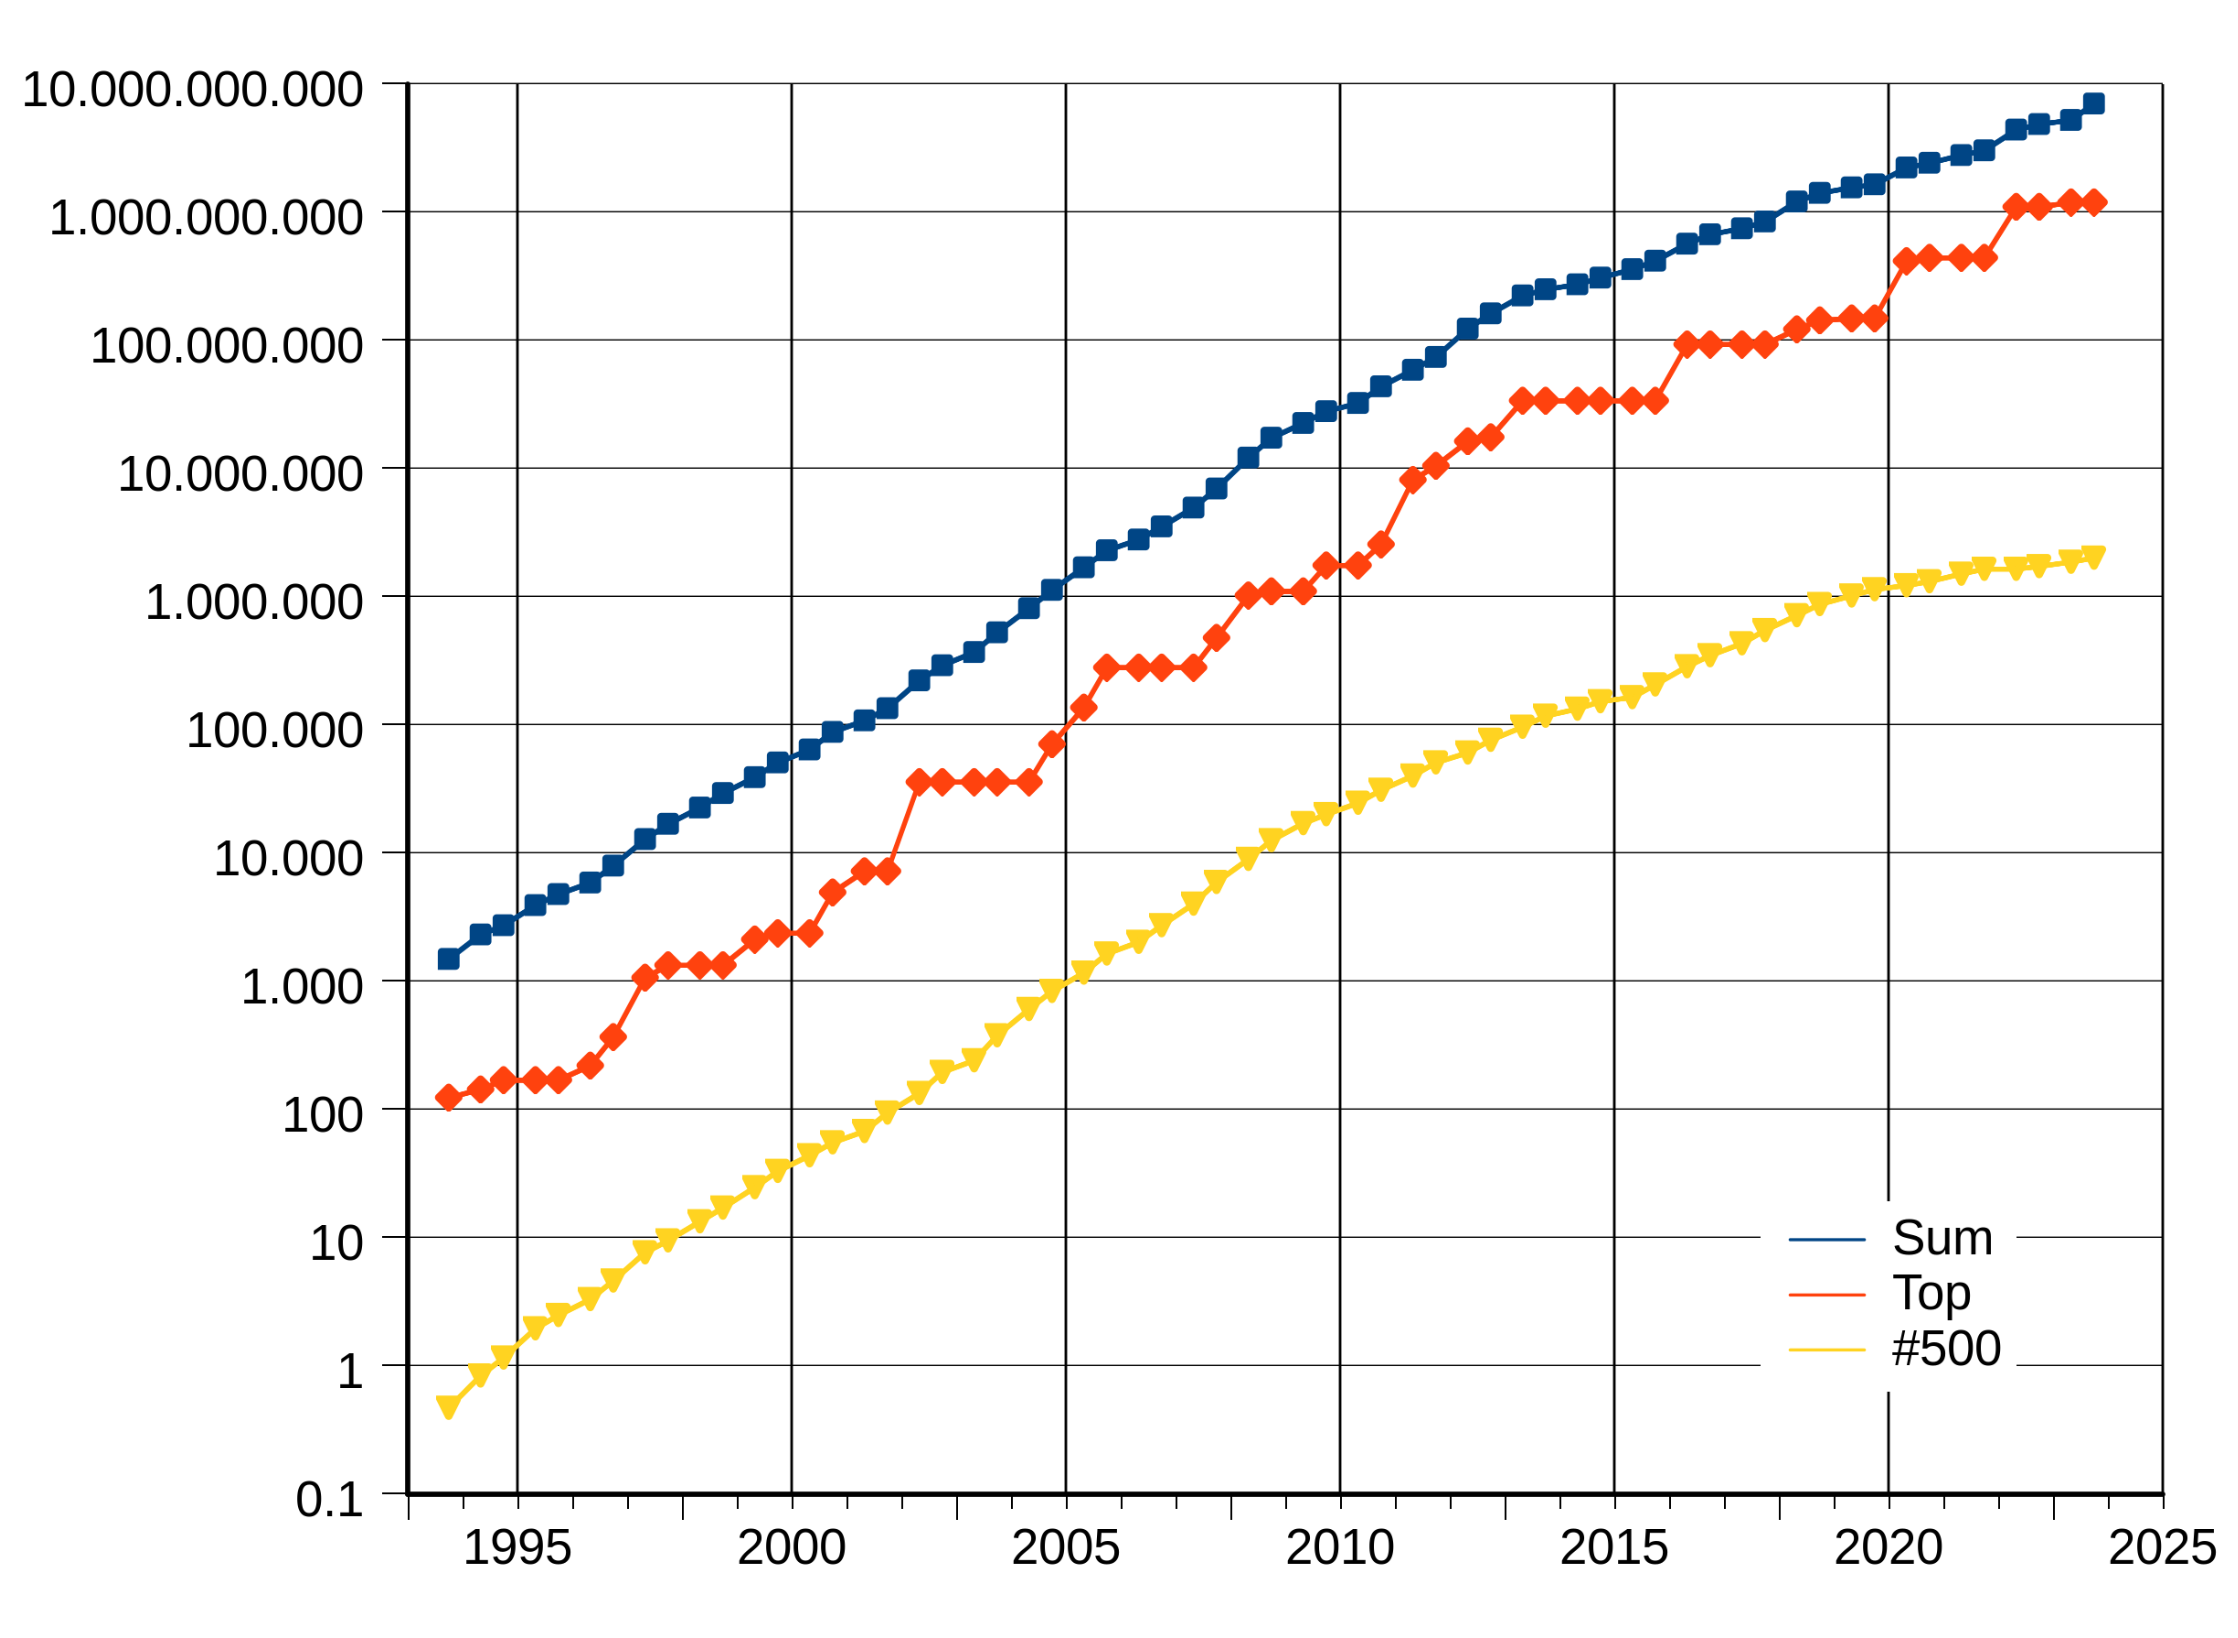
\includegraphics[width=0.7\linewidth]{img/ML/HPC.png}
    \caption{Evolution of the largest supercomputers in the \href{https://top500.org}{\textsc{TOP500}} list  in recent years (x-axis). The y-axis shows the peak performance in GFLOPS for the first-ranked computer (red), the last-ranked computer (yellow), and the cumulative power for the top-500 computers (blue). Source: \href{https://en.wikipedia.org/wiki/History_of_supercomputing}{Wikipedia}.}
    \label{fig:ML_HPC}
\end{figure}


Theorem \ref{th:aprox} establishes a theoretical aspect of neural networks supporting their utility, but it does not provide a method (nor does it guarantee the existence of any) to find networks that approximate a particular function of interest. The process of fitting a statistical model (such as a neural network) to a dataset of interest in know as \emph{supervised learning}, an constitutes one of the main aspect of this work, as we will explain in the rest if this section.
In recent years, the main points have allowed the rapid expansion of machine learning, marking a new era in the use of large parametric networks for real-world problems:

\begin{itemize}
    \item \textbf{Hardware development.} The rapid (quasi-exponential)growth in computer power in recent years, as exemplified by Moore's law \cite{Moor_law} means that extremely deep and complex models can now be trained and effectively used. As a reference, the language models \textsc{LLAMA} by Meta can have over 65 billion parameters \cite{Llama}. To handle this amount of data, High Performance Computing (HPC) infrastructures (such as supercomputers) are needed. Figure \ref{fig:ML_HPC} shows the rapid evolution for the top supercomputers in the world, as ranked by the TOP500 list\footnote{\url{https://top500.org}}. In 1993, the \textsc{Fujitsu Numerical Wind Tunnel} in Japan topped the list with 124 GFLOPS. In 2023, the list is topped by \textsc{Frontier} in the United States, with over 1000 PFLOPS, which corresponds to an 8000-fold improvement. Progress in hardware technology as also been remarkable. For instance, Graphics Processing Unit (GPU) are now common when training machine learning models. As a last example, in May 2017, Google introduced an architecture known as Tensor Processing Unit (TPU) especially designed to accelerate neural network operations \cite{TPU}. HPC also enables the generation of synthetic datasets from simulations, that can then be used as training datasets. We will leverage this idea in the rest of this work.


    \item \textbf{Computationally-efficient algorithms.} Together with hardware development, we have seen a rapid evolution of computational and mathematical algorithms in the field of statistical learning that have enabled the efficient utilization of HPC resources. The epitome of such algorithm might be \emph{backpropagation} \cite{backprop} which is the most common algorithm used in the training phase to update the weights when deploying a neural network. Together with backpropagation, a growing set of optimizers for deep learning problems have been developed. A popular choice is \textsc{Adam}, which was originally published in 2017 \cite{adam}.

    \item \textbf{Availability of large datasets.} The advent of next-generation instruments and data-collections systems provides the scientific community with increasingly large datasets. Prominent examples in the field of astronomy include Gaia \cite{gaia}, whose third data release (DR3) includes 10TB of data for 1.46 billion sources\footnote{\url{https://www.cosmos.esa.int/web/gaia/dr3}}, or the Euclid telescope, expected to deliver 850 GB of compressed data per day\footnote{\url{https://sci.esa.int/web/euclid/-/46661-mission-operations}}. At last, in \cref{fig:Supernovas_per_year} we show the evolution in the number of SNe discoveries per year. The figure as been obtained from \cite{SN_year}.



    
\end{itemize}

\begin{figure}
    \centering
    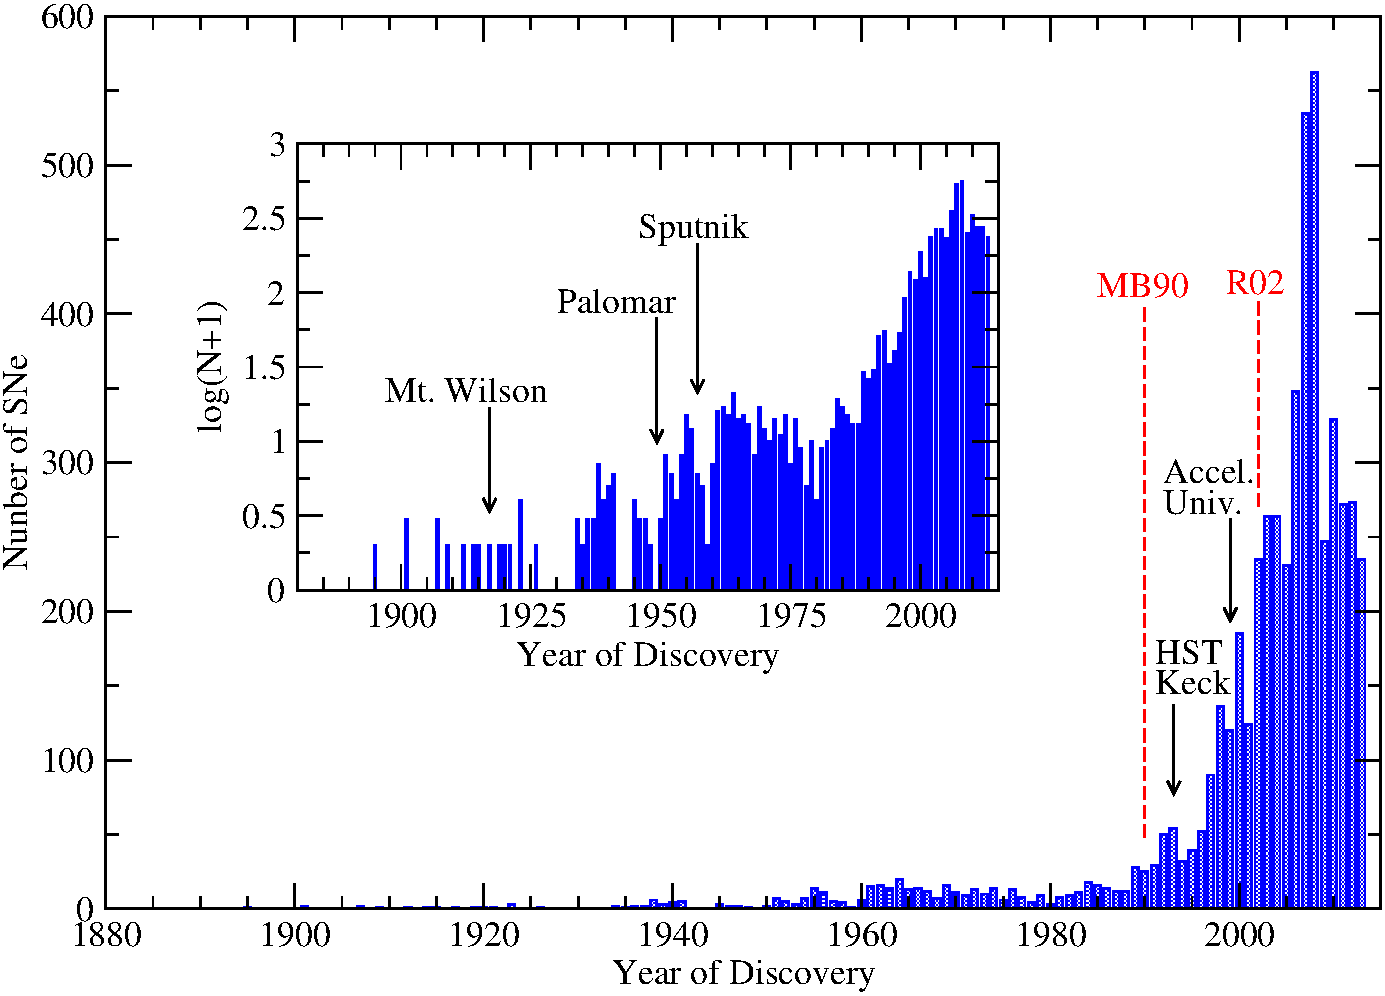
\includegraphics[width=0.7\linewidth]{img//ML/fig1_color.pdf}
    \caption{Histogram showing the number of SNe discovered each year as given by the Asiago Supernova Catalogue.}
    \label{fig:Supernovas_per_year}
\end{figure}



Let us demonstrate the relevance, pertinence, and range of applicability of machine learning methods in astronomy and cosmology by examining recent endeavours documented in the literature. While not exhaustive, this examination provides a broad overview of previous efforts in the field, and illustrates some recent successes of machine learning-oriented approaches in data-driven problems.
\par
The abundance of data from surveys covering large regions of the sky aimed at targeting QSOs makes supervised statistical techniques a particularly attractive data analysis technique. For reference, the main quasar sample in the data release number 16 for the Extended Baryon Oscillation Spectroscopic Survey (eBOSS) contains 434820 targets with redshifts in the range $0.8<z<2.2$ \cite{eboss}. The prediction of the intrinsic Lyman-$\alpha$ emission line from high redshift QSOs is a non-trivial problem that has important implication in the study of IGM damping wings and the reionization of the later \cite{MiraldaEscude_IGM}. Reconstruction techniques often rely on the correlation of the Lyman-$\alpha$ peak with other observable lines and information redward of the Lyman-$\alpha$ line. Machine learning approaches are then suitable to connect the unattenuated information redward of the Lyman-$\alpha$ peak with its intrinsic profile. In \citetitle{qso_challenge} \cite{qso_challenge}, the authors perform an in-depth comparison of different state-of-the-art techniques based on statistical learning. The authors blindly evaluate their performance on two QSOs samples randomly extracted from X-Shooter and BOSS with $3.5<z<4.5$, in such a way that selecting samples already used in the training data-set was avoided. The various techniques range from principal component analysis (PCA) approaches, such as \cite{Bosman2021_pca}, to deep learning networks \cite{Liu2021}. The authors conclude that the better performing pipelines consistently rely on machine learning approaches. The authors caution against overreliance on machine learning techniques due to their potential lack of statistical uncertainty, which is one of the main aspect that we will develop in this work.


\par
Parameter inference on WDM using deep learning has already been tentatively explored in the recent literature.
The paper \citetitle{wdm_from_field} \cite{wdm_from_field}, which is especially relevant for this work, demonstrates that neural networks can be used to recovered WDM parameters from observed field density images. The authors present a suite of 1500 cosmological N-body simulations with varied WDM mass in the range 2.5 to 30 KeV. Field density images of size 25h$^{-1}$Mpc, with varied image resolution, simulation resolution and redshift (in the range $0\leq z \leq 5$) are extracted from the simulation runs. The images are augmented usual standard techniques (such as image rotation) and then incorporated into training datasets. The authors use a Convolutional Neural Network (CNN) trained to directly predict WDM masses based on an input density field image. Their fiducial convolutional network trained with the set of highest resolution image is able to accurately recover WDM masses with an accuracy of $\pm$1 KeV for models up to 10 KeV. After this threshold value, the network is no longer able to recover the true mass as predicts an approximately constant mass, see \cref{fig:ML paper wdm field}. Note that in the architecture presented by the authors, the network is also trained to predict an uncertainty estimate. Another interesting insight offered by this paper refers by the capacity of neural network to make use of the full information contained on a field distribution (in this case, the density field). By training a network on a full density field image the models learns the relevant properties of the field that can lead to an accurate parameter prediction. The authors train another model only on summary statistic, in particular, on the density power spectrum, and compare its performance with their fiducial model trained on the full images. The model trained only on the power spectra shows a significantly degraded performance, with higher uncertainties and accurate prediction only up to 5.5 KeV. This illustrate how deep learning techniques can help harvesting the full information present in a field (or generally, in a complex input tensor).


\begin{figure}
    \centering
    \begin{subfigure}[b]{0.53\textwidth}
        \centering
            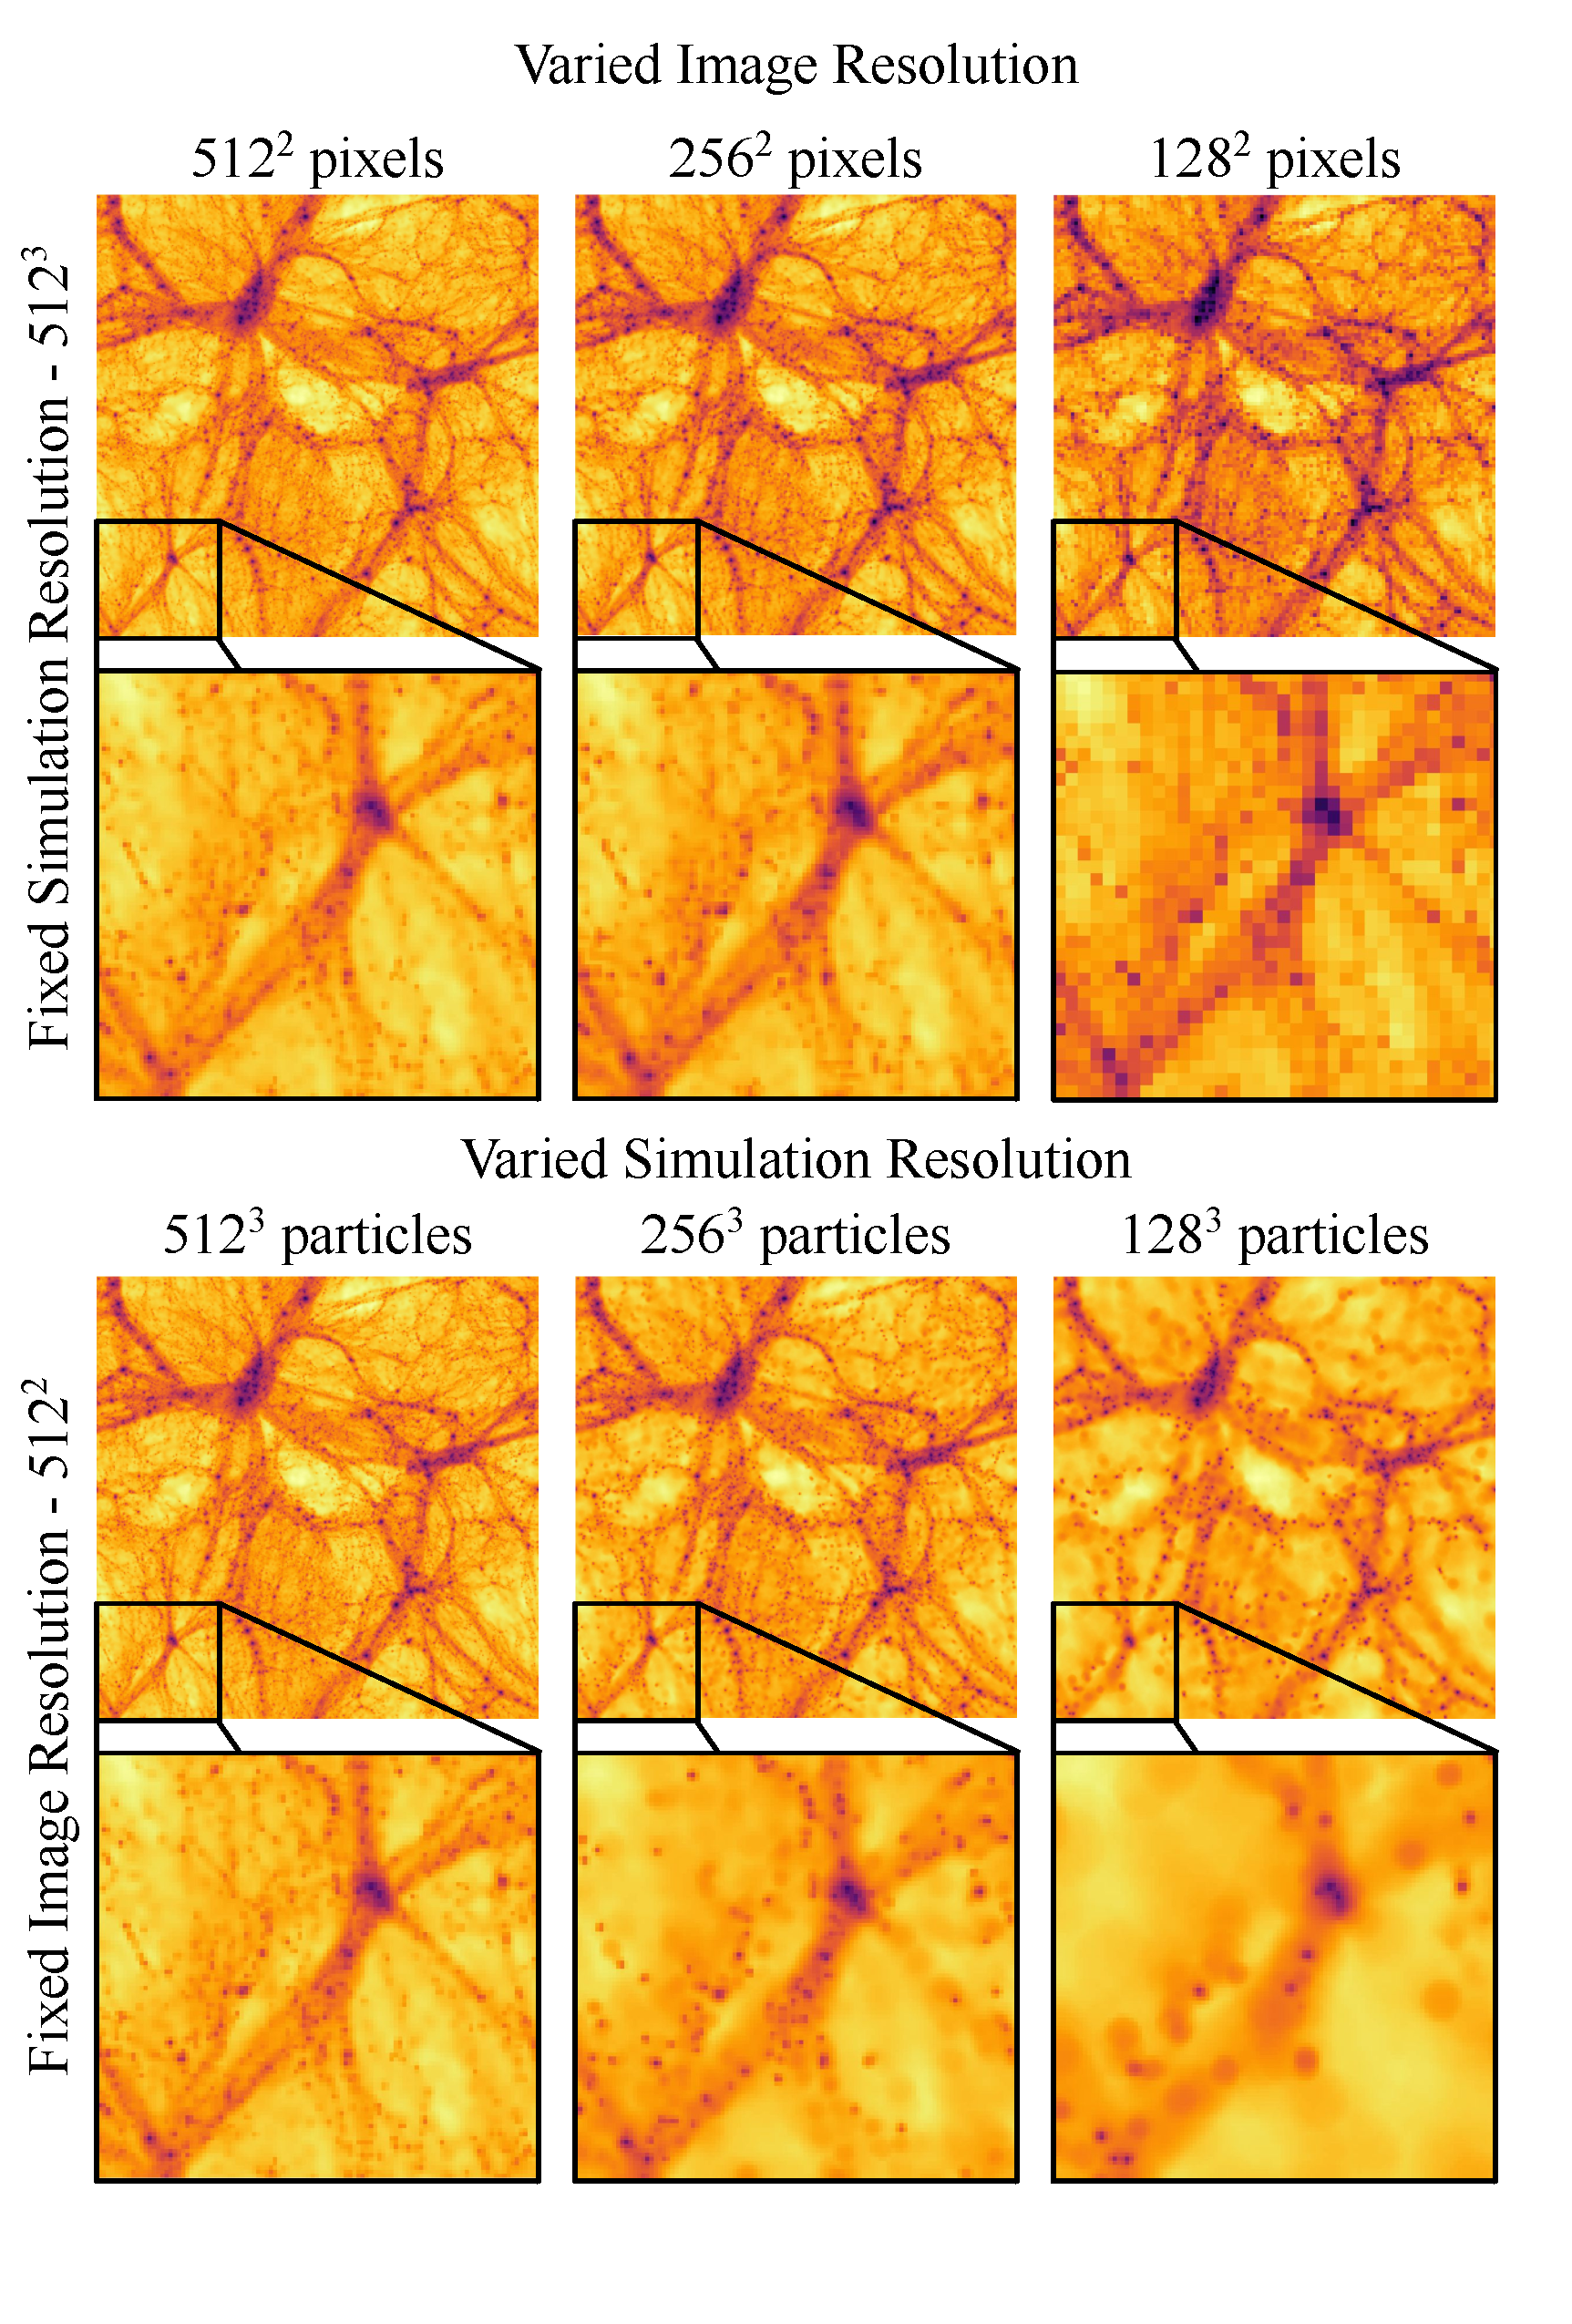
\includegraphics[width=1\textwidth, trim={0 22.2cm 0 0},clip]{img/ML/CAMELS_Images_Update.pdf}
    
    \end{subfigure}
    \hfill
    \begin{subfigure}[b]{0.45\textwidth}
        \centering
        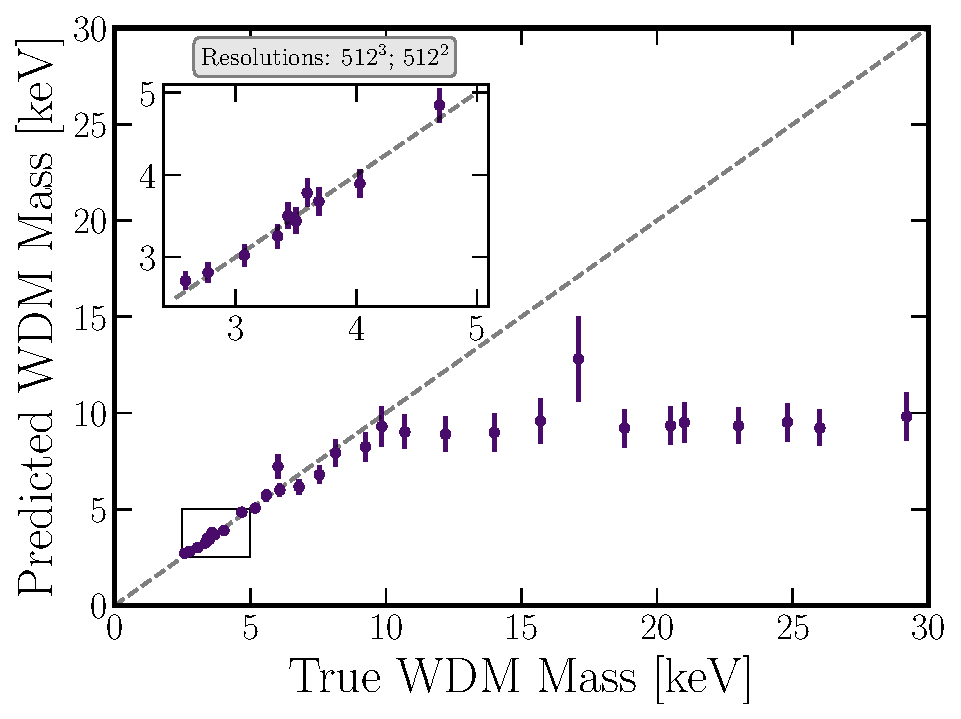
\includegraphics[width=1\textwidth]{img/ML/results_fixed_sim512_res512_z0.pdf}     
    \end{subfigure}
        \caption{Figure extracted from \cite{wdm_from_field}. The left panel shows a sample image density field used in the training data by the authors, with varied image resolution. The right panel shows a sample a predicted WDM masses versus the true WDM mass of the simulation for their fiducial neural network, which can accurately recover the WDM model within a 1 KeV accuracy up to 10 KeV.}
        \label{fig:ML paper wdm field}
\end{figure}

Another recent use of deep learning to analyse IGM data can be found in the paper \citetitle{lynna} \cite{lynna}, where authors harvest the field level potential of residual convolutional networks to perform inference on the thermal parameters of the IGM, namely $T_0$, the temperature at mean density, and $\gamma$, the slope of the temperature-density relation. Their model is trained on simulation boxes with side-length 120 Mpc from which $10^5$ sightlines are extracted and processed to produce mock Lyman-$\alpha$ spectra. The simulation boxes are run with different thermal parameters, by sampling 121 $(T_0,\gamma)$ combinations in the parameter space. The network is trained on 24000 labeled spectra from the mix of thermal models, and the architecture is designed to predict a mean value for the thermal parameters as well as an estimate for the parameter covariance matrix. Figure \ref{fig:ML LYNNA} shows the scatter in the point predictions for $(T_0,\gamma)$ for a set of 4000 unseen test spectra. The true parameter values, shown as dashed lines, are recovered by the average of the point predictions, shown as the dark green cross. The authors also perform a comparison with an inference pipeline based on the traditional transmitted flux power spectrum, and find that the posterior constraint using the machine learning field-level approach are 5.65 times tighter.


\begin{figure}
    \centering
    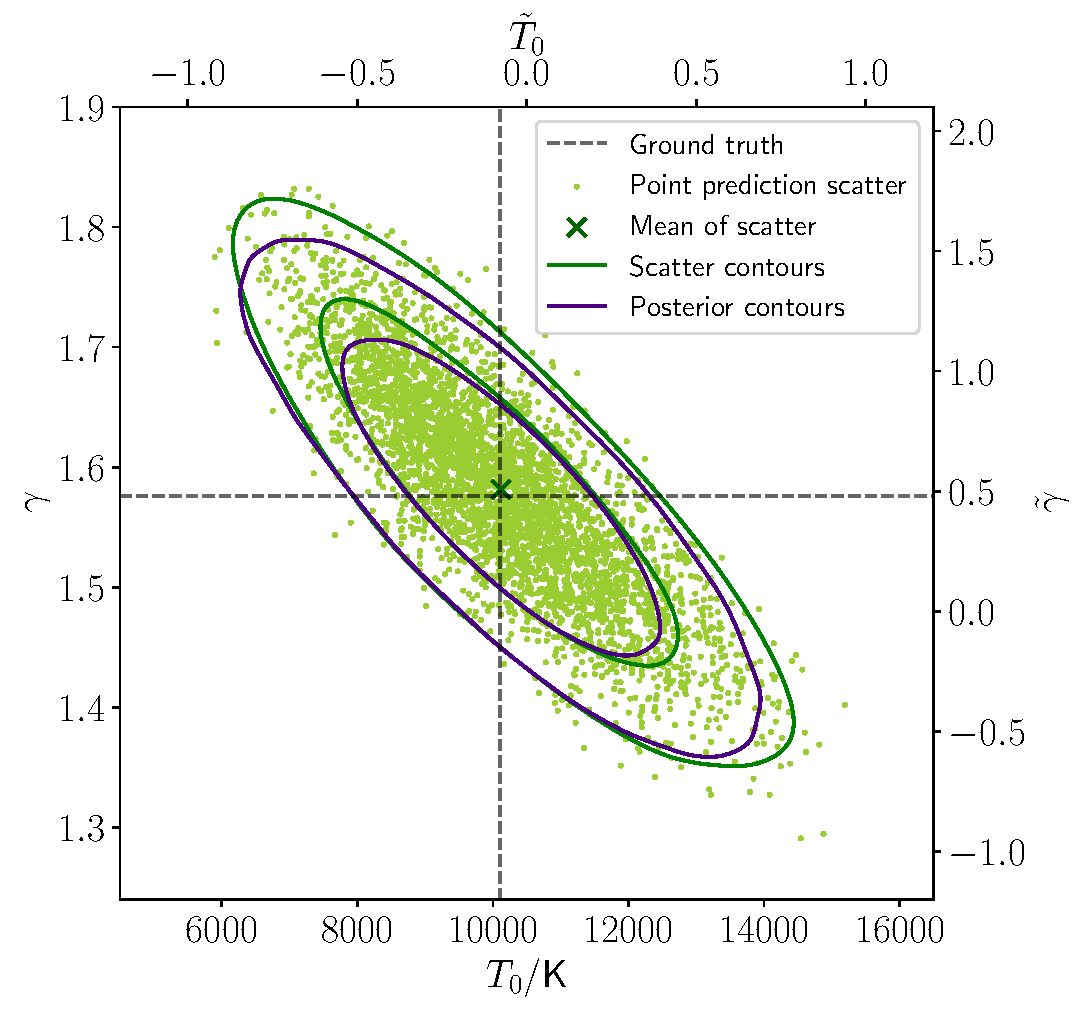
\includegraphics[width=0.6\linewidth]{img//ML/scatter__and__posterior_contours_fiducial_tdr.pdf}
    \caption{Figure extract from \cite{lynna} showing the performance of the neural network recovering thermal parameters on a set of unseen skewers. The true parameter values, shown as dashed lines, are recovered by the average of the point predictions, shown as the dark green cross.}
    \label{fig:ML LYNNA}
\end{figure}






\section{Fundamentals of (Bayesian) Neural Networks}

A very general regression problem in statistical learning \cite{James2021} arises when we observe a quantity $Y$ that is assumed to depend on an independent variable $X$ through a relation of the form

\begin{equation}
    Y = f(X)+\mathcal{N}(0,\sigma),
\end{equation}
where $f$ is a function defining the relation $Y=Y(X)$ and $\mathcal{N}(0,\sigma)$ is an error term modeling a zero-mean Gaussian noise. The problem then consists of estimating $f$ given a sample of observations $\{ X_i, Y_i\}_i$ to obtain a functional form $\hat{f}$ that can then be evaluated to obtain predictions. Following the examples in section $\ref{sec:motiv_ml}$, $X$ might be the flux spectra redward of the Lyman$-\alpha$ peak, and $Y$ might then be the intrinsic shape of the Lyman$-\alpha$ peak in the quasar spectra. The noise then is produced by different sources, for instance, associated with the instrumental devices. We could then use the obtained $\hat{f}$ to predict to intrinsic Lyman$-\alpha$ peak of a QSO, $\hat{f}(X)$, when we only have information about the spectrum redward of it, $X$. As it is expected, the quality of our prediction depends on how accurate is the approximation $\hat{f}$ with respect to $f$, but also on how noisy our data is. In fact, we see that, if the true quantity associated with $X$ is $Y$:

$$(Y-\hat{f}(X))^2=(f(x)+\mathcal{N}(0,\sigma)-\hat{f}(X))^2.$$
Taking expected values and noting that the only stochastic component here is the noise, we obtain 
\begin{equation}\label{eq:var_noise_model}
    \mathbb{E}[(Y-\hat{f}(X))^2]=(f(X)-\hat{f}(X))^2+\sigma^2.
\end{equation}
In \cref{eq:var_noise_model}, the first term of the right-hand side represents the error produced by approximating $f$ by $\hat{f}$, while the second term is a theoretical limit imposed by the noise properties.

Parametric methods represent a powerful statistical learning tool to approximate the target relation $f$ between variables.
Methods such as linear regression, which approximates $Y=f(X)$ using a linear functional form on the parameter values, offer limited flexibility in terms of approximating complex relations but allow for a high degree of interpretability of the model. On the other end of the spectrum, deep learning models offer a large degree of expressivity (see \ref{sec:motiv_ml}), but interpretation of individual parameters is often not possible. Increasing the number of parameters can also cause the model to learn from spurious structures in the finite data sample, or the learn from possible noise correlation. This process, known as \emph{over-fitting}, can significantly impact the predictive performance of the model when predicting on unseen data. Multiple techniques have been explored to mitigate over-fitting \cite{overfitting}, we will adopt some of them in this work and explain them in the following sections.

In this section we will discuss the basic workflow involving a deep learning model in a general and abstract scenario. We will restrict ourselves to the topics that are relevant for this work, and later explain in detail how we implement this workflow for our problem.
The general workflow when working with a deep learning statistical model under supervised learning includes the following phases:
\begin{enumerate}
    \item Collecting/data and processing it to generate a training dataset. This requires specific domain expertise to assess the quality and representability of the data.
    \item Designing a deep learning architecture, i.e., a computational graph that depends on a set of parameters and that generates target outputs from the input data.
    \item Using the available data to train the model. This is done by optimizing the model parameters by minimizing a selected loss function.
    \item Assessing the performance of the network a validation dataset, previously unseen.
    \item Using the model on real unseen data to make predictions.
\end{enumerate}

\subsection{Dataset generation, data augmentation and overfitting.}\label{sec: dataset}

In a general real-world setting only a finite dataset is available to us, for instance, obtained from observational procedures.
That is, we have a set of pairs $\mathcal{D}=\{X_i,Y_i \}_{i=1}^{i=N}$ of $N$ observations from an input-output pairs, distributed according to some distribution $F(X,Y)$:
\begin{equation}
    (X_i,Y_i) \sim F, i=1,...,N.
\end{equation}
Of course in general, we don't have access to the distribution of this population (i.e., the function $f$ describing the data relation $Y=f(X)$), otherwise we would already have a perfectly accurate model, and we would not to invoke any statistical learning tool.
The challenge is then to use our sample $\mathcal{D}$ to infer properties of the population.
Since we don't have access to the generating function $f$, we cannot assess the general performance of the model on arbitrary input data.
For this purpose, the training dataset $\mathcal{D}$ is typically split into two disjoint subsets $\mathcal{D}=\mathcal{D}_T \sqcup \mathcal{D}_V$, where $\mathcal{D}_T$ represents the subset of the data used for training, and $\mathcal{D}_V$ represents the subset of the data used to validate the model and assess its performance.
The central idea behind this split is to be able to validate the model on data that has not been used in the training process, allowing for an estimation of the model's generalization to the population given by:
\begin{equation}\label{eq_ch3:global_loss}
    \varepsilon =\mathbb{E}_F[\mathcal{L}(Y,\hat{f}(X|\mathcal{D}_T))],
\end{equation}
where $\mathcal{L}$ is a loss function.
The exact form in which the $\mathcal{D}$ is split needs chosen a priori, with the aim of having a representative sample of the population.
A common easy-to-implement strategy is to randomly select the samples in $\mathcal{D}$ that will be part of $\mathcal{D}_V$ and distributing them according to a ratio, that is commonly taken to in the range $60-80\%$, meaning that a larger percentage of $\mathcal{D}$ is dedicated to training.
In this case, an unbiased estimator of $\varepsilon$ is
\begin{equation}
    \hat{\varepsilon}=\frac{1}{|\mathcal{D}_V|}\sum_{i=1}^{|\mathcal{D}_V|}\mathcal{L}(Y_i,\hat{f}(X_i)),
\end{equation}
where the sum runs over the validation dataset.
More complex strategies that take into account the topology of the data exist and allow for an optimal training-valiation split \cite{data_split}. 
The validation subset can also be sequentially cycled through all the available samples in a series of methods called \emph{cross-validation} \cite{cross_validation}. Cross-validation uses all available data in a validation stage by retraining a model on different disjoint splits of the data. This allows for a more precise evaluation of the model.

If the training subset $\mathcal{D}_T$ is not representative of the population, then the global error in \cref{eq_ch3:global_loss} will be large, and the model will not be able to learn the general properties of the data.
This can cause the model to overfit and learn from spurious correlation in the data and noise, and can be encouraged by having an excessive number of free parameters.
Overfitting is not an intrinsic characteristic of deep-learning models, can can also be seen for instance in simple polynomial regression when the number of ``independent'' points exceeds the order of the fitting polynomial.
Figure \ref{fig:ML overfit poly} illustrates the simple example of polynomial regression overfitting the training dataset as the order of the polynomial increases. Note how, by construction, the fit becomes increasingly accurate on the training data, but looses generalization power on unseen points.
\begin{figure}
    \centering
    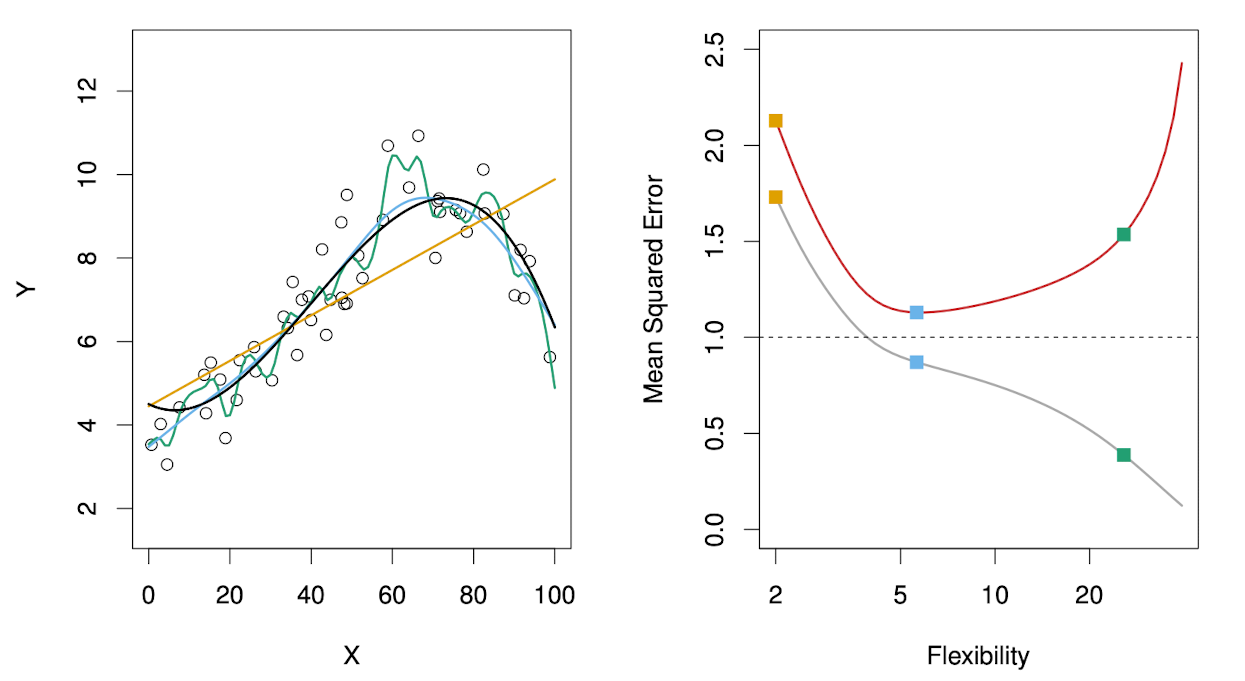
\includegraphics[width=0.7\linewidth]{img/ML/poly_overfit.png}
    \caption{The left panel shows the data points (with added noise) generated from a function $f$ in black. Three generative polynomial models are fitted to the data: linear regression in orange, and two smoothing splines in red and blue. The right panel shows the fitting error as a function of the polynomial degree, i.e., the flexibility of the model. The gray curve shows the error on the training dataset, which is monotonically decreasing. The red curve shows the error on the validation dataset, which initially decreases but then grows as the model overfits the training data. Figure extracted from \cite{James2021}. }
    \label{fig:ML overfit poly}
\end{figure}

The training data $\mathcal{D}_T$ can be artificially extended using \emph{data augmentation} techniques \cite{data_augmentation} to generate new training points from existing points. Data augmentation aims at presenting the model with data that maintains intrinsic properties of the original data but varies other features that should not affect the prediction. This approach can be understood to be inspired by symmetry considerations\footnote{A strawberry is a strawberry regardless of its orientation} and is particularly useful in computer vision tasks. Some common data augmentation techniques for image processing include:

\begin{itemize}
    \item Basic geometric transformations such as rotation, translation or flipping an image (or field) are efficiently implemented. Cropping can also be easily implemented, but changes the dimensionality of the data.
    \item Basic color space manipulation in colored images, including isolating a single color channel, or modifying the brightness of an image.
    \item Noise injection during training is particularly useful in making neural networks robust against noisy and corrupted data. Note that this can be relevant if the data we are expecting to use the trained model on has noisy (for example instrumental data from a spectrograph). The noise can be randomly drawn from independent distributions, or drawn from a noise model if we have additional insights on how to model it.
    \item Convolutional operations with kernels, such as the Gaussian kernel to apply a limited spatial resolution (blurring), or the Sobel kernel for related to edge detection.
\end{itemize}


\subsection{Deep learning architecture}\label{sec:deep learning archi}
The network architecture defines the parametrization of the function that approximates the true underlying relation between input and output data points. In this section we briefly explore some basic building blocks used when constructing a deep learning network.
A neural network (NN) $\phi$ is a computational graph with an input tensor $X$ and an output tensor $Y$ and parametrized by a set of values $\omega$ that define a functional model
\begin{equation}
    Y=\phi(X|\omega)\equiv \phi_\omega (X).
\end{equation}
For simple linear topologies a NN can be specified given a set of connected \emph{layers} that carry out the elementary operations. These layers can be grouped in \emph{blocks} to form subnetworks inside a NN. Three of the simplest layer architectures are \emph{feedforward} layers (also known as \emph{dense} layers), convolutional layers, and residual layers. Since they will be of use in our machine learning workflow, we will discuss their exact structure.

\begin{itemize}
    \item In the simplest feedforward network, such as the one illustrated in \cref{fig:MLP}, all layers are linearly connected with an additional activation function, leading to a model of the form

    \begin{equation}
        \begin{aligned}
            &X=\boldsymbol{l}_{0}, \\
            &\boldsymbol{l}_{i}=s_{i}(\boldsymbol{W}_{i}\boldsymbol{l}_{i-1}+\boldsymbol{b}_{i})\quad\forall i\in[1,N], \\
            &Y=\boldsymbol{l}_{N},
        \end{aligned}
    \end{equation}
    where $l_i$ are the layers, $W_i$ the weights, $b_i$ the biases, $\sigma_i$ the activation functions and $N$ the number of layers.
    
    
    \item Convolutional layers are especially useful in signal processing and computer vision problem. They incorporate multiple convolution operations on the input array. The parameters of the layers define the exact way the convolution is performed. Consider for illustration purposes the case of an input 2D array of size $(N,N)$. The convolutional layer is internally parametrized by a kernel $\omega$ of shape $(m,m)$ such that the input $X$ to the layer is transformed as
    \begin{equation}
        Y_{i,j}=\sum_{a=0}^{m-1} \sum_{b=0}^{m-1} \omega_{ab} X_{i+a,j+b}.
    \end{equation}
    The output size will be $(N-m+1,N-m+1)$. Lastly, a user-specified non-linearity is applied. The implementation of convolutional layers in machine learning APIs is usually done by specifying a kernel size and a set of auxiliary parameters. For instance, a single layer can have multiple independent kernels, can apply padding to the input array before convolving, etc.

    \item Residual layers implement a skipping connection within another layer, typically a convolutional one. A skipping connection adds the input tensor to the output tensor:
    \begin{equation}
        Y=T(X)+X,
    \end{equation}
    where $T$ is other neural layer. A relevant property, both from the theoretical and practical viewpoints, is that the derivative of the output tensor $Y$ with respect $X$ to X always include an identity term that tends to prevent it from being zero. This allows the information to flow easily in deep architectures, speeding up training and limiting overfitting \cite{residual_paper}.
    \item Batch-normalization layers \cite{ioffe2015batch} address the training difficulty encountered when the input tensors vary significantly from a sample to another. These differences cause different network weights to be adjusted simultaneously in opposite directions, which ultimately impairs training. Batch-normalization layers simply aim at normalization each tensor input feature when we feed a batch of samples to a network. A batch-normalization layer as 2 internal parameters $\gamma,\beta$ for each input features, that are applied as a linear transformation after normalization. If we consider an input feature $x$ (that is, a component of $X$), and a bath of samples $\{x_1,...,x_m \}$, then a batch-normalization layer is implemented as:
    \begin{equation}
        \begin{aligned}
            \mu& =\frac1m\sum_{i=1}^mx_i  \\
            \sigma^2& =\frac1m\sum_{i=1}^m(x_i-\mu)^2  \\
            \widehat{x}_i& =\frac{x_i-\mu}{\sqrt{\sigma^2}}  \\
            \mathbf{BN}_{\gamma,\beta}(x_i)&\equiv \gamma\widehat{x}_i+\beta
            \end{aligned}
    \end{equation}
    


    \item Max pooling layers are usually added after convolutional layers to downsample, add translational invariance and hence make to network more robust against the presence of features in different spatial positions. Similar to a convolution, max pooling is done by sliding a kernel windows onto the input array, but now we select the maximum value within the window.
\end{itemize}
\begin{figure}
    \centering
    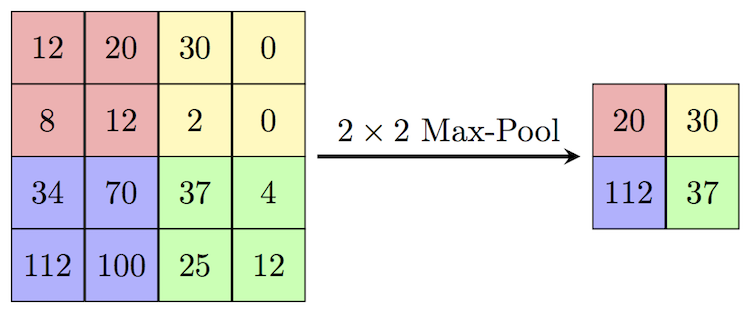
\includegraphics[width=0.6\linewidth]{img/ML/MaxpoolSample2.png}
    \caption{Max pooling operation with kernel size $(2,2)$}
    \label{fig:ML max pool}
\end{figure}

\subsection{Prediction uncertainty and Bayesian models}
In classical supervised deep learning, a neural network with weights $\theta$ is trained on some dataset $\mathcal{D}$ to produce a minimal cost estimator $\hat{\theta}$ for a predefined loss function. From the statistical point of view, this is a point estimate for each one of the network parameter. Point-estimate networks might lack explainability and generalize in overconfident ways to unseen data, and there is no obvious mechanism for such models to express their ignorance in such cases.


This is an analogous situation to classical parameter inference in statistic. From this perspective, the \emph{frequentist} approach to parameter estimation can be compared to point-estimate networks.
However, \emph{Bayesian} statistics \cite{bayesian_stat} has flourished in the last decades and is becoming the dominant statistical framework for data analysis inference problems. In the Bayesian paradigm, parameters are treated as random variables to reflect our ignorance about their ``true'' values. Our prior beliefs about the parameters $\theta$ are then updated in the presence of new data $\mathcal{D}$ using Bayes' theorem:
\begin{equation}\label{eq:Bayes theorem}
    P(H|D) \propto P(D|H)P(H),
\end{equation}
where $H$ is a certain hypothesis about $\theta$, $P(D|H)$ is known as the \emph{likelihood} and encodes the relation between the data generation and the parameters, and $P(H)$ reflect our prior beliefs. Bayesian frameworks have two main advantages. Firstly, they allow us to make our assumptions explicit by setting up the prior $P(H)$. This allows us to clarify, discuss and criticize prior knowledge in a clear way. Secondly, they provide a natural approach to quantify uncertainties in the inference parameters.


Bayesian neural networks are models that incorporate stochastic elements and that are trained using Bayesian inference techniques \cite{BNN_review}. This is generally implemented either by considering stochastic weights in the network, or by considering 
stochastic activations, see \cref{fig:ML BNN ilus}.

\begin{figure}
    \centering
    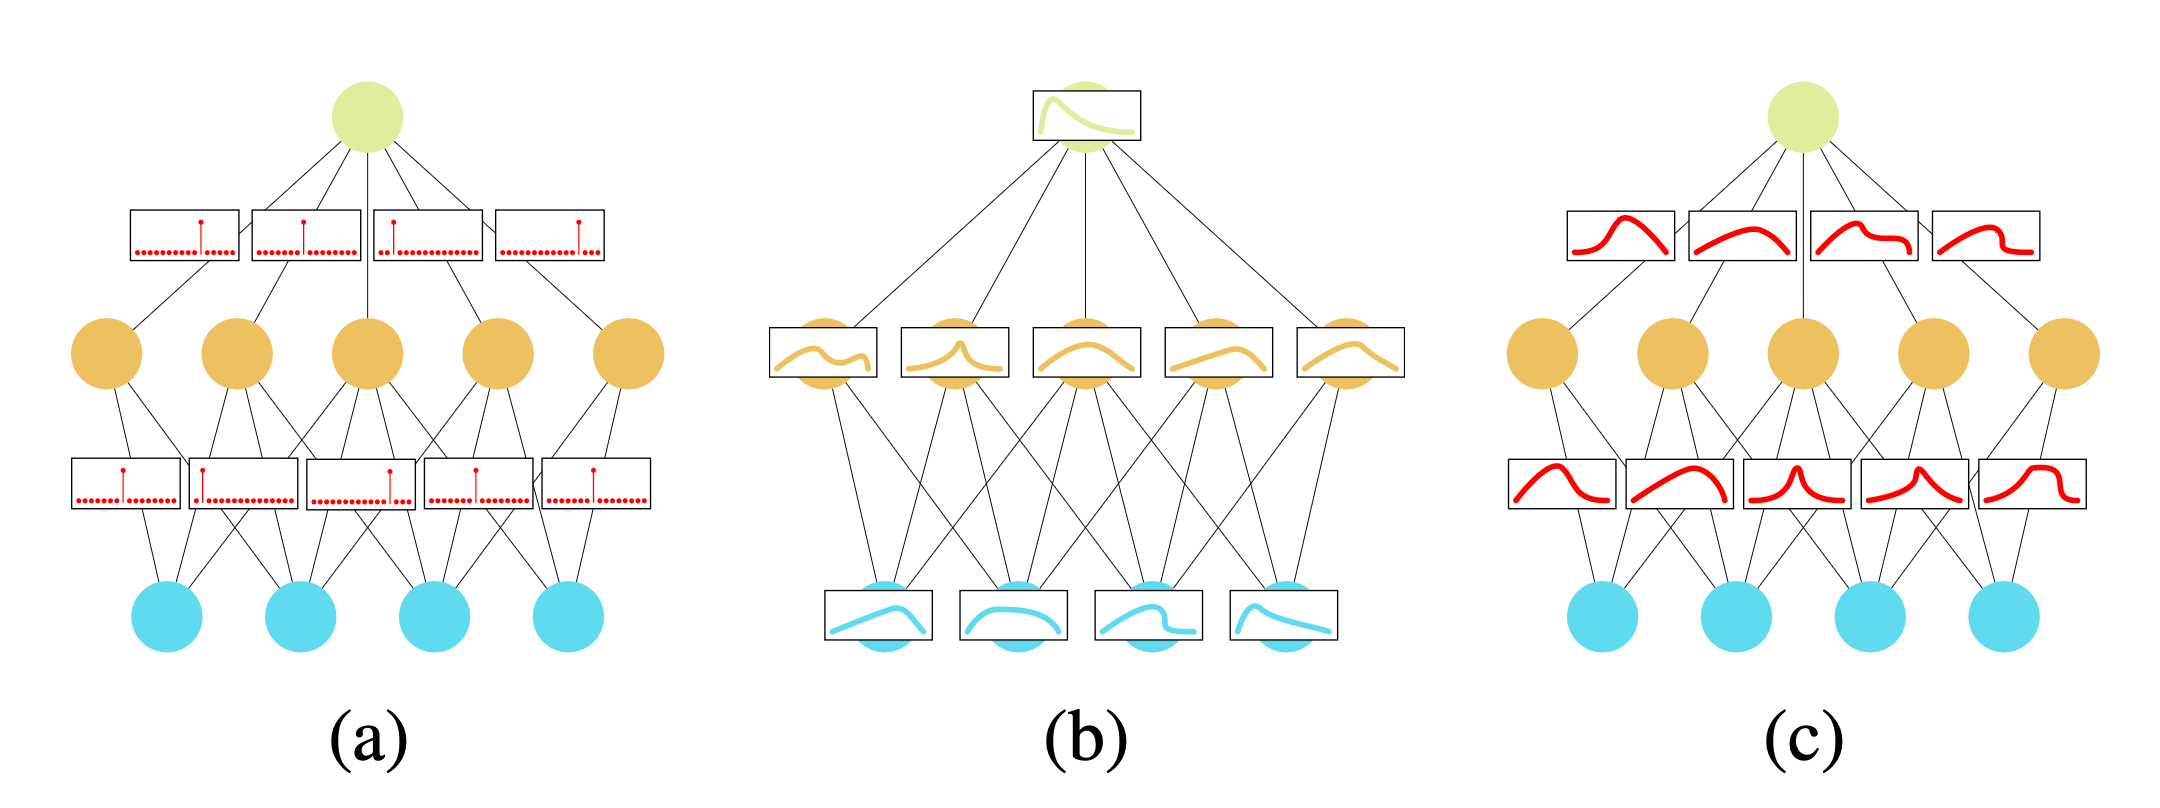
\includegraphics[width=0.9\linewidth]{img/ML/scheme_bnn.png}
    \caption{Illustration for a non-stochastic neural network a), a network with stochastic activations b), and a network with stochastic weights in c). Source: \cite{BNN_review}.}
    \label{fig:ML BNN ilus}
\end{figure}
A Bayesian neural network is defined by a prior distribution over the weights (when they are set to be stochastic), a functional model that forwards the inputs and generates the outputs, and a likelihood model that defines the predictive power of the network $p(y|x,\theta)$. The model weights are update in the presence of data $\mathcal{D}$ according to Bayes' formula
\begin{equation}
    p(\theta|\mathcal{D}) \propto p(\mathcal{D}_y|\mathcal{D}_x, \theta)p(\theta)
\end{equation}
When the model has seen the data, we can use the posterior distribution on the parameters to generate data or make prediction:
\begin{equation}\label{eq:posterior precitive}
    p(y|x,\mathcal{D})=\int_\theta p(y|x,\theta)p(\theta|\mathcal{D}).
\end{equation}
Note that \cref{eq:posterior precitive} weights the predictions by each possible parametrization of the network using the posterior distribution on the weights. In that sense, Bayesian networks can be understood as training an ensemble of networks and then averaging their predictions. Note that ensembles are also a popular technique with classical neural networks \cite{ensemble}. In fact, since the training of a classical network has also stochastic components (the initial weights, shuffling of the data, ...), it is common to train multiple networks with different initialization seeds and weights their predictions, much tend to outperform even the best-performing network.

Let us illustrate how a committee of networks can outperform even a top-performer network. Suppose we train 3 independent networks $A,B,C$ for a classification task with two classes, and that they all have the same error probability $p$. In an exercise of pure democracy \footnote{“I love democracy. I love the Republic”, Senator Palpatine.}, consider a classifier $D$ who picks the class with the majority of votes. Since $D$ is wrong if and only if at most one of the classifiers is wrong, the probability of error for $D$ is (considering $p\to 0$)
$$p^3-3(1-p)^2 =\mathcal{O}(p^2),$$
and hence $D$ outperforms $A,B$ and $C$.


\subsection{Hyperparameter selection}\label{sec:optuna}
The performance and convergence properties of a deep learning model are highly sensitive to its precise architecture, and hence, to the \emph{hyperparameters} that control the latter: number of layers, the exact type of layers (convolutional, dense,...) and other auxiliary parameters that influence the training process. The optimal set of hyperparameters are the ones that produces the best-perfoming model on unseen data. There are three main difficulties when choosing hyperparameters. Firstly, it is not obvious a priori how modifying a certain parameter will affect the performance of a model. For example, if we add an extra layer to a network, will that improve expressivity and performance or will it lead to overfitting? This is a consequence of the low interpretability of deep learning models. Secondly, evaluating the performance of a model requires training it, which is computationally expensive. Finally, there are possibly an infinite number of possible architectures to explore.

Many Python APIs implementing routine to find optimal hyperparameters exists. They include state-of-the-art algorithms for exploring the hyperparameter space, selecting which parameters to explore, and early-stopping the evaluation of unpromising trials. In this work we use \texttt{OPTUNA} \cite{optuna_2019}, which a Python optimization API, to select the appropriate set of hyperparameters for our deep learning models. \texttt{OPTUNA} implements a wide variety of searching algorithms to explore the hyperparameter space. Among those strategies, we can choose a naive grid search, where the user defines a grid over the hyperparameter space, and all possible combination are tested and ranked in a sequential order. \texttt{OPTUNA} can also implement a random search, which randomly selects the next trial over a grid. However, \texttt{OPTUNA} also implements more complex searching algorithms. The default search strategy is the \emph{Tree-structured Parzen Estimator} (TPE) approach. TPE is designed to maximaze the expected improvement when selecting a new sample. If we have already explored a set of points $x$, the expected improvement (EI) for a new trial $y^*$ is defined as
\begin{equation}\label{eq:expected imp}
    \begin{aligned}&\text{EI}_{y^*}(x)=\int_{-\infty}^{y^*}(y^*-y)p(y|x)dy=\int_{-\infty}^{y^*}(y^*-y)p(x|y)\frac{p(y)}{p(x)}dy\end{aligned},
\end{equation}
where we are assuming a one-dimensional problem for clarity, and $p(y|x)$ represents the probability of chossing a trial $y$ having observed $x$, as obtained from the searching algorithm. TPE optimizes \cref{eq:expected imp} by using the following routine \cite{TPE}:
\begin{enumerate}
    \item We initiate a set $\mathcal{D}$ of explored trials with $N_i$ parameters and compute their performance.
    \item $\mathcal{D}$ is split as $\mathcal{D}=\mathcal{D}^l \cup \mathcal{D}^g$ in the top $\gamma$ performers (a common value is $\gamma=0.2$) $\mathcal{D}^l$ and the lower performers $\mathcal{D}^g$.
    \item We fit a two Gaussian mixtured distributions to $\mathcal{D}^l$, l(x) and to $\mathcal{D}^g$, g(x). This is a Kernel Density Estimaton (KDE) for the distribution of both sets. See \cref{fig:ML TPE} for an illustration of this step.
    \item The new trial parameters are selected and added to $\mathcal{D}$ to maximize $l(x)/g(x)$. In practice, this can be done by generating $N_s$ samples from $l(x)$ and then maximizing $l(x)/g(x)$ over those samples.
\end{enumerate}



\begin{figure}
    \centering
    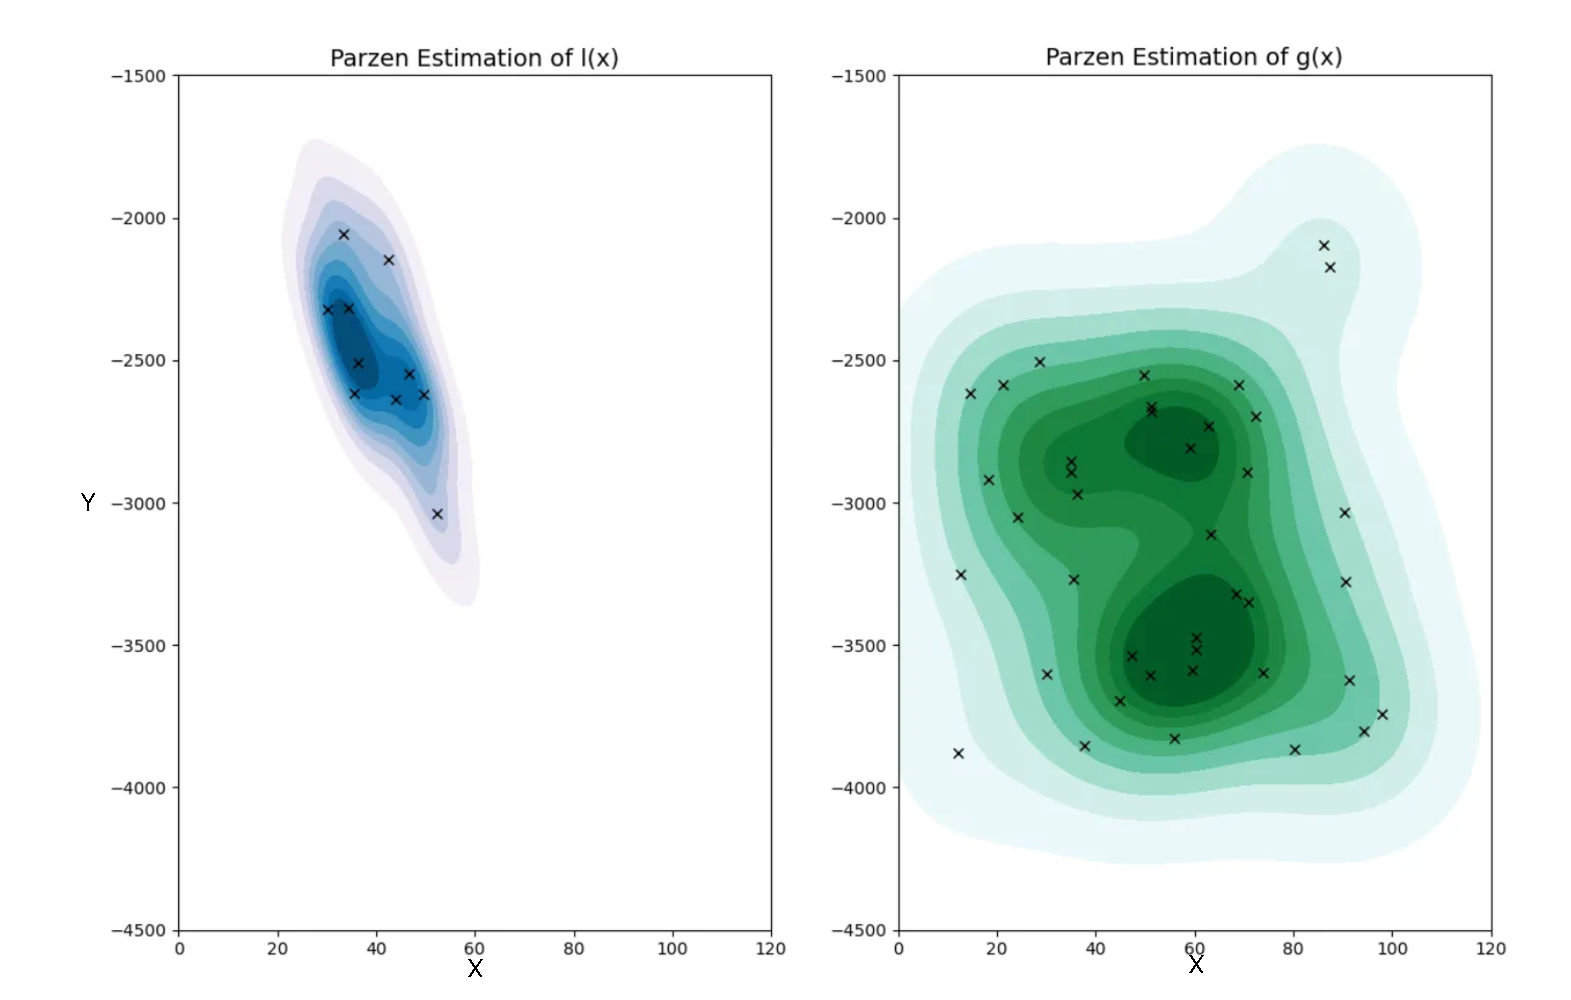
\includegraphics[width=0.6\linewidth]{img/ML/Parzen.pdf}
    \caption{Example DE estimation for the distribution $l(x)$ and $g(x)$ used in the TPE algorithm.}
    \label{fig:ML TPE}
\end{figure}

We can easily show that the TPE routine maximizes the expected improvement \cref{eq:expected imp}.
Firstly, note that $\gamma=p(y<y^*)$ and that $p(x)=\int p(x|y)p(y)dy=\gamma l(x) +(1-\gamma) g(x)$. Furthermore, if $y<y^*$, we have that 
$p(y|x)=l(x)$, and hence,

\begin{equation}
    \int_{-\infty}^{y^*}(y^*-y)p(x|y)p(y)dy=\ell(x)\int_{-\infty}^{y^*}(y^*-y)p(y)dy=\gamma y^*\ell(x)-\ell(x)\int_{-\infty}^{y^*}p(y)dy.
\end{equation}
We conclude that 
\begin{equation}
    \text{EI}_{y^*}(x)\propto \left(\gamma+\frac{g(x)}{\ell(x)}(1-\gamma)\right)^{-1},
\end{equation}
and so we need to maximize $l(x)/g(x)$, as previously discussed.




\subsection{Loss function and training}
In this section, we further detail to training process of a deep learning model, and describe the alhorithms that will be used to train our model.
As we have already discussed in section \ref{sec: dataset}, the goal of our model is the minimize the generalization error:

\begin{equation}
    \varepsilon =\mathbb{E}_F[\mathcal{L}(Y,\hat{f}(X|\mathcal{D}_T))].
\end{equation}
The loss function $\mathcal{L}$ should be choosen to encourage the model to produce realisitc outputs. For regression, where the goal is to estimate an output tensor $Y$ from an input $X$, typical choices include the usual Euclidean norm or the absolute difference:

\begin{equation}\label{eq:euclidean norm}
    \mathcal{L}(Y,\hat{Y})=\sum_i |\hat{Y}_i-Y_i|^p, p=1,2,
\end{equation}
where $\hat{Y}$ is the model prediction. This choise of loss function is minimzed when the model correctly predicts the target tensor.
An important information to note is that \cref{eq_ch3:global_loss} is generally unkown, since we don't have acces to all the possible realizations of the data, but only to a limited training dataset. As a consequence, we typically minimize the loss function computed on small samples of the training data, called \emph{batches}, by averaging the loss over all samples in the batch. Observe that then, computing the average loss over a large batch will yield a closer approximation to the true loss function. The training process then uses these estimations of the loss to update the network parameters, $\theta$, using techniques that involve the computation of the loss gradient. This process is normallh repeated multiple times over the training dataset. Each time the model sees the whole dataset is knwown as an \emph{epoch}. A training loop with $N_e$ epochs and batches of size $B_s$, with $N_b$ batches, can then be written as:

\begin{algorithm}
    \caption{Classical deep learning training loop}\label{alg:training loop}
    \begin{algorithmic}
    \While{$\text{epoch} <N_e $}
        \While{$\text{batch} <N_b $}
        \State $\text{Loss}\gets \frac{1}{B_s}\sum_i\mathcal{L}(\hat{Y_i},Y) $
        \State Compute $\nabla_\theta (\text{Loss})$
        \State Update $\theta \gets \theta(\nabla_\theta (\text{Loss}))$
        \EndWhile    
    \EndWhile
    \end{algorithmic}
    \end{algorithm}

In algorithm \ref{alg:training loop} there are two main steps we have not specified. Firstly, the comoutation of $\nabla_\theta (\text{Loss})$. This is trivial from the mathematical viewpoint, but it is not trivial to implement\footnote{Note that this is purely a computer science problem.}. Most APIs implement a \emph{backpropagation} algorithm for this step that we will not discuss here\footnote{\url{https://www.tensorflow.org/guide/autodiff}}. The second key aspect of a training loop is using the gradient $\nabla_\theta (\text{Loss})$ to update $\theta$. This step in algorithm \ref{alg:training loop} was repreented by $\theta \gets \theta(\nabla_\theta (\text{Loss}))$. The precise way of using the calcualted loss gradients to update the weights define the \emph{optimizer}\footnote{Note that this is purely a mathematical problem in optimization.}. A naive way to optize the loss at each iteration is to use the most straightforward implementation of \emph{gradient descent}, where the parameters are updated using
\begin{equation}
    \theta \gets \theta - \alpha \nabla_\theta (\mathcal{L}),
\end{equation}
where $\alpha$ is a constant known as the \emph{learning rate}. In general, optimizing the loss function $\mathcal{L}$ corresponds to optimizing a complex (perhaps non-convex) function on a highly multidimensional space, with millions or billions of parameters. As a consequence, naive gradient descent might not be the best-performing optimizer. Additionally, recall the loss $\mathcal{L}$ calculated for every batch is just an approximation of the global loss \ref{eq_ch3:global_loss}. The batch size determines how accurate the computed gradient is. Calculating the loss over all possilbe data points would yield the exact gradient. On the opposite extreme, calculating the gradient on a single data point would generate a biased gradient, and lead to a noisy gradient descent. The loss function can also have a complex strucuture. In the literature, a multitude of optimizers that improve and generlize the naive gradient descent exist. In this work, we use \emph{Adam} \cite{adam}. Adam is a first-order momemtum-based optimizer. Adam uses recursive update of the first and second moment of the gradient to update the learnable parameters. The Adam algorithm reads as follows:

\begin{algorithm}
    \caption{Adam optimizer}\label{alg:adam}
    \begin{algorithmic}
            \Require $\alpha$ : Learning rate
            \Require $\beta_1, \beta_2$: Moment decay rates
            \Require $f(\theta)$: Target function
            \Require $\theta_0$: Initial parameters
            \Require $\varepsilon$: Numerical tolerance constant
            \State $m_0 \gets 0$: Initialize first moment
            \State $v_0 \gets 0$: Initialize second moment
            \State $t \gets 0$: Initialize time
            \While{$\theta_t$ not converged}
                \State $t \gets t+1$
                \State $g_t \gets \nabla_\theta f(\theta_{t_1})$: Get gradient
                \State $m_t \gets \beta_1 m_{t-1}+(1-\beta_1)g_t$: Update first moment
                \State $v_t \gets \beta_2 v_{t-1}+(1-\beta_2)g_t^2$: Update second moment
                \State $m_t \gets m_t/(1-\beta_1^t)$: Correct first moment bias
                \State $v_t \gets v_t/(1-\beta_2^t)$: Correct second moment bias
                \State $\theta_t \gets \theta_{t-1}-\alpha m_t/(\sqrt{v_t}+\varepsilon)$: Update parameters
            \EndWhile


    \end{algorithmic}
\end{algorithm}
Adam differs in two key features with respect to the naive gradient descent. Firstly, it includes two decay constants $\beta_1$ and $\beta_2$ used to include information about the past state of the optimization into the next current step. Since typical values are $\beta \sim 0.9$, recent gradient values contribute more to the current step update than older ones, but the inclusion of a momentum term allows the optimization to potentially escape local minima. Secondly, Adam includes a term $v_t$ to account for the second moment in the gradient estimation. The running averages in Adam can potentially help to navigate noise functions by smoothing the local gradient.


Most current deep learning implementations are deployed or trained using HPC infrastructure. This becomes a necessity when training on large datasets. A quickly deployable way of paralellize training, and which requires minimal code modification is known as \emph{Synchronous Distributed Training}. Synchronous Distributed Learning aims to harvest to computational power of multiple machines (GPUs,...) in the training stage by having different workers perform parallel calculations in a single batch. This can be done, for instance, by splitting the batch and sending each part to a different worker. In this work, we use the TensorFlow implementation \texttt{tf.distribute.MirroredStrategy}. This training strategy mirros the model and its parameters in every worker (for instance, in every GPUs), slices the training batch and distributes them accross all workers. Each worker then calculates the loss and gradient in the corresponding batch slices. The gradient is then aggregating before updating the parameters and moving onto the next batch.

\begin{figure}
    \centering
    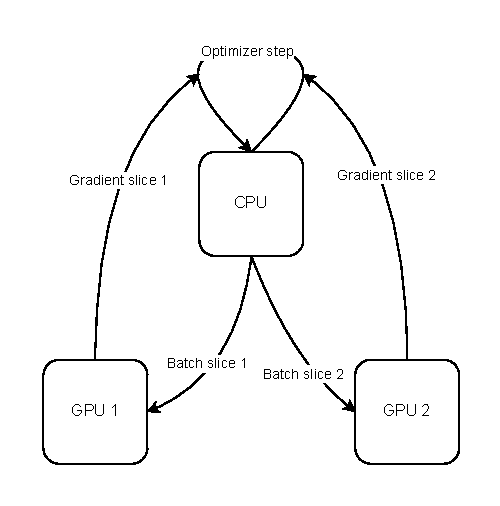
\includegraphics[width=0.6\linewidth]{img/ML/mirror_training.drawio.pdf}
    \caption{Distributed mirrored learning strategy with two workers (GPUs) and a CPU agregating the gradient and updating the model parameters.}
    \label{fig:ML mirror training}
\end{figure}

\section{Workflow implementation: Recovering IGM conditions from the Lyman-alpha forest }
This section describes the deep learning implementation used in this work and built in the ideas that have already been introduced regarding machine learning. The code used is largely based on \cite{nasir2024deep} with very minor modifications and is avaible at \url{https://github.com/nicenustian/bh2igm} and based on TensorFlow and TensorFlow Probability.


The ultimate aim is to use a Bayesian neural network to recover the IGM gas density from an input Lyman-$\alpha$ skewer. Note that this is essentially equivalent to invert Equation \ref{eq:lyman opacity}, which describes the Lyman-$\alpha$ opcaity as a function of the IGM gas conditions. As we have already discussed int \ref{sec: optical depth weighted}, we will work int the optical depth-weighted space. This avoids two main potential difficulties in the anaylisis. Firstly, by working in this new space, the network will not have to learn the relation between peculiar velocities and the Lyman-$\alpha$ opcaity, which simplifies both the architecture design and learning phase. Secondly, it breaks the degeneracy introduced by peculiar velocities, since a shift in the physical space can produce the same opacity as a shift in the velocity space.

We specify the architecure design by the hyper-parameter list found in \cref{table: fiducial architecture}. The global architecure that describe the number and size of the layers is specified by two hyper-parameters. Firstly, the parameter ''Layers per block'' is an integer list whose size is the number of blocks in the network and whose elements are the number of layers in each block. Secondly, the parameter ''Filters per block'' is also an integer list that specifies the number of convolutional filters of the layers for each block. If the architecure is a simple MLP, this parameter does not have any affect. The layers are choosen among a simple densly connected layer (MLP), and convolutional layer (ConvNet) or a residual layer (ResNet). Every feedforward pass through a convolutional or densely connected layer is followed by a batch normalization layer and by an activation function, see section \ref{sec:deep learning archi}. We use the PReLU activation function, wich is a generalization of the ReLU activation with a learnable weight $\alpha$ such that:
\begin{equation}
    \text{PReLU}(x;\alpha)=
    \begin{dcases}
        \alpha x &  , x<0\\
        x & , x\geq 0
    \end{dcases}
\end{equation}
We append the same final block to all three potential architecutres, which consists of a flattening layer transforming the tensor being manipulated to a one-dimensional vector, a dense layer a finally a Gaussian probabilistic layer.
This final block includes the stochastic components of the neural network (hence the name Bayesian). For each target output density pixel the Gaussian layer outsputs a full Gaussian probability distribution parametrized by the expected density and the standar deviation. This standar deviation will later be used as the estimation for the espistemic uncertainty in the network prediction. We illustrate the fiducial architecture in \cref{fig:ML nn architecture}.
\begin{figure}
    \centering
    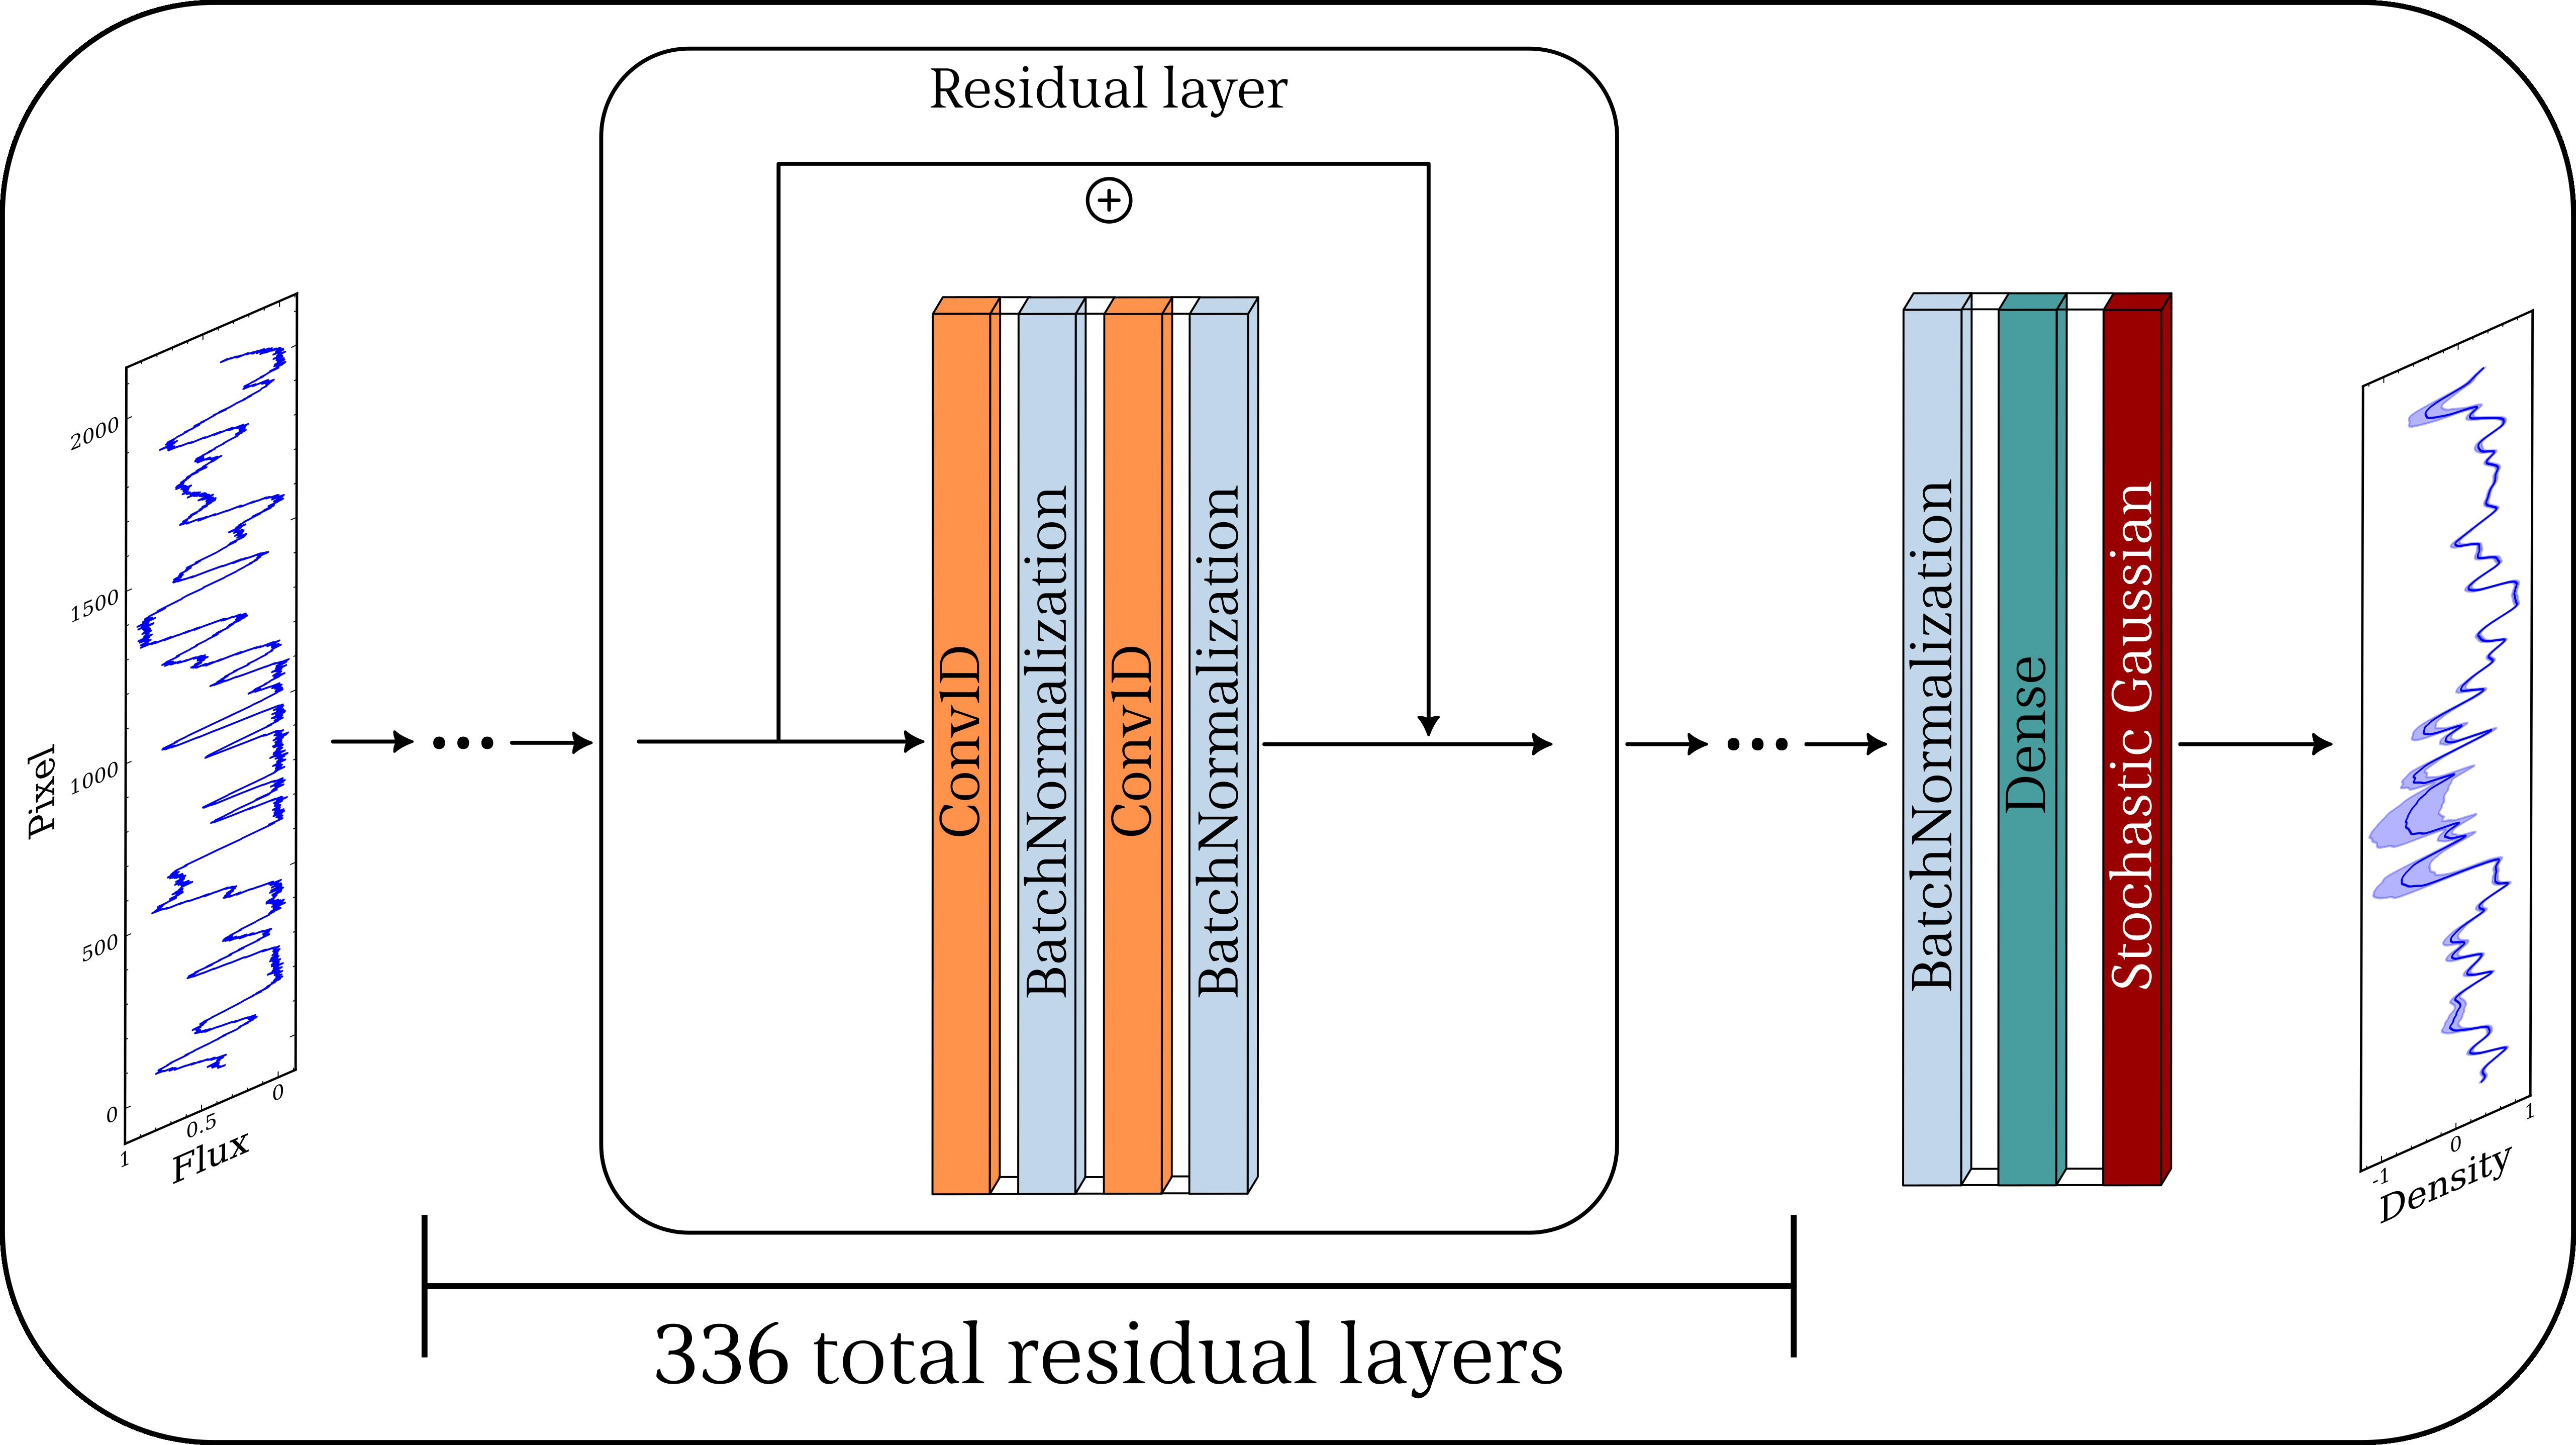
\includegraphics[width=1\linewidth]{img/ML/nn_archi.jpg}
    \caption{Fiducial architecture for our Bayesian neural network trained at $z=4.4$ on the Sherwodd simulation suite. The fiducial parameters can be found in \cref{table: fiducial architecture}.}
    \label{fig:ML nn architecture}
\end{figure}

We optimize the netowork hyper-parameters using \texttt{OPTUNA} as discussed in section \ref{sec:optuna}. Table \ref{table: fiducial architecture} the optimized hyper-parameters and the range considered during the grid search. Note that these values can potentially deppend on the nature of the training dataset, and hence may vary with redshift. In table \ref{table: fiducial architecture} we present the fiducial architecture at $z=4.4$. This optimizating process is automatically carried out whenever the redshift is varied.

For each redshift, we train a different network using the Sherwood simulation suite presented in section \ref{chap:sherwood}. Recall that we consider two training datasets, \texttt{SHERWOOD} and \texttt{SHERWOOD THERMAL}, where the latter includes variations in the thermal parameters and reionization history. See \cite{sherwood_wdm} for more details. The inclusion of thermal parameters will lead to a more robust network when used on unseen real data, but its performance will naturally be lower than the network trained on a single thermal hsitory. We use \texttt{SHERWOOD} for an initial model testing, and \texttt{SHERWOOD THERMAL} for our final anaylisis on real data. 80 \% of the data is used for training, and the rest is used for validation purposes. For reference, the training dataset \texttt{SHERWOOD} with,7 different WDM models has a total size of $\sim 3.5$ GB. We use the Raven\footnote{\url{https://www.mpcdf.mpg.de/services/supercomputing/raven}} HPC cluster at the Max Planck Computing and Data Facility to train our networks. With 4 Nvidia A100 GPUs, a typical training time is $\sim 1$ hour, depending on the model's exact architecture and number of parameters.


\begin{table}
    \centering
    \begin{tabular}{|c|c|c|c|}
        \hline
        Hyper-parameter&Min.  &Max.  &Best value \\
        \hline
        Layers per block (int)& 1 & 4 & [1, 2, 4 ,4] \\
        $\log_2$(Filters per block) (int)&$1$  &$5$  &  [4, 5, 5, 5] \\
        Number of blocks (int)&1  &4  &4 \\
        $\log_2$(Batch size) (int)&3  &8  & 3 \\
        Learning rate ($\log_s$, float)&$10^{-4}$  & $0.1$  &0.004937 \\ \hline
        Network (MLP, ConvNet, ResNet)&...  & ... &ResNet \\
        \hline
    \end{tabular}
    \caption{Hyper-parameter grid search for the fiducial model at $z=4.4$. ``$\log_s$'' indicates the parameter is sampled in the log domain. ``Int'' and ``float'' mean they are sampled as integers or floats, respectively.}
    \label{table: fiducial architecture}
\end{table}


The network's input consist of a Lyman-$\alpha$ flux skewer, and the network's output consists of the mean density and standard deviation at each pixel. The labelled training data consists of individual Lyman-$\alpha$ flux skewers with their associated density optical depth-weighted density field, $(F,\log(\Delta_\tau))$. For each labelled training pair, the loss function is taken to be the negative log-likelihood (NLL) for the normal distribution that the network parametrizes:

\begin{equation}\label{eq:our loss}
    -\log\mathcal{L}=\frac{1}{N}\sum_{{\mathrm{i}}}\left((Y_{{\mathrm{i}}}-Y_{{\mathrm{i},\mathrm{pred}.}})^{2}/\sigma_{{\mathrm{i},\mathrm{pred}.}}^{2}+\log(\frac{1}{\sigma_{{\mathrm{i},\mathrm{pred}.}}^{2}})\right),
\end{equation}
where the sum runs over all skewer pixels,$Y_i$ is the real density at pixel $i$, $Y_{{\mathrm{i},\mathrm{pred}.}}$ is the predicted expected density and $\sigma_{{\mathrm{i},\mathrm{pred}.}}^{2}$ the predicted standard deviation.

The input skewers are processed as follows. Firstly, the input flux is rebinned into a target number of pixels to match the real data that will be used. Downsampling is done by taking the avarage flux over nearby pixels, while upsampling is done by appending to every pixel a copy of itself. The flux is then convolved using a gaussian kernel to simulate a given instrumental resolution. In most of our analysis the resilution is taken to be $6$ km/s, in accordance with state-of-the-art spectrographs, such as UVES \cite{UVES}. During training, the training data is stacked and randomly shuffled to ensure a correct mixing and representativity of the models. Lastly, we process the reescale input optical depth to match the observed mean flux at the considered redshift \cite{Becker_mean_flux}.
The training data is augmented on-the-fly in two ways. We first roll the input spectra by application translations, this helps the network learning dynamical features, independently of their positions. We also add random uncorrelated gaussian noise to simulate a finate signal-to-noise ratio (SNR). The default SNR per pixel used for testing purpises is 50. When applying our methods to real-data, the network is retrained using a noise model for each target object.


We use the Adam optimizer with fixed moment decay rates as implementation in the TensorFlow API and a learning rate set by the Optuna grid search. The training is evaluated using two main metrics: the loss function NLL, and the mean absolute error, MAE, defined as the Euclidean norm \ref{eq:euclidean norm} in with $p=1$. To prevent over-fitting, the network parameters are only updated if the NLL loss improves on the validation split of the data. A policy to halve to learning rate if there is no loss improvement in the test set for 10 epochs is also included. This is the most straightforward adaptation of an adaptive learning rate. Figure \ref{fig:ML learning curve} shows the evolution of the NLL and the MAE on the validation split during training for our fiducial architecture at $z=4.4$ and the \texttt{SHERWOOD} suite. It is interesting to note that while the MAE is always positive by definition, negative valueso of the NLL are consistent with its definition. Figure \ref{fig:ML learning curve} demostrates that, for our problem, the network training coverges in $\sim 100-150$ epochs. Recall that we always work with $\log(\Delta_\tau)$, which also serves as a regulatization step with respecto to the density.


\begin{figure}
    \centering
    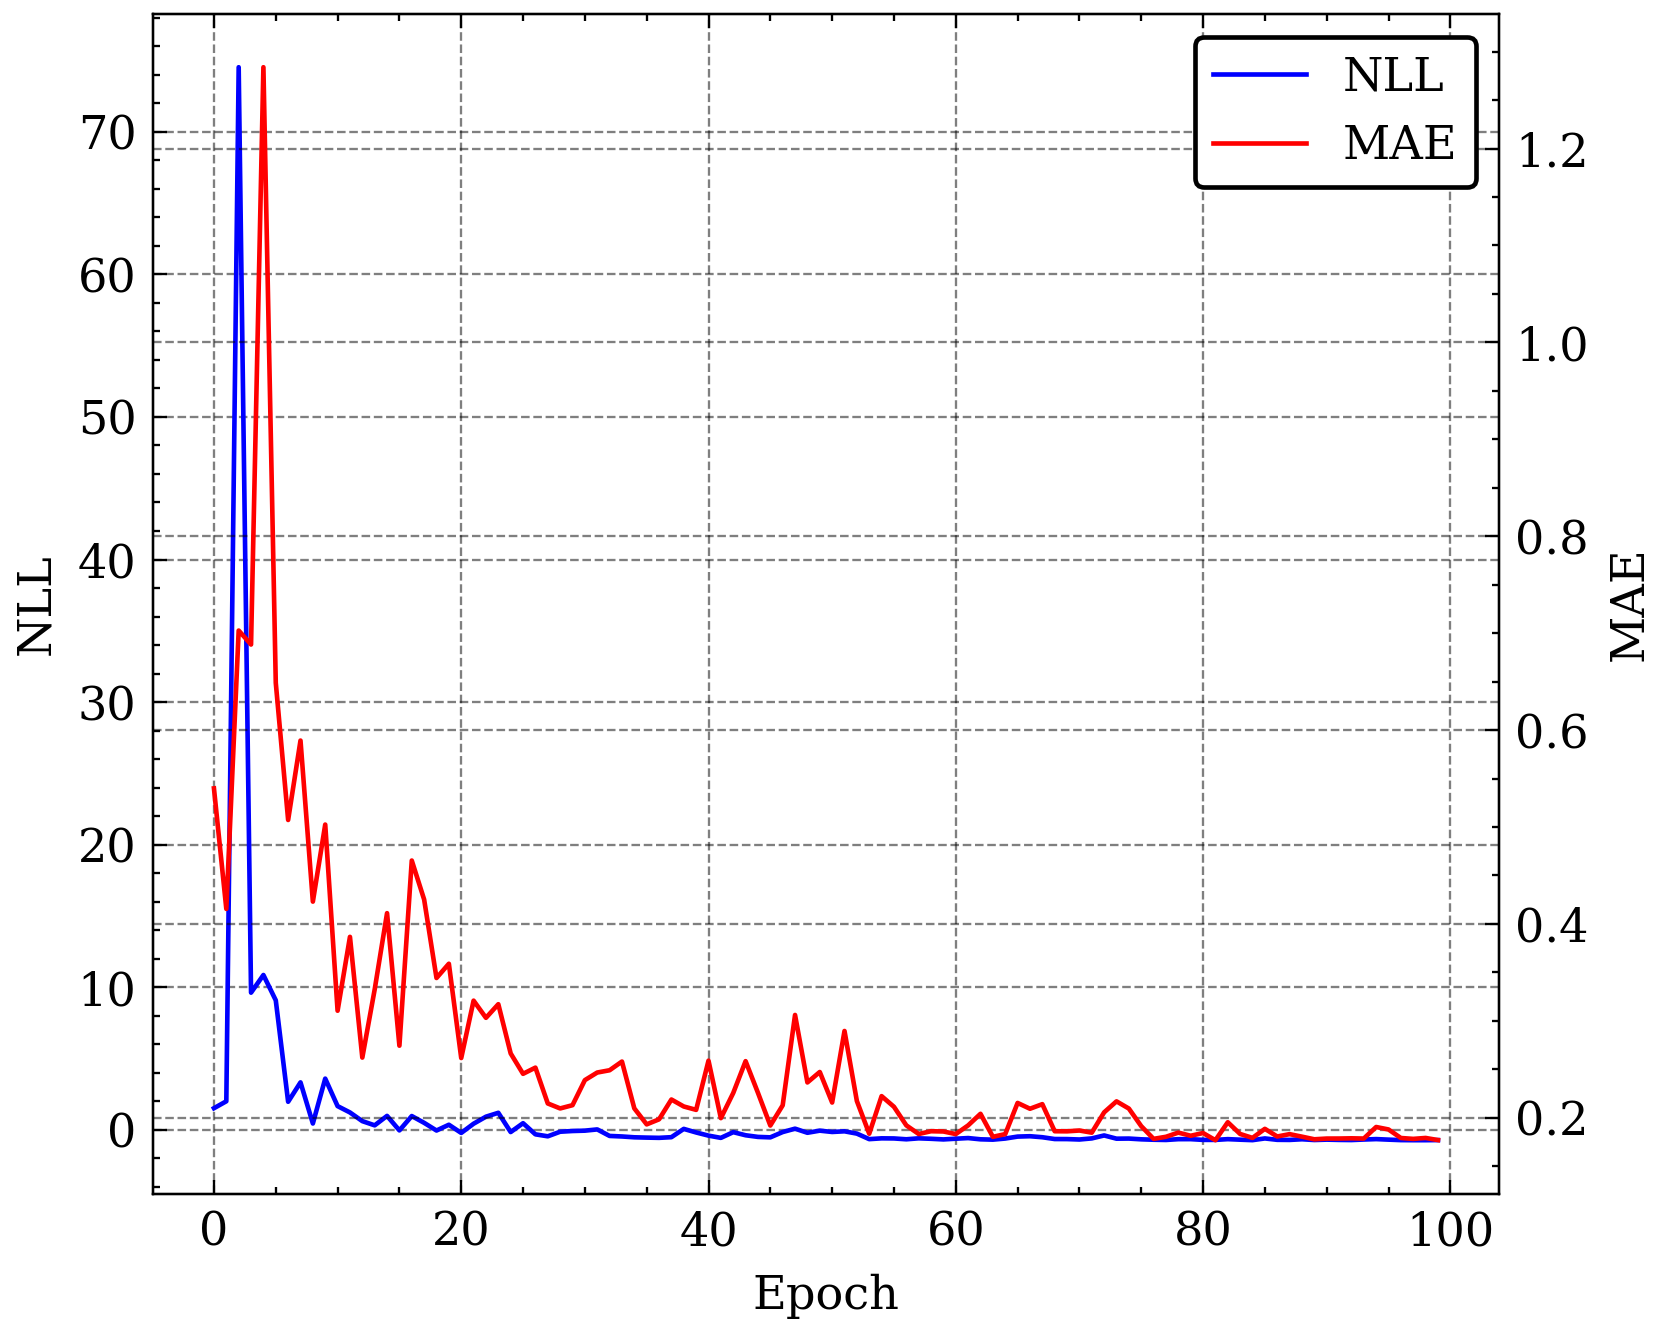
\includegraphics[width=0.7\linewidth]{img/ML/learning_curve.png}
    \caption{Learning curve for our fiducial architecture at $z=4.4$ on the \texttt{SHERWOOD} dataset. The figure shows the NLL and the MAE on the validation split as a function of the epoch.}
    \label{fig:ML learning curve}
\end{figure}

In \cref{fig: example_recovered_skewer} we show an example 20h$^{-1}$cMpc  Lyman-$\alpha$ validation skewer from the \texttt{SHERWOOD} dataset. The top panel shows the input flux to the network. The bottom panel shows the true $\Delta_\tau$ density fields, the (mean) recovered densities and the $1\sigma$ envelope predicted by the Bayesian network. Note that, in the spectral regions with large features and variations in the flux, the predicted mean density closely follows the true field. In those regions, there is enough physical information for the network to accurately recover $\Delta_\tau$. In contrast, in the saturated regions with low flux, the noise dominates, and the network predicts larger uncertainties (observe, for instance, the saturated region in Figure \ref{fig: example_recovered_skewer} around 8h$^{-1}$cMpc). This should be regarded as a strength of Bayesian netoworks, since they are able to accurately detect and make explicit situations where the predictions should not be trusted. To minimize the mean error in regions where the network cannot make accurate preditions, note how there is a bias towards quasi-constant mean prediction. This is visible around 8h$^{-1}$cMpc, where the true density has a steep increasing profile, and the predition has an almost constant u-shaped profile.

\begin{figure}
    \centering
    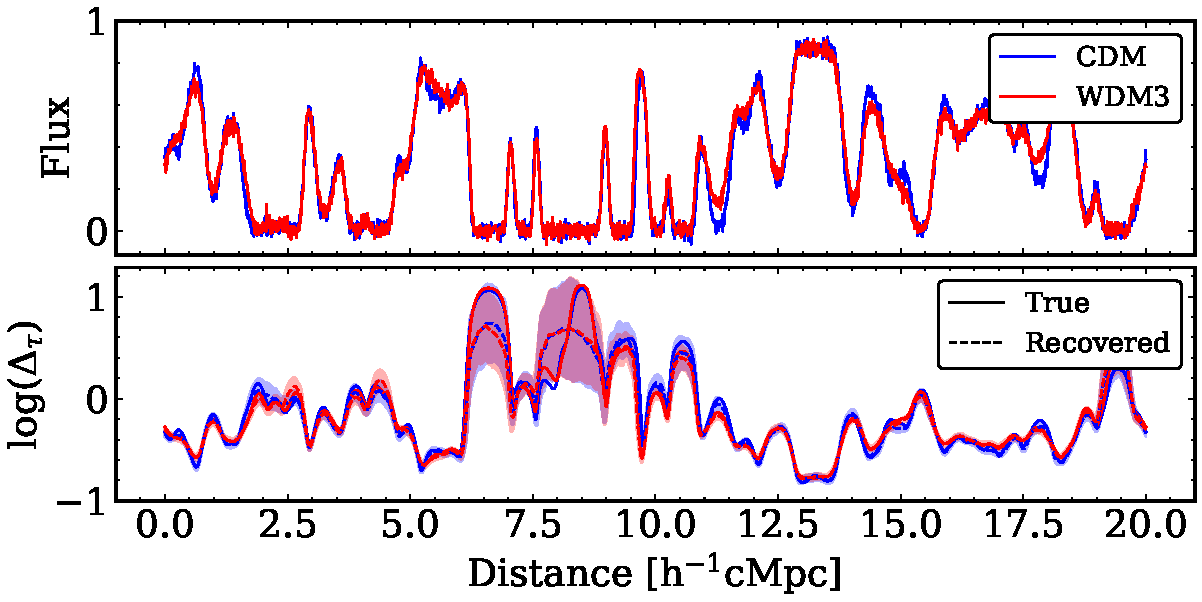
\includegraphics[width=0.99\linewidth]{img/ML/skewer.pdf}
    \caption{An example 20h$^{-1}$cMpc Lyman-$\alpha$ validation skewer for the CDM and WDM3 Sherwood models. The top panel shows the input flux to the network. The bottom panel shows the true $\Delta_\tau$ density fields, the (mean) recovered densities and the $1\sigma$ envelope predicted by the Bayesian network.}
    \label{fig: example_recovered_skewer}
\end{figure}
On the \texttt{SHERWOOD} validation split, the network reaches a $1\sigma$ accuracy of $79\%$, meaning that $79\%$ of the pixels are correctly predicted within $1\sigma$. Note that this is a larger accuracy that expected from purely normally-distributed densities.




 ,.... violin...compare thermal models and non thermal










\section{Recovered field statistics and uncertainties}\label{sec:recovered statistics}
Once we have a machinery to recover the IGM density from a Lyman-$\alpha$ skewer, we would like to use this density field information to do statistical inference on the physical parameters of interest. In this work, since the WDM mass directly affects the matter distribution of the Universe (see Figure \ref{fig:villasenor_wdm}) we would like to infer the WDM masses from the recovered $\Delta_\tau$ field. Now, note that the exact $\Delta_\tau$ field of a skewer, such as the one shown in Figure \ref{fig: example_recovered_skewer}, not only depends on a set of physical paramters (WDM mass, temperat,...) but also on the initial conditions or equivalently, the random seed in the cause of a simulation. As a consequence, we will not compare densities on a sightline by sightline basis, but rather compute and comapre agregatted statistics of the fields over multiple realizations that capture global statistical properties, and not simulation-specific characteristics. Statistics that have been amply tested in the literature are the Power Spectrum (PS), the Probability Distribution Function (PDF), the curvature, or the autocorrelation function (see
\cite{Gaikwad_2021} and \cite{wolfson2023forecastingconstraintshighzigm} for more details). In this work we will focus on the $\Delta_\tau$ PDF. In section \ref{sec:IMNN} we will address the optimiality of this choice. 

ADD bootstrapping and PDF OF PDF
ADD MATRIX CORR and resampling and recoveries using finite skerwers

\begin{equation}\label{eq: residuals}
    r_i=\frac{\Delta_{\tau,i}-\mu_i}{\sigma_i}
\end{equation}



PDF:
\begin{equation}\label{eq:PDF of PDF}
    p(\lambda |f(x),N )\propto \frac{\Gamma(N+1)}{\Gamma(N\lambda+1)\Gamma(N-N\lambda+1)} f(x)^{N\lambda}(1-f(x))^{N(1-\lambda)}
\end{equation}



\section{Model interpretability}
Deep learning models tend to have, by definition, numerous parameters. As a consequence, giving an interpretation for individual model parameters is far from being a trivial task. On top of the large number of parameters, the nonlinearities and the potentially biased and uncomplete dataset can lead to complex training behaviors. In that regard, deep learning models have classically been regarded as ``black-box'' models. They are often more accurate than simpler statistical models, but lack explainability. Great efforts have been recently made in undertanding the learning dynamics of neural networks \cite{shwartzziv2017opening}, \cite{buhrmester2019analysis}.
Due to the complexity of this interpretation task, here we choose to only give a qualitative analysis of some aspects that can help gain intuition on how the newtork operate internally.

Although many open-source libraries, such as \textit{Captum}\footnote{https://github.com/pytorch/captum}, implement popular methods for deep learning model visualization and interpretation, in this work we use TensorFlow's built-in'differentiation capabilities. In particular, we use Automatic Differentiation to compute the \textit{saliency} score of the model, defined as the gradient of the model output with respecto to the model input. As a consequence, for every target density pixel, the saliency score measure which flux pixel variation contributes the most to a change in density. Saliency is a simple socre giving us insights into how the model uses flux to recunstruct densities. Additionally, note that calculating such gradients do not requeire any numerical finite diffrence approximation, since TensorFlow's GradientTape class can build an exact computational graph with all the operations performed on the input flux. The saliency at density pixel $i$ and input flux pixel $j$ is simply

\begin{equation}
    \text{Saliency}(i) = \frac{\partial  \mu_i}{\partial f_j}.
\end{equation}

Figure \ref{fig: saliency} shows the saliency profile averaged over all output density pixels. This gives a global average metric on the relevant flux pixels to predict the density at a certain pixel. The typical saliency ``length'', that is, the typical number of pixels from the pixel center that are useful to predict its density is $\sim 30$. Since at redshift $z=4.4$ our pixel scale on the \texttt{SHERWOOD} data is $1.3$ km/s, we obtain that in velocity space a window of $\sim 40$ km/s is needed to recover the density at a pixel. This particular dynamic is coherent with the underlying physical process, which is a strong robustness sign of our machine learning model. In fact, for the typical IGM gas in the \texttt{SHERWOOD} suite, the Lyman-$\alpha$ absorbtion cross-section profile has a typical scatter of (see Equation \ref{eq:lyman opacity} $ b(T) \sim 20$ km/s.


\begin{figure}
    \centering
    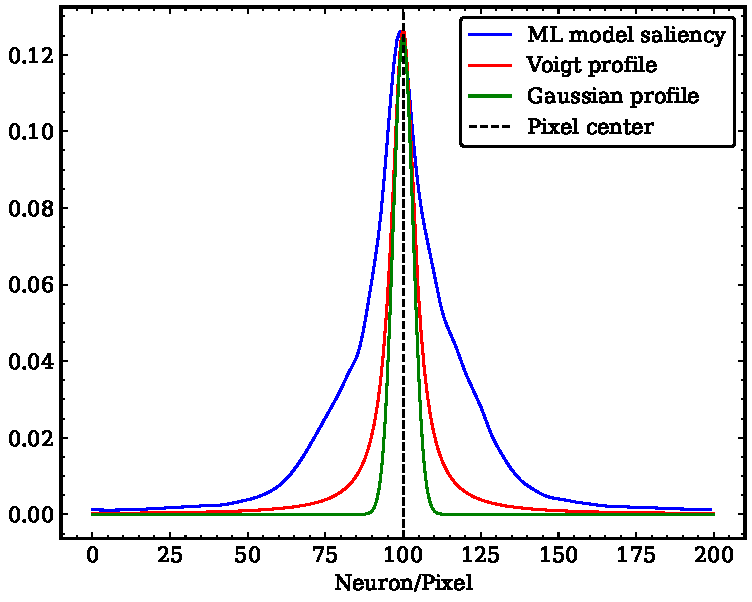
\includegraphics[width=0.6\linewidth]{img/ML/saliency.pdf}
    \caption{Saliency of the CDM and WDM3 Sherwood network at 8h$^{-1}$cMpc Lyman-$\alpha$ flux.}
    \label{fig: saliency}
\end{figure}



As we have already mentioned when discussing Figure \ref{fig: example_recovered_skewer}, saturated regions lead to larger uncertainties in the network's predictions, reflecting the fact that noise dominates over the physical signal. Observe again the saturated region around 7h$^{-1}$cMp and 8h$^{-1}$cMp in Figure \ref{fig: example_recovered_skewer}. Both of these regions have completly different density profiles, but the network predicts the same u-shape profile with a similar peak density. This peak density is slighlt above the mean density in the simulation box and is similar for the CDM and WDM3 models. We can interpret this as the network leaning a unique mean ``high-density'' value for saturated regions and the whole dataset.



talk about the no train tests
weird inputs
filters number, values, activation.
saliency








\chapter{Constraining Warm Dark Matter at the density level}\label{sec: inference pipeline}


\section{Inference pipeline: from Lyman-alpha skewers to WDM constraints}\label{sec: inference algo}

In section \ref{chap: deep learning} we have given a detailed analysis of our Bayesian deep-learning algorithm to recover IGM densties from a Lyman-$\alpha$ skewer. The baryonic density of the IGM is sensitive to the WDM mass through a clear physical mechanism related to gravitational clustering. In this section, we use the recovered IGM density fields to constrain WDM candidates. Note that the natural observable quantity related to the Lyman-$\alpha$ forest is the flux. As a consequence, an almost omnipresent choice in the literature has been to work directly with summary quantities on the flux, which is a proxy of the underlying density. Such summaries include the power spectrum (PS) \cite{Villasenor_2023}, the curvature \cite{Becker_2010}, the probability distribution function (PDF), etc. The deep-learning approach introduced in section \ref{chap: deep learning} allows us to directly recover the baryonic density field along a line of sight, thus having full acces to the field level IGM properties. In this section, we use the recovered $\Delta_\tau$ fields by our neureal network to constraint WDM directly at the density field level. Recall Figure \ref{fig:villasenor_wdm} and Figure \ref{fig: exact density PDF} showing how different WDM models affect the density field. We strive to capture that difference in the WDM models to constrain which free-streaming length are compatible with QSO observations. Note that for a given line of sight, the precise value of the density field not only depends on the WDM masses ( and other possible physical paramters), but most crucially it depends on the random density fluctuation that have seeded the gravitational collapse process. Equivalently, in a simulation setting, the obtained densities would depend on the seed used to initiliaze each simulation. This makes infeasible to campare a given Lyman-$\alpha$ skewer to a simulated one, and means that we must use aggregated summaries over multiple skewer that capture the global properties of the field. In this work, we perform the inference use the density PDF as the summary statistic of choice. This is a well-tested and robuat statistic \cite{Gaikwad_2021}. In section \ref{sec:IMNN} we give an additional argument, based on Information Maximising Neural Networks, to support this choice of summary statistic.


The basic working principle of inference pipeline is to fit the observed $\Delta_\tau$ PDF, with its associated uncertainties, to the corresponding $\Delta_\tau$ PDF produced by each WDM model. To compare similar quantities, we always work with the recovered field by our neural network from section \ref{chap: deep learning}. Note that in the \texttt{SHERWOOD} only a finite number of DM models are avaible, due to the computational cost of running this simulation. In more detail, we only have acces to the models CDM, and WDM1,2,3,4,8,12. We smoothly and linaerly interpolate the PDF by interpolating each PDF bin to generate a $\Delta_\tau$ PDF in the range of WDM masses from 0 to 1 KeV. Note that, since we expect the real observations to fall close to the CDM model, and have multiple simulations close to CDM, we expect this interpolation not to limit the inference pipeline. See Figure \ref{fig: exact density PDF} again and observe how similar are the PDF for CDM and WDM3. For more massive models in $\texttt{SHERWOOD}$ the PDF converge to the CDM PDF.

For each DM model of inverse mass $m$ we denote by PDF($m$)  the $\Delta_\tau$ PDF computed over the recovered densities by our NN network over all avaible sightlines in the \texttt{SHERWOOD} or \texttt{SHERWOOD THERMAL} datasets. We refer to this as the model PDF. Let us denote by $\widehat{\text{PDF}}$ the recovered PDF for a target set of (observed) skewers. Then, we fit $\hat{\text{PDF}}$ to the model PDFs using a simple $\chi^2$ fit:

\begin{equation}\label{eq: chi definition}
    \chi^2 (m)=\sum_i \frac{(\text{PDF}(m)_i-\widehat{\text{PDF}}_i)^2}{(\sigma_i)^2},
\end{equation}
where the index $i$ refers to each PDF bin and $\sigma_i$ are the uncertainties on the observed data. If the data is normally independently and normally distributed, the quantity in Equation \ref{eq: chi definition} follows a $\chi^2$ distribution \cite{numerical_recipees_c}. The model that minimises the quantity is the best-fit model, on which we can compute uncertainties and obtain a confidence region of compatible models with the observed data. Since we are only fitting a single parameter model, the 1 and 2-sigma confiderence regions on the WDM mass are given, respectively, by the boundaries of 
\begin{equation}\label{eq:sigma chi square}
    \chi^2(m)-\chi^2_{\text{min}}=1,4,
\end{equation}
where $\chi^2_{\text{min}}$ is the best-fit $\chi^2$ value.
In the following, we will be interested in the $2\sigma$ confidence regions. This region can be interpreted as the set of WDM models that guarantee to contain the ``true'' model with a $95\%$ probability. In the current literature, WDM constraints are often reported as the $2\sigma$ upper limit, where the lower limit typically corresponds to CDM. The current more stringent $2\sigma$
WDM limit constraints are $\sim 3$ KeV, see \cite{Villasenor_2023} and \cite{sherwood_wdm}.
Note that this fitting procedure is non-Bayesian, in the sense that we don't include any prior knowledge or use Bayes' theorem. Again, this procedure is compared in section \ref{sec:IMNN} to a IMNN Bayesian fit, leading to similar results. 





\section{Inference testing on Sherwood spectra under realistic observational conditions}\label{sec:inference test sherwood}
In this first section we run our inference pipeline from section \ref{sec: inference pipeline} using a set of toy observed skewers. More precisely, we use our neural netowork trained on different subsets of the \texttt{SHERWOOD} dataset and use validation \texttt{SHERWOOD} skewers as the ``observed'' skewers.

\subsection{Untrained DM models}
We begin by testing the robustness and inter(extra)polation capabilities of the neural networks by considering the \texttt{NOTRAIN} models that are trained on data that iteratively excludes each one of the WDM models. For each one of those trained neural networks, for instance \texttt{NOTRAINWDM4} (which was not trained on WDM4), we predict on the WDM4 sightlines, compute the recovered $\Delta_\tau$ with its uncertainties according to \ref{sec:recovered statistics} and run the inference pipeline. We also perform additional variations by running the pipeline only on the PDF bins whose value is greater than a fixed constant. This has the effecto of only fitting the peak of the PDF, and neglecting the low-information tails. Figure \ref{fig:inference no train} summarises this inference tests. Each plot corresponds to a different fit combining predictions from each \texttt{NOTRAIN} model with each of the masks applied to the PDF when fitting. The light and dark blue regions correspond to the 1 and 2 sigma confidence regions. The red line corresponds to the true DM model mass, and the black line to the best-fit model that minimises the $\chi^2$. The blue curve is the $\chi^2$ metric. Note that we are using all 5000 sightlines on the inference step. This is not a realistic sample size, but rather a test to the inter(extra)polation of the pipeline.


\begin{figure}
    \centering
    \includegraphics[width=0.99\textwidth]{img/ML/inference_no_train.png}
    \caption{Inference results on the \texttt{NOTRAIN} neural netoworks. Each plot corresponds to a different fit combining predictions from each \texttt{NOTRAIN} model with each of the masks applied to the PDF when fitting. The light and dark blue regions correspond to the 1 and 2 sigma confidence regions. The red line corresponds to the true DM model mass, and the black line to the best-fit model that minimises the $\chi^2$. The blue curve is the $\chi^2$ metric. Note that we are using all 5000 sightlines on the inference step.}
    \label{fig:inference no train}
\end{figure}
Recall that on WDM2,3,4 the models are interpolating. Observe that as a consequence, the recovered mass is consistently recovered within the $1\sigma$ region. In contrast, with the models CDM and WDM1, the neural networks have to extrapolate on unseen DM models. As expected, the recovered model mass might not even be included in the $2\sigma$ regions, meaning that the pipeline fails to correctly recover the true mass if we interpolate models. This does not affect our prediction with real data, since, as we have already mentioned, current WDM constraints favour a lower mass limir of $\sim 3$ KeV. Lastly, observe in Figure \ref{fig:inference no train} that the mask applied on the horizontal axis does not significantly affect the recovered masses.


\subsection{Realistic UVES observational conditions}\label{sec:hires test}

In this section, we explore the effect of realistic observational conditions, such as the number of observed quasars, the signal-to-noise ratio (SNR, or the instrumental resolution, in the infered DM constraints. For that purpose, we use typical parameters for the Ultraviolet and Visual Echelle Spectrograph (UVES) on the European Southern Observatory's Very Large Telescope \cite{Murphy_2018}. We consider a spectral resolution of $6$ km$/$s per pixel, variable SNR in the range $20-30$ and a variable number of targets in the range $30-40$. Note that the skewers in the \texttt{SHERWOOD} dataset are 20h$^{-1}$cMpc in length, while the spectral range in the UVES instrument expands multiple times  that range. In particular, since measurements can extand up to redshifts differences $\Delta z \sim 1$, we assume that each observed spectrum can be descomposed into $\sim 15$ of our \texttt{SHERWOOD} skewers.


\begin{figure}
    \centering
    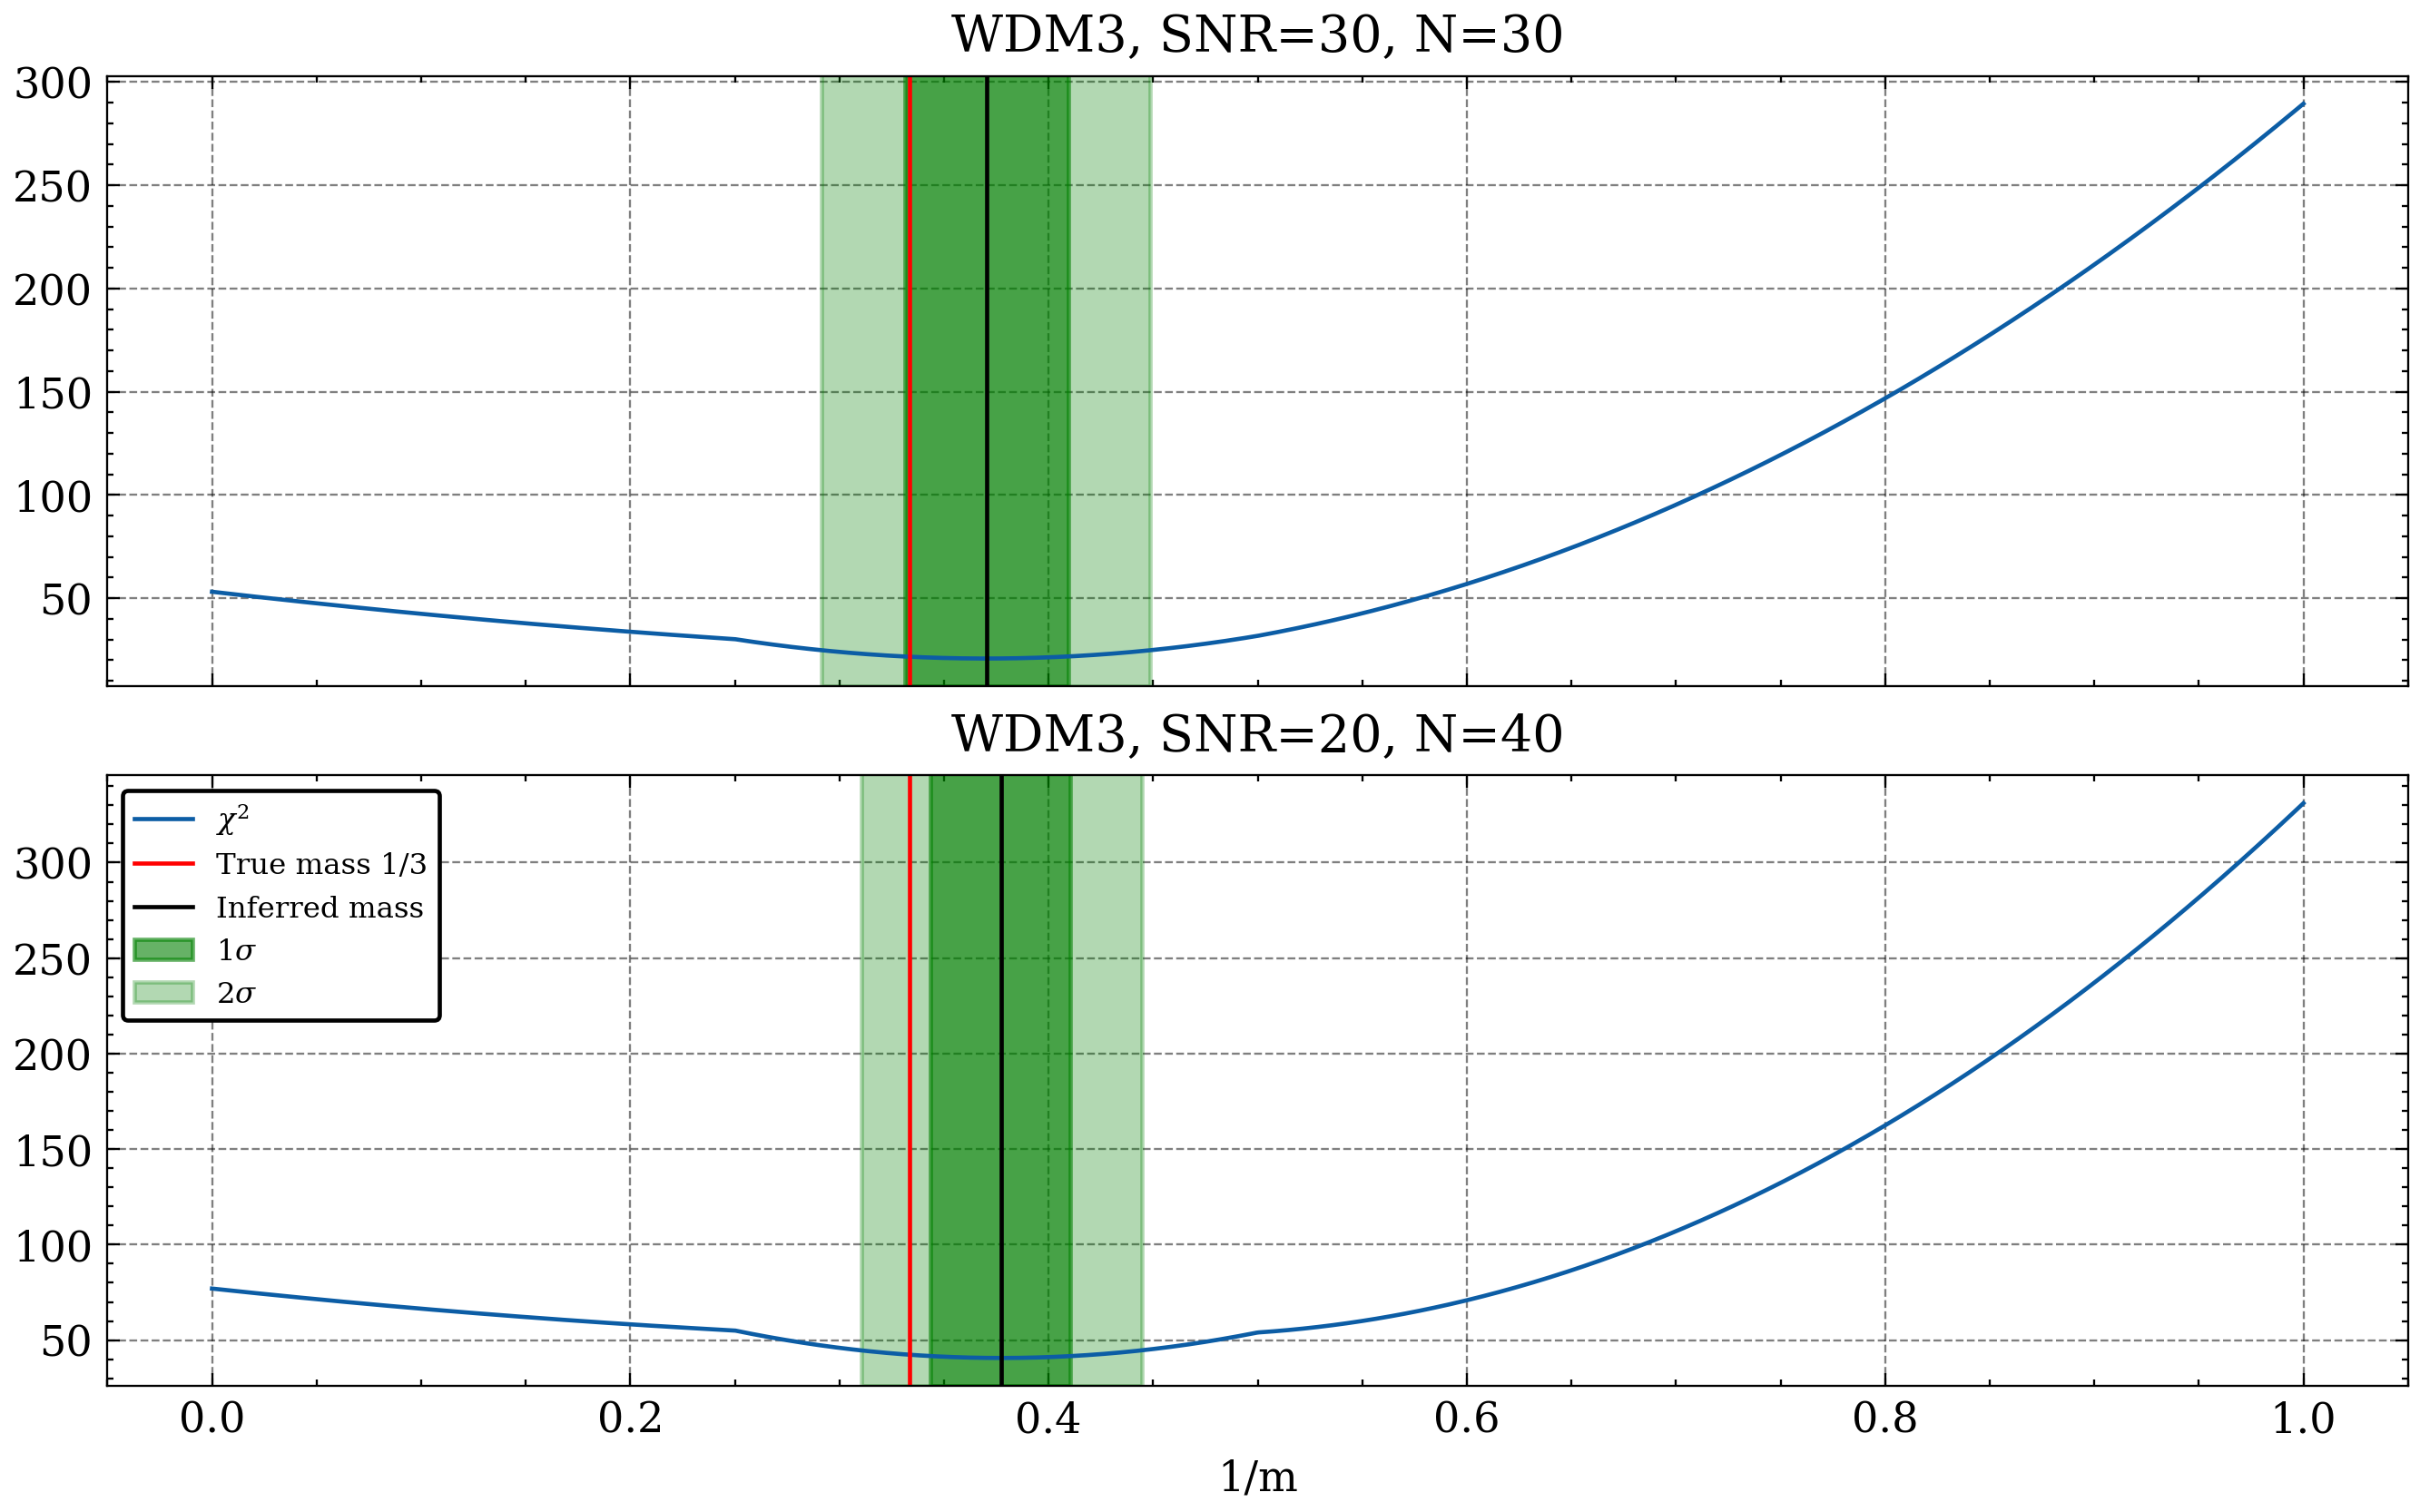
\includegraphics[width=0.8\linewidth]{img/ML/SNR_vs_N.png}
    \caption{Inference predictions on WDM3 for different combinations of SNR and number of targets N.}
    \label{fig: inference snr vs n}
\end{figure}

A common compromise in an observational program with a fixed observational time is between number of targets and exposure time per target, which determines the SNR. In Figure \ref{fig: inference snr vs n} we show how prioritising SNR or the number of targets affects to infered WDM masses on the WDM3 model. In general, we find that increasing the target number leads to slighly tighter confidence regions, while increasing the SNR leads to more accurate constraints. Most crucially, observe how the true model mass is, in both cases, recovered within $2\sigma$.

We now evaluate the constraining power of the approach developed in this work. For that purporse, we assume CDM to be the true DM model and use our fiducial neural network trained on \texttt{SHERWOOD}. We then draw 450 \texttt{SHERWOOD} skewers, corresponding to 30 observed UVES spectra, post-process them with a resolution of 6 km/s, add random Gaussian noise with $\text{SNR}=30$ and use them to run our inference pipeline from section \ref{sec: inference pipeline}. Since the fit depends on the exact draw of ``observed'' skewers, we repeat this process 100 times with a random draw each time to obtain the $2\sigma$ limit distribution.

\begin{figure}
    \centering
    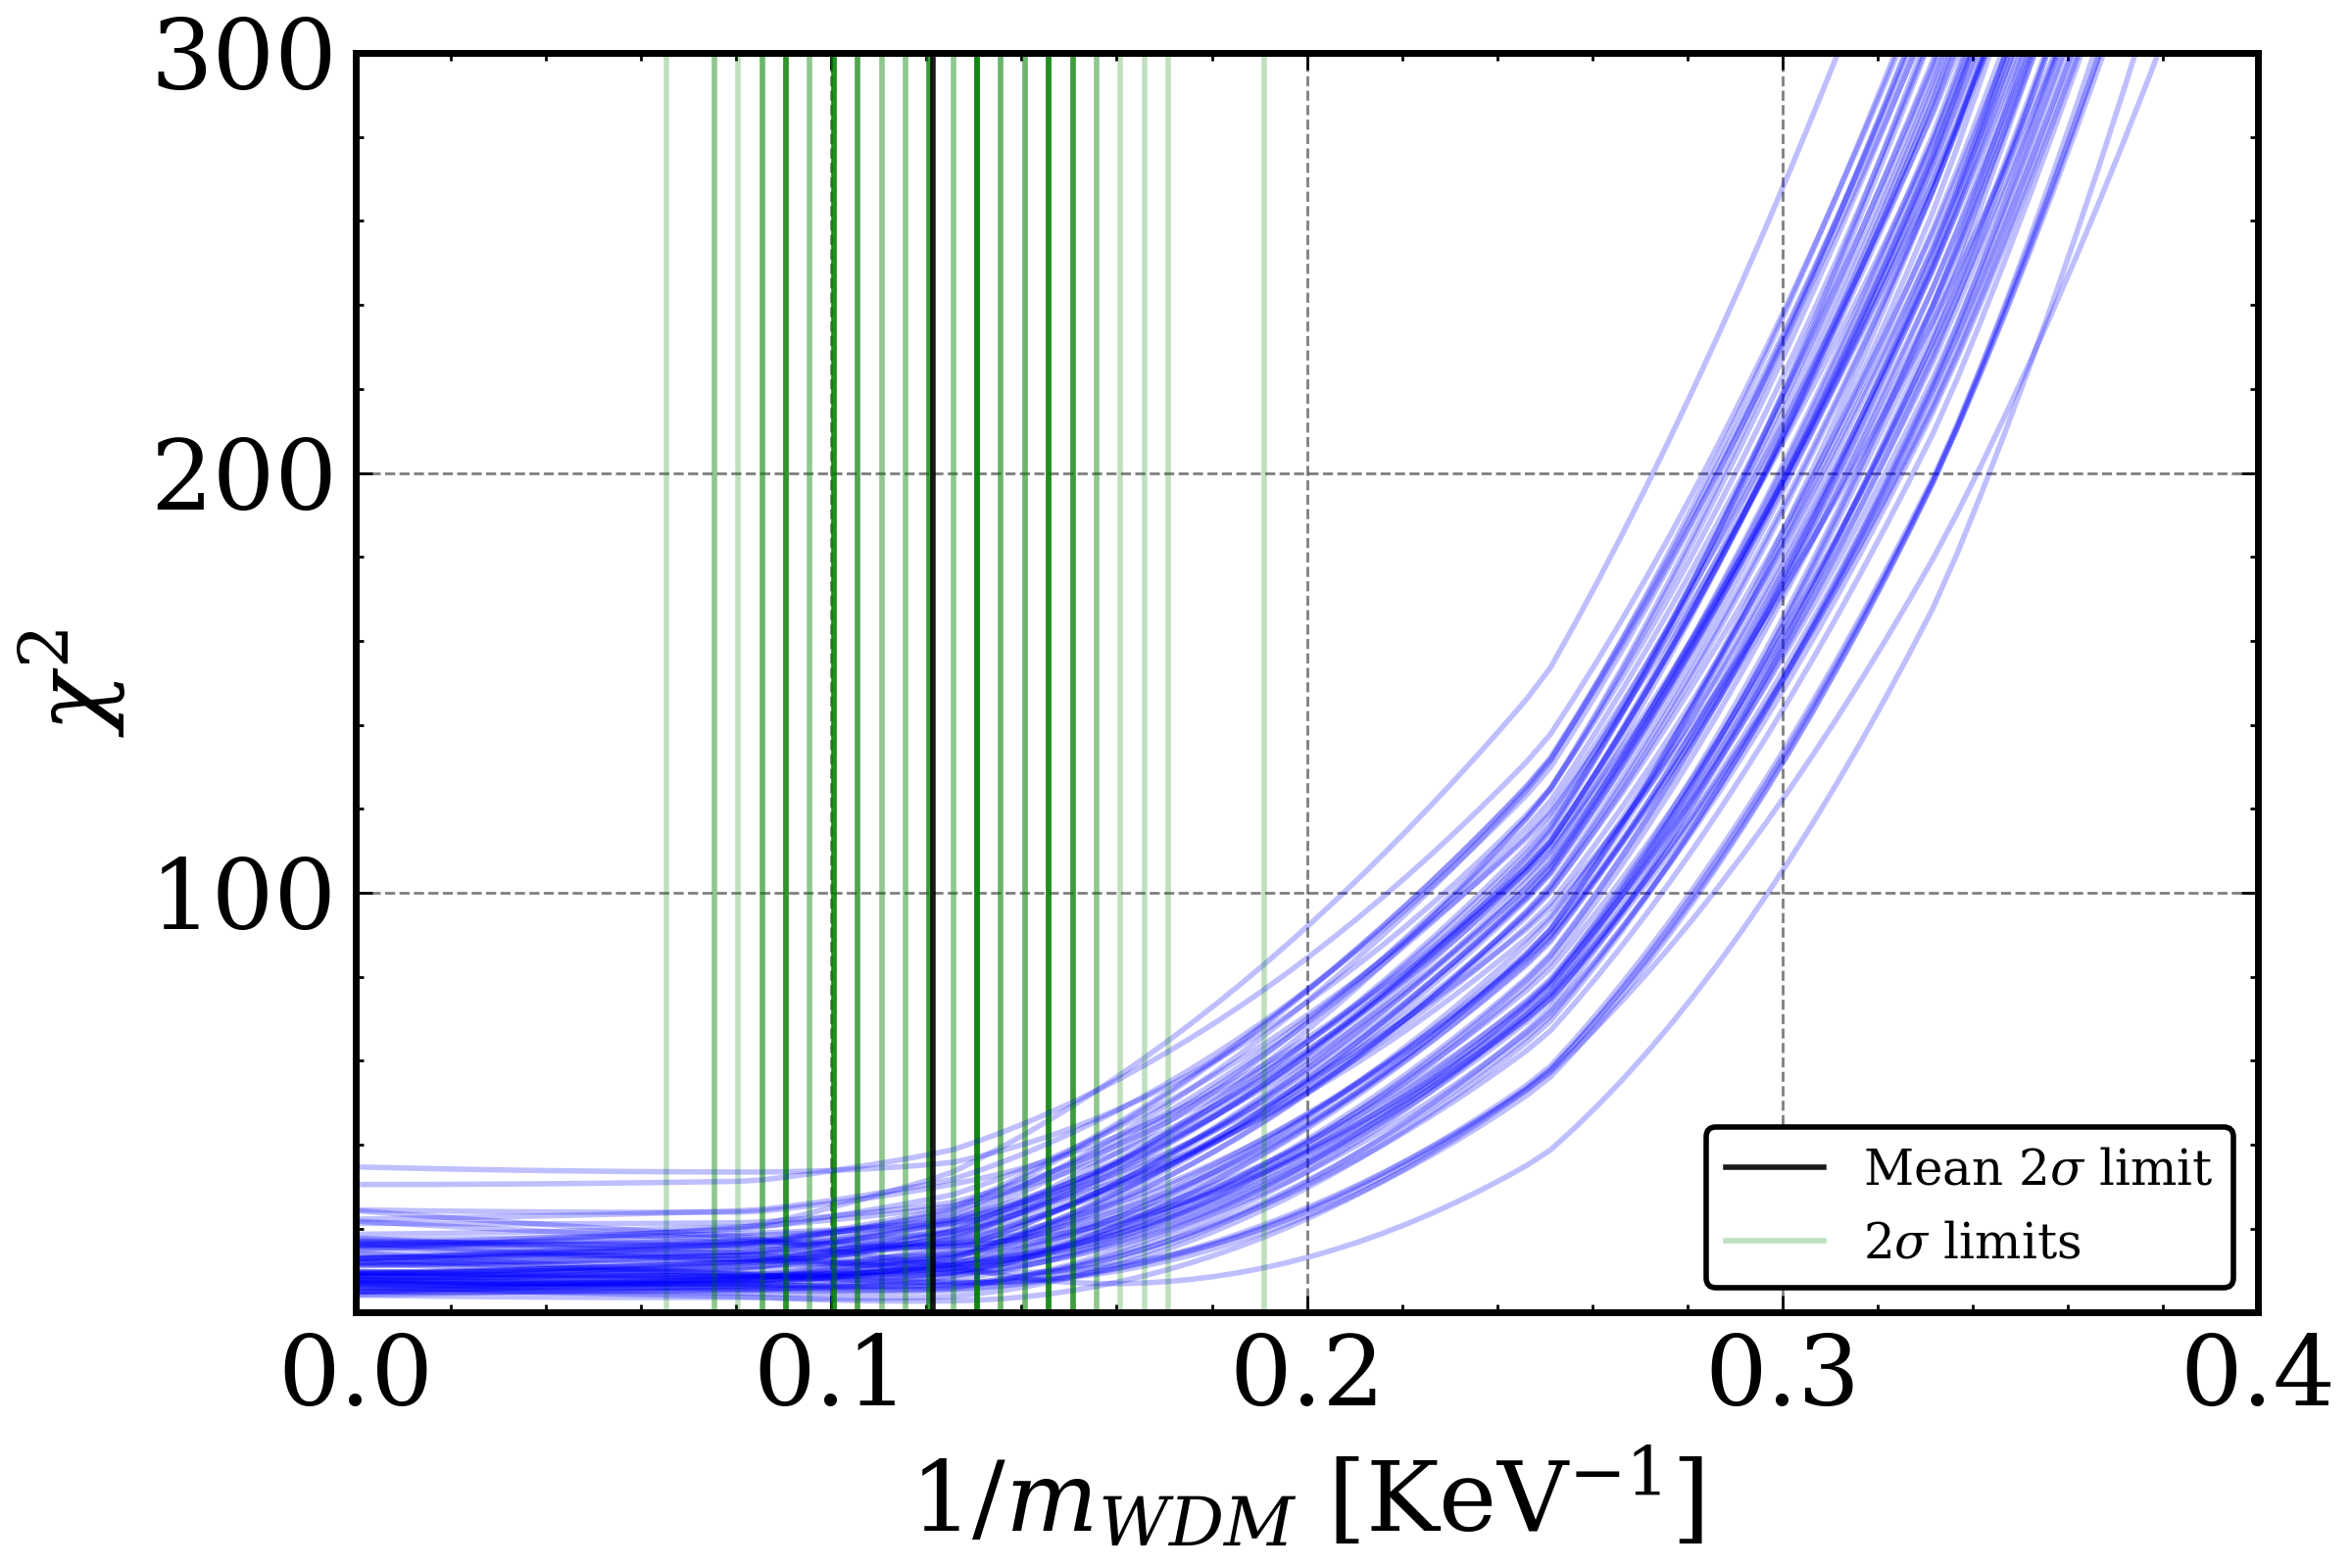
\includegraphics[width=0.8\linewidth]{img/ML/inference_cdm_sherwood.png}
    \caption{The figure shows 100 different $\chi^2$ fits on 450 \texttt{SHERWOOD} CDM skerwers and the $2\sigma$ constraints distribution as we vary the exact obsserved draw.}
    \label{fig: inference cdm sherwood}
\end{figure}
Figure \ref{fig: inference cdm sherwood} shows the distriution of $2\sigma$ limits and the mean $2\sigma$ constraint produced by this process. The mean $2\sigma$ constraint that we report for the inverse mass is $\sim 0.12$ KeV$^{-1}$, or $\sim 8.3$ KeV for the WDM model mass.

\begin{figure}
    \centering
    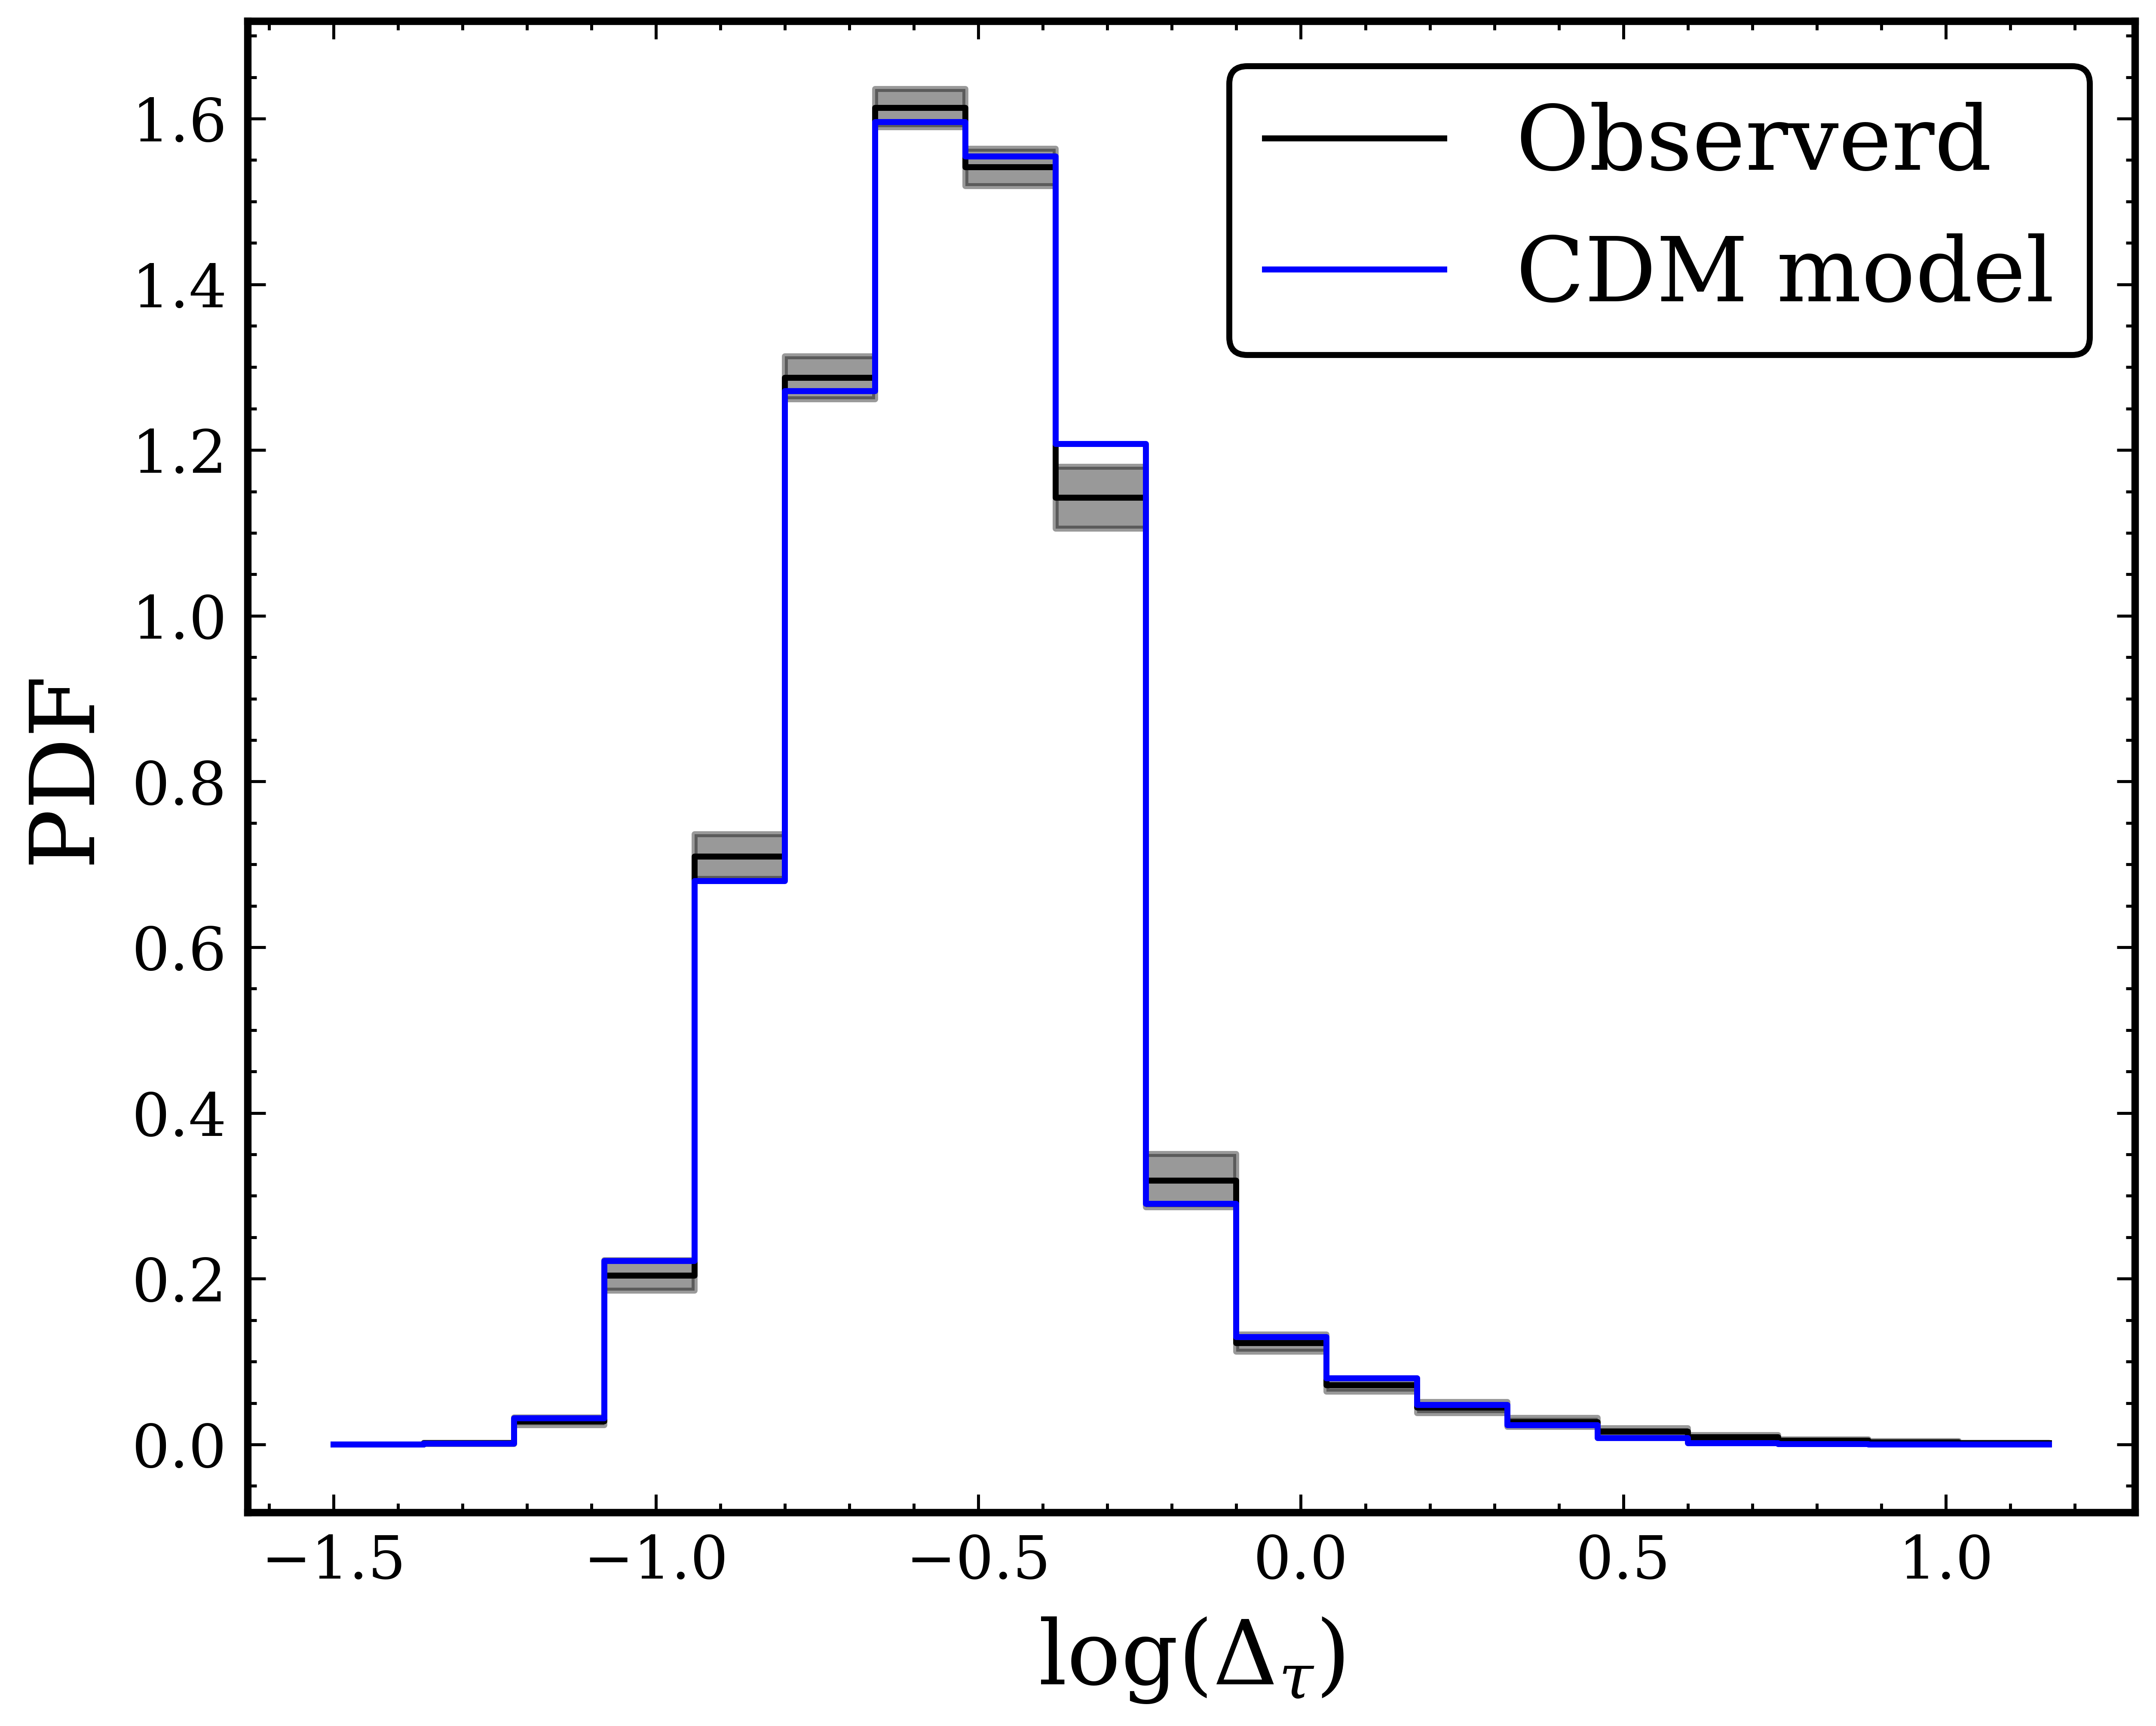
\includegraphics[width=0.6\linewidth]{img/ML/pdf_model_observed.png}
    \caption{An example observed $\Delta_\tau$ PDF recovered using 450 skewers and its uncertainties in black, plotted againt the model CDM PDF, which is the best-fit model in the $\chi^2$ test. }
    \label{fig: inference cdm PDF}
\end{figure}

To confirm that the fitting process works as expected, we plot in Figure \ref{fig: inference cdm PDF} the best fit PDF, which corresponds to the CDM model according to Figure \ref{fig: inference cdm sherwood} and an example recovered PDF from a set of 450 observed skewers. Recall that the uncertainties in the recoved PDF include the sample scatter using bootstrapping as well as the machine learning uncertainties, as we have discussed in setion \ref{sec:recovered statistics}. As expected, the observed PDF in within a $2\sigma$ distance of the model CDM PDF.

In Figure \ref{fig: wdm constraints summary} we summarise in black the current $2\sigma$ state-of-the-art constraint in the literature, using a non-ML approach. In orange, we compare the forecasted constraints from the non-machine learning approach in \cite{sherwood_wdm} to our approach in an equivalent dataset to the one used in section \ref{sec:hires test}. Compared to current limits, our forecasted constraint is a twofold improvemen, from $\sim 4$ to $\sim 8$ KeV. On the same dataset, we forecast our machine learning technique to also outperform the current pipeline in \cite{sherwood_wdm}. As a significant caveat, note that the work in \cite{sherwood_wdm} is a joint analysis not only on WDM but also on thermal parameters of the IGM, cosmological paramters, etc. The aforementioned paper encompasses a larger number of parameters with a more complex and refined approach than this work.


\begin{figure}
    \centering
    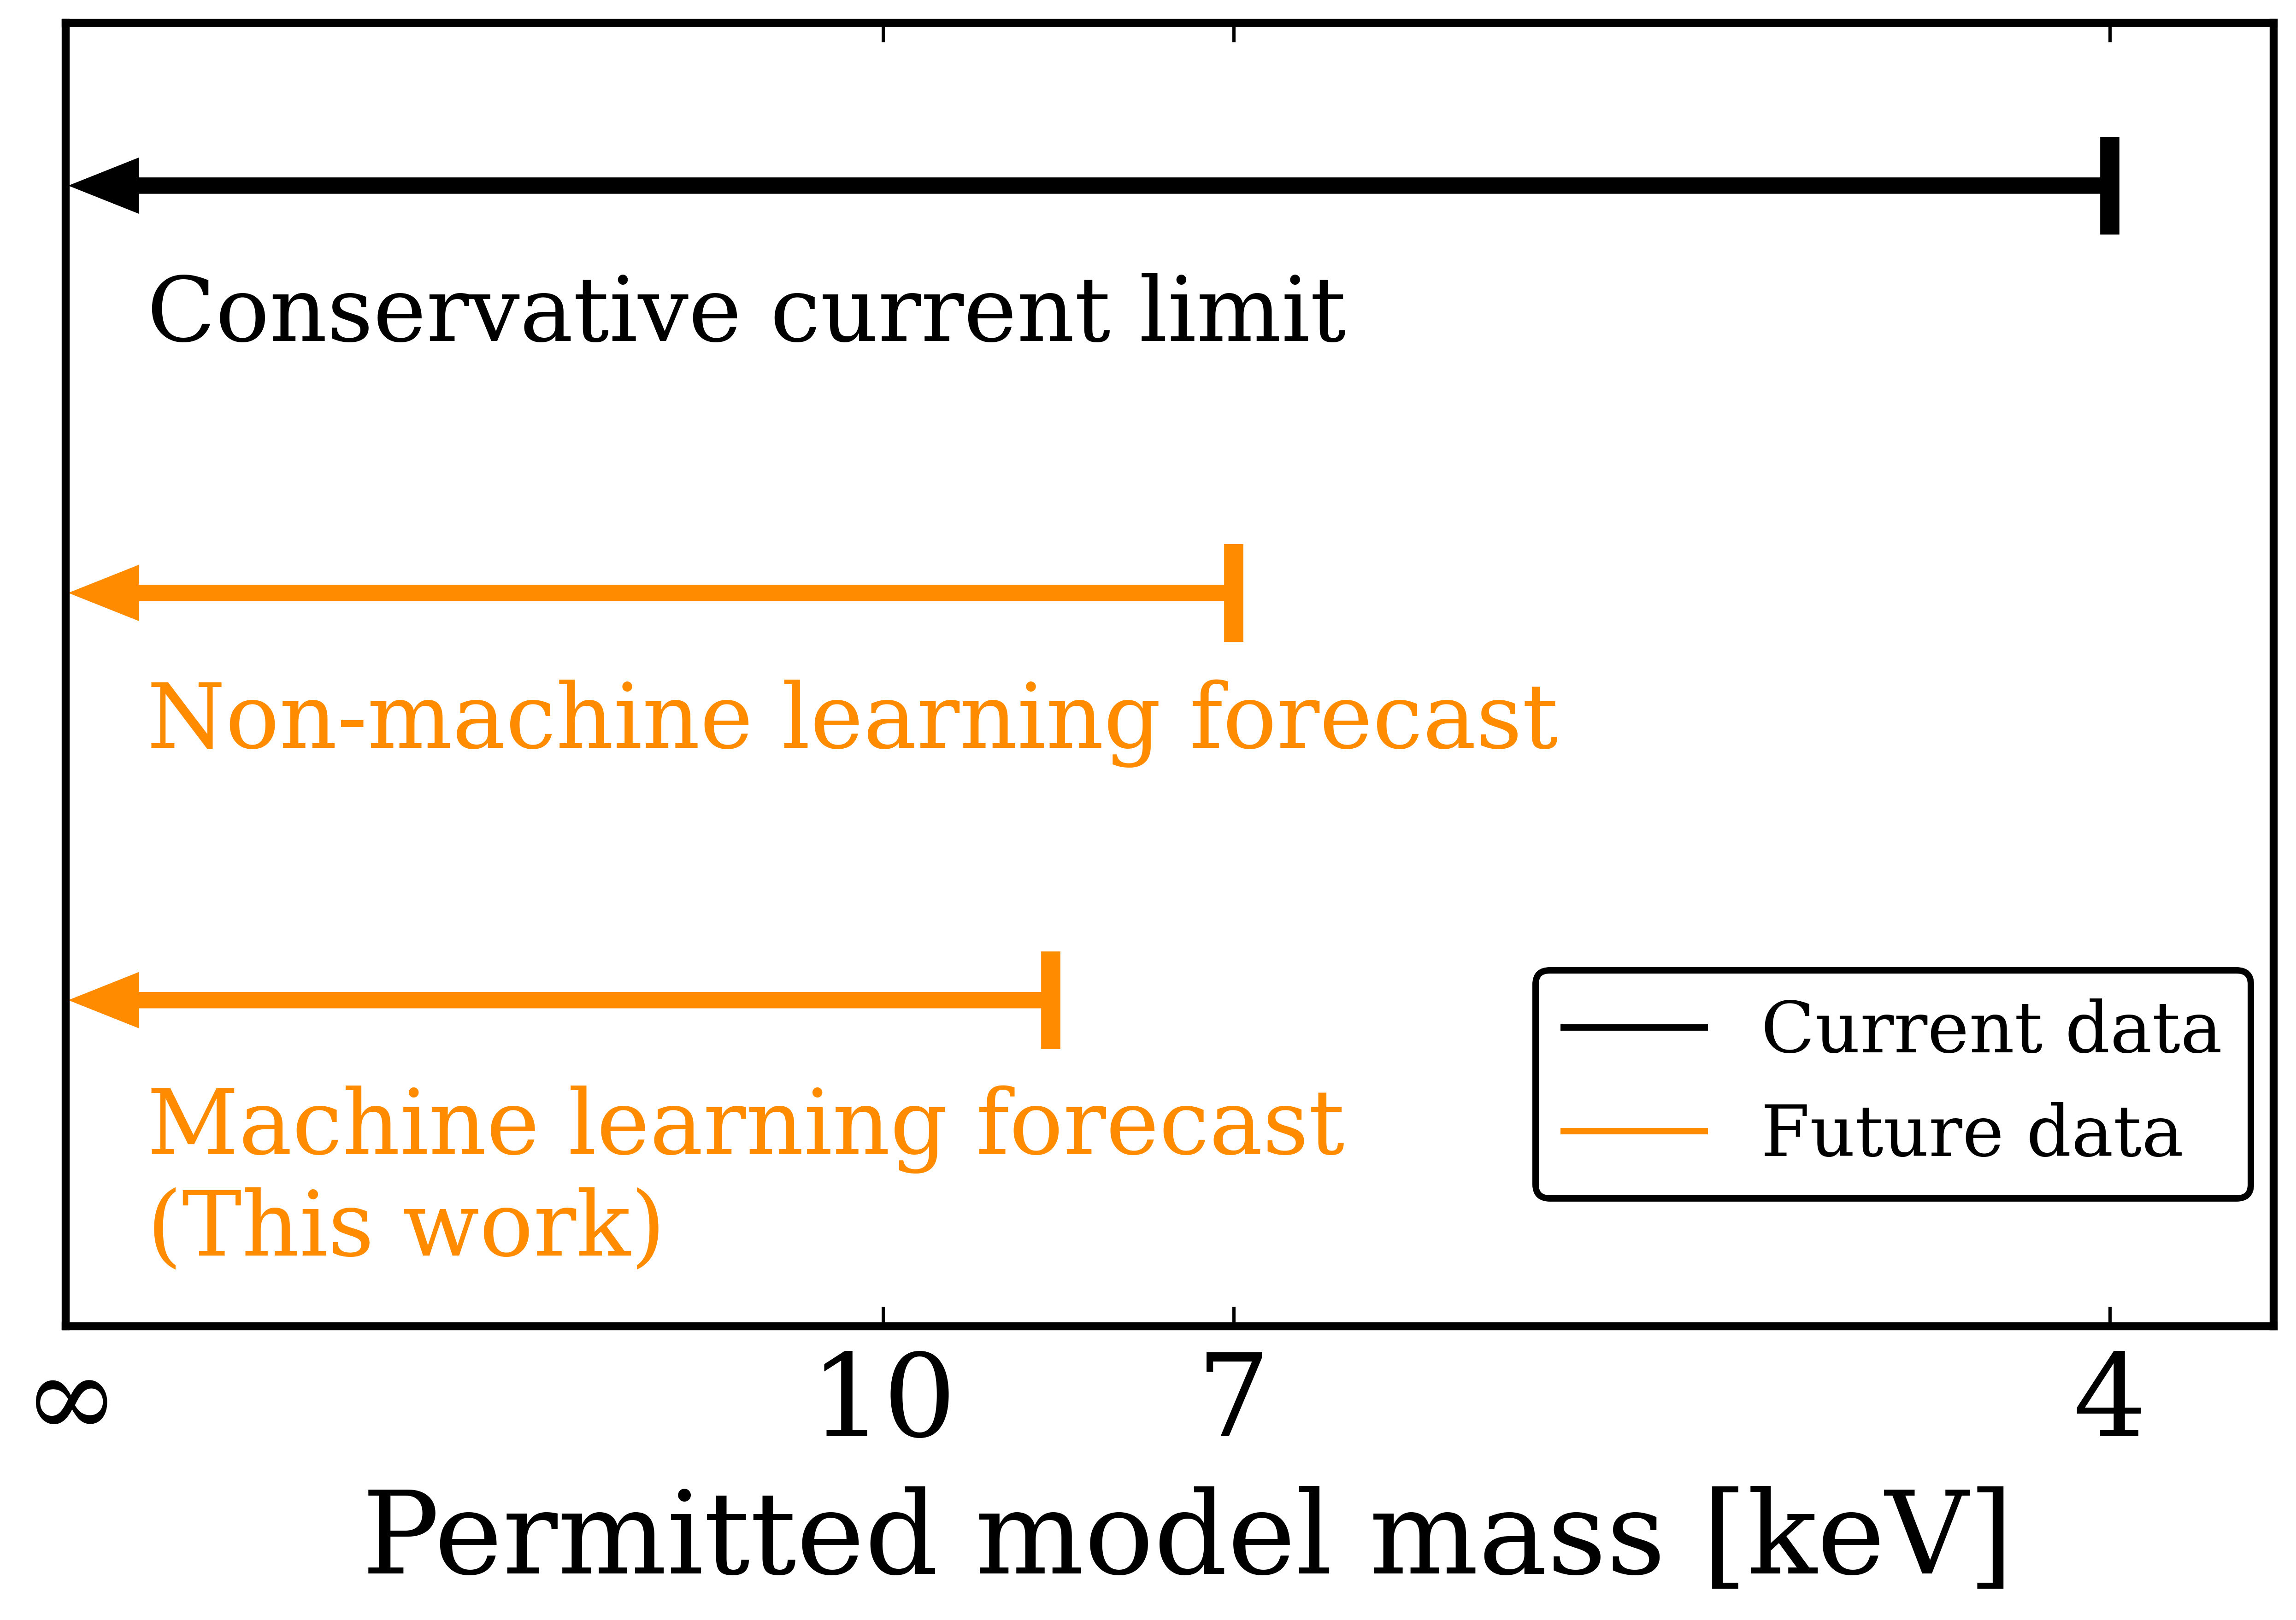
\includegraphics[width=0.6\linewidth]{img/ML/limits_summary.png}
    \caption{Summary $2\sigma$ relic WDM constraints based on \cite{sherwood_wdm} and this work.}
    \label{fig: wdm constraints summary}
\end{figure}













\section{Inference on alternative hydrodynamical codes}
In this section we test our inference pipeline on Nyx, a different hydrodynamical code. We start by discribing in a broad way the differences between the Nyx run used and the Sherwood simulations, and then we use our fiducial neural network trained on the \texttt{SHERWOOD THERMAL} suite to recover the Nyx densities and obtain the corresponding constraints.


\subsection{The Nyx code}
Nyx \cite{Almgren_2013} is an N-body and gas dynamics code for large-scale cosmological simulations. Nyx uses and Adaptive Mesh refinement (AMR) in time and space based on the Eulerian formulation of hydrodynamics, as opposed to the Lagrangian formulation used in the GADGET code emplyed by the Sherwood simulations. We expect Sherwood and Nyx runs to intrinsically show these non-physical differences related to the different hydrodynamical solvers.

In the Nyx code, dark matter is modeled as discrete Lagrangian particles, allowing the code to follow their evolution under gravity effectively. The evolution of its phase space distribution $f$ is given by the collisionless Boltzmann equation

\begin{equation}
    \begin{aligned}\frac{\partial f}{\partial t}+\frac{1}{ma^2}\mathbf{p}\cdot\nabla f-m\nabla\phi\cdot\frac{\partial f}{\partial\mathbf{p}}=0\end{aligned}
\end{equation}
where $m$ and $\mathbf{p}$ are mass and momentum and $\phi$ is the gravitational potential. $a$ is the sacale factor, obtained by using a second-order Runge-Kutta solver.
Nyx solves this phase space evolution of $f$ by sampling its distribution and evolving the particles as an N-body system. The gravitational potential is obtained by solving the Poisson equation

\begin{equation}
    \nabla^2\phi(\mathbf{x},t)=\frac{4\pi G}{a}(\rho_b+\rho_{dm}-\rho_0)
\end{equation}
where $\rho_0$ is the mean density, $\rho_b$ the baryonic density and $\rho_{dm}$ the dark matter density.
Dark matter particles are gravitationally coupled to a baryonic fluid, which is treated as an inviscid ideal gas. The gas is described by a state vector $\mathbf{U}=(\rho_b,a\rho_bU,a^2\rho_bE,a^2\rho_be)$ where $U$ is the peculiar proper baryonic velocity, $e$ the internal energy, and $E$ the total energy.
The hydrodynamical equations are approximate by a Riemann solver and can be written in the form
\begin{equation}
    \frac{\partial\mathbf{U}}{\partial t}=-\nabla\cdot\mathbf{F}+S_e+S_g+S_{HC},
\end{equation}
where $F$ is the flux vector, $S_g$ the gravity source term, $S_{HC}$ the heating and cooling term, and $S_e$ the internal energy flux.

In the rest of this section, we consider 3 Nyx runs at $z=4.4$ using CDM and 20h$^{-1}$cMpc boxes. The 3 runs different in the different reionization hisory, and are labelled by the end of reionization redshifts of $z_\mathrm{re}=6,7,8$. Each skewer has 1024 pixels. In Figure \ref{fig: nyx skewer} show an example Lyman-$\alpha$ skewer for the Nyx run with $z_\mathrm{re}=6$.


\begin{figure}
    \centering
    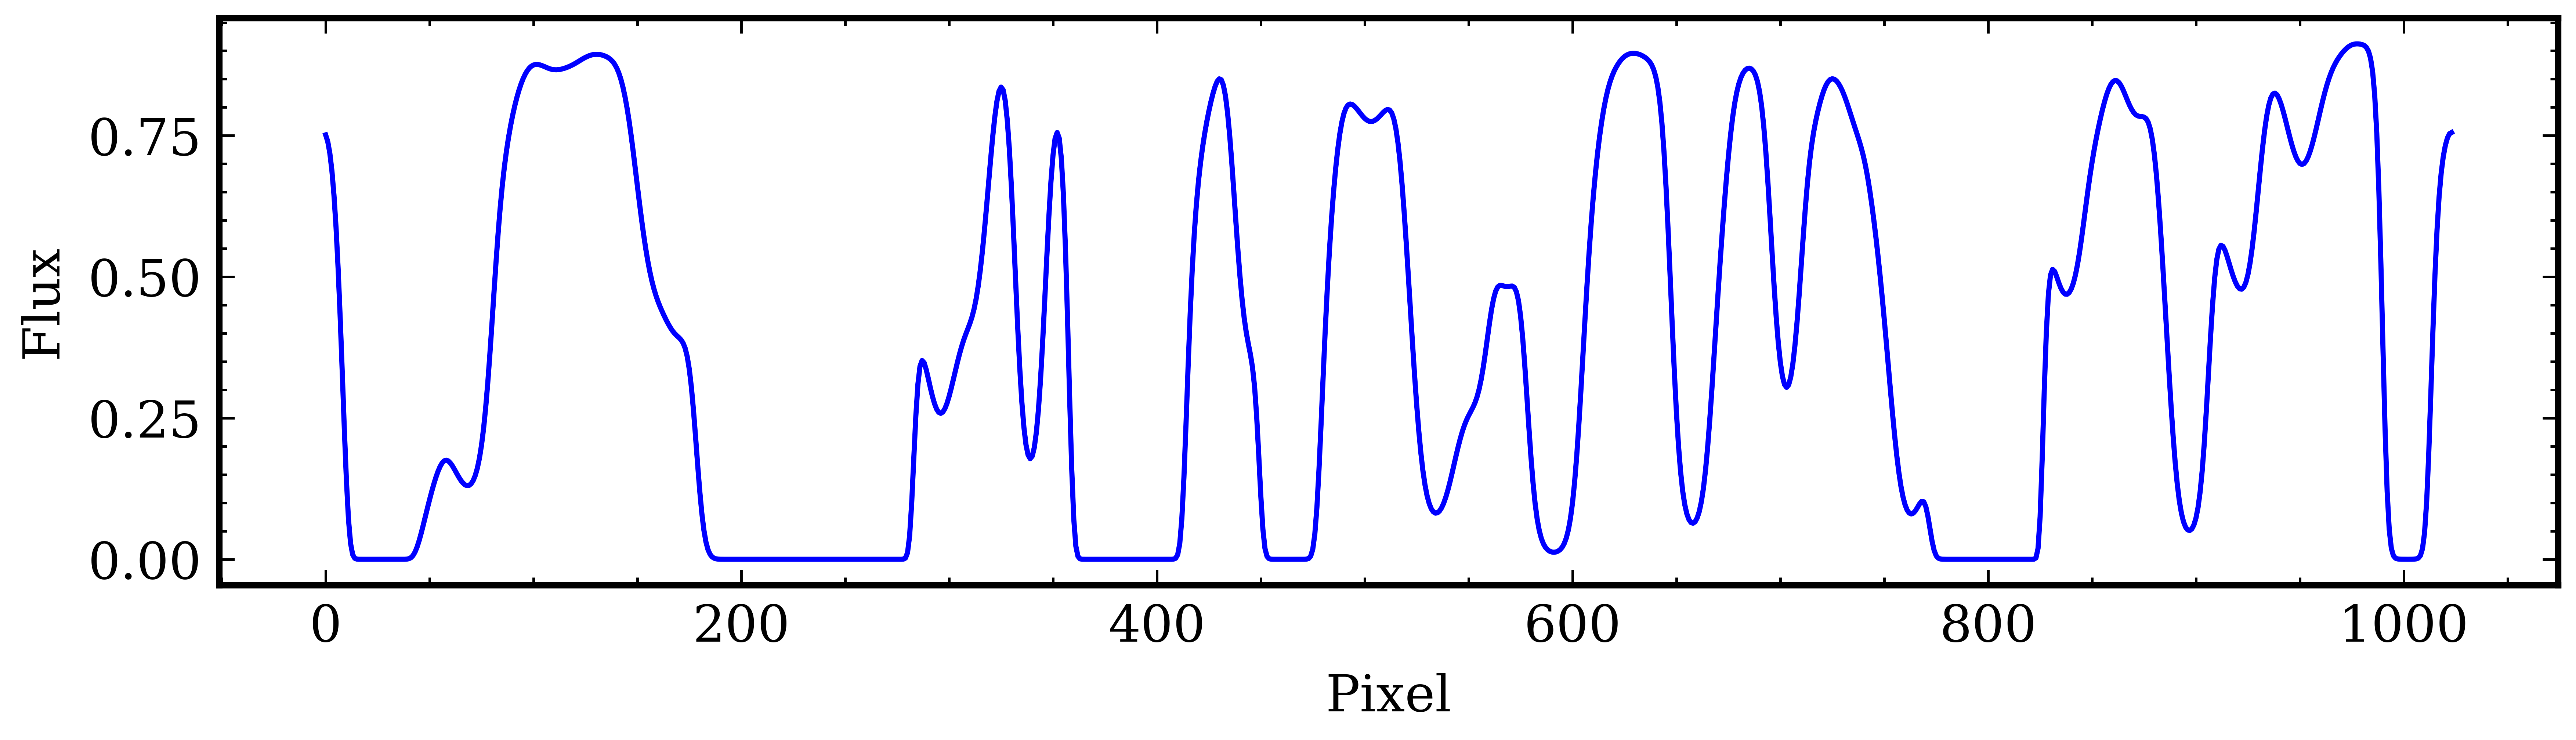
\includegraphics[width=0.8\linewidth]{img/ML/nyx_skewer.png}
    \caption{A typical Lyman-$\alpha$ skewer obtained from the Nyx runs with $z_\mathrm{re}=6$ at $z=4.4$.}
    \label{fig: nyx skewer}
\end{figure}
Since we want to test our inference pipeline, in this test we want to be as agnostic as possible about the nature of our ``observed'' Nyx spectra. If real data is observed, we would, a priori, have no information on the exact thermal history that has led to the observed field. A similar situation occurs with the Nyx runs. Our \texttt{SHERWOOD THERMAL} dataset constrains thermal models, but we have a priori no guarantee that they match the Nyx runs that we are analysing. In fact, we know that this is not the case. We visually explore the difference between the \texttt{Nyx} and \texttt{SHERWOOD THERMAL} runs, we plot the 2D distribution of pixels in the temperature-density plane. We show the result in Figure \ref{fig: nyx TD}, comparing the \texttt{Nyx} CDM run $z_\mathrm{re}=6$ to the \texttt{SHERWOOD THERMAL} CDM runs. The top panel shows the $95\%$ contours in red and black colors. The bottom ponel shows the temperature distribution at the mean density value. As can be obsered, the \text{Nyx} does not fit any of the runs in our training dataset.


\begin{figure}
    \centering
    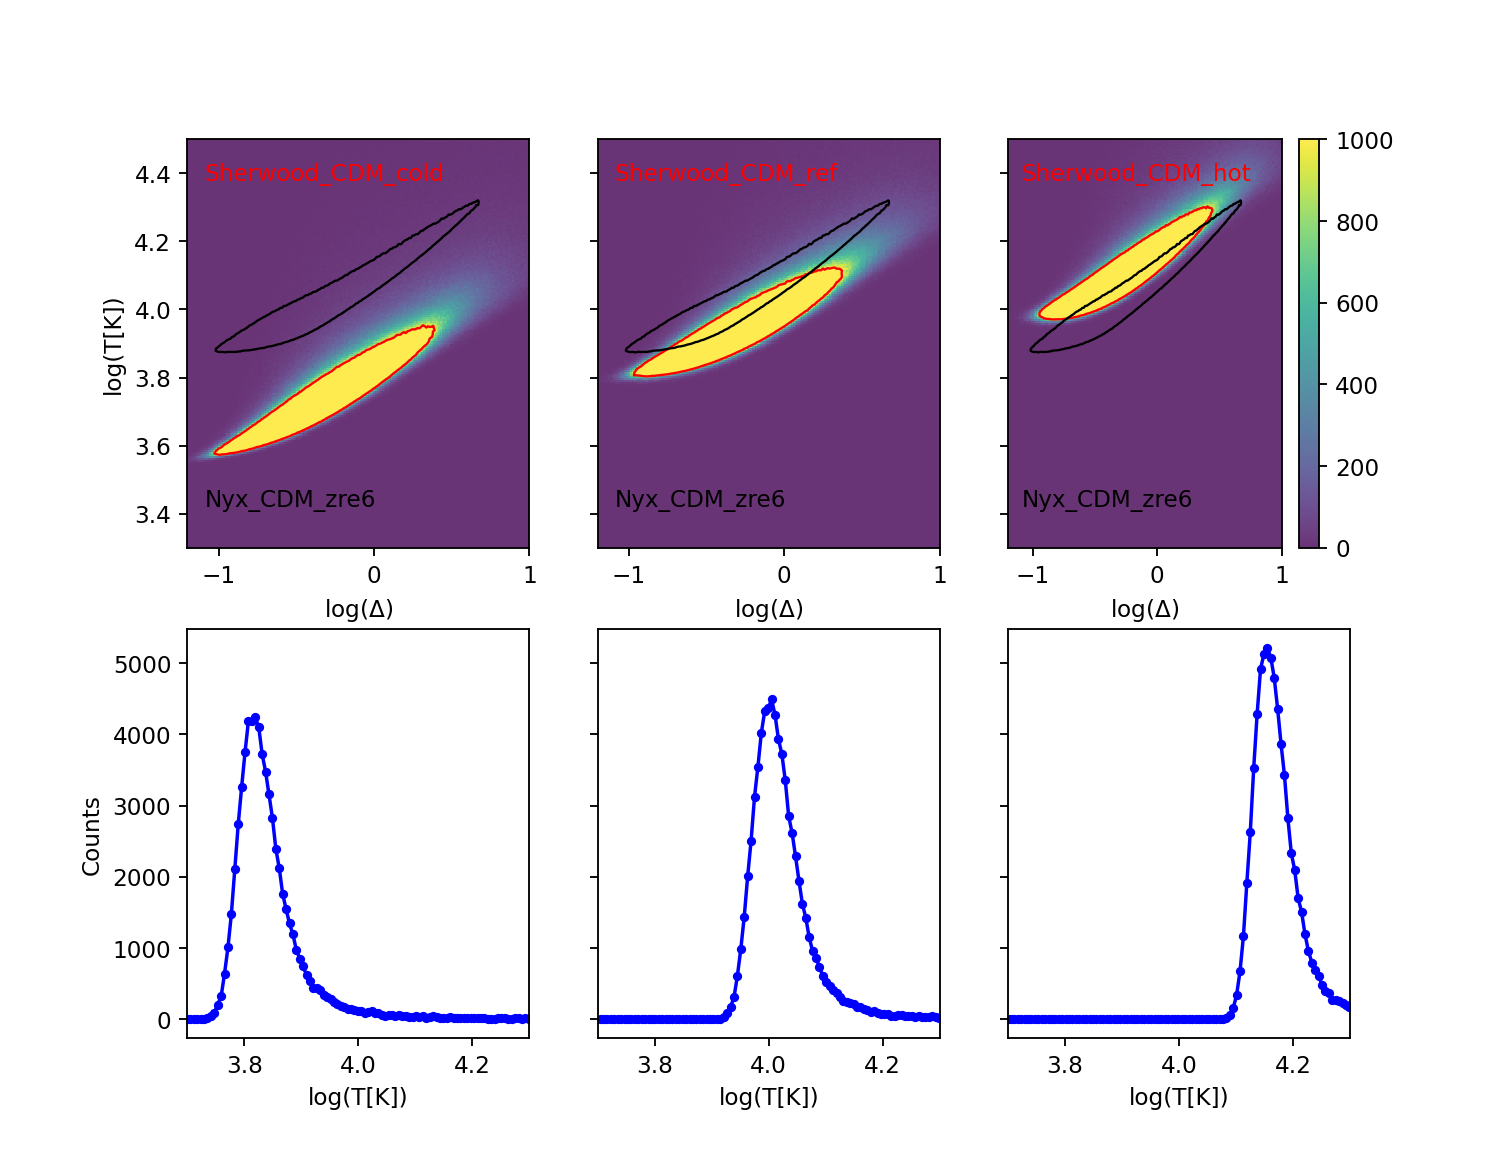
\includegraphics[width=0.99\linewidth]{img/ML/TD_plane_nyx_sher.png}
    \caption{The 2D distribution of pixels in the temperature-density plane comparing the \texttt{Nyx} CDM run $z_\mathrm{re}=6$ to the \texttt{SHERWOOD THERMAL} CDM runs. The top panel shows the $95\%$ contours in red and black colors. The bottom ponel shows the temperature distribution at the mean density value. As can be obsered, the \text{Nyx} does not fit any of the runs in our training dataset.}
    \label{fig: nyx TD}
\end{figure}

\subsection{Inference test on Nyx Lyman-alpha skewers}
We begin by evaluating the performance of our fiducial neural network with frozen weights trained on \texttt{SHERWOOD THERMAL} when predicting of skewers generated by the \texttt{Nyx} code. In Figure \ref{fig: nyx violin} we show a violin plot with the $1\sigma$ residues distribution as defined in Equation \ref{eq: residuals}. Values in the range $[0,1]$ correspond to pixels that have been succesfully recovered within a $1\sigma$ accuracy. Observer how the models with earlier reionization ($z_\mathrm{re}=7$ and $z_\mathrm{re}=8$), which have lower temperatures, have a higher recovery rate. This is likely due to the fact that our training data set contains more WDM models close to CDM, and we know that loss WDM masses and low temperate have a degenerate effect on the Lyman-$\alpha$ forest. In general, we note that the $\geq 75 \%$ of the pixels are correctly recovered. Even is the performance is slightly degraded compared to the \text{SHERWOOD THERMAL} validation, as expected, this is a strong indication that the neural network has learnt the relevant physical relations, and not potential simulation-specific correlations.

\begin{figure}
    \centering
    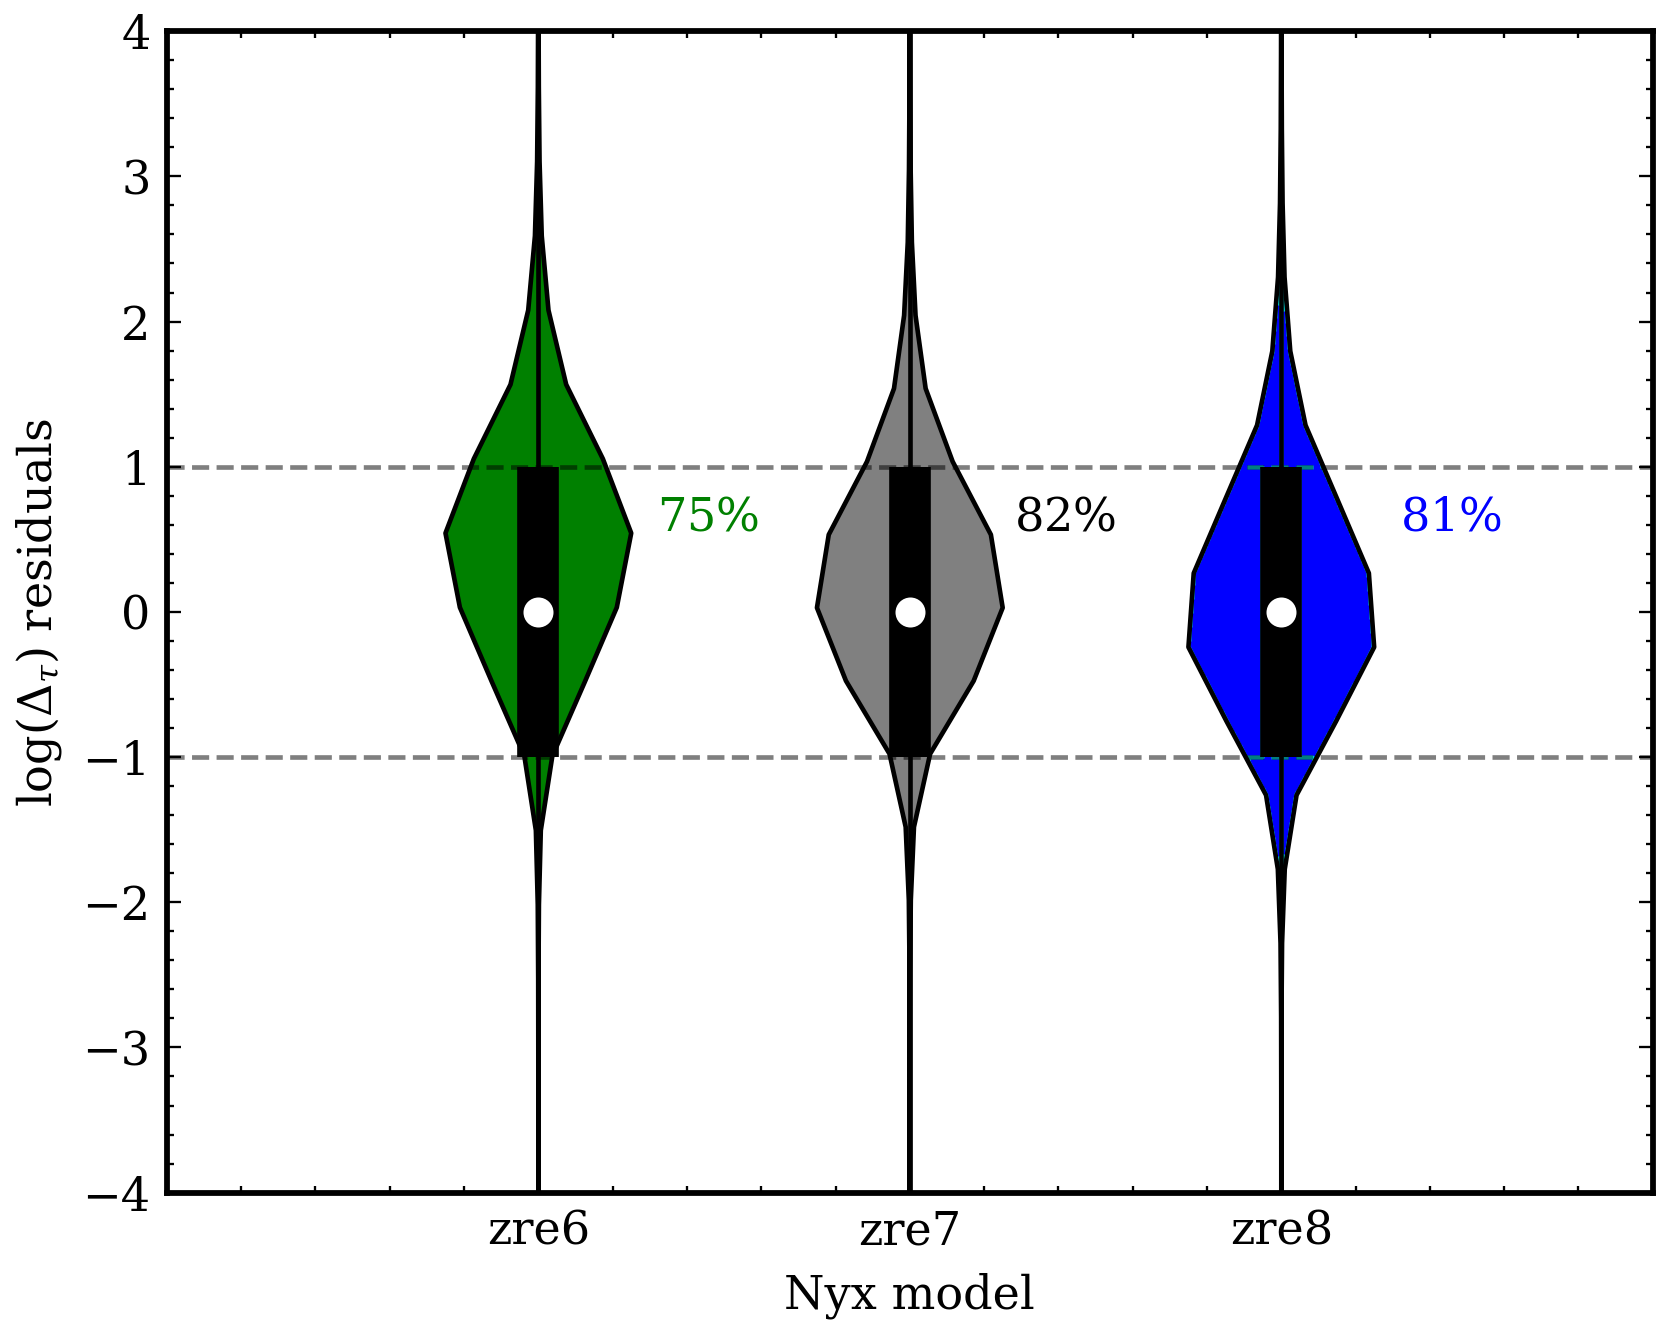
\includegraphics[width=0.8\linewidth]{img/ML/violin_nyx.png}
    \caption{Violin plot with the $1\sigma$ residues distribution as defined in Equation \ref{eq: residuals}. Values in the range $[0,1]$ correspond to pixels that have been succesfully recovered within a $1\sigma$ accuracy. Observer how the models with earlier reionization ($z_\mathrm{re}=7$ and $z_\mathrm{re}=8$), which have lower temperatures, have a higher recovery rate. This is likely due to the fact that our training data set contains more WDM models close to CDM, and we know that loss WDM masses and low temperate have a degenerate effect on the Lyman-$\alpha$ forest. In general, we note that the $\geq 75 \%$ of the pixels are correctly recovered.}
    \label{fig: nyx violin}
\end{figure}
We then run the same inference pipeline for the $z_\mathrm{re}=6$ model as we did in section \ref{sec:hires test} with a single major difference. Since we know that the \texttt{Nyx} runs do not fit any of our thermal models (and the same circumstance will occur when using real observations), we need to utilise the fiducial neural network trained on multiple thermal modes, \texttt{SHERWOOD THERMAL}. Additionally, when fitting the recovered $\Delta_\tau$ PDF to each model PDF, we will have 3 different $\chi^2$ curves for each one of the thermal models $\{\mathrm{ref}, \mathrm{hot}, \mathrm{cold} \}$. To avoid a joint optimization problem and constraining the thermal history on top of the WDM mass (which is out of the scoop of this work, and also unrealisitc since we are not using a fine thermal model grid), we will select the thermal model that minimises the $\chi^2$ value, that is
\begin{equation}\label{eq: chi thermal def}
    \mathrm{min}_{t,m} \, \, \chi^2(t,m),
\end{equation}
where $t\in \{\mathrm{ref}, \mathrm{hot}, \mathrm{cold} \}$ and $m$ labels the continously interpolatted inverse warm dark matter mass. We compute $\chi^2(t,m)$ and find that the ref and hot model produce similar $\chi^2$ values, while the cold model has $\chi^2 \sim 1000$, as expected from Figure \ref{fig: nyx TD}. Both the ref and hot models produce a similar $2\sigma$ lower bound on the WDM mass: $m_{\mathrm{WDM}} \gtrsim 10$ KeV. Compared to section \ref{sec:hires test}, the results are fairly similar, showcasing the robustness of our approach.
































\section{WDM constraints from SQUAD DR1 observational data}\label{sec:inference squad}
We begin applying our density recovery and WDM mass inference pipeline to a set of 6 observed quasar sightlines from the SQUAD DR1 survey \cite{Murphy_2018}. Since we are working with observational data, we will always train the model with the complete \texttt{SHERWOOD THERMAL} dataset that includes varied thermal histories and WDM masses. Note that since we are not trying to cosntraint the thermal history (or other parameters that can affect the Lyman-$\alpha$ forest), we should ideally use a training set that includes as much variation as possible to make sure the neural network can perform in a scenario where we ignore the true thermal history.

Our SQUAD DR1  data consists of 6 Lyman-$\alpha$ sightlines of size 20h$^{-1}$cMpc with varied SNR (see table \ref{tab: squad dr1}), observed with the Ultraviolet and Visual Echelle Spectrograph (UVES) on the European Southern Observatory’s Very Large Telescope, which has an average resolution of $\mathrm{FWHM}\approx 6$km s$^{-1}$. We consider sightlines centred at $z=4.4$ for this specific application. Since each quasar has its own noise level, we retrain the same fiducial architecture with the corresponding noise level before the prediction step.

\begin{table}
    \caption[]{List of the SQUAD DR1 sightlines used, see \cite{Murphy_2018} for the reduction details, together with their emission redshift and the average continuum SNR.     
    All sightlines are 20h$^{-1}$cMpc and centered at $z=4.4$.}
    \label{tab: squad dr1}
   $$ 
       \begin{array}{p{0.4\linewidth}cc}
          \hline
          \noalign{\smallskip}
          SQUAD DR1 name &  z_{\mathrm{em.}} & \mathrm{SNR} \\ 
          \noalign{\smallskip}
          \hline
          \noalign{\smallskip}
          J004054 &4.976  & 33    \\
          J021043           &4.65   &25\\
          J025019     &4.77   &     12      \\
          J030722     &4.728        &   50          \\
          J033829 &  5.032             &  14         \\
          J145147  & 4.763                 &  100         \\
          \noalign{\smallskip}
          \hline
       \end{array}
   $$ 
 \end{table}


We are then set to predict the recovered density fields for easch sightline. Figure \ref{fig: squad pred} shows all our SQUAD DR1 skewers togethet with the recoved $\Delta_\tau$ field.

\begin{figure}
    \centering
    \includegraphics[width=0.7\linewidth]{img/ML/SQUAD_pred.png}
    \caption{All 6 sightlines from the SQUAD DR1 sample in Table \ref{tab: squad dr1}. As can be seen, the noise levels vary, depending on the exposure time to the target. All sightlines are 20h$^{-1}$cMpc and centered at $z=4.4$. We show the recovered density field by our fiducial architecture trained on \texttt{SHERWOOD THERMAL} and retrained with the noise specifications of each target.}
    \label{fig: squad pred}
\end{figure}

We now compute the $\chi^2(t,m)$ for all 3 thermal models, which are minimised for the respective CDM run as expected, and find that the thermal model producing a minimal $\chi^2$ is the cold. In Figure \ref{fig: squad chi pdf} we show, in the left panel, all 3 $\chi^2$ curves as a function of the WDM mass. The right panel shows the recovered $\Delta_\tau$ PDF from the SQUAD DR1 sample together with the best-fit model, corresponding to the CDM cold \texttt{SHERWOOD THERMAL} model. Using the best-fit thermal model, we find a lower bound on the WDM mass of $m_{\mathrm{WDM}} \gtrsim 3.8$ KeV.


\begin{figure}
    \centering
    \begin{subfigure}[b]{0.53\textwidth}
        \centering
            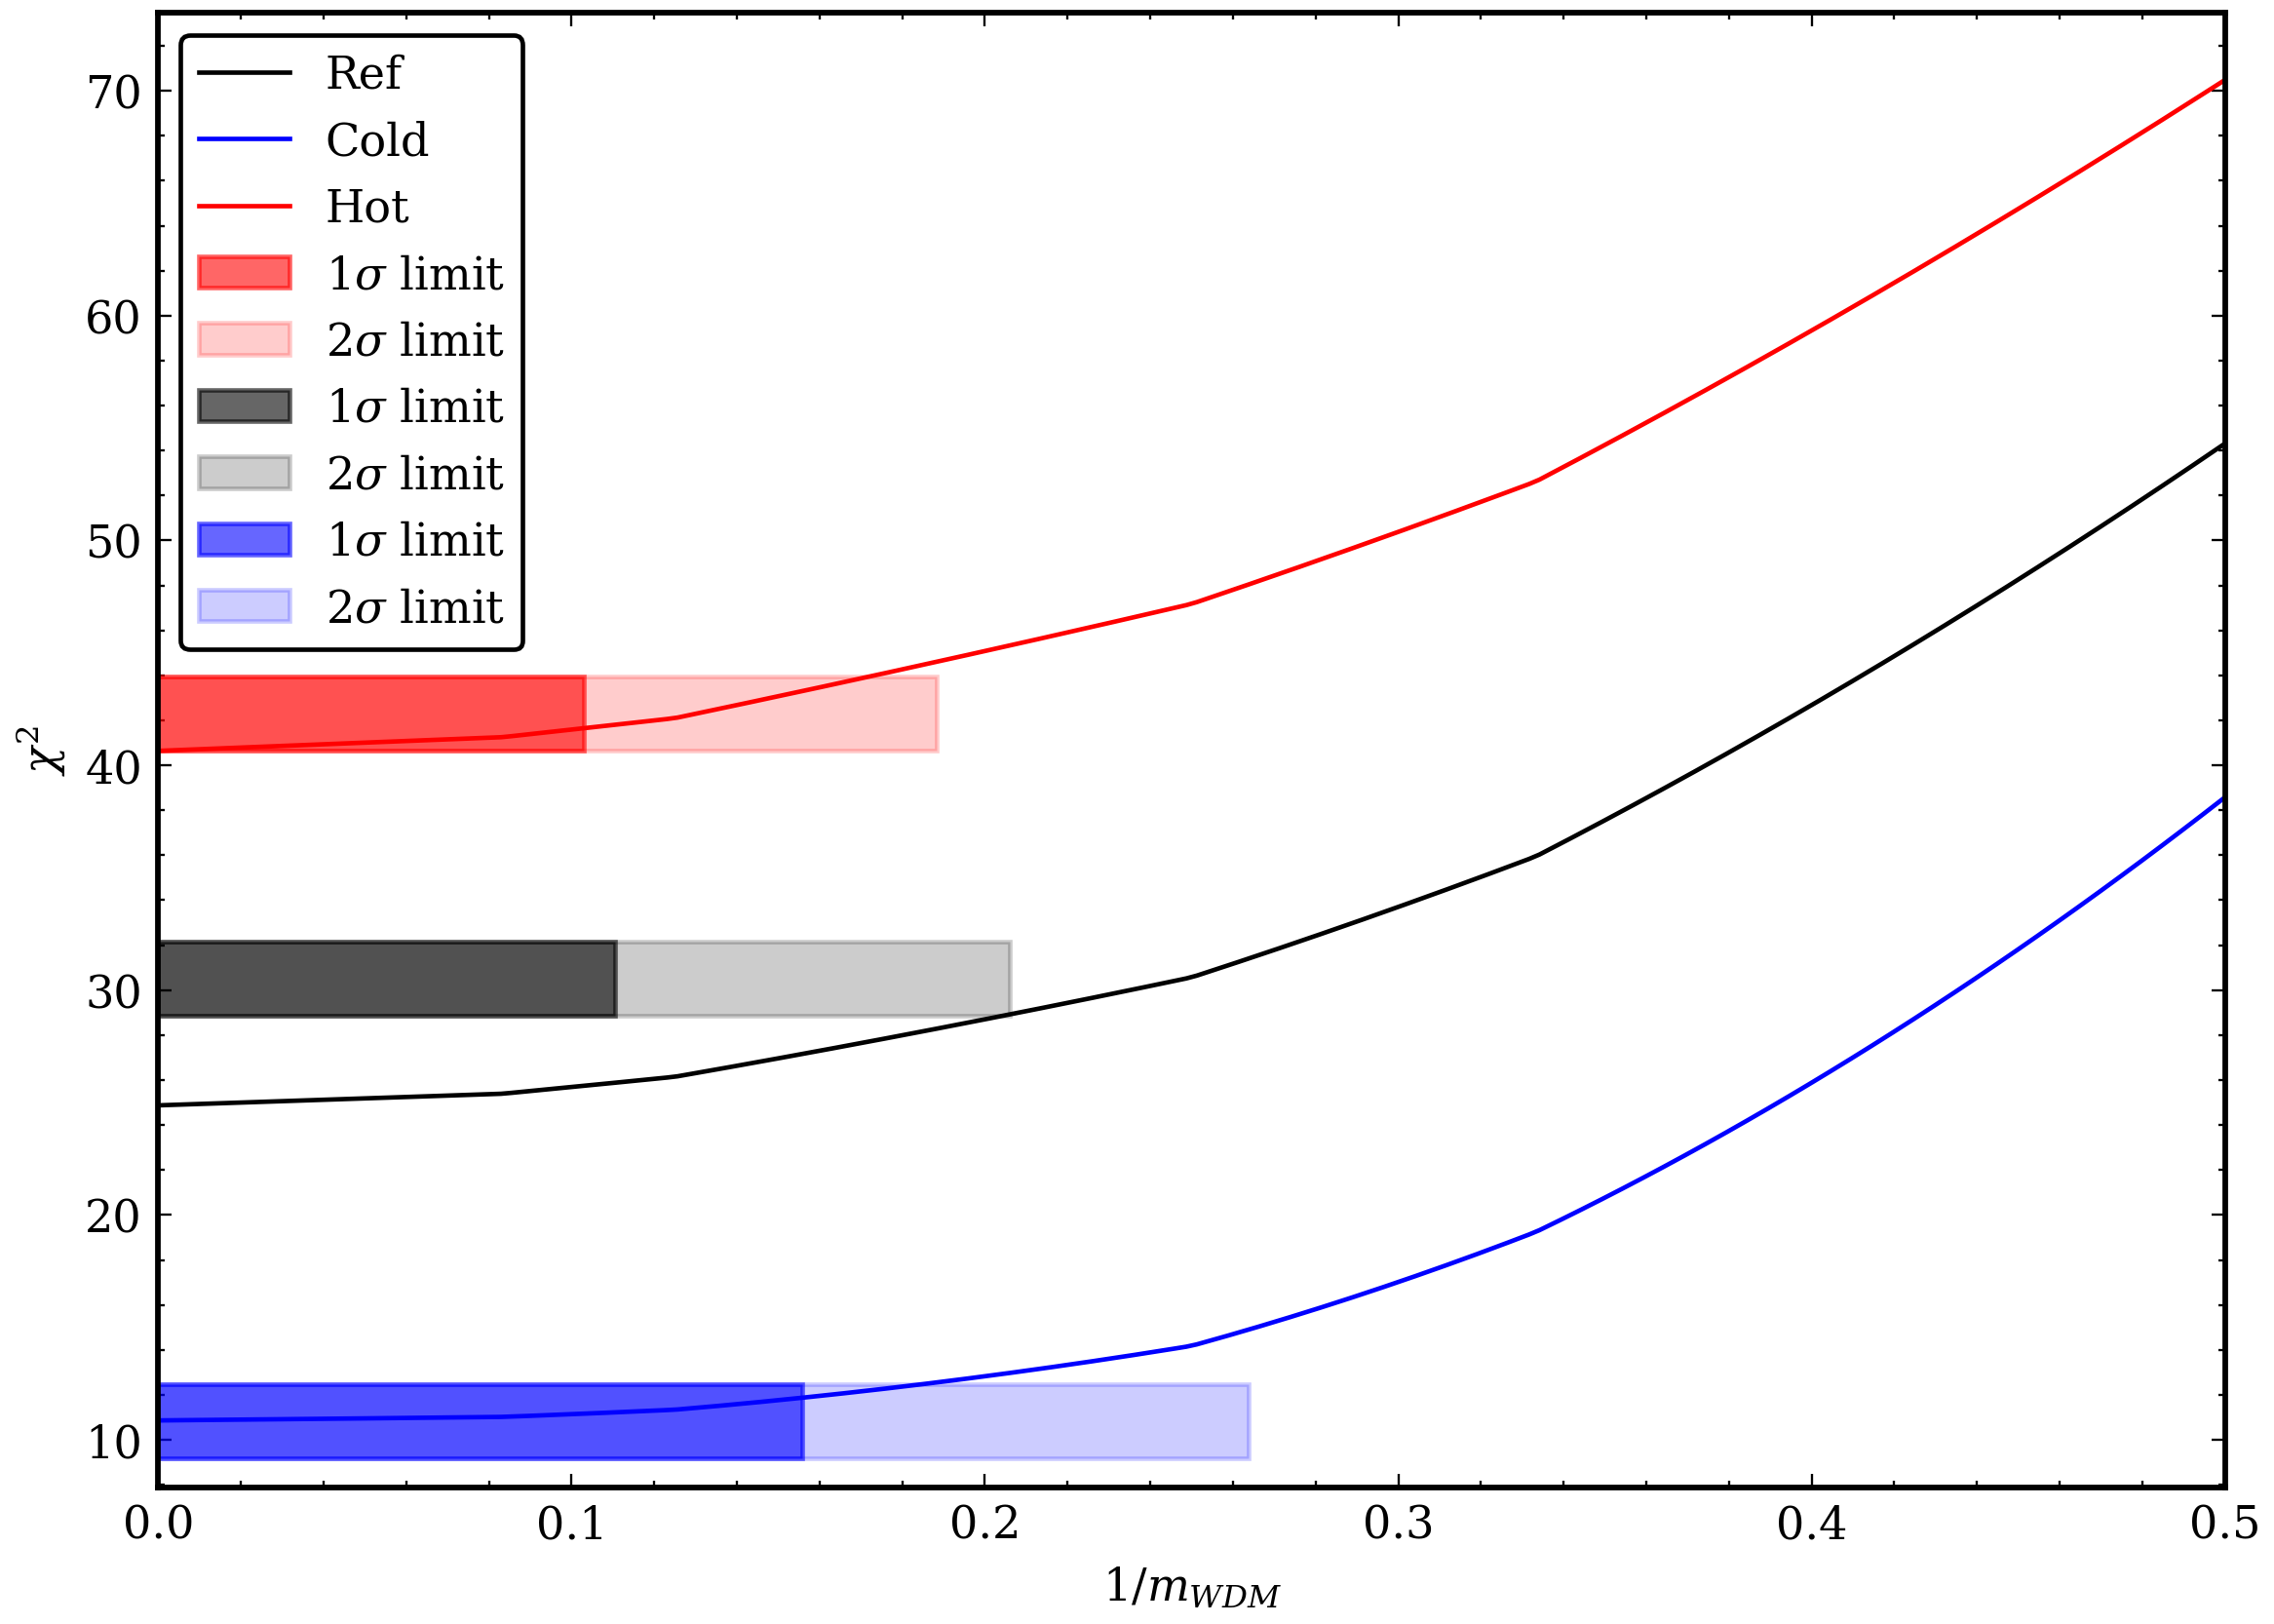
\includegraphics[width=1\textwidth]{img/ML/squad_chi.png}
    
    \end{subfigure}
    \hfill
    \begin{subfigure}[b]{0.45\textwidth}
        \centering
        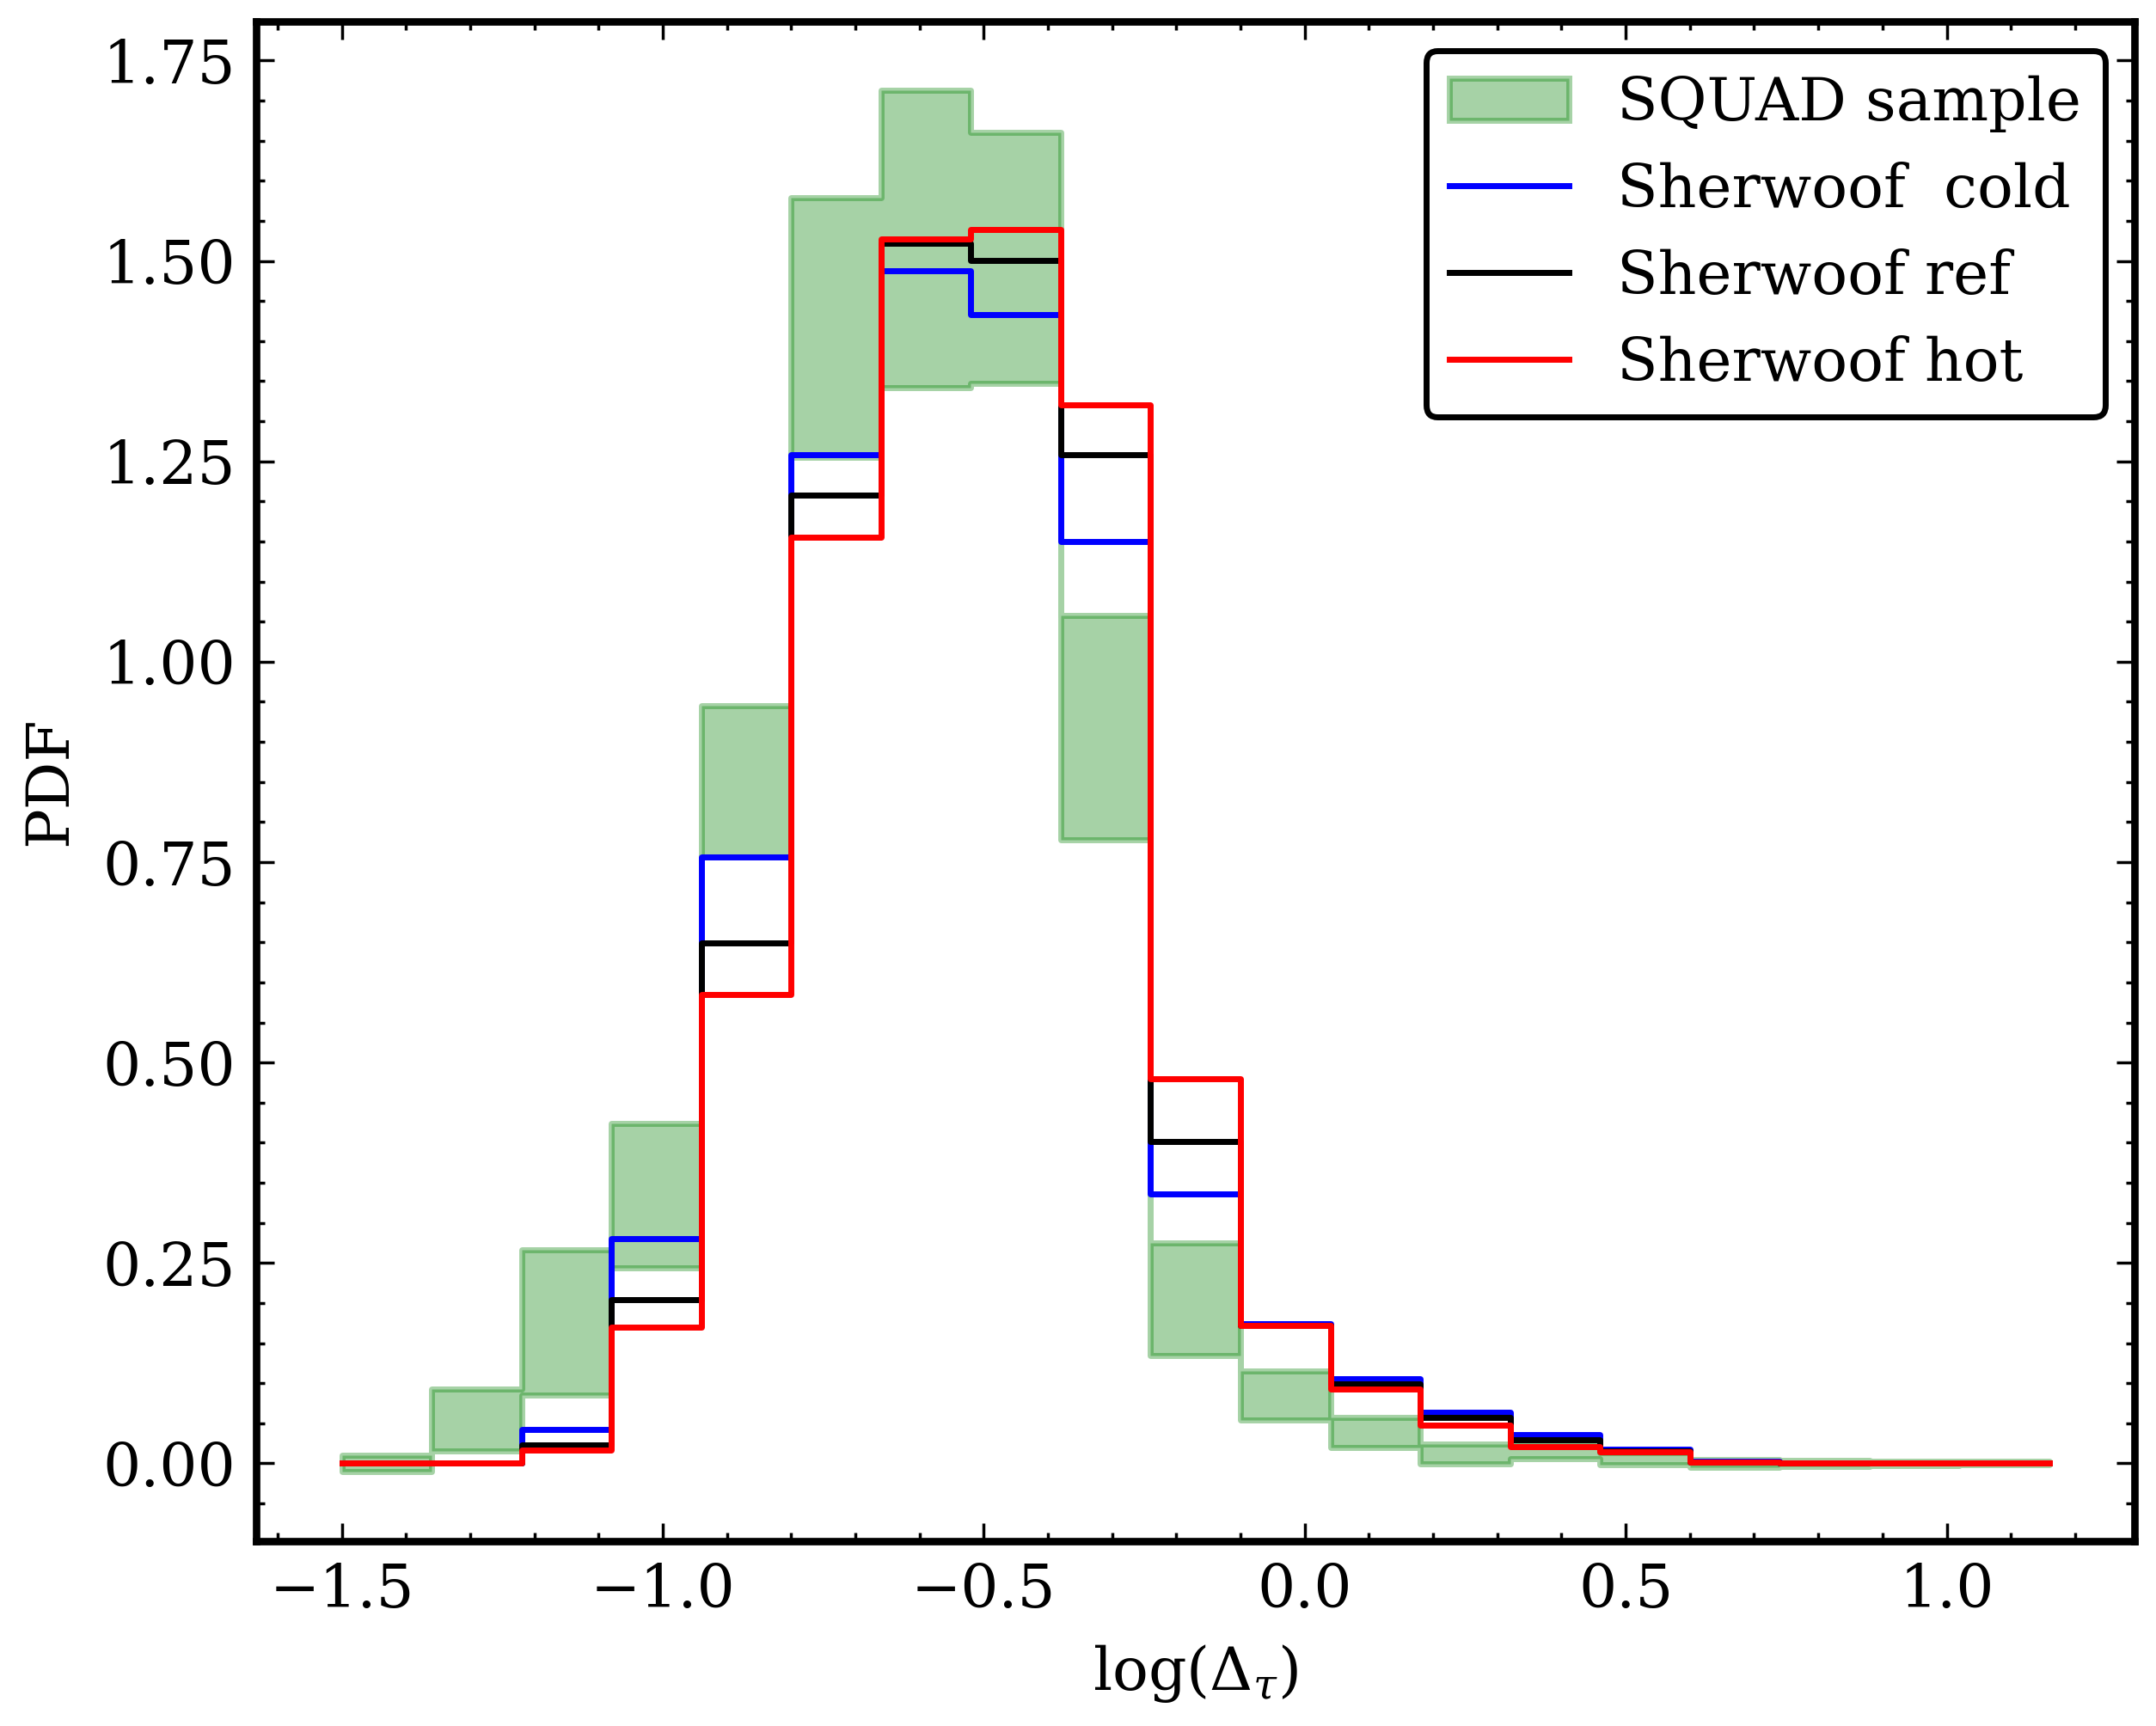
\includegraphics[width=1\textwidth]{img/ML/squad_fit_pdf.png}     
    \end{subfigure}
        \caption{In the left panel, we show all 3 $\chi^2$ curves as a function of the WDM mass, together with the $1,2\sigma$ confidence regions. The right panel shows the recovered $\Delta_\tau$ PDF from the SQUAD DR1 sample with the symmetric uncertainty envelop, together with the best-fit model, corresponding to the CDM cold \texttt{SHERWOOD THERMAL} model.
        }
        \label{fig: squad chi pdf}
\end{figure}










\section{WDM constraints from GHOST observed spectrum}\label{sec:inference ghost}
We also consider a Lyman-$\alpha$ skewer obtained from the GHOST instrument, which corresponds to the ultra-luminous quasar J0306+1853 \cite{Wang_2015} with emission redshift $z=5.363$. For this spectrum, we have a continuum reconstruction in the range $[971, 1210]$ \textup{~\AA} in the emission rest frame, with an average signal-to-noise ratio of $\mathrm{SNR}\approx 150$. We extract skewers of length 20h$^{-1}$cMpc and consider them independent in order to run the neural network predictions. In total, we obtained 13 such sightlines and discarded the range $\approx [1120,1162]$ \textup{~\AA} that contains a DLA.


\begin{figure}
    \centering
    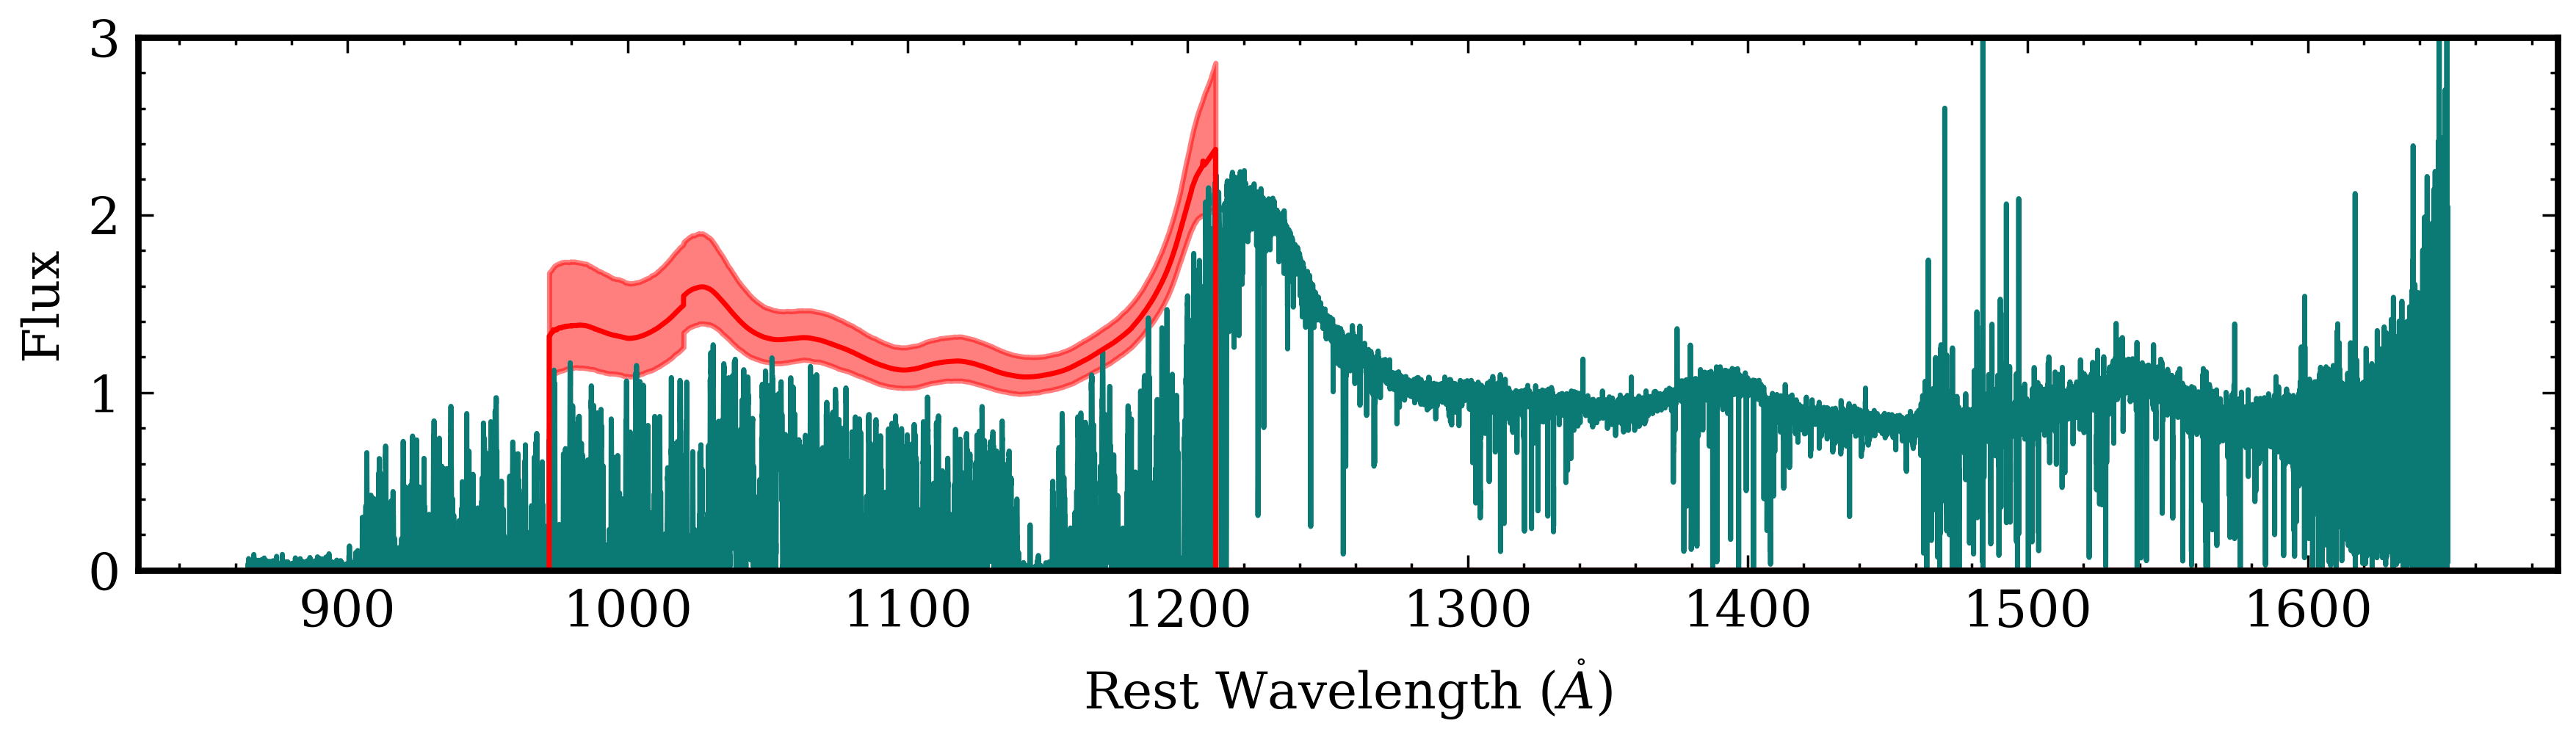
\includegraphics[width=0.7\linewidth]{img/ML/ghost_spectrum.png}
    \caption{THE GHOST spectrum for J0306+1853 \cite{Wang_2015}. The red curve shows the reconstructed continuum together with $1\sigma$ uncertainties, obtained with a PCA technique based on the spectrum to the right side of the Lyman-$\alpha$ line. Observe the DLA at $\sim 1150$ \textup{~\AA}, which we mask when analysing the Lyman-$\alpha$ forest. }
    \label{fig: ghost spectrum}
\end{figure}



Figure \ref{fig: ghost rec} shows an example 20h$^{-1}$cMpc portion of the spectrum together with the recovered density field. We split the original spectrum into 13 such skewers of the same length as the ones of the \texttt{Sherwood} dataset, and consider them independent.

We apply our WDM inference pipeline to the 13 segments of the J0306+1853 spectrum. The $\chi^2$ is minimised for the CDM model within each thermal history, and the best-fit thermal model is the \texttt{SHERWOOD THERMAL} CDM reference run. The corresponding $2\sigma$ constraint on the WDM mass is $m_{\mathrm{WDM}} \gtrsim 4.4$ KeV at $2\sigma$ confidence.




\begin{figure}[h!]
    \centering
    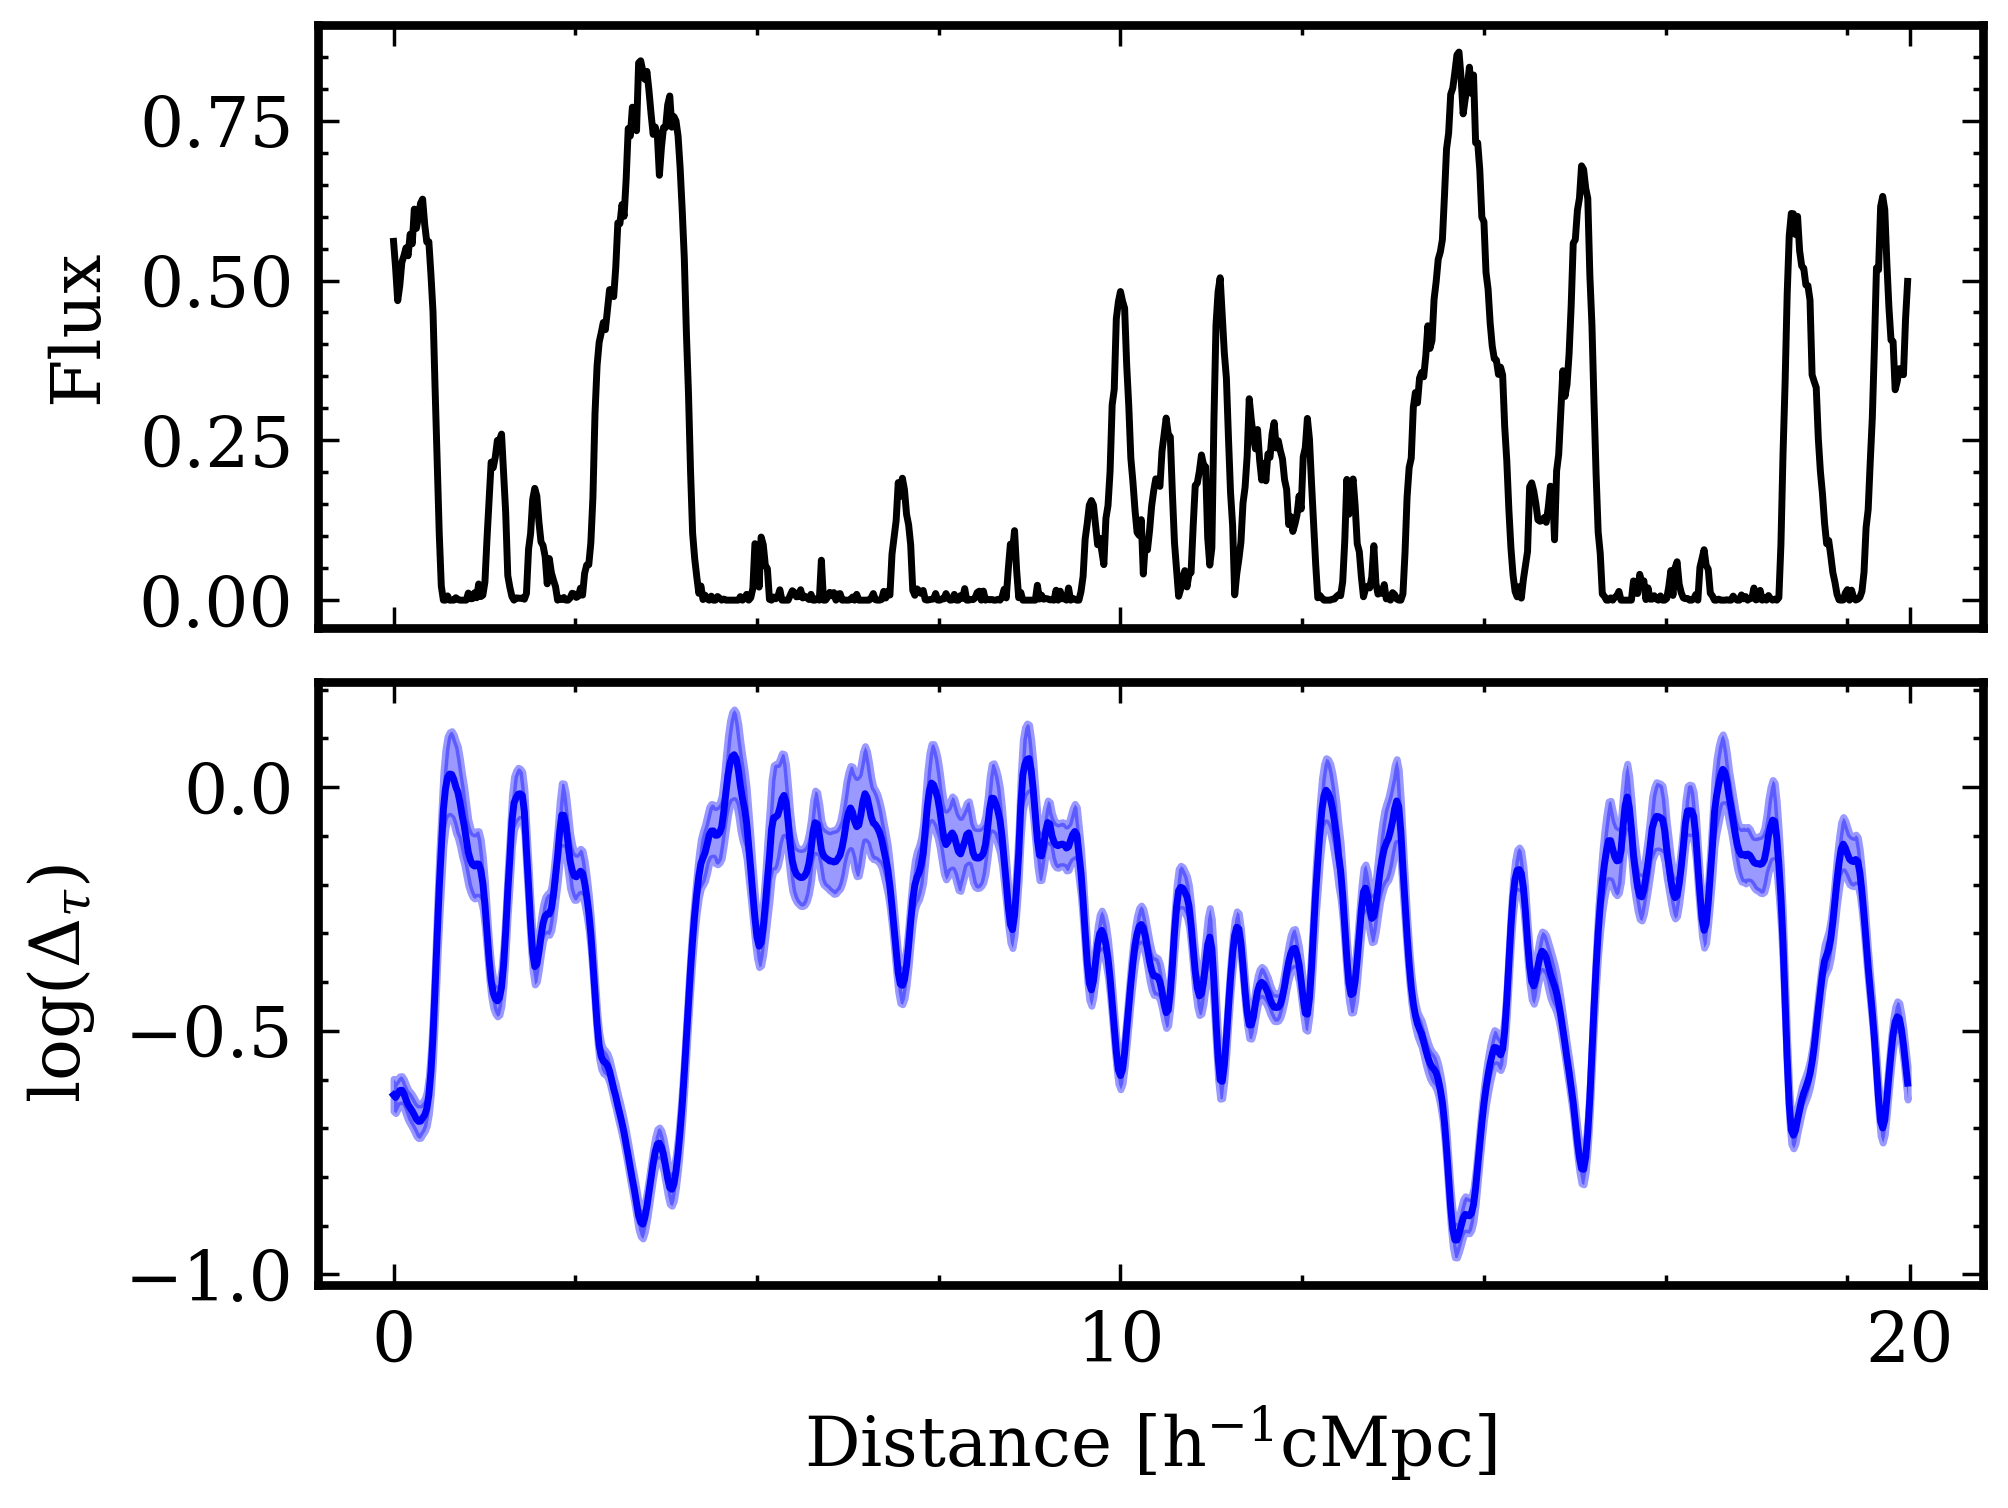
\includegraphics[width=7.5cm]{img/ML/ghost_recovered.png}
    \caption{An example 20h$^{-1}$cMpc portion of the J0306+1853 spectrum together with the recovered density field. We split the original spectrum into 13 such skewers of the same length as the ones of the \texttt{SHERWOOD THERMAL} dataset, and consider them independent.}
    \label{fig: ghost rec}
\end{figure}


In Table \ref{tab: summary constraints} we list the current state-of-the-art $2\sigma$ lower bounds on $m_{\mathrm{WDM}}$ thermal relics constraints in the literature obtained from the Lyman-$\alpha$ power spectrum. The previous efforts are based on a Bayesian inference framework to compare the observed power spectrum with the one obtained from simulated data. In contrast, in our work, we do the inference directly on the non-observable density field level. The resulting bounds produced in our work are comparable to previous efforts but with the advantage of requiring substantially less observational data. For reference, in \cite{sherwood_wdm}, the constraints are obtained from 15 spectra measured along 327h$^{-1}$cMpc,  while our GHOST data consists of 13  20h$^{-1}$cMpc skewers. The tightening of the constraint from the SQUAD DR1 sample to the GHOST sample is also expected since the latter is a larger sample with lower noise.
\begin{table}[h!]
    \caption[]{List of  current state-of-the-art $2\sigma$ lower bounds on $m_{\mathrm{WDM}}$ thermal relics constraints in the literature obtained from the Lyman-$\alpha$ power spectrum. We compare them to the results of this work, obtained doing inference directly at the density field level recovered by our Bayesian neural network. }
       \label{tab: summary constraints}
   $$ 
       \begin{array}{p{0.4\linewidth}c}
          \hline
          \noalign{\smallskip}
          Source &  2\sigma\ m_{\mathrm{WDM}} \mathrm{{\ lower \ bound\ [KeV]}}  \\ 
          \noalign{\smallskip}
          \hline
          \noalign{\smallskip}
          Ir\v{s}i\v{c} et al. (2024) \cite{sherwood_wdm} & 4.1      \\
          Villasenor et al. (2023) \cite{Villasenor_2023} & 3.1      \\
          \noalign{\smallskip}
          \hline
          \noalign{\smallskip}
          This work (SQUAD DR1 sample)  & 3.8   \\
          This work (GHOST spectrum)  & 4.4        \\

          \noalign{\smallskip}
          \hline
       \end{array}
   $$ 
 \end{table}















\section{Comparison of the inference pipeline against Information Maximising Neural Networks}


The inference pipeline presented so far in this section is based on a simple $\chi^2$ fit of the $\Delta_\tau$ recovered PDFs from our fiducial NN model. This pipeline rellies on a series of contingent choices, most notably the use of the density PDFs as the summary statistics of the fields. In this section, we explore, in an agnostic way, the possiblity of using other summaries different from the $\Delta_\tau$ PDFs to perform the inference (note that other summaries such as the density power spectrum, curvature,... could potentially be used). More concretely, we will introduce Information Maximising Neural Networks (IMNNs) and use them to perform the inference within a Bayesian framework. We then compare the results of this procedure with the inerence pipeline discussed in section \ref{sec: inference pipeline}.

\subsection{Information Maximising Neural Networks}
Information Maximising Neural Networks aim at obtaining optimal summaries of data \cite{Charnock_2018}. Neural networks are used to parametrise these summaries in an agnostic way by maximising the information of the summaries with respect to the model parameters of interest.

Consider a data-generating procedure depending on some model parameters $\theta$, generating data realization $d_i(\theta)$ where $i$ labels a realization or initial seed of the simulation. We want to obtain a function $f \colon d \mapsto x$ that maps each simulation to a summary vector of the same size as $\theta$. This is, essentially, a compression algorithm. IMNNs work by transforming the original likelihood of the data, which is a priori not known, into the gaussian form

\begin{equation}
    -2\ln\mathcal{L}\left(x|\theta\right)=\left(x-\mu\left(\theta\right)\right)^TC^{-1}\left(x-\mu\left(\theta\right)\right),
\end{equation}

where $C$ is the covariance matrix of the calculated summaries with a set of $n_s$ simulations, and $\mu$ the summary mean depending on the model parameters. The information of the observed summaries with respect to $\theta$ is then the Fisher information matrix \cite{ly2017tutorialfisherinformation}:

\begin{equation}\label{eq:Fisher information}
    F_{\alpha \beta} =-\operatorname{E}\bigg[\frac{\partial^2}{\partial\theta_\alpha\partial\theta_\beta}\log \mathcal{L}(x;\theta)\bigg|\theta\bigg]= \frac{\partial \mu}{\partial \theta_\alpha}C^{-1} \frac{\partial \mu}{\partial \theta_\beta},
\end{equation}
whose determinant we note as $|F|$. 
The goal is to obtain summaries that maximise the Fisher information while mainting a minimum covariance condition to generate independent summaries. The summaries produced by the network can then be used to perform inference on them. Since the Fisher information is a quantity that depends on the model paramters $\theta$, the quantity in Equation \ref{eq:Fisher information} needs to be evaluated at some fiducial model parameters in order to obtain a numerical result.

IMNNs have been succesfully leveraged in the IGM community. Recent papers have explored the possibility of using them to perform IGM thermal paramter inference from Lyman-$\alpha$ skewers, see \cite{maitra2024parameterestimationlyalphaforest} for instance, where authors find IMNNs to yield tighter and more robust constraints than classical Markov Chain Monte Carlo approaches. Despite these promising results, many challenges arise when using IMNNs on real data, primarly related to the correct identification and interpretation of model parameters.

\subsection{IMNN training and non-linear summaries}
In this section we consider a simple MLP architecture with linear layers followed by PReLU($\alpha$) activation functions and a dropout layer that randomly (with probability $p$) sets to 0 the any layer weight during each epoch to prevent over-fitting. The network takes as input a simulated data vector $d$ and prodcued a summary vector $x$ of the same size and the parameter vector $\theta$. We use the Adam optimiser to maximise |F| by minimising the following loss function

\begin{equation}\label{eq:IMNN loss}
    \mathcal{L}_{IMNN} = - \log(|F|) + \lambda \frac{\mathcal{N}}{\mathcal{N}+\exp(-\mathcal{N})} \mathcal{N},
\end{equation}
where $\mathcal{N}=||C-I||+|C^{-1}-I|||$ measure the deviation from independt summaries and $\lambda$ is a coupling constant. In Equation \ref{eq:IMNN loss}, the second term sets a scale for the Fisher information by producing summaries whose covariance approaches the identity matrix. Once this is achieved, the term containing the exponential factor vanishes and the network will maximise $|F|$. Note that there is not a unique set of potential optimal sumamries. In fact, any bijective function of a sufficient statistic for a certian likelihood is also a sufficient statistic.

For each paramter update in the training procedure, we generate a batch of data at the fidicual parameters $\theta_f$. The derivatives in Equation \ref{eq:Fisher information} are numerically approximated with finite differences by running simulations at parameters $\theta_f \pm \Delta \theta_\alpha$, where $\Delta \theta_\alpha$ are a small parameter variation, and then calcualting

\begin{equation}
    \frac{\partial x}{\partial \theta_\alpha}=\frac{x(d(\theta_f + \Delta \theta_\alpha))-x(d(\theta_f - \Delta \theta_\alpha))}{2 \Delta \theta_\alpha}.
\end{equation}
We then calculate $C$, the covariance of the summaries at fiducal paramters, and use it to compute the Fisher information in Equation \ref{eq:Fisher information} and the loss function in Equation \ref{eq:IMNN loss}. Note that, since the covariance matrix and the derivative in the Fisher information matrix are computed at the data summaries, they implicitely depend on the NN parameters.

\subsection{Summarising a Gaussian signal}\label{sec:IMNN normal}
We implement IMNNs using Pytorch\footnote{\url{https://pytorch.org}}, a deep-learning Python framework. We test the implementation first by exploring its behavior on a toy model, where we generate ramdon samples from a Gaussian distribtion $\mathcal{N}(\mu, \sigma)$. The sufficient statistic for the model parameters $\theta=(\mu,\sigma)$ are, in this case, the sample mean and standard deviation:

\begin{equation}
    \hat{\mu}=\frac{1}{n_d}\sum d_i \hspace{1cm} \hat{\sigma}^2 = \frac{1}{n_d-1}\sum (d_i -\hat{\mu})^2.
\end{equation}
Note that the statistic for $\sigma$ is non-linear.
For this example, we select fiducial parameters $\theta_f=(\mu=0, \sigma=1)$ and $\Delta \theta=(0.1 , 0.1)$ and generate random fields with 100 pixels. In total, 5000 fields are generated for each parameter set, including a validation dataset. Note that testing the network performance in the validation dataset is crucial in performing early-stopping during the training process. Indeed, since the training dataset is limited, it will contain spurious correlations that the network will use to infer a higher information than expected. By stopping the training when the network information on the validation set saturates, we can avoid this problem. We use a simple architecture, with layers $[128,128,128,2]$, learning rate of $0.001$, dropout rate of $p=0.5$, and batch size of $500$. Observe the training evolution in Figure \ref{fig:IMNN training normal test}, where we show $|F|$ and $||C-I ||+||C+I||$ as a function of the epoch for the training and validation sets. As can be seen, the validation information quickly saturates in $\sim 100$ epochs, and then slowly decreases as the network over-fits.

\begin{figure}
    \centering
    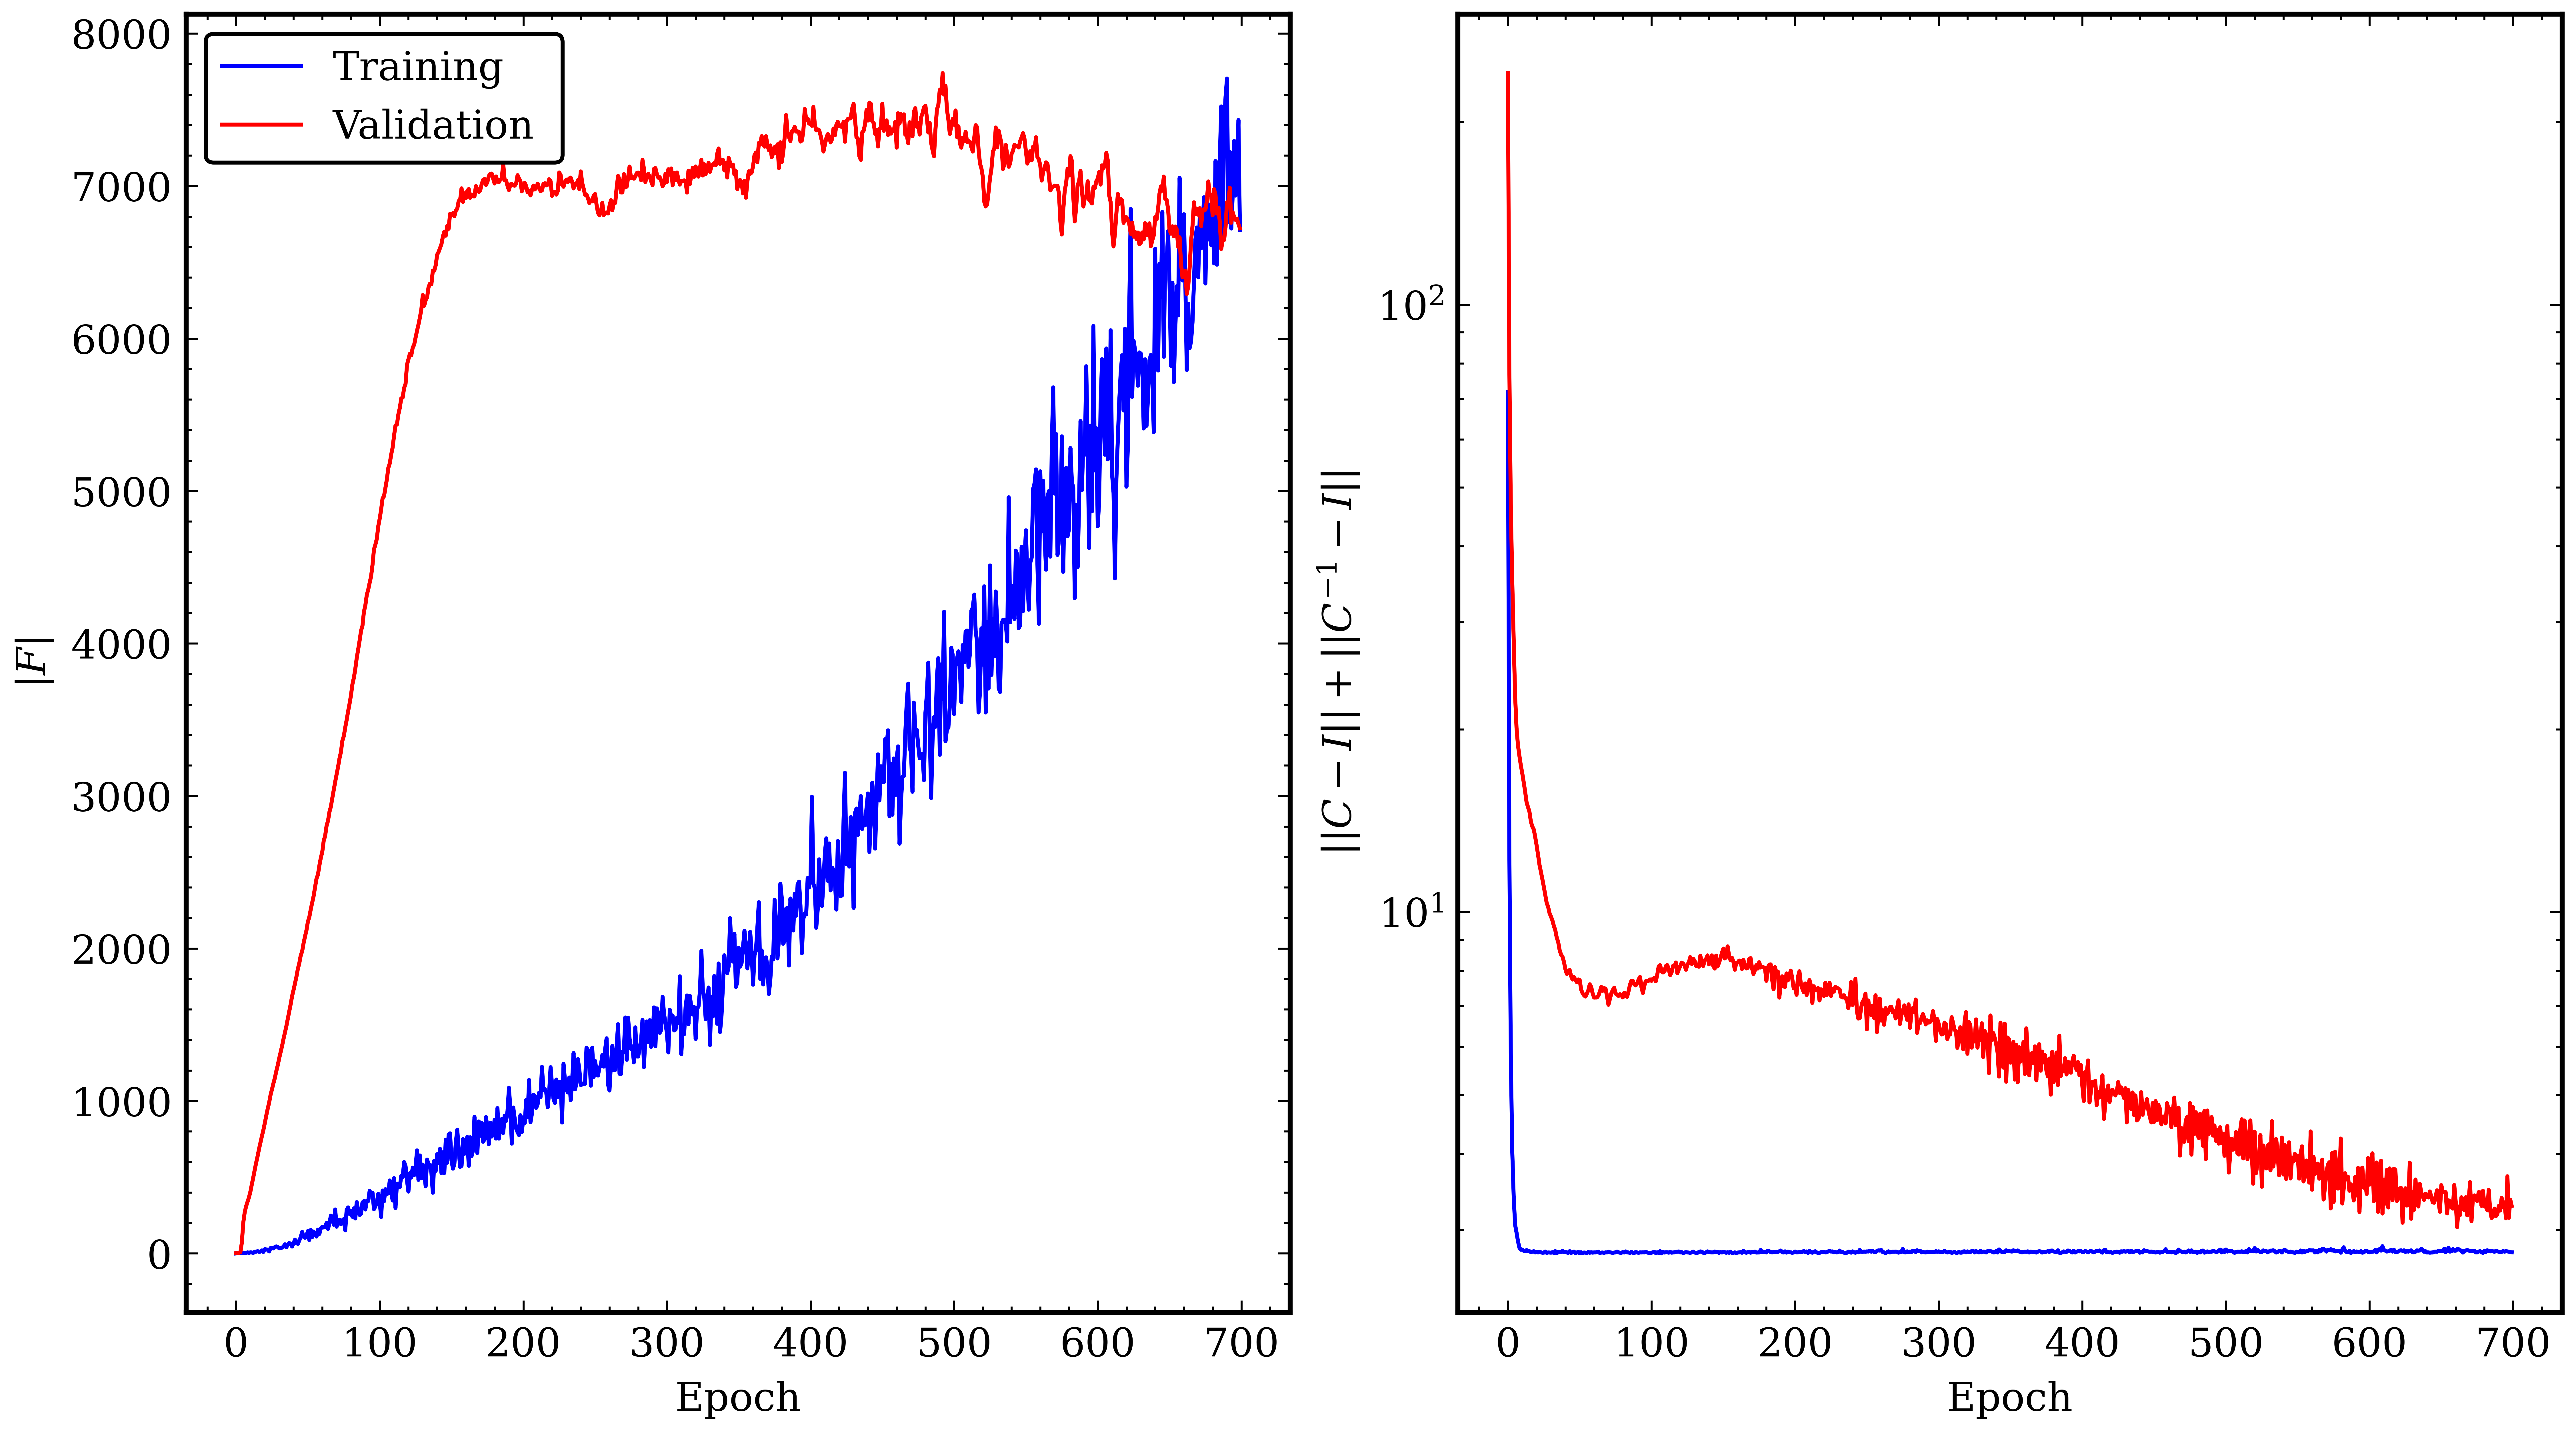
\includegraphics[width=0.95\linewidth]{img/ML/normal_plot_training.png}
    \caption{$|F|$ and $||C-I ||+||C+I||$ as a function of the epoch for the training and validation sets during the training of the IMNN on a normal field. The goal is to find summaries to optimally extract information about the mean and variance of the field.}
    \label{fig:IMNN training normal test}
\end{figure}

To better interpret the network output and to understand its behavior, we generate samples of the same size with the zero mean but a standar deviation randomly sampled from $(0,12)$. We then compute the exact statistic (the sample standar deviation) and plot it against the second IMNN sumamry output. The result is Figure \ref{fig:IMNN normal std}. Observe that the exact statistic in the $x$-axis is highly correlated to the network summary in the $y$-axis. Since the relation between the two quantities is clearly bijective, the model has succesfully learnt to extract all the possible information for the field covariance. The natural scatter is due to having a simple NN model.

\begin{figure}
    \centering
    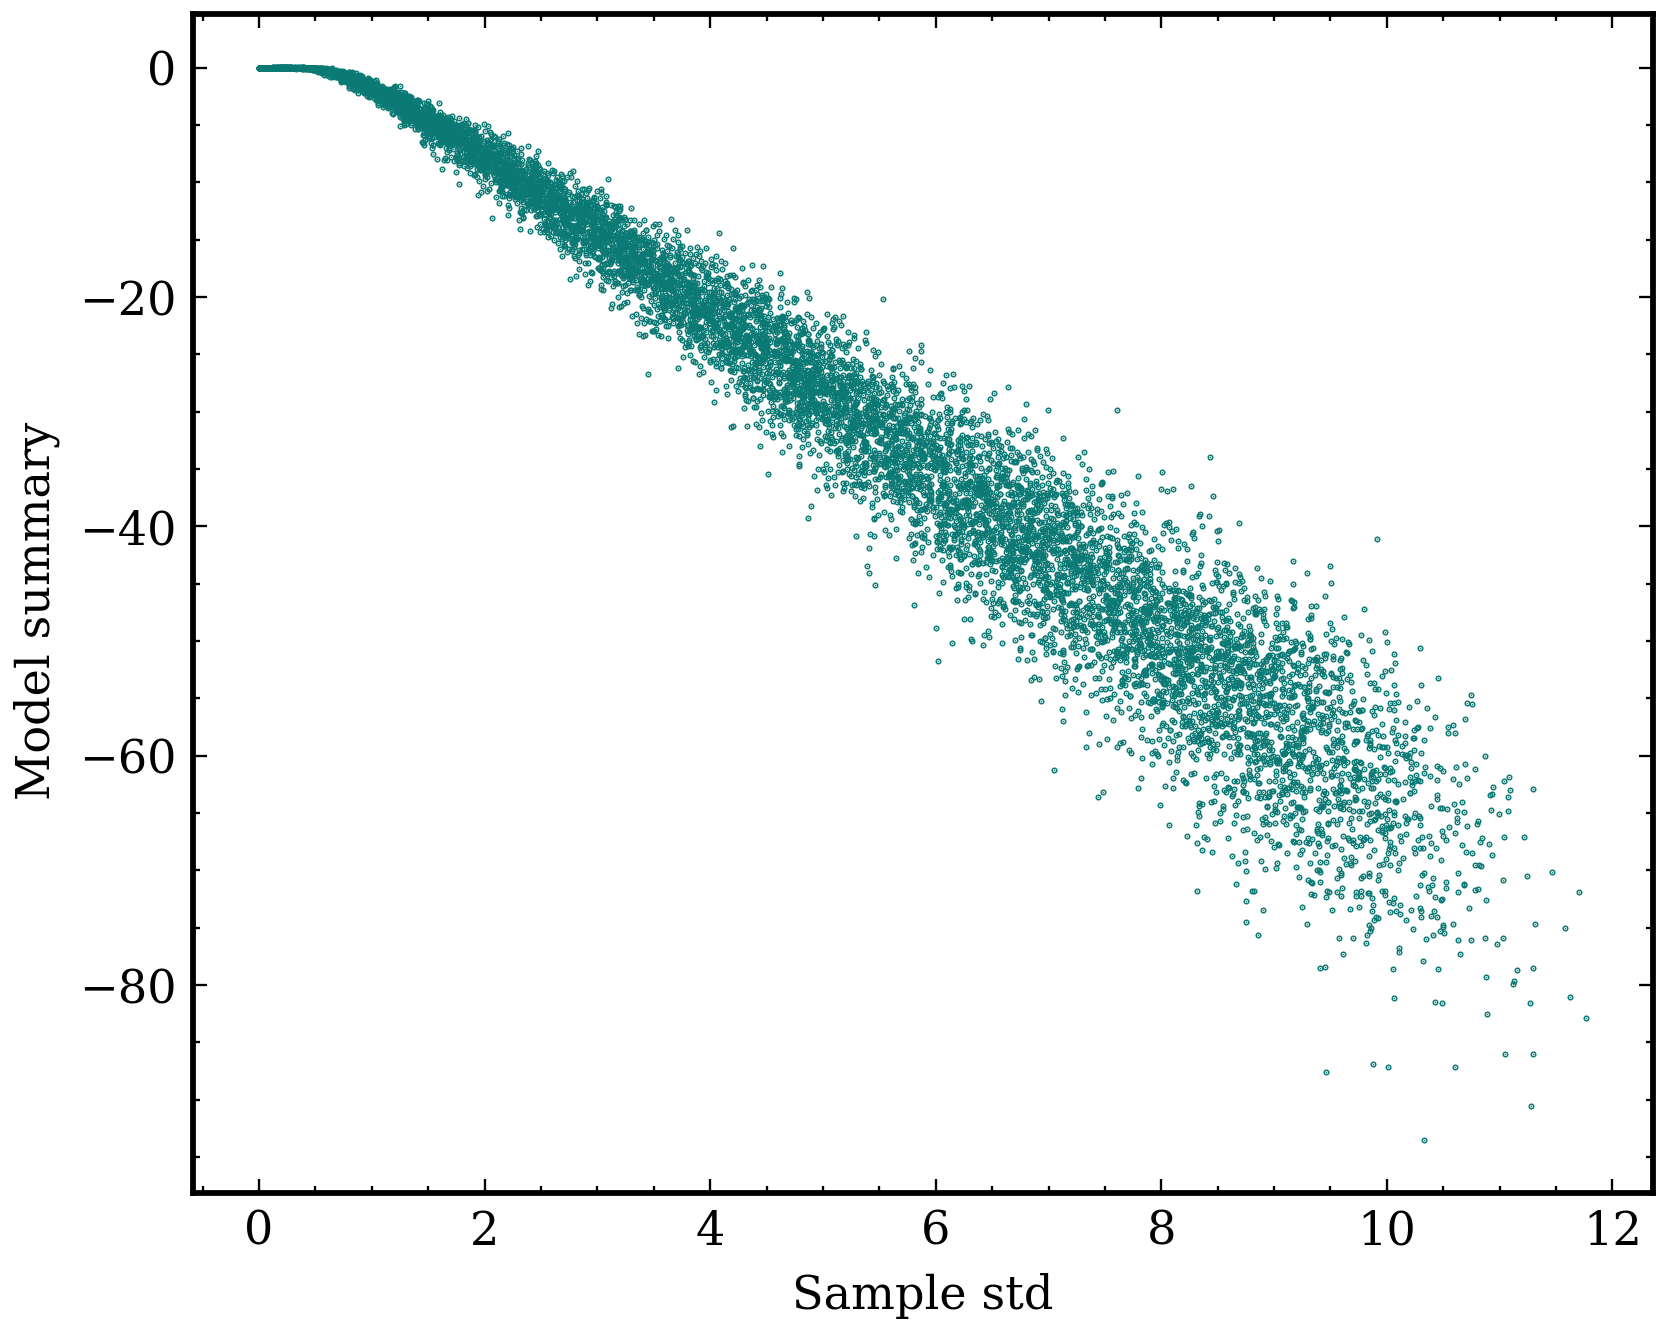
\includegraphics[width=0.75\linewidth]{img/ML/std_vs_model.png}
    \caption{The IMNN summary plotted agains the exact sufficient statistic for the standard deviation using multiple samples with $\sigma \in (0,12)$.}
    \label{fig:IMNN normal std}
\end{figure}
Note that the network has not seen any normal field with such variances $\sigma \in (0,12)$ during training, yet it is able to extract the correct summary. This is of crucial importance, since it means that we could use the IMNN summaries to do inference on a field with parameter values slighly different from the fiducial ones used during training.


To conclude the exploration of this toy model, we use the network to perform Bayesian inference. We implement a simple Approximate Bayesian Computation (ABC) \cite{review_ABC} algorithm that obtains approximate posterior samples from a given set of prior samples and observed data. As the observed data, we take 50 Gaussian fields simulated at fiducial parameter $(\mu=0, \sigma=1)$ values. As priors, we take 5000 samples from a non-informative uniform distribution in $(-5, 5)$ for $\mu$ and $(0, 10)$ for $\sigma$. The ABC rejection algorithm is described in Algorithm \ref{alg:ABC}.


\begin{algorithm}
    \caption{Approximate Bayesian Computation Rejection Algorithm}\label{alg:ABC}
    \begin{algorithmic}[1]
    \State \textbf{Input:} Observed data $\mathbf{y}$, threshold $\epsilon$, number of simulations $N$, prior distribution $\pi(\theta)$
    \State \textbf{Output:} Accepted parameter values $\{\theta_i\}_{i=1}^M$
    
    \State Initialize $M \gets 0$
    \For{$i = 1$ to $N$}
        \State Sample $\theta^*$ from the prior distribution $\pi(\theta)$
        \State Simulate data $\mathbf{y}^*$ from the model using $\theta^*$
        \If{$d(\mathbf{y}, \mathbf{y}^*) \leq \epsilon$}
            \State Accept $\theta^*$: $\theta_{M+1} \gets \theta^*$
            \State Increment $M \gets M + 1$
        \EndIf
    \EndFor
    
    \State \textbf{return} $\{\theta_i\}_{i=1}^M$
    \end{algorithmic}
    \end{algorithm}
In Figure \ref{fig:IMNN normal posterior} we show the posterior samples and Gaussian Kernel Density Estimation (KDE) for the distributions of $\mu$ and $\sigma$. The dashed vertical lines show the true parameter values. As expected, and even with a non-informative prior, the IMNN summary contain sufficient information to produce tight posterior around the true model parameters. Note that the posterior scatter on the non-linear summary $\sigma$ is larger than on the linear summary $\mu$.

\begin{figure}
    \centering
    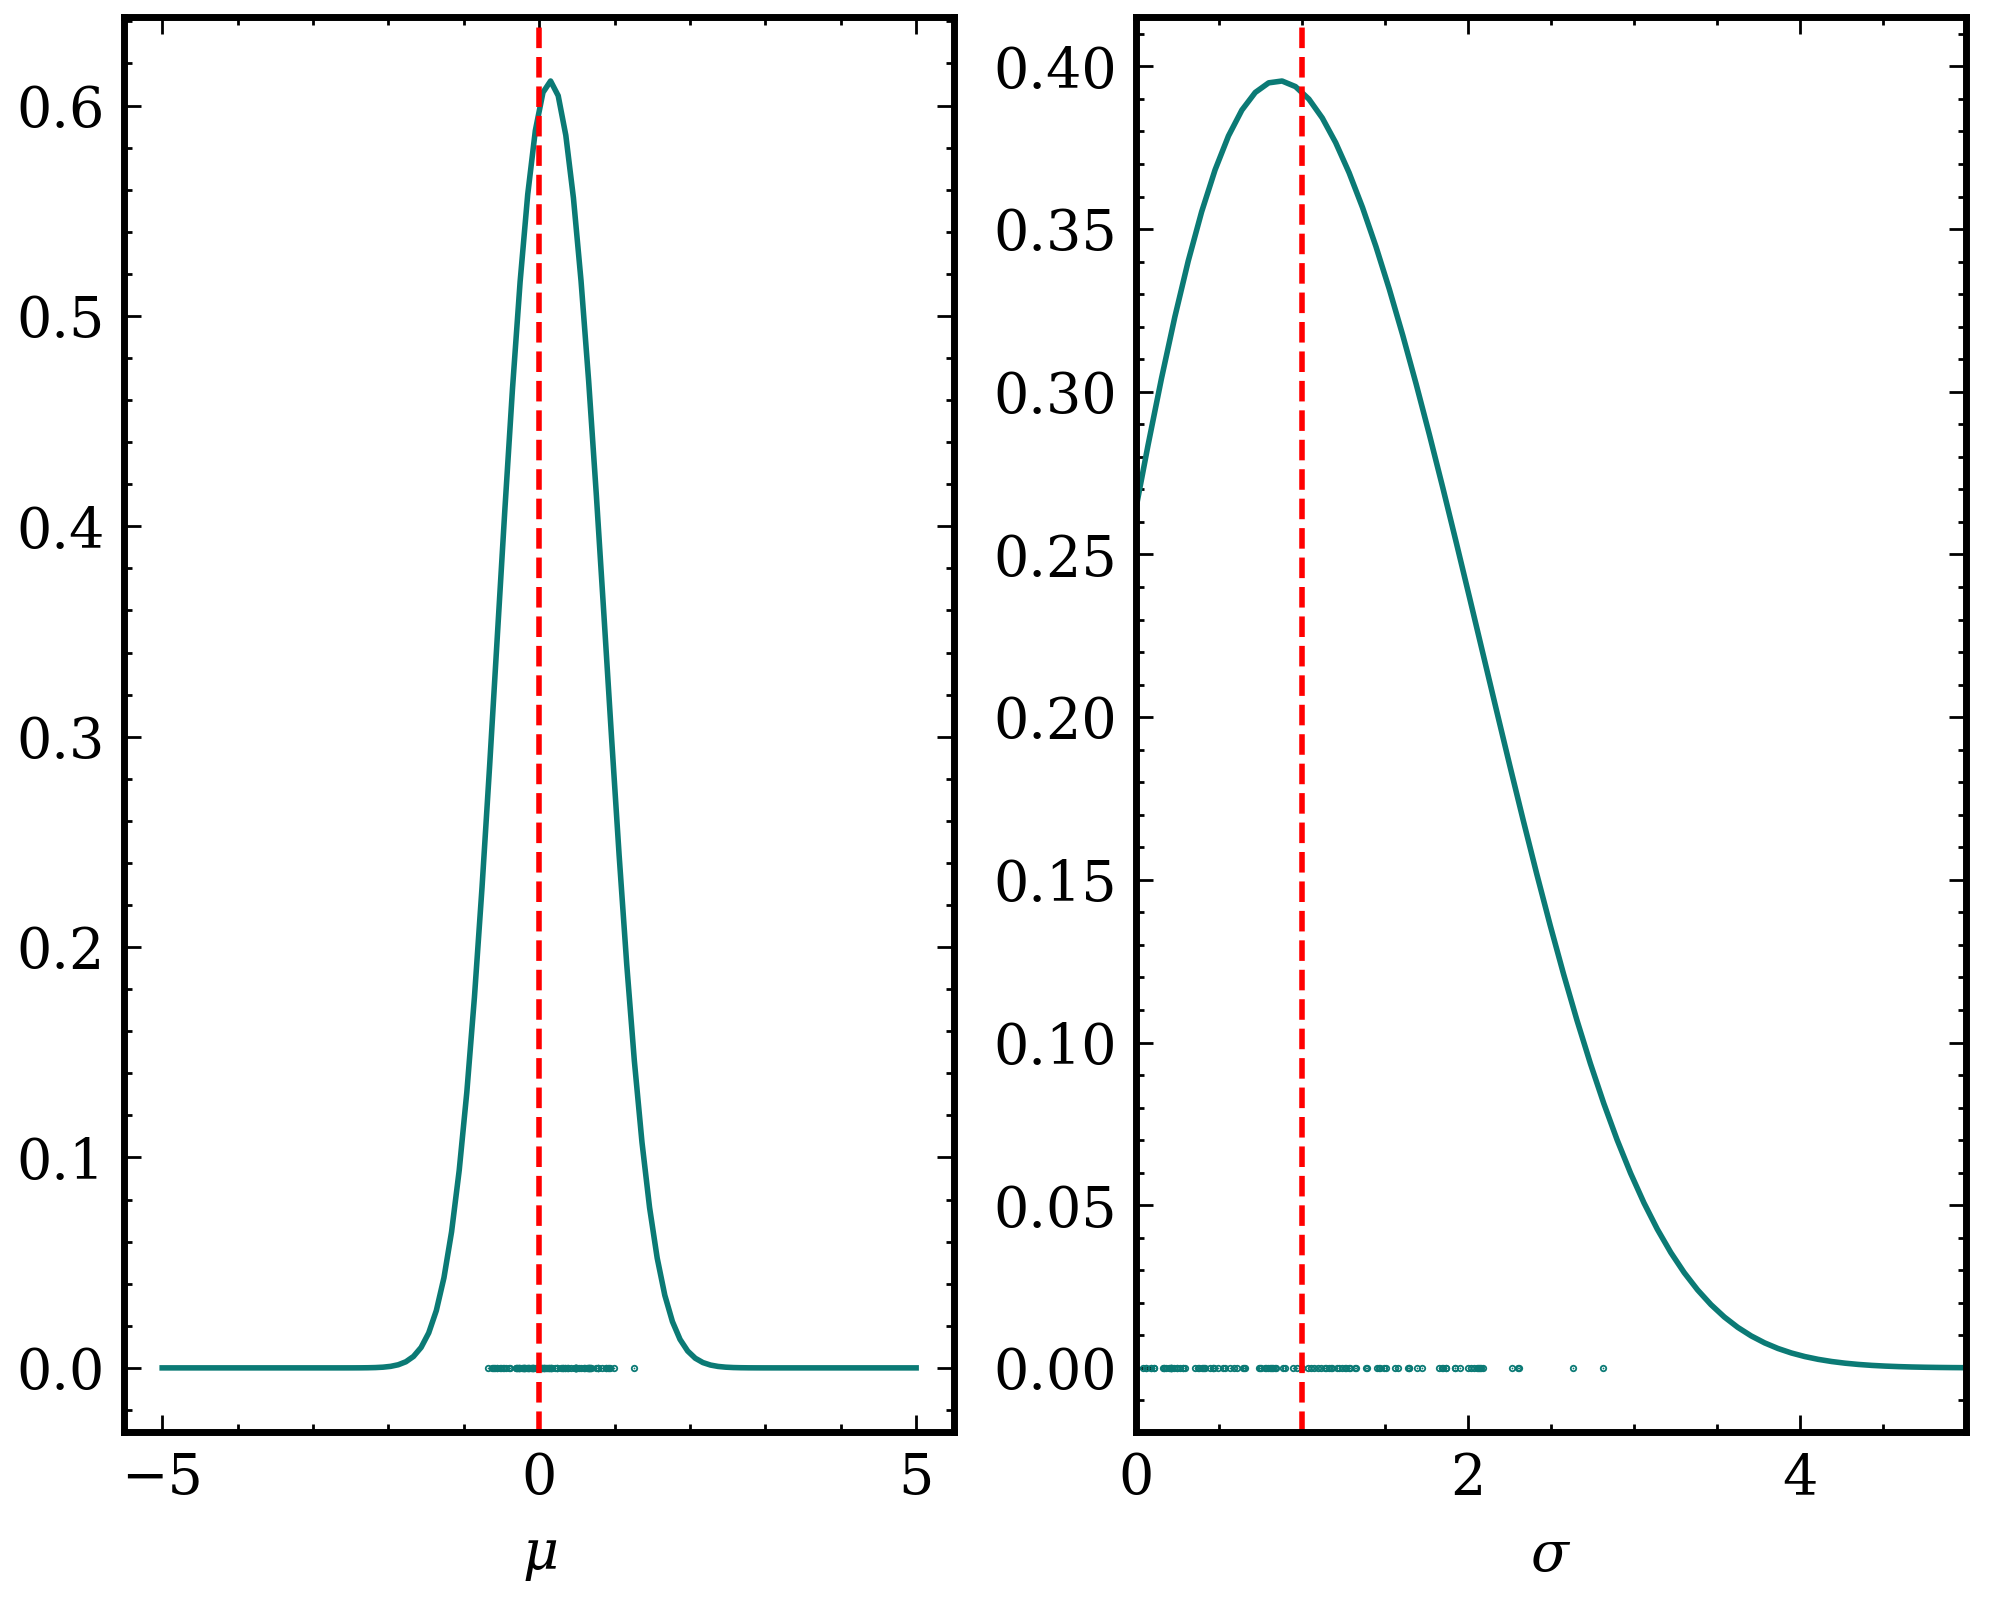
\includegraphics[width=0.75\linewidth]{img/ML/ABC_posteriors_normal.png}
    \caption{Posterior samples and KDE for the ABC rejection algorithm applied to the normal toy model, where we infer the mean and variance of a Gaussian field with flat priors and the summaries output of a IMNN. The dashed vertical lines show the true parameter values.}
    \label{fig:IMNN normal posterior}
\end{figure}






\subsection{IMNN inference results on WDM masses}\label{sec:IMNN}
We can now deploy a simple IMNN as an alternative way of constraining WDM models. We follow section \ref{sec:IMNN normal} and consider a similar architecture but now with 4 dense layers of size $[512, 512, 256, 2]$. As input to the NN, we consider Lyman-$\alpha$ flux skewers. Since in flux space the skewers has many simulation-specific and prominnent features that can be picked-up by a NN, we work in Fourier space. More precisely, the input to the network are 
\begin{equation}
    \sqrt{k} |\delta_F (k)|,
\end{equation}
where $\delta_F$ is the flux contrast of the skewer.
We use the \texttt{SHERWOOD} simulation suite with varied WDM mass to train the IMNN. Note that this means that we are assuming that WDM is the only model parameter affecting the Lyman-$\alpha$ forest property. We ignore thermal parameters variations for this demosntration. We train our model on the fiducial CDM mass corresponding to $0$ Kev$^{-1}$, and use the WDM3 model corresponding to $0$ Kev$^{-1}$ to calculate the summary derivatives. The choice of WDM3 is due to the flux skewers showing sufficient variation with respect to CDM.

\begin{figure}
    \centering
    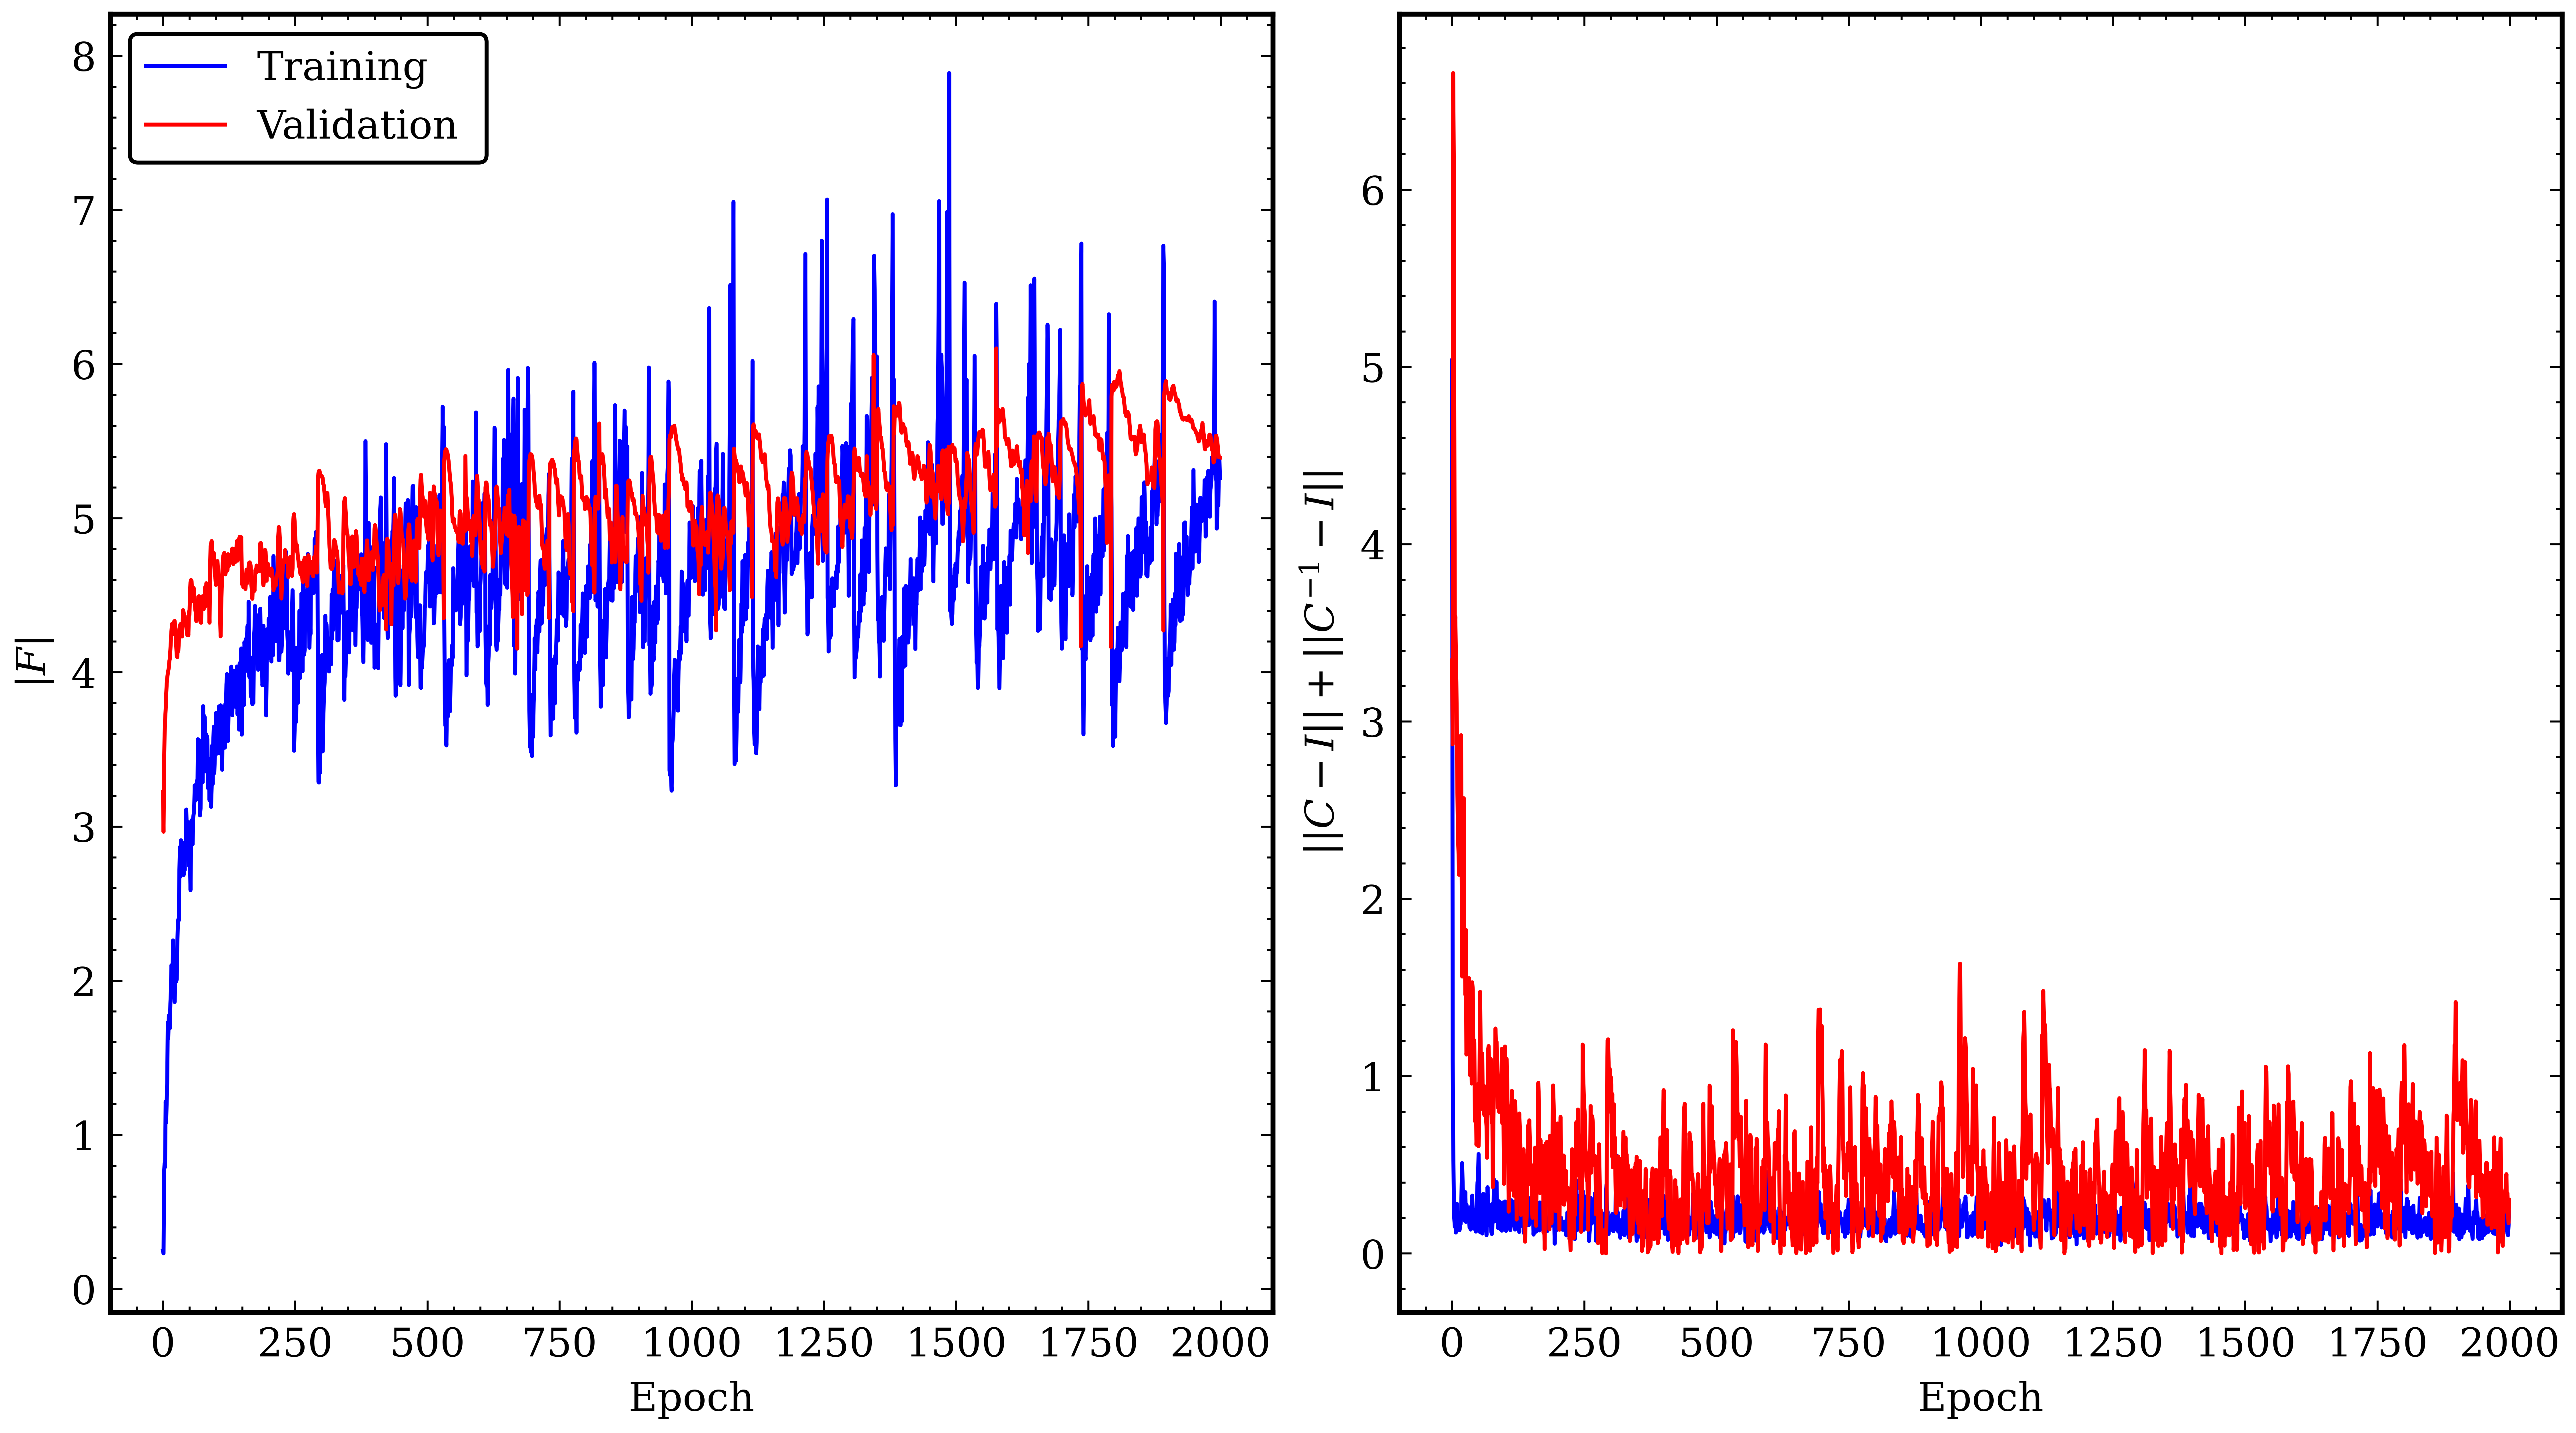
\includegraphics[width=0.95\linewidth]{img/ML/WDM_training_plot.png}
    \caption{$|F|$ and $||C-I ||+||C+I||$ as a function of the epoch for the training and validation sets during the training of the IMNN on the \texttt{SHERWOOD} dataset Lyman-$\alpha$ skewers.}
    \label{fig:IMNN  wdm training}
\end{figure}
In Figure \ref{fig:IMNN wdm training} we show the training progress of the IMNN as a function of the epoch. The information extracted on the validation split quickly saturates at $\sim 250$ epochs. It is clear that the network is able to learn a map from Lyman-$\alpha$ skewers in Fourier space into a one-dimensional parameter space. Since the \texttt{SHERWOOD} suite has a fix number of simulations, interpreting the network output summaries is a challenging task.


\begin{figure}
    \centering
    \begin{subfigure}[b]{0.53\textwidth}
        \centering
            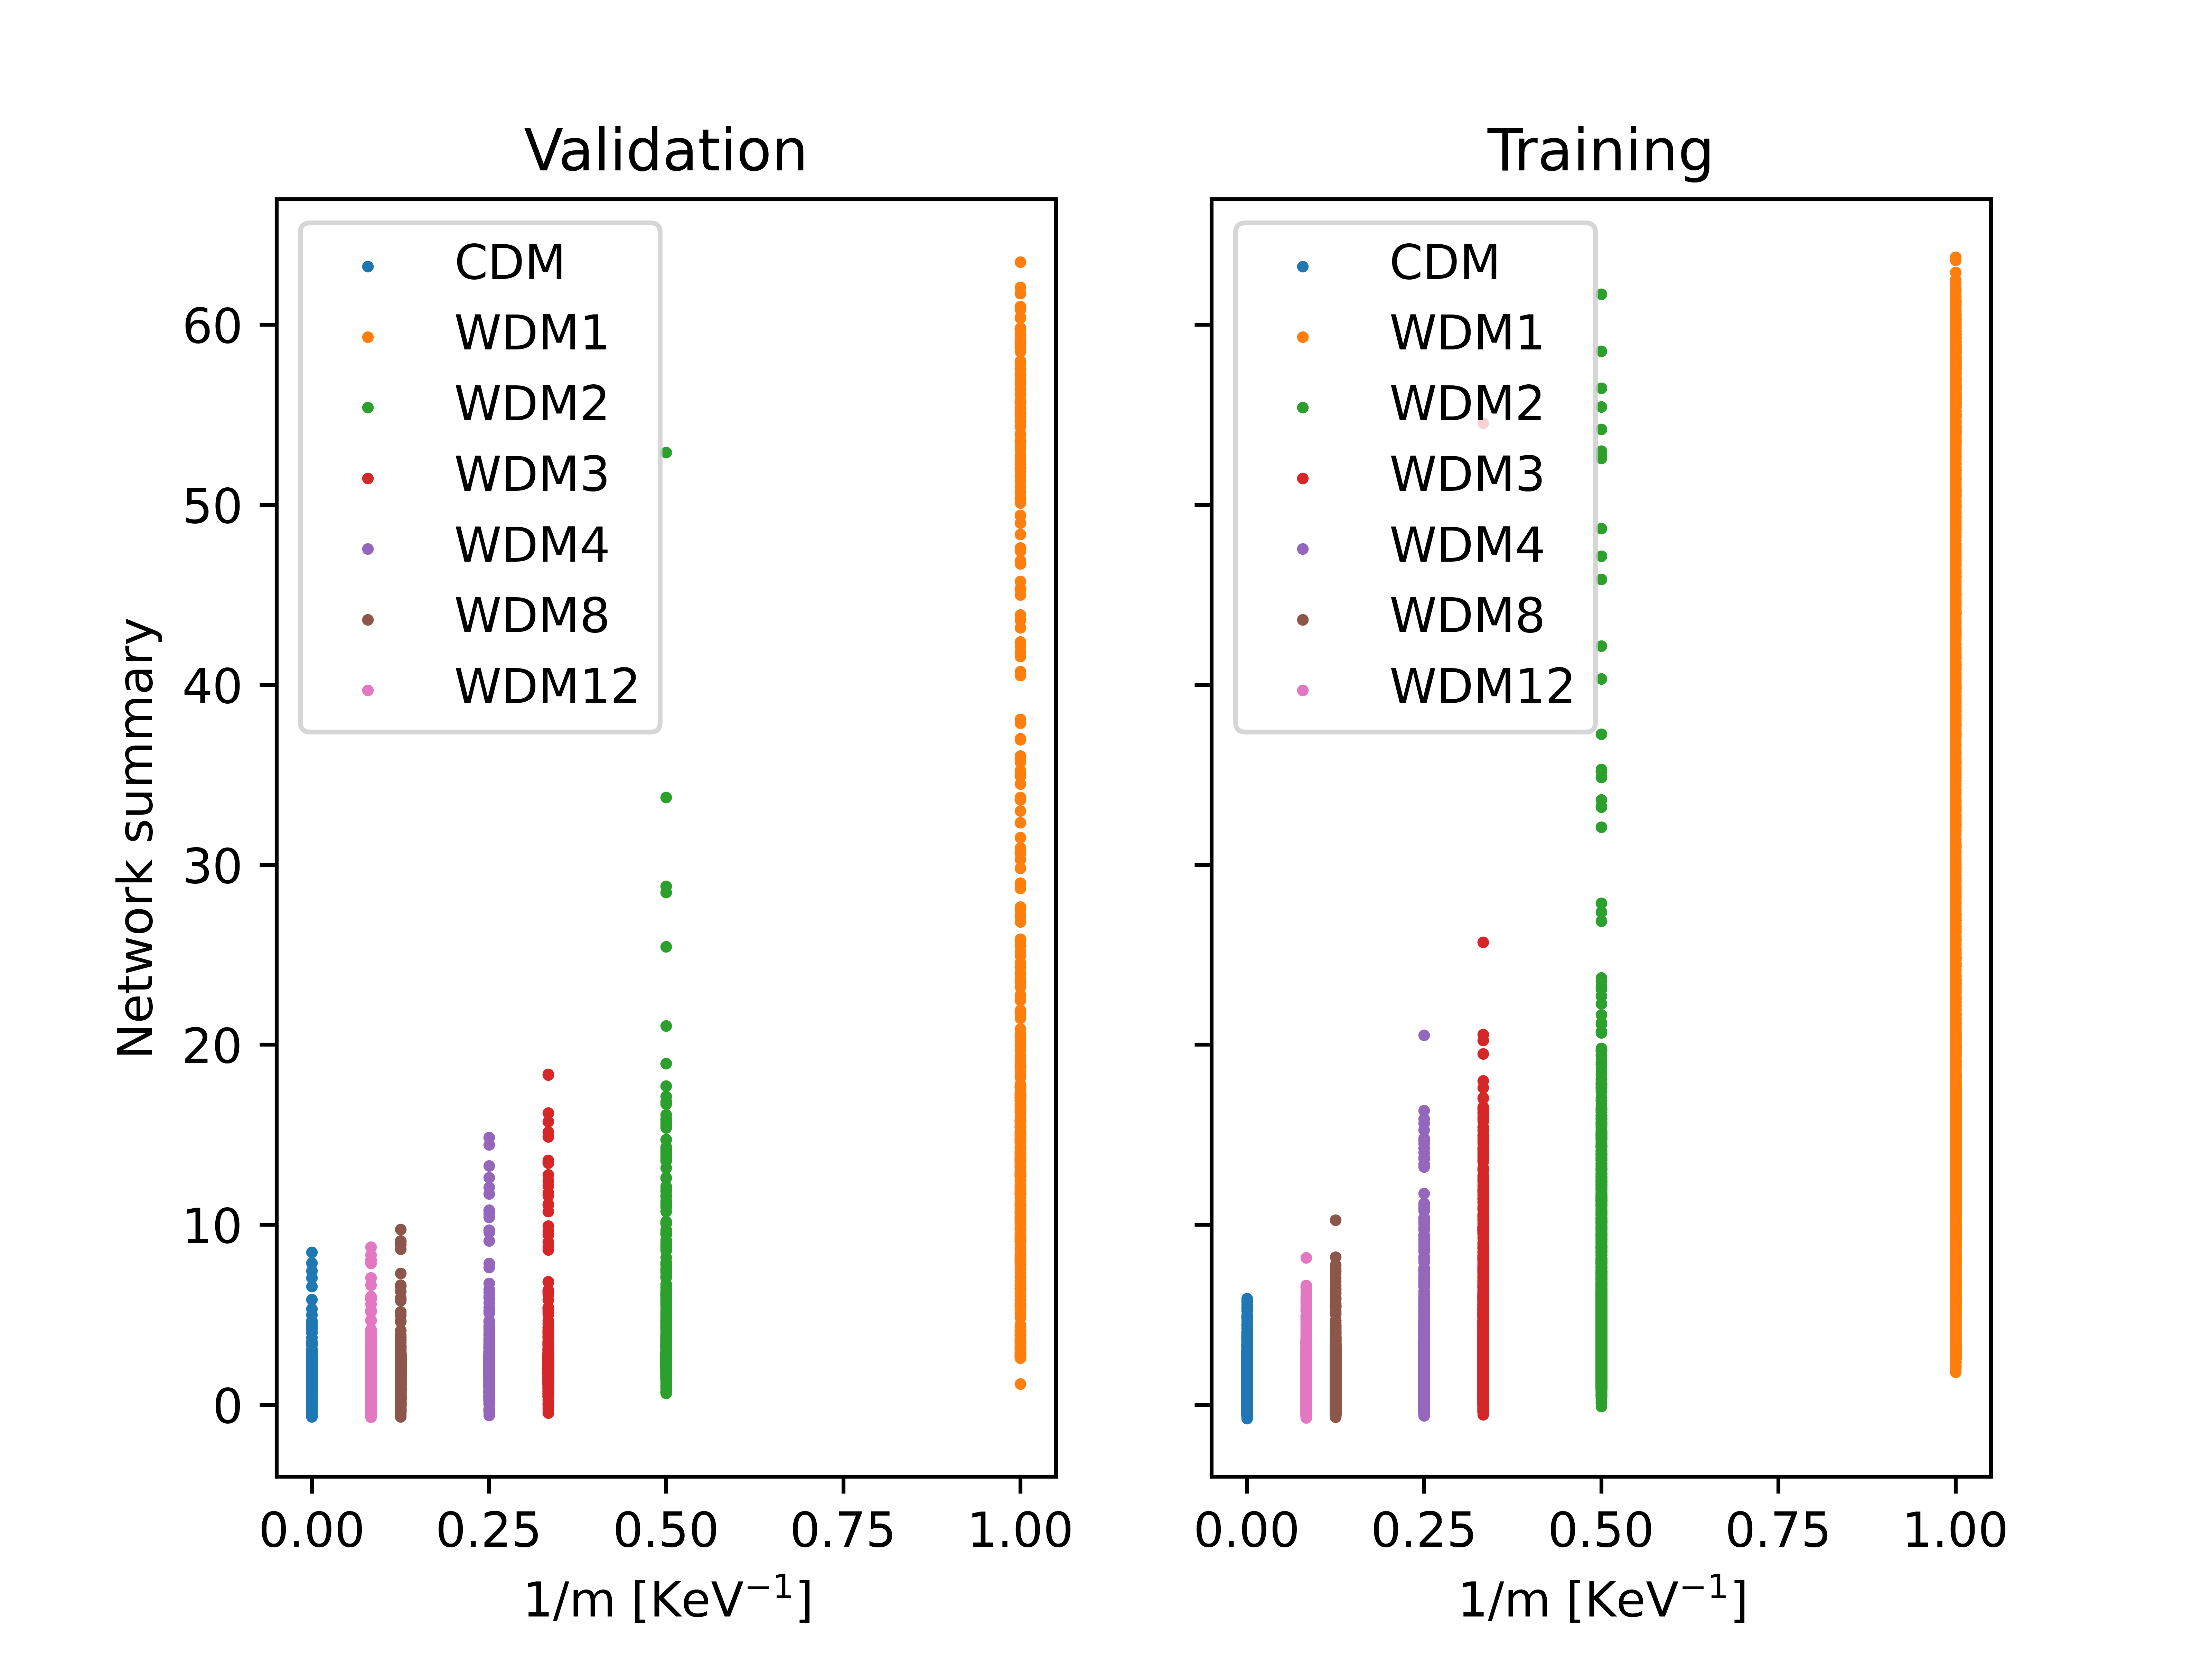
\includegraphics[width=1\textwidth]{img/ML/IMNN_output.png}
            \caption{IMNN outputs for the \texttt{SHERWOOD} Lyman-$\alpha$ skewers.}
    \end{subfigure}
    \hfill
    \begin{subfigure}[b]{0.45\textwidth}
        \centering
        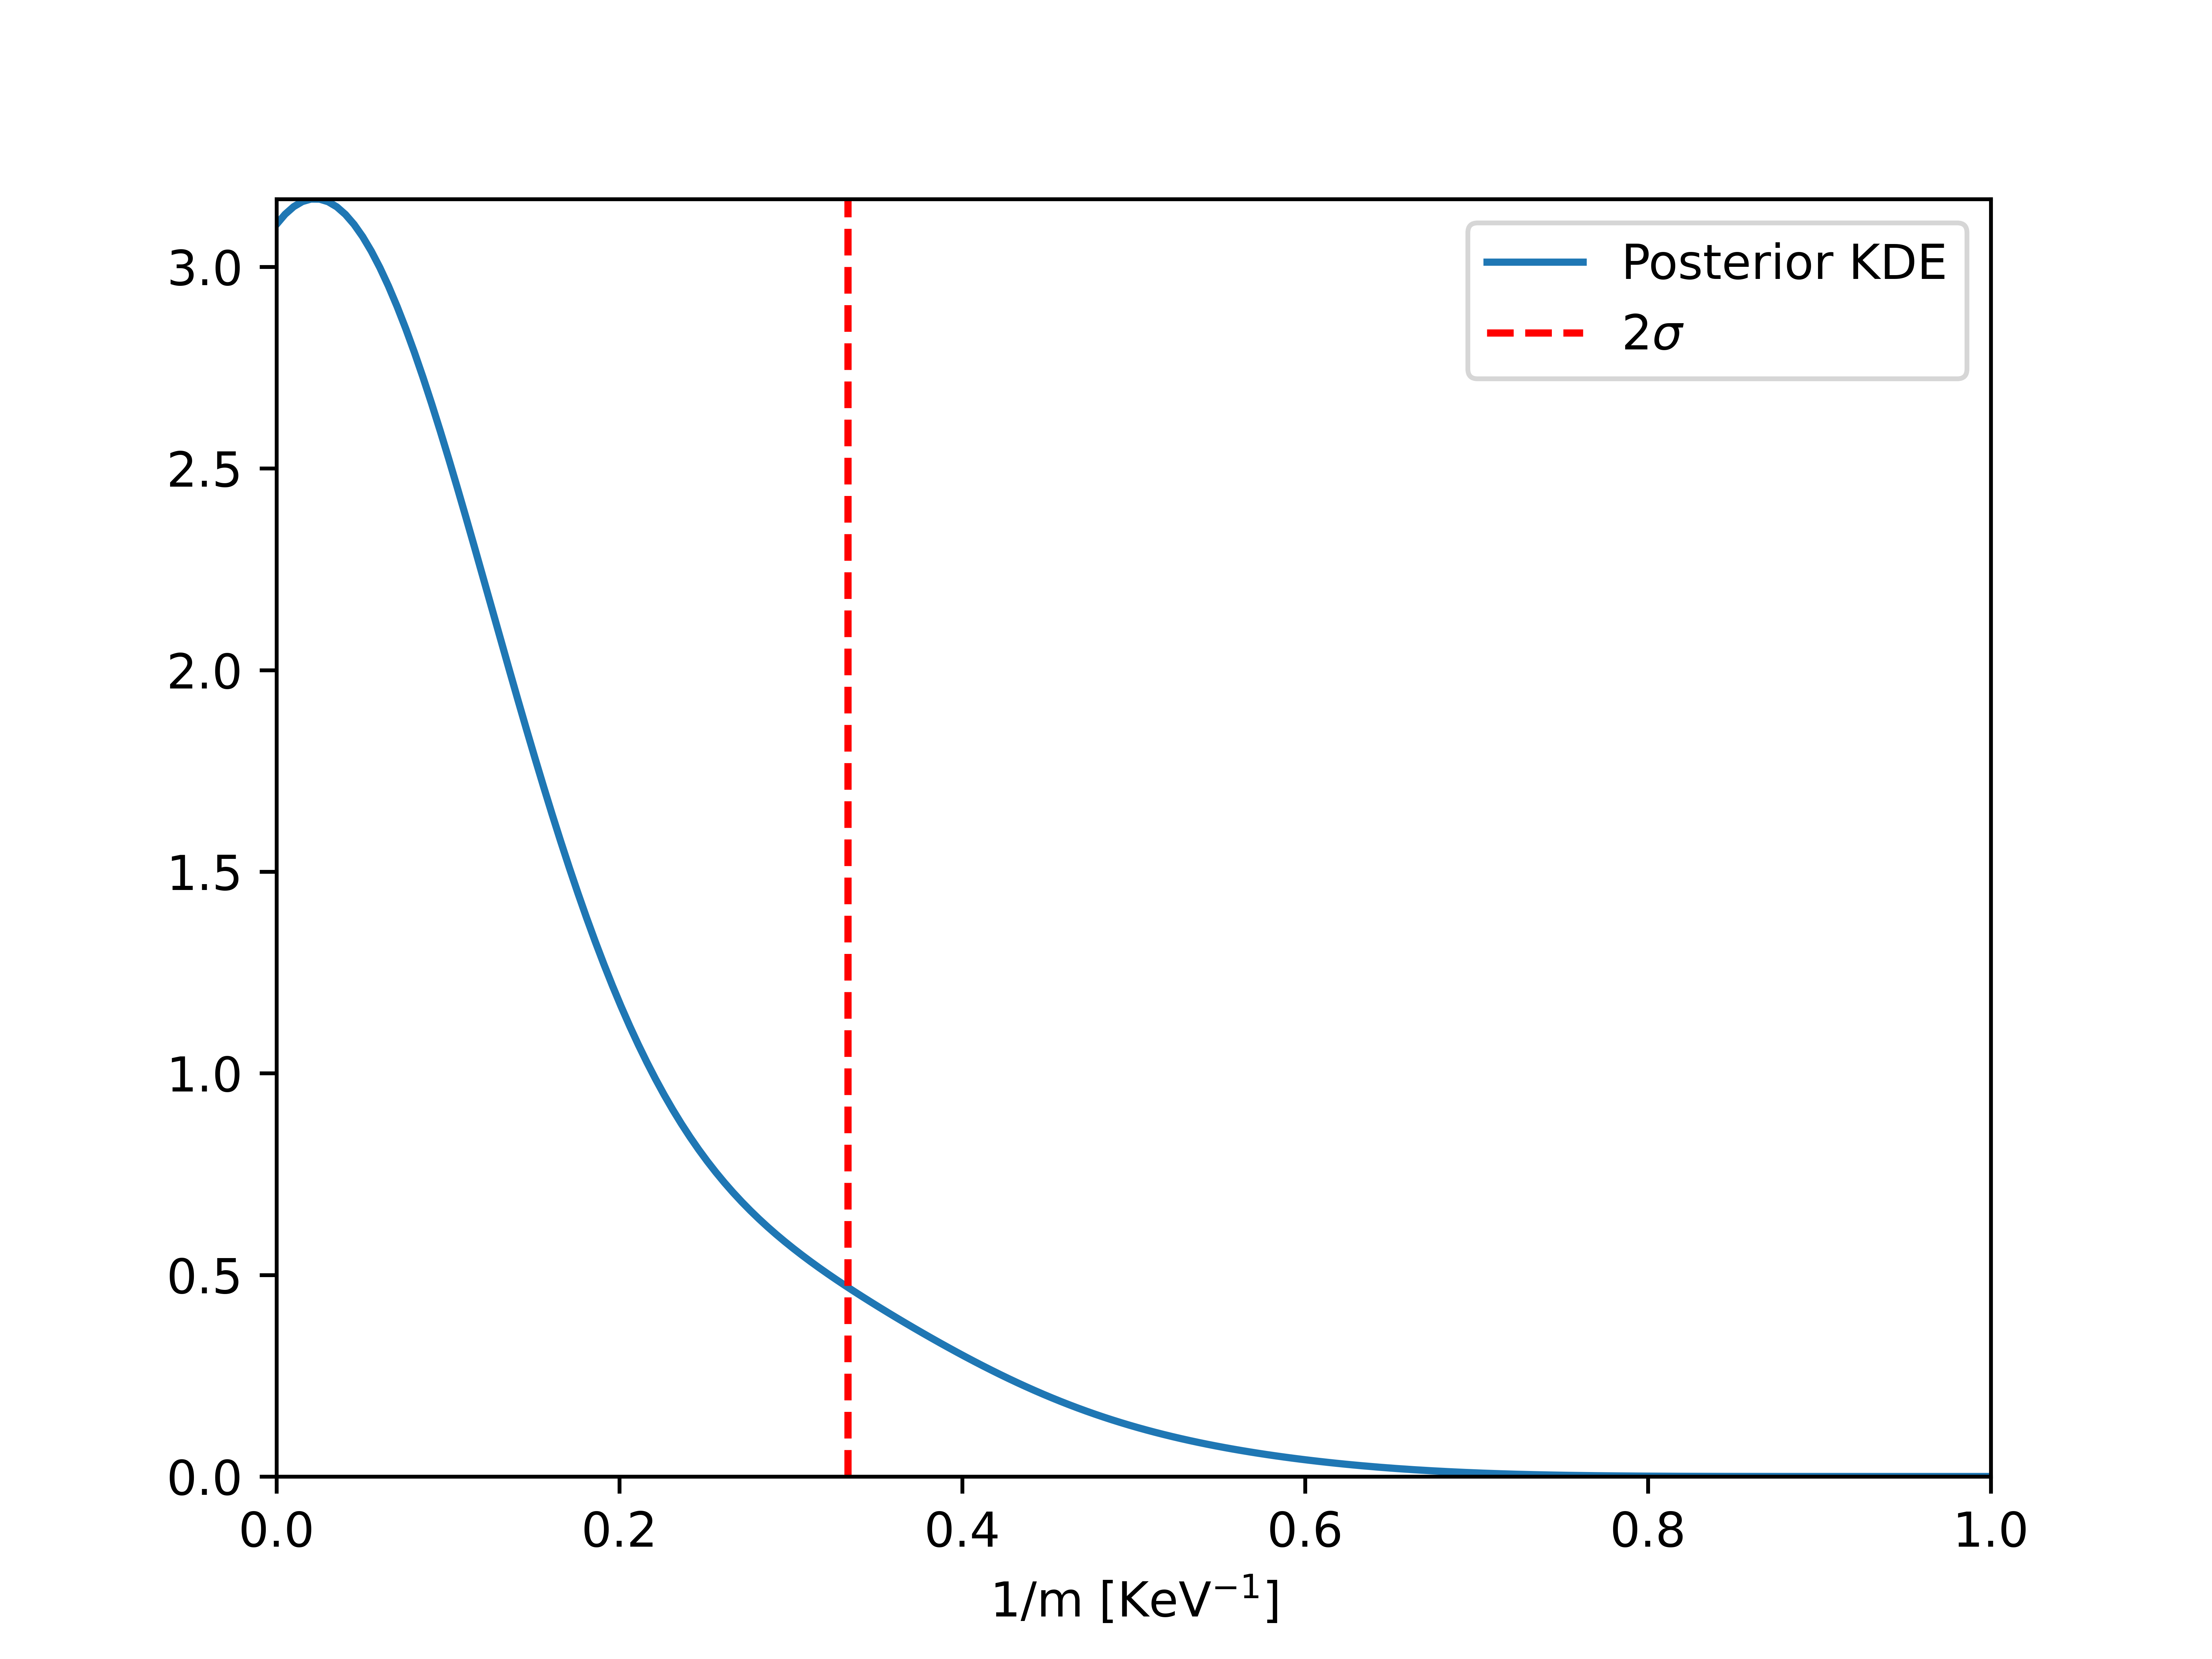
\includegraphics[width=1\textwidth]{img/ML/IMNN_ABC_wdm.png}
        \caption{ABC WDM mass posterior for a test of 50 observed CDM skewers. The $2\sigma$ WDM constraint is $\sim 3 $ Kev.}     
    \end{subfigure}
        \caption{}
        \label{fig:IMNN WDM posterior}
\end{figure}

In Figure \ref{fig:IMNN WDM posterior}a) we show the summaries of the trained IMNN for all the aviable \texttt{SHERWOOD} Lyman-$\alpha$ skewers is Fourier space. Observe how the summaries show a large scatter for every model, corresponding to the large simulation variability within each skewer. However, the mean summaries show a clear bijective trend, manifesting that the IMNN has learnt an informative summary. Note that this can be interpreted as the necessity of a large number of observed samples when constraining WDM models.
We use the IMNN summaries to perform an inference test and obtain a Bayesian posterior as follows. First, we select 50 CDM skewers from the validation dataset and obtain their corresponding summaries by passing them through the IMNN. We now use all validation skewers from the \texttt{SHERWOOD} suite and obtain their summaries. We use the ABC rejection algorithm \ref{alg:ABC} to generate to posterior distribution in Figure \ref{fig:IMNN WDM posterior}b). The $2\sigma$ limit for the WDM mass is $\sim 3$ KeV. Recall that this is a comparable constraint to the one obtained in section \ref{sec:inference squad}. We interpret this not only as a robustness sign of our original pipeline involving a $\chi^2$ fit the $\Delta_\tau$ PDFs, but most notably as a sign that it optimally extracts the majority of the information of the Lyman-$\alpha$ skewers with respect to the WDM mass parameter.



























\chapter{Conclusions}
In this work, we have explored the potential of novel machine learning techniques to constrain warm dark matter in the cosmological context. We began in Section \ref{chapter:intro} with the basics of the current cosmological paradigm. We highlighted the importance of the intergalactic medium in the formation and evolution of structures. Then, we elaborated on how the Lyman-$\alpha$ forest observed on the spectra of quasars can serve as an efficient probe of the state of the IGM, allowing for the extraction of valuable information. We noted the relevance of dark matter in the $\Lambda$CDM model and discussed the key concepts related to it, such as the free-streaming length. We then understood the motivation behind considering alternative models to CDM, such as warm dark matter. Since WDM affects the matter distribution in the IGM, the Lyman-$\alpha$ forest can provide information on its nature. To understand the impact of WDM on the Lyman-$\alpha$ forest, we turned our attention in Section \ref{chap:sherwood} to cosmological simulations. We introduced the key points on how such hydrodynamical simulations are performed and introduced the \texttt{SHERWOOD} simulation suite, which is at the core of this work. Afterwards, we used the \texttt{SHERWOOD} raw data to compute simulated Lyman-$\alpha$ skewers and explored the impact of peculiar velocities and warm dark matter on its structure. For the latter, we introduced two statistics, the power spectrum and the probability distribution function, to understand the flux and density field from a statistical point of view.

Armed with these preliminaries, we were set to start the task of detecting the signatures of WDM in the IGM density field in Section \ref{chap: deep learning}. This involves transforming the Lyman-$\alpha$ information into density information. For this highly non-trivial task, we resorted to neural networks. We motivated their growing use in astronomy and introduced their basic working principles. Then, we focused on how to build a robust Bayesian neural network to recover the optical depth-weighted density from the Lyman-$\alpha$ forest flux. Bayesian networks naturally allow for a quantification of the prediction uncertainty, which is especially relevant when the real data is contaminated by observational effects, such as noise. We discussed the training procedure, based on the \texttt{SHERWOOD} suite, and the hyper-parameter optimisation of the neural network. We then evaluated the accuracy of the trained neural network on the validation data, which is as high $79 \%$ ($1\sigma$), and explored the accuracy of the recovered statistics on the density field and their respective uncertainties. Lastly, we discussed some aspects of the model's interpretability, illustrated by saliency maps and pruning. All in all, in Section \ref{chap: deep learning} we find that it is viable to recover the $\Delta_\tau$ density field from Lyman-$\alpha$ skewers for different WDM models and IGM temperatures, showing that the thermal history and WDM models are not completely degenerate.

In Section \ref{sec: inference pipeline} we leverage our machine learning-recovered density fields to constrain WDM. We build an efficient statistical inference pipeline that fits the recovered $\Delta_\tau$ PDF to the PDF for each WDM model in the \texttt{SHERWOOD} suite and generates constraints on the allowed WDM particle mass. We extensively test the robustness of this pipeline using a set of CDM cosmological simulations obtained from \texttt{Nyx}, an alternative hydrodynamical code based on the Lagrangian framework. For a set of 450 \texttt{SHERWOOD} CDM simulated skewers with $SNR=30$ and a resolution of $6$ km/s per pixel, we find a lower bound on the WDM particle mass of $\sim 10$ KeV at $2\sigma$ confidence. Once successfully tested on simulated data, we apply our inference pipeline to real observational from the UltraViolet-Visual Echelle Spectrograph at the Very Large Telescope and the Gemini High-resolution Optical SpecTrograph at the Gemini South Telescope. The two independent datasets consist of 6 quasar SQUAD DR1 Lyman-$\alpha$ forests at $z=4.4$, and a single target quasar with a forest spanning the redshift range $\sim 4.1-4.9$, respectively. We obtain $2\sigma$ constraints of 3.8 and 4.4 KeV for both of those datasets. Our findings are comparable to state-of-the-art techniques, but require significantly less observed data, highlighting the efficiency of machine learning techniques in extracting information from complex data. We conclude our work by testing a statistic-independent alternative approach using Information Maximising Neural Networks to test whether our constraints can be tightened, but find no significant improvement.

Our work aligns with the ground-breaking introduction of machine learning methods in astronomy and astrophysics in recent years and highlights how such approaches can be used to efficiently extract information from the Lyman-$\alpha$ forest. Future efforts based on this approach can be targeted at jointly constraining multiple physical parameters of interest besides WDM, such as the thermal parameters of the IGM, using a finner grid of simulations. Significant improvement can also be made in designing a fully Bayesian inference method.


\printbibliography

\end{document}
